%% LyX 2.3.6.2 created this file.  For more info, see http://www.lyx.org/.
%% Do not edit unless you really know what you are doing.
\documentclass[english]{scrreprt}
\usepackage[T1]{fontenc}
\usepackage[utf8]{inputenc}
\setcounter{secnumdepth}{3}
\setcounter{tocdepth}{3}
\usepackage{color}
\definecolor{note_fontcolor}{rgb}{0.800781, 0.800781, 0.800781}
\usepackage{babel}
\usepackage{varioref}
\usepackage{float}
\usepackage{calc}
\usepackage{textcomp}
\usepackage{url}
\usepackage{amsmath}
\usepackage{amssymb}
\usepackage{graphicx}
\usepackage{esint}
\usepackage{nameref}

\makeatletter

%%%%%%%%%%%%%%%%%%%%%%%%%%%%%% LyX specific LaTeX commands.
%% Because html converters don't know tabularnewline
\providecommand{\tabularnewline}{\\}
%% The greyedout annotation environment
\newenvironment{lyxgreyedout}
  {\textcolor{note_fontcolor}\bgroup\ignorespaces}
  {\ignorespacesafterend\egroup}

%%%%%%%%%%%%%%%%%%%%%%%%%%%%%% User specified LaTeX commands.
%\usepackage{epstopdf} % to include .eps graphics files with pdfLaTeX
\usepackage{flafter}   % Don't place floats before their definition
%\usepackage{topcapt}  % Define \topcation for placing captions above tables (not in gwTeX)

\usepackage{xurl}      % better URL setting, uses old url package

\usepackage{xcolor}
\definecolor{darkblue}{rgb}{0,0,0.4}
\usepackage[]{hyperref} % Generates all cross references
\hypersetup{            % Setting options for hyperref package
	breaklinks=true,    % break line with long hyperlinks
	colorlinks=true,    % coloured links
	linkcolor=blue,
	filecolor=magenta,
	urlcolor=darkblue,
	citecolor=blue,
	backref=page
} 

\usepackage{memhfixc}  % remove conflict between the memoir class & hyperref
\usepackage{pdfsync}   % enable tex source and pdf output syncronicity

\usepackage{alltt}

\@ifundefined{showcaptionsetup}{}{%
 \PassOptionsToPackage{caption=false}{subfig}}
\usepackage{subfig}
\makeatother

\usepackage{listings}
\lstset{language=Python,
inputencoding=utf8,
extendedchars=false,
frameround=fttt,
numbers=none,
numberstyle={\tiny},
stepnumber=2,
numbersep=9pt,
showspaces=false,
showstringspaces=false,
showtabs=false,
tab={\rightarrowfill},
basicstyle={\small},
keywordstyle={\color{blue}},
commentstyle={\color{green}},
stringstyle={\ttfamily \color{magenta}},
identifierstyle={\color{black}}}
\usepackage[style=authoryear,hyperref=true, backref=true, backrefstyle=three,backreffloats=true,indexing=bib,date=year]{biblatex}
\renewcommand{\lstlistingname}{\inputencoding{latin9}Listing}

\addbibresource{/Users/Theo/Jabref/TransientGroundwater.bib}
\begin{document}
\title{UNESCO-IHE\\
Transient Groundwater Flow, Analytical Solutions}
\author{Prof. dr.ir. T. N. Olsthoorn, PhD, MSc}
\date{\today}

\maketitle
\tableofcontents{}

\chapter*{Nomenclature}

\section*{General}
\begin{description}
\item [{$x,y,z\,\mathrm{\left[L\right]}$}] Coordinates. $z$ is upward
positive relative to top of model, sea level, ground surface, top
of aquifer or any other suitable fixed datum elevation.
\item [{$r\,\mathrm{\left[L\right]}$}] Distance from the well or center
of model in the case of axial symmetric flow. Also used for the radius
of a capillary.
\item [{$R\,\mathrm{\left[L\right]}$}] Radius of influence, outer radius
of circular aquifer or island.
\item [{$t,\,\Delta t\,\mathrm{\left[T\right]}$}] Time.
\item [{$A\,\mathrm{\left[L^{2}\right]}$}] Surface area.
\item [{$V\,\mathrm{\left[L^{3}\right]}$}] Volume.
\end{description}

\section*{Hydraulic and mechanical properties}
\begin{description}
\item [{$\mu\,\mathrm{\left[FT/L^{2}\right]}$}] Water viscosity, e.g.
$\mathrm{\left[Ns/m^{2}\right]}=\mathrm{\left[Pa\,s\right]}$
\item [{$\kappa\,\mathrm{\left[L^{2}\right]},\,k\,\mathrm{\left[L/T\right]}$}] Permeability
(independent of fluid) and hydraulic conductivity. $k=\rho_{w}g\frac{\kappa}{\mu}$.
Note that $\kappa$ and $k$ are vectors, i.e. they are direction
dependent.
\item [{$c\,\mathrm{\left[T\right]}$}] Vertical hydraulic resistance of
aquitards or a low-conductive layer, $c=d/k_{v}$ with $d\,\mathrm{\left[L\right]}$
the thickness of this layer and $k_{v}\,\mathrm{\left[L/T\right]}$
its vertical hydraulic conductivity.
\item [{$S\,\mathrm{[-]}$}] Elastic storage coefficient $\mathrm{\left[L^{3}/L^{2}/L\right]}$
\item [{$S_{s}\mathrm{\left[L^{-1}\right]}$}] Specific elastic storage
coefficient $\mathrm{\left[L^{3}/L^{2}/L\right]}$
\item [{$S_{y}\mathrm{\left[L^{-1}\right]}$}] Specific yield $\mathrm{\left[L^{3}/L^{2}/L\right]}$.
Specific yield is storage from draining pores.
\item [{$\alpha,\,\beta\,\mathrm{\left[L^{2}/F\right]}$}] compressibility
of water and bulk porous matrix respectively. $\beta=1/E$ where $E$
is the compression modulus.
\item [{$E_{w},\,E_{m}\,\mathrm{\left[F/L^{2}\right]}$}] Compression modulus
of water and porous medium respectively. $E=1/\beta$, where $\beta$
is the compressibility.
\item [{$\rho_{w},\,\rho_{s},\,\rho_{b},\,\rho\,\mathrm{\left[M/L^{3}\right]}$}] Density
of water, solids, bulk porous medium respectively.
\end{description}

\section*{Heat properties and flow}
\begin{description}
\item [{$c,\,c_{w},\,c_{s}\,\mathrm{\left[E/M/K\right]}$}] Bulk heat capacity,
heat capacity of water and solids. $c=\epsilon c_{w}+\left(1-\epsilon\right)c_{s}$
\item [{$\lambda,\,\lambda_{w},\,\lambda_{s}\,\mathrm{\left[E/T/L/K\right]}$}] Bulk,
water and solids heat conductance, $\lambda=\epsilon\lambda_{w}+\left(1-\epsilon\right)\lambda_{s}$
\item [{$\epsilon\,\mathrm{\left[-\right]}$}] Porosity of the porous medium
\item [{$\mathbb{D}\,\mathrm{\left[L^{2}/T\right]}$}] For heat flow $\mathbb{D}=\frac{\lambda}{\rho c}$,
i.e. heat conductivity over bulk volumetric heat capacity of water
plus medium, $\lambda=\epsilon\lambda_{w}+\left(1-\epsilon\right)\lambda_{s}$
and $\rho c=\epsilon\rho_{w}c_{w}+\left(1-\epsilon\right)\rho_{s}c_{s}$.
For diffusivity in the context of groundwater flow see under\textbf{
Aquifer system}.
\item [{$\mathbb{R}\,\mathrm{\left[-\right]}$}] Retardation, i.e. the
factor by which transport of mass or heat is delayed relative to that
of the pore water. It is the amount of mass or heat in the water over
the total amount of mass or heat in the water plus sorbed to/in the
grains. Hence for heat $\mathbb{R}=\rho_{w}c_{w}\epsilon/\left(\rho_{w}c_{w}\epsilon+\rho_{s}c_{s}\left(1-\epsilon\right)\right)$
with indices $w$ and $s$ referring to water and grains respectively.
\end{description}

\section*{Aquifer system}
\begin{description}
\item [{$q,\,q_{x},q_{y},\,q_{z}\,\mathrm{\left[L/T\right]}$}] Specific
discharge, which generally is direction-specific (a vector)
\item [{$Q\,\mathrm{\left[L^{3}/T\right],\,\left[L^{2}/T\right]}$}] Discharge.
It can mean the total discharge over the thickness of the aquifer
in a cross section $\mathrm{L^{2}/T}$ or the extraction or injection
of a well, in which case its dimension is $\mathrm{L^{3}/T}$.
\item [{$N,\,\overline{N}\,\mathrm{\left[L/T\right]}$}] Net recharge and
the time or space average net recharge respectively
\item [{$h\,\mathrm{\left[L\right]}$}] Phreatic head, in the case of a
water table aquifer, the head relative to the bottom of this aquifer,
i.e. the wetted aquifer thickness
\item [{$\phi\,\mathrm{\left[L\right]}$}] Head in semi-confined and confined
aquifers, relative to some predefined datum, i.e. sea level.
\item [{$s\,\mathrm{\left[L\right]}$}] Drawdown, or head relative to initial
situation (lower case $s$)
\item [{$p,\,\sigma_{w},\sigma_{s},\sigma_{e}\,\mathrm{\left[F/L^{2}\right]}$}] Pressure,
water pressure, total or soil pressure and effective pressure. $\sigma_{t}$
also used for total pressure.
\item [{$H\,\mathrm{\left[L\right]}$}] Thickness of aquifer. Often used
only for water table aquifer, sometimes for any aquifer.
\item [{$D\,\mathrm{\left[L\right]}$}] Total thickness of aquifer
\item [{$kD\,\mathrm{\left[L^{2}/T\right]}$}] Transmissivity of an aquifer.
$kH$ may be used in an water-table aquifer.
\item [{$T\,\mathrm{\left[T\right]}$}] Characteristic time of a dynamic
groundwater system.
\item [{$\mathbb{D}\,\mathrm{\left[L^{2}/T\right]}$}] Diffusivity. For
flow $\mathbb{D}=\frac{kD}{S}$ for thermal flow $\mathbb{D}=\frac{\lambda}{\rho c}$,
see under Heat
\item [{$\lambda\,\mathrm{\left[L\right]}$}] Characteristic length or
spreading length of a semi-confined aquifer system, i.e. $\lambda=\sqrt{kDc}$
with $kD\,\mathrm{\left[L^{2}/T\right]}$ the aquifer's transmissivity
and $c\,\mathrm{\left[T\right]}$ the aquitard's vertical resistance.
\item [{$R,\,R_{0}\,\mathrm{\left[L\right]}$}] Fixed radial distance to
the center of axial symmetric flow system at which the head is fixed
or zero.
\item [{$LE$}] {[}-{]} Loading efficiency, $LE=\frac{\beta_{m}}{\epsilon\beta_{w}+\beta_{m}}$.
Note that $LE+BE=1$
\item [{$BE$}] {[}-{]} Barometric efficiency. $BE=\frac{\epsilon\beta_{w}}{\epsilon\beta_{w}+\beta_{m}}$.
Note that $LE+BE=1$
\end{description}

\section*{Groundwater waves}
\begin{description}
\item [{$A\,\mathrm{\left[L\right]},\,B\,\mathrm{[L]}$}] Wave amplitude.
\item [{$L\,\mathrm{\left[L\right]}$}] Width of the groundwater system.
\item [{$a$}] Damping factor of groundwater head wave moving through the
aquifer, caused by a kind of tide. $a=\sqrt{\frac{\omega}{2\mathbb{D}}}$
\item [{$\omega\,\mathrm{\left[T^{-1}\right]}$}] or rather radians per
time. The angle velocity of the wave. Full wave time $T=2\pi/\omega$
\item [{$T\,\mathrm{\left[T\right]}$}] Cycle time, time of a full wave.
$T=2\pi/\omega$
\end{description}

\section*{Physics, math and mechanics}
\begin{description}
\item [{$g\,\mathrm{\left[F/M\right]\mbox{, }\left[L/T^{2}\right]}$}] Gravity,
acceleration in the Earth's gravity field or the force with which
the earth's gravity field pulls at a unit mass at ground surface in
the direction of the earth's center.
\item [{$\gamma\,\mathrm{\left[F/L\right]}$}] Surface tension, cohesion
in capillary systems.
\item [{$\mbox{IR}\left(\tau\right)\mbox{, }BR\left(\tau,\Delta\tau\right)\mbox{, }SR\left(\tau\right)$}] Respectively:
Impulse response, Block response, Step response of a system. $\Delta\tau$
step size, $\tau$ lapsed time since event started. See chapter on
convolution.
\item [{$\mbox{erfc}\left(u\right)$}] Complementary Error function, i.e
$\mbox{erfc}\left(u\right)=\frac{2}{\sqrt{\pi}}\intop_{u}^{\infty}e^{-\zeta^{2}}d\zeta$,
and, therefore, $\frac{d\mbox{erfc}\left(u\right)}{du}=-\frac{2}{\sqrt{\pi}}e^{-u^{2}}$
\item [{$\mbox{W}\left(u\right)$}] Theis' well function, for transient
flow to a well in a confined aquifer, i.e. $\mbox{W}\left(u\right)=\mbox{iexp}\left(u\right)=\intop_{u}^{\infty}\frac{e^{-\zeta}}{\zeta}d\zeta$,
iexp is the exponential integral.
\item [{$\mathrm{W}\left(u,\frac{r}{\lambda}\right)$}] Hantush's well
function for semi-confined transient flow to a well, $\mbox{W}\left(u,\frac{r}{\lambda}\right)=\intop_{u}^{\infty}\frac{1}{\zeta}\exp\left(-\zeta-\frac{1}{4\zeta}\left(\frac{r}{\lambda}\right)^{2}\right)d\zeta$
\item [{$u\,\mathrm{[-]}$}] In 1D (cross sections as argument of the $\mbox{erfc}$-function),
$u=\sqrt{\frac{x^{2}S}{4kDt}}$. In axial symmetric situations, as
argument of the Theis and Hantush solutions, $u=\frac{r^{2}S}{4kDt}$
\item [{$\mbox{I}_{o}\left(z\right)\mbox{, }\mathrm{I}\left(z\right)\mbox{, }\mathrm{K}_{o}\left(z\right)\mbox{, }\mathrm{K}_{1}\left(z\right)$}] dimensionless
modified Bessel function using in axial-symmetric semi-confined steady-state
solutions. They depend on the scaled distance $z=r/\lambda$, with
$\lambda=\sqrt{kDc}$
\end{description}

\chapter{Introduction}

This syllabus has been prepared as part of the IHE master's program
in Hydrology and Water Resources, at IHE Delft, The Netherlands. The
part given by the author, i.e. transient analytical solutions, consists
of a total of 18 lecture hours divided over four and a have days.
The majority of ours will be oral lectures and a minority will be
practical exercises in which the students learn to solve their problems
by implementing the groundwater solutions in Python.

The material for this course will be stored on\textbf{ Github} (\url{https://github.com}).
Search for \emph{Theo Olsthoorn} combined with \emph{github} and or
\emph{TransientGroundwater} to find the site an or pictures of me.
The material includes \emph{Jupyter notebooks} that were used to generate
most of the figures in this syllabus.

\section{Objectives of the course}
\begin{itemize}
\item The students will become familiar with the basic 1D and axially symmetric
transient groundwater solutions that can readily be applied in practical
situations when a computer models is not readily available, where
a fast idea of the effect of groundwater impacts is required, where
a model is to be verified and so on.
\item Students will learn how to deal with and apply superposition, which
is perhaps the most important tool to handle more complex systems
with analytically.
\item Students will obtain insight in the transient behavior of groundwater
systems, and learn to reason based on their characteristics such as
halftime and the relations between parameters and the way parameters
workout in the effect on the system.
\item Students will learn to simplify analytical solutions to extract behavior
characteristics that are easy to understand and apply for under specified
conditions.
\item Closed analytical solutions for transient groundwater flow are only
available for linear systems, i.e. systems with a constant transmissivity
and storativity. Students will learn how to deal in an approximate
way with situations where transmissivity will vary due to extractions
or injections of water.
\item Students will gain insight in the behavior of real-world groundwater
systems and learn how to read their reaction.
\item Students will also learn what physics cause a given behavior of groundwater
systems. Storage characteristics and barometric and tidal reactions
will be dealt with.
\item Students will learn and exercise how to implement transient analytical
solutions in Python and visualize their results.
\item Students will learn how to analyze basic pumping tests to obtain the
parameter values of a groundwater system.
\item Depending on the group, students will learn how to handle complicated
time varying systems by means of convolution.
\item Students will carry out an assignment in which they apply the various
aspects they've learned.
\end{itemize}

\section{Exam}

The exam is closed-book and will last one hour. It consists of solving
several tasks and providing answers to questions concerning the text.
Required formulas will be given.

\section{Assignment}

An assignment will be provided. It can be partially made in class
during the exercises in the afternoons. I must have the results when
I judge your written exams, that is, by the end of the week in which
the written exam takes place, simply because I can't give marks without
the assignments. Any assignments handed in thereafter will not be
graded, which implies that the entire mark will be defined only by
the results of the written exam.

It is clear that I expect everyone to do his/her own assignments.
It is generally easy for me to see who copied his or her work from
someone else.

\section{Gradiing}

Grading will be 70\% for the exam, 30\% for the assignments.

Answers given during the exam must show their motivation, that is,
the rationale: I want to see what (mental) steps you make. So motivate
each step with some clarifying words. Just numbers or incomprehensible
formula derivations do not count!

\section{What to learn / understand}
\begin{enumerate}
\item Sections \ref{chap:Introduction-to-transient} through \ref{sec:Elastic-Storage}.
Check yourself by answering the questions. Skip section \ref{sec:Earth-tides}.
\item Sections \ref{sec:Scope-5-1} through \ref{sec:Sinusoidal-fluctuations},
to the extent that you understand and can answer the questions in
section \ref{subsec:Questions-5-3-5}. 
\item Sections \ref{subsec:Basins-of-half-infinite-lateral-extent} through
\ref{subsec:Questions-5-4-2}. Understand how the erfc function works,
understand that that the differential equation is a water balance,
and understand what the parameters in the solution mean. Answer the
questions in section \ref{subsec:Questions-5-4-2}.
\item Skip section \ref{sec:Higher-level-solutions} and \ref{subsec:Questions-5-4-4};
they may be useful as a future reference.
\item Section \ref{subsec:Superposition-in-time-half-inf-aquifer}. Understand
how superposition in time works, and how to apply it when the analytic
solution is provided.
\item Sections \ref{subsec:Introduction-5-5-1} through \ref{subsec:Questions-5-5-5}.
Understand how superposition in space works. Answer the questions
of section \ref{subsec:Questions-5-5-5}.
\item Section \ref{sec:Symmetrical-drainage-from-charcteristic-time}. Understand
what the formula in section \ref{subsec:Analytical-solution}means
and how we cracked it down to a characteristic time for groundwater
systems and to their halftime in section \ref{subsec:Long-term-drainage-behavior-drainage}.
Check if you can answer the questions in section \ref{subsec:Questions-5-6-3}.
\item Chapter \ref{chap:Transient-flow-to-wells}: transient flow to wells.
\item Section \ref{sec:Introduction-6-1} and \ref{sec:Wells-and-well}:
introduction to wells.
\item Section \ref{sec:General-relation-between-well-solutions}, Theis:
Relation between the transient and steady-state well solutions. The
Theis solution and its approximation.
\item It’s always good if you exercise to derive the basic differential
equations (i.e. the physics) yourself. This is, in fact, a basic engineering
skill as it specifies the physics of the problem. Realize that these
partial differential equations are always water balances for an arbitrary,
infinitesimally small portion of the aquifer.
\item Section \ref{sec:Theis-and-Hantush-wells}: Understand the situation
covered by the Theis and Hantush solutions. Understand the behavior
of these solutions on double log and half log axes. Understand where
the extracted water comes from in both cases. Understand that Theis
is a special case of Hantush. Understand how the simplified Theis
solution is derived and why its useful. Understand the radius of influence.
Understand the discharge at distance in the Theis case and what it
implies. What are type curves?
\item Section \ref{sec:Pumping-test-analyses} Pumping tests: Understand
the concept of a pumping test. The interpretation of a pumping test
in the Theis situation using the simplified logarithmic approximation
of the well function (the trick to always determined the transmissivity
from the drawdown per log-cycle of time. The way to determine the
storage coefficient using the simplified log-approximation of the
Theis function and it is limitation (partial penetration, clogged
pumping well when measuring when measuring level inside the pumping
well).
\item Understand the principle of the classic analysis of pumping tests
in the Theis and Hantush situation using graphs and type curves on
double logarithmic scales (or paper).
\item Section \ref{sec:Partial-penetration-of-well-screens} Partial penetration
of the well screen in the aquifer: Just understand what it is and
what effect it has on the drawdown near the well. You an always use
this section as a reference in the future. Only understand the mechanism,
as you are likely to encounter it in practice.
\item Chapter \ref{chap:Convolution} Convolution: Understand what convolution
is. Convolution is extremely useful as it allows to simulate groundwater
with simple formulas for arbitrarily varying input in an efficient
and very general way. It can be seen as a smart form of superposition.
\item Chapter \ref{chap:Laplace-solutions} Laplace solutions: Skip. May
be used as a reference.
\end{enumerate}

\section{Note with respect to the exercises}

Nowadays, there are two skills that students should acquire to be
able to do sound quantiative analysis like it is the case in this
course: Python and QGIS. My motivation is as follows:

With Python, there is no limit to what you as student of professional
may compute (and visualize) on your laptop,. Neither is there any
practical limit to the amount of data you can handle and process,
or the complexity you can handle. And, perhaps the best of it: it
is free of charge.

With QGIS there is no limit to the spatial data you can handle, analyze
and process. And it is also free of charge.

With these two tools you equip yourself for the future as an engineer
or scientist. Both Python and QGIS are free, which is a unique feature
of our time. Never before was so much computing power available to
everybody. And, nobody can ever take it from you, just because it's
free, always present for you to exploit it on your own laptop. Therefore,
it is only up to you yourself to acquire the skills to use it. To
help you, there is an immense amount of resources and information
on the internet about both these tools, so you should never be without
an answer to your questions. There are also numerous tutorials on
the Internet, both written and on video, and, of course, there exists
a large pile of books. Python and QGIS, which have been widely around
for only about 1.5 decades, have already changed the world for engineers
and scientists and are continuing to do so every day. So if you don't
want to be left behind, pick it up. My advice to you, dear students,
is to start using both Python and QGIS for all your projects from
now on.

The exercises for this course will be done in IPython notebooks (now
called \emph{Jupyter notebooks}), which are a terrific means to communicate
your work with others, including your teachers. These notebooks, which
were originally developed for Python only, have since a few years
been extended to over 47 other computer languages, like\emph{ R} and\emph{
Julia}. That is why the name was changed from IPython notebooks to
\emph{Jupyter} notebooks. These notebooks allow you to combine, text,
formulas and code, neatly formatted, while computations are done and
visualized within the notebook itself. Therefore, if your notebook
is correct, then your work is correct. And because the text, with
formulas, code and graphical results can be nicely formatted within
the notebook, the notebook is also a great means for sharing your
results as a living document or, if you like, as a pdf document, which
you can send to your teacher if he/she does not have or know Python.
\begin{itemize}
\item To convince yourselves read what Nature (world's most famous scientific
journal) said about \emph{Ipython notebooks} in 2014:
\end{itemize}
\url{https://www.nature.com/news/interactive-notebooks-sharing-the-code-1.16261}
\begin{itemize}
\item If you want some examples and tutorials see:
\end{itemize}
\url{https://github.com/Carreau/iPython-wiki/blob/master/A-gallery-of-interesting-IPython-Notebooks.md}

\url{https://github.com/iPython/iPython/wiki/A-gallery-of-interesting-IPython-Notebooks}
\begin{itemize}
\item Just do a few of the examples. You'll see that you can reach out over
the entire internet, and could even embed a live webcam from home
(or from your data loggers, of course) in your own notebook.
\item For exploratory computing, which is what you'll be doing most of the
time, see: Search for Exploratory computing Mark Bakker to find his
\emph{github} site from which you can copy the tutorial examples that
he uses to teach Python to 2nd year students of the TUDelft.
\item A \emph{Jupyter notebook} implies: 1) Rich web client. 2) Text and
Math 3) Code 4) Results 5) Share and reproduce
\end{itemize}
For this see

See \url{https://www.dataone.org/sites/default/files/sites/all/documents/perez2017webinar_sm.pdf}

---

Theo Olsthoorn, Dec. 2017/ Jan 2021/ May 2022

\chapter{\label{chap:Introduction-to-transient}Introduction to transient
phenomena in groundwater}

Transient phenomena can only occur if there is some form of storage
for water under pressure. Without storage, at least theoretically,
all changes of water pressures would spread out with infinite speed
across the entire medium. The studied system would then always be
in steady state. Clearly, this is never the case in physical reality.
Every groundwater system has ways to store and release water under
changes of pressure. The specific change of water volume in the porous
medium per unit change of pressure (or head) determines the transient
behavior of the groundwater system.

Under confined groundwater-flow conditions, part of the storage comes
from compressibility of the porous medium and part from the compressibility
of the water. Under conditions of a free water table, i.e. under unconfined
flow conditions, meaning when a free water table is present, also
called phreatic groundwater, most storage comes from filling and emptying
pores above the water table and only a minor part from elastic storage.
The elastic storage is about two orders of magnitude smaller than
the phreatic storage. Because of this, elastic storage is mostly neglected
for aquifer systems with a free water table.

Groundwater systems can be very slow and very fast. Whether a groundwater
system is slow of fast depends on factors that we will study later
in section \vref{subsec:Long-term-drainage-behavior-drainage}. An
example of a very slow groundwater system, one that takes tens of
thousands of years to reach equilibrium, is presented in figure~\vref{fig:Gradual-decay-of-of-mound-Kalahari-DeVries1984},
which shows the ongoing decay of the groundwater mound in the Kalahari
Desert since the last wet episode, which happened some 12500 years
ago \parencite{Vries1984}. The line along which the cross section
was made is shown in figure \vref{fig:Approximately-500-km-kalahari-cross-section-line}
together with the elevation profile.

\begin{figure}
\begin{centering}
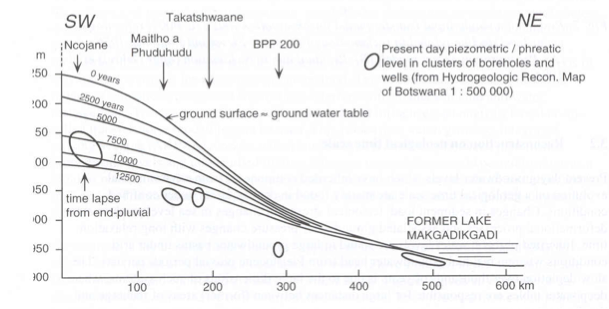
\includegraphics[width=0.8\textwidth]{pictures/KalahariDeVries1984}
\par\end{centering}
\caption{\label{fig:Gradual-decay-of-of-mound-Kalahari-DeVries1984}Gradual
decay of the water table in the Kalahari Desert \parencite{Vries1984}.}
\end{figure}

\begin{figure}
\begin{centering}
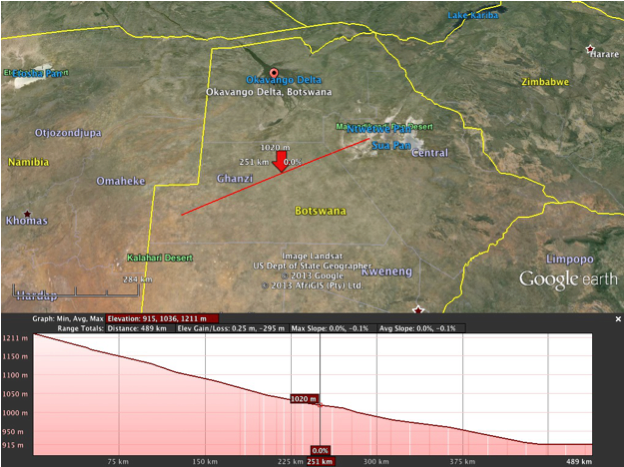
\includegraphics[width=0.8\textwidth]{pictures/line-of-kalahari-cross-section}
\par\end{centering}
\caption{\label{fig:Approximately-500-km-kalahari-cross-section-line}Approximately
500 km long cross section studied by \parencite{Vries1984}, the water
table of which is shown in figure \vref{fig:Gradual-decay-of-of-mound-Kalahari-DeVries1984}}
\end{figure}

Dynamics of groundwater may also be divided into\textbf{ reversible}
and\textbf{ irreversible} behavior. In this syllabus, we will deal
with reversible systems only. Forms of irreversible storage may nevertheless
be important under specific circumstances, or may even be quite common.
Therefore, we will start with an illustration of some forms of irreversible
transient behavior of water-filled porous media.

\chapter{\label{chap:Irreversible-transient-phenomena}Irreversible transient
phenomena}

\section{Consolidation}

One possible form of volume change is due to reordering of ground
particles, which may happen due to an increase of the effective pressure
(= grain pressure), and is characterized by the squeezing out water
which leads to an irreversible decline of pore space. This phenomenon
is called consolidation and leads to land subsidence. The effective
stress, $\sigma_{e}$, is the pressure transmitted between the grains.
Consolidation is especially well known for clay. In clay, under increased
effective stress, micrometer-scale clay plates get reordered and the
pore space thus becomes irreversibly smaller.

As long as grain stresses on vertical planes are horizontal, as is
the case in undisturbed horizontal sediments, the total vertical stress,
$\sigma_{z}$, (in following chapters we will often use the symbol
$p$ instead of $\sigma_{e}$, but they are the same), working on
a horizontal plane in the subsoil always equals the total weight above
this plane. This weight includes possible loads on ground surface.
The total vertical stress $\sigma_{z}$ itself is the sum of the water
pressure, $\sigma_{w}$, and the effective vertical stress $\sigma_{e}$

\[
\sigma_{z}=\sigma_{w}+\sigma_{e}
\]

If we increase the vertical stress, for instance by loading the surface
with a layer of sand, or by filling a surface reservoir, or due to
rainwater infiltrating during the winter season, both stresses will
change

\[
\Delta\sigma_{z}=\Delta\sigma_{w}+\Delta\sigma_{e}
\]

If the water pressure changes, while the total weight remains constant,
as is the case when we lower the head in a confined aquifer (reflect
on why this must be so?), then the water pressure and the effective
stress are directly related

\begin{eqnarray*}
0 & = & \Delta\sigma_{w}+\Delta\sigma_{e}\\
\Delta\sigma_{w} & = & -\Delta\sigma_{e}
\end{eqnarray*}

Therefore, if we lower the head, i.e. the water pressure, the effective
stress increases and the water pressure decreases. This works the
other way around in case the head were increased instead of lowered.

It follows that the lowering of the water pressure puts the grains
of the porous medium under higher stress, which may, therefore, lead
to (irreversible) subsidence in vulnerable soils.

An increased effective stress causes a reduction of the volume of
the porous medium and, therefore, also of its pore space. To compensate
for this reduced space, water will be squeezed out. The speed at which
this happens depends on the conductivity of the compressed layer as
well as its thickness, as with thicker layers it takes more time for
the compressed water to reach the top or bottom of the layer, from
which the water could escape.

Large-scale groundwater extractions have, therefore, led to large
subsidences affecting large areas in, among others, Mexico, USA and
the UK (figure \vref{fig:subsidence-in-the-UK}).

\begin{figure}
\begin{centering}
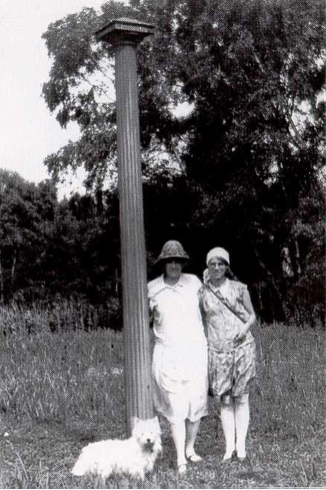
\includegraphics[width=0.5\textwidth]{pictures/subsidenceUK}
\par\end{centering}
\caption{\label{fig:subsidence-in-the-UK}Over $3\mbox{m}$ subsidence in the
UK}
\end{figure}

\begin{figure}
\begin{centering}
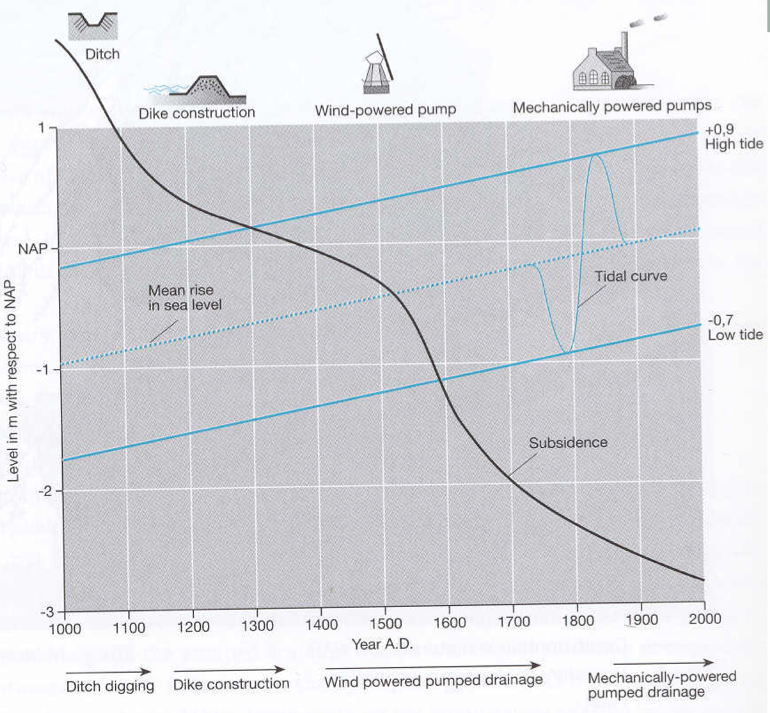
\includegraphics[width=0.6\textwidth]{pictures/ongoingSubsidenceInTheNetherlands}
\par\end{centering}
\caption{\label{fig:Rising-sea-level-and-subsidence-in-the-Netherlands}Rising
sea level since the year 1000 with tide fluctuation curve and subsidence
(descending curve) all relative to mean sea level (about NAP in the
figure). Also shown are water management technologies available over
time \parencite{DufourF2000}}
\end{figure}

Subsidence can be relatively fast (happening within weeks) or slow
(taking place over centuries) on local to regional scales.

Subsidence also occurs as a result of drainage of wetlands and peat
areas. Peat means organic soil, which can decay. This lowering of
the shallow water table also increases the effective stress as we
saw above. This subsidence is especially evident in a low country
like the Netherlands, where drainage of wetlands by ditches has taken
place for about thousand years.

With regard to organic soils, called peat, it is not only the increase
of the effective stress caused by drainage that causes the subsidence.
It is also the entry of oxygen that can enter peaty soils when they
are drained. This oxygen causes oxidation (a kind of natural \emph{burning})
of the peat, giving an extra boost to the subsidence. Subsidence caused
by oxidation may continue until it all peat has disappeared!

The peaty areas in the west and north of the Netherlands have thus
subsided several meters (figure \vref{fig:Rising-sea-level-and-subsidence-in-the-Netherlands}).
This is why about half the Netherlands lies nowadays below sea level.

In case the original soil layers consisted of alternations of peat
and clay, as they often do, the shallow subsoil will consist more
and more of pure clay at the top where all peat was burnt away by
oxidation, with the original mixture still present below the water
table. This clay layer at the top is the collection of all the clay
that was present in the original profile, which may have been several
meters thick.

\section{Liquefaction}

Another irreversible phenomenon involving reordering of grains, is
known as liquefaction, which can happen very fast and spectacularly.
Liquefaction is associated with pressure waves, or shocks. Fine sand
may have been at rest for thousands of years, even with its pore space
being greater than according to the most dense packing of the grains.
In the case of a shock, for instance due to an earthquake, the sudden
change of water pressure may be so great as to cause the effective
stress to be zero for a fraction of a second, during which the grains
lose their mutual friction. The ground then loses its internal friction
and momentarily turns into a quicksand. In fact, it suddenly becomes
a dense liquid in which grains float as freely moving particles. The
matrix will resettle within minutes at a smaller overall volume. During
this resettling, the pore water no longer fits between the grains
in their denser packing. As soon as the surplus water has escaped
the soil resettles and everything sunk into the heavy liquid is stuck
forever (see figure  \ref{fig:Liquefaction-in-Alaska-1964}).

\begin{figure}
\begin{centering}
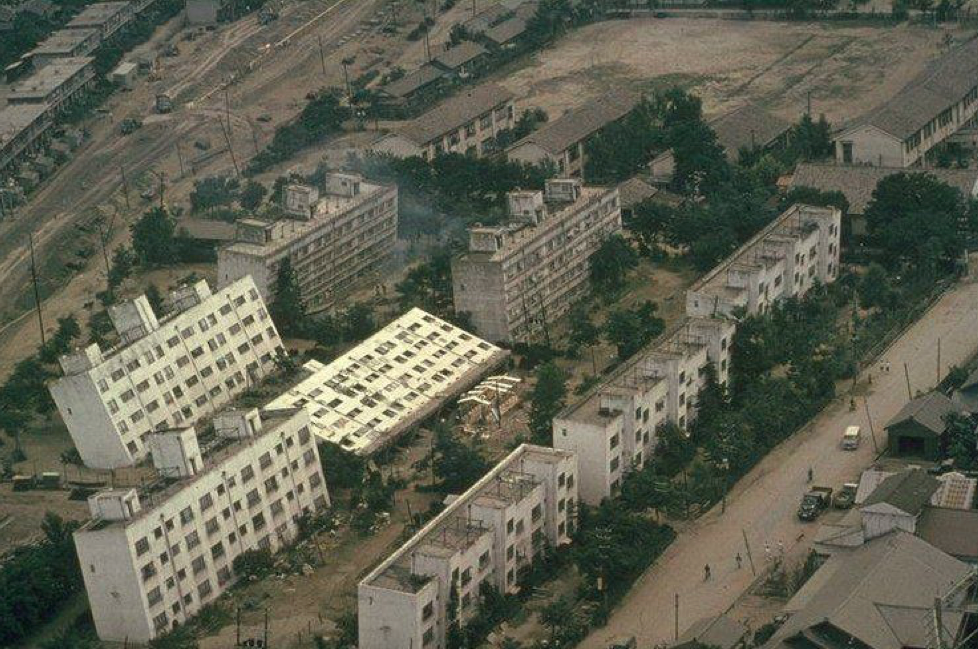
\includegraphics[width=0.8\textwidth]{pictures/liquifactionAlaska1964}
\par\end{centering}
\caption{\label{fig:Liquefaction-in-Alaska-1964}Liquefaction in the USA (see
\protect\url{http://www.ce.washington.edu/~liquefaction})}
\end{figure}


\section{Intrusion of salt water}

In many regions, especially deltaic regions, fresh groundwater floats
on saline water, which is heavier (denser) than fresh water. (The
difference in density between fresh and ocean water is about 2.5\%).
The fresh groundwater in the Netherlands is largely floating on salt
water as is shown in the cross section in figure \ref{fig:Dynamically-floating-fresh-water-in-the-Netherlands-cross-section}.
It will generally take several hundred years to a thousand years for
a freshwater lens to build up from natural precipitation. The equilibrium
may easily be disturbed by extraction of fresh water, but also by
construction of harbors, canals and polders. This will cause upconing
of salt water from below and lateral intrusion of salt water into
aquifers along the coast. Given the time it takes to restore such
systems under natural conditions, mining of these systems may be considered
irreversible under many practical situations as there are no real
means (or sufficient fresh water) to restore the systems within the
time horizon of a generation. Good groundwater management is, therefore,
essential, but hard to realize in situations of water scarcity.

\begin{figure}
\begin{centering}
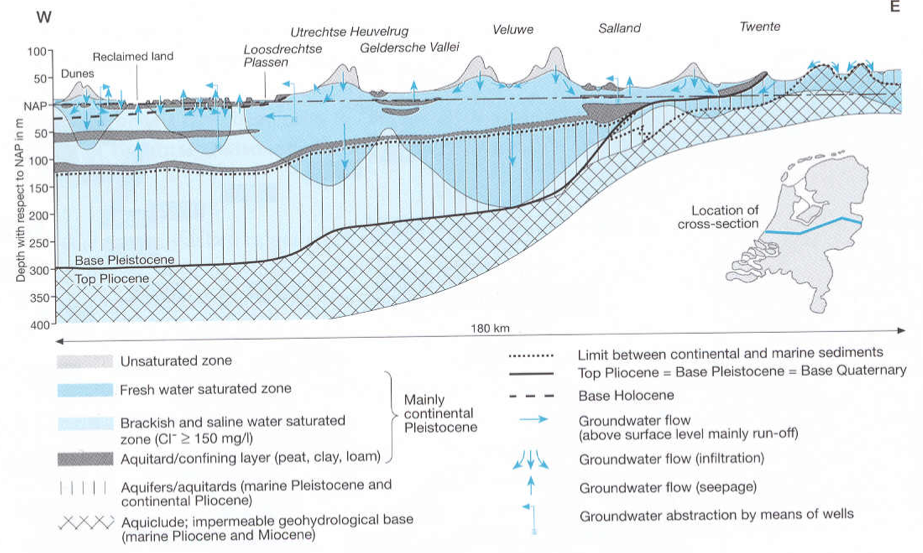
\includegraphics[width=0.8\textwidth]{pictures/floatingFresWaterNLDufour98}
\par\end{centering}
\caption{\label{fig:Dynamically-floating-fresh-water-in-the-Netherlands-cross-section}Dynamically
floating fresh water on salt water in the cross section through the
Netherlands. The interface may take hundreds of years to reach its
equilibrium. It will continuously adapt to changing circumstances
such as climate and sea level rise, as well as to artificial changes
in the water cycle \parencite{DufourF2000}.}
\end{figure}


\section{Questions}
\begin{enumerate}
\item Mention some processes due to which the subsurface may lose water
irreversibly.
\item Explain how these processes work, i.e. what the mechanisms behind
them are, and under which preconditions they occur.
\item Why would one argue that extraction of fresh water from a freshwater
body that floats on salt water is irreversible?
\end{enumerate}

\chapter{\label{chap:Reversible-groundwater-storage}Reversible groundwater
storage}

In the remainder of this syllabus, we will restrict ourselves to reversible
groundwater storage phenomena, i.e. phenomena in which the porous
medium is not changed.

In groundwater flow systems, three separate forms of storage may be
distinguished:
\begin{enumerate}
\item Phreatic storage, which occurs in unconfined aquifers, i.e. aquifers
with a free water table. It is due to filling and emptying of pores
at the top of the saturated zone.
\item Elastic storage, which is due to combined compressibility of the water,
the grains and the porous matrix (soil skeleton). This storage releases
or stores water wherever the pressure changes.
\item Sometimes, the interface between fresh water and another fluid (be
it saline water, oil or gas) can provide a third type of storage.
This works by displacement of the interface, generally between the
fresh water and the saline water. When displacing an interface, the
total volume of water in the subsurface remains essentially the same,
however, the amount of usable fresh water may increase (or decrease)
at the cost of saline water, and therefore, one may consider this
storage of fresh water.
\end{enumerate}

\section{Phreatic storage (water table storage, specific yield, Sy)}

Phreatic storage is due to the filling and emptying of pores above
the saturated zone, i.e. above the water table. Because it is related
to changes of the water table, it is limited to phreatic (unconfined)
aquifers.

The storage coefficient for an unconfined aquifer is called specific
yield and is denoted by the symbol $S_{y}$. It is dimensionless,
as follows from its definition

\begin{equation}
S_{y}=\frac{\partial V_{w}}{\partial h}\label{eq:specific-yield-def}
\end{equation}

where $\partial V_{w}$ is the change of volume of water from a column
of aquifer per unit of surface area and $\partial h$ is the change
of the water table elevation.

$S_{y}$, therefore, is the amount of water released from storage
per square meter of aquifer per m drawdown of the water table.

Hydrogeologists, and groundwater engineers alike, often treat specific
yield as a constant. In reality, the draining and filling of pores
is more complex and this should be kept in mind in order to judge
differences of $S_{y}$ values under different circumstances even
with the same aquifer material. This will be explained further down.

There is no such thing as a sharp boundary between the saturated and
the unsaturated porous medium above and below the water table. In
fact, the water content is continuous across the water table.

\textbf{\emph{The water table is, by definition, the elevation where
the pressure equals atmospheric pressure.}}

Because we relate all pressures relative to atmospheric, we may say
the water table is the elevation where the water pressure is zero
(relative to the pressure of the atmosphere).

The simplest conceptual model for the zone above the water table is
a vertical straw or radius $r$ standing with its open end in water.
Due to adhesion between the water and the straw, the water level will
be sucked upward in the straw against gravity, thereby reaching an
equilibrium height $h$ as shown in figure \ref{fig:Straw-of-radius-r}.

The soil itself may be considered to consist of a dense network of
connected tortuous pores of small but widely varying diameter that
may be fully or partially filled with water. Due to adhesive forces,
pores may even be fully filled above the water table.

\emph{In pores above the water table the pressure is negative (i.e.
below atmospheric).}

If grains can be wetted (attract water), as is generally the case
with water, water will be sucked against gravity, into the pores above
the water table over a certain height. This height mainly depends
on the diameter of the pores.

One can immediately compute the equilibrium of the water in the pore.
We have gravity pulling down the water column reaching above the water
table, and we have the cohesion force. Hence,

\[
\rho gh\pi r^{2}=2\pi r\gamma\cos\left(\alpha\right)
\]
where $\rho$ {[}kg/m $^{3}${]} is the density of water, $g$ {[}N/kg{]}
is gravity, $\gamma$ {[}N/m $^{2}${]} is the cohesion stress, and
$\alpha$ the angle between the cohesion stress and the vertical.
Hence,

\[
h=\frac{2\gamma}{\rho gr}\cos\left(\alpha\right)
\]
which shows that the suction height $h$ is proportional to $1/r$,
the inverse radius of the straw.

In practical situations, $\alpha$ is small so that $\gamma\cos\alpha\approx\gamma$.
As $\gamma$ points is in the direction of the surface tension $\tau$
(see figure  \ref{fig:Straw-of-radius-r}) where the water surface
meets the wall of the straw, we also have

\[
\tau\approx\gamma
\]
with $\tau$ the surface tension of the water surface, which equals
$\tau=75\times10^{-3}\mathrm{N/m}$, see any physical handbook or
look it up on Wikipedia. Therefore, we can compute the suction head
$h$ immediately given a pore radius.

\begin{eqnarray*}
h & \approx & \frac{2\tau}{\rho gr}
\end{eqnarray*}

Numerically,

\begin{eqnarray*}
h & \approx & \frac{150\times10^{-3}}{10^{4}}\frac{1}{r}\\
 & \approx & \frac{1.5\times10^{-5}}{r}\mathrm{\left[m\right]}
\end{eqnarray*}

If we express $h$ and $r$ in mm, (using $h^{*}$ and $r^{*}$ to
indicate mm), we get

\[
h^{*}=\frac{15}{r^{*}}
\]

This implies that water in a pore of 1 mm radius may be sucked up
over about 15 mm, and water in a pore with a radius of 0.1 mm over
15 cm and water in a pore with a radius of 0.01 mm radius over 1.5
m. In reality, the suction may be 50\% smaller because of the angle
$\alpha$ that was ignored here.

\begin{figure}
\begin{centering}
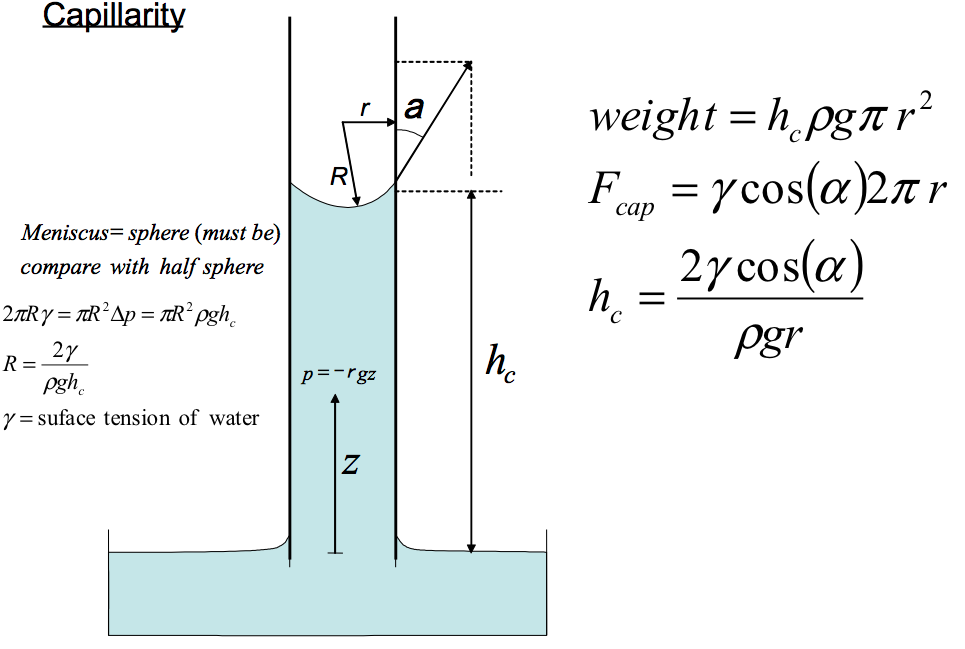
\includegraphics[width=0.6\textwidth]{pictures/capillaryStraw}
\par\end{centering}
\caption{\label{fig:Straw-of-radius-r}Straw of radius $r$ representing a
pore connected to the water table}
\end{figure}

\begin{figure}
\begin{centering}
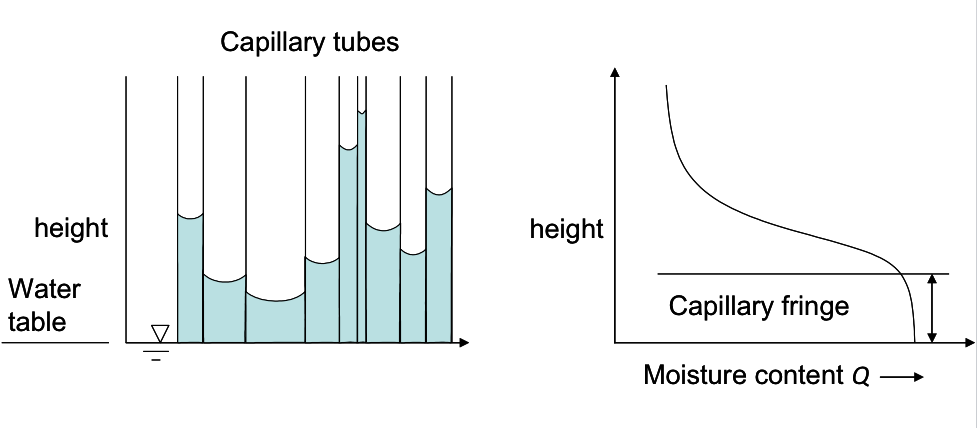
\includegraphics[width=0.8\textwidth]{pictures/capillaryTubes}
\par\end{centering}
\caption{\label{fig:A-porous-medium-as-a-large-set-of-tubes}A porous medium
imagined as a large set of pores of varying diameter}
\end{figure}

A porous medium has pores of varying diameter, which may conceptually
be imagined as in figure \vref{fig:A-porous-medium-as-a-large-set-of-tubes}.
This implies that the line of filled pores will not be sharp. Therefore,
the saturation above the water table will gradually decline as shown
in the right-hand figure .

The diameter of the widest pores will determine the height fully saturated
above the water table, i.e. the thickness of the so-called capillary
fringe. In gravel, the capillary fringe will be almost zero, but it
may be several decimeters or even meters thick in fine-grained materials
such as fine sand, loess, loam and clay. In sands, the capillary zone
is usually 15-30 cm thick, depending on the grain size. The thickness
of the capillary zone is sometimes visible as a wet zone in the banks
of surface water. Note that all water above the water table is under
negative pressure.

\begin{figure}
\begin{centering}
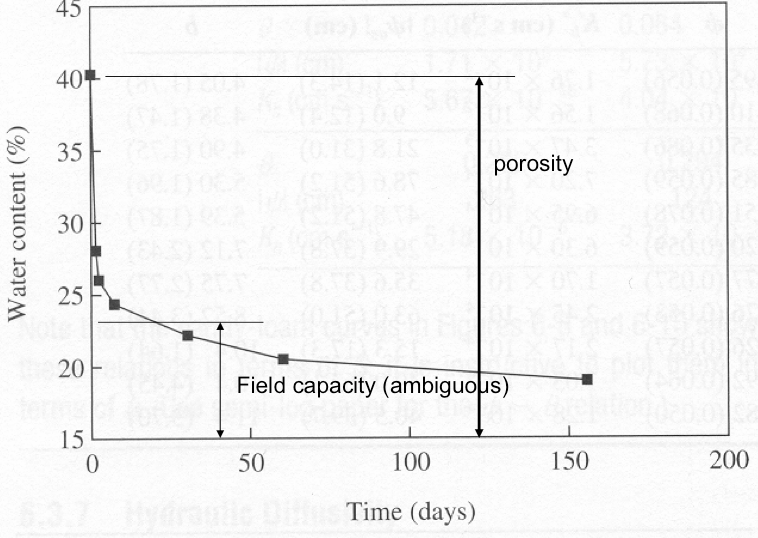
\includegraphics[width=0.6\textwidth]{pictures/drainage-from-column-field-capacity}
\par\end{centering}
\caption{\label{fig:Drainage-of-water-from-column-after-lowering-water-table}Drainage
of water from column after lowering the water table}
\end{figure}

When the water table is lowered, for instance in a column of sand,
and we measure the amount of water drained over time, we see that
drainage is not immediate (figure \ref{fig:Drainage-of-water-from-column-after-lowering-water-table}).
After a couple of days, the drainage rate becomes negligibly small.
We may thus call the amount drained during a couple of days the specific
yield. It is immediately obvious that specific yield is not a unique
physical parameter. The more time we take, the higher the specific
yield becomes. It implies that the duration of the test determines
the value to some extent. It also implies that a specific yield, when
determined from a pumping test of a couple of days duration, is likely
to be smaller than that determined from the seasonal fluctuation of
the water table.

While the amount of water drained from the subsurface due to lowering
of the water table is called\emph{ specific yield}, the amount retained
is the soil is called the\emph{ specific retention}. Together they
add up to the soil's porosity (figure \ref{fig:Relation-between-porosity-specific-yield-and-retention}).\emph{
Specific retention} is essentially the same as the so-called\emph{
field capacity}, i.e. the amount of water the soil can hold against
gravity. It is defined is the amount of water retained in an originally
saturated soil sample after a few days of free drainage at a suction
head of about 200 cm.

\begin{figure}
\begin{centering}
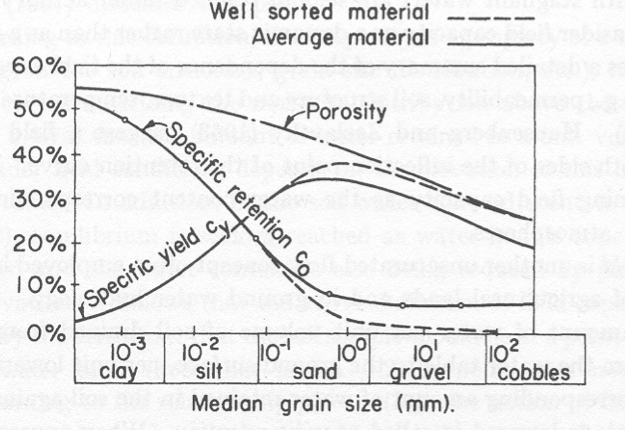
\includegraphics[width=0.6\textwidth]{pictures/porosity-specific-yield-and-retention}
\par\end{centering}
\caption{\label{fig:Relation-between-porosity-specific-yield-and-retention}Relation
between grain size, porosity, specific yield and specific retention
\parencite{Bear1988}.}
\end{figure}

The porosity of porous materials varies, but that of sands is often
about 35\%. Fine sands tend to have somewhat higher values, while
coarse sands tend to have somewhat lower porosities (see figure  \ref{fig:Relation-between-porosity-specific-yield-and-retention}).
This is related to the ease of compaction at the original time of
sedimentation. Smaller grains have a higher surface area and are,
therefore, more difficult to compact. In natural gravels, the pore
space is often filled by finer grains. This reduces the porosity further.
Figure  \ref{fig:Relation-between-porosity-specific-yield-and-retention}
shows that for very fine sands, the specific yield declines despite
the higher porosity. This is mainly due to the higher specific retention
(field capacity) of the finer-grained materials (figure  \ref{fig:Moisture-content-versus-pressure-head})
as well as to the lower hydraulic conductivity of such fine materials,
and, therefore, further reduces their specific yield.

\begin{figure}
\begin{centering}
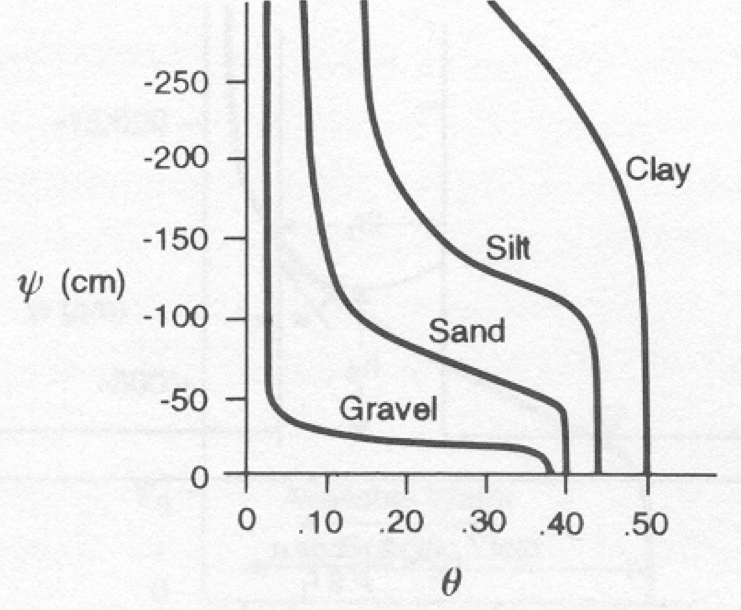
\includegraphics[width=0.6\textwidth]{pictures/moisture-profiles-different-soils}
\par\end{centering}
\caption{\label{fig:Moisture-content-versus-pressure-head}Moisture content
versus pressure head $\Psi$, moisture retention curves \parencite{Bear1988}.}
\end{figure}

The behavior of water in the unsaturated zone is determined largely
by the soil’s moisture retention curve of which a number is sketched
in figure  \ref{fig:Moisture-content-versus-pressure-head} (For the
moisture retention curves of the Dutch soils see \parencite{WoestenJH1994}.

These curves relate the moisture content to suction head, i.e. the
negative head in the pores. Figure  \ref{fig:Moisture-content-versus-pressure-head}
gives the general shape of these curves for typical soil materials.
Therefore, in the case of perfect equilibrium between suction and
gravity, the moisture characteristic curves represent the moisture
content in the soil above the water table. The moisture content at
200 cm suction is generally taken as the field capacity. For sandy
soils, the moisture content at this suction head is a good measure
of the amount of water the soil can hold against gravity under free
drainage conditions.

This implies that the moisture content depends on the distance to
the water table (i.e. the suction). Hence, the ground surface above
a shallow water table tends to be wetter than above a deep water table
under otherwise the same circumstances. This must influence the specific
yield as illustrated in figure \ref{fig:Influence-of-depth-and-time-on-specific-yield}.

\begin{figure}
\begin{centering}
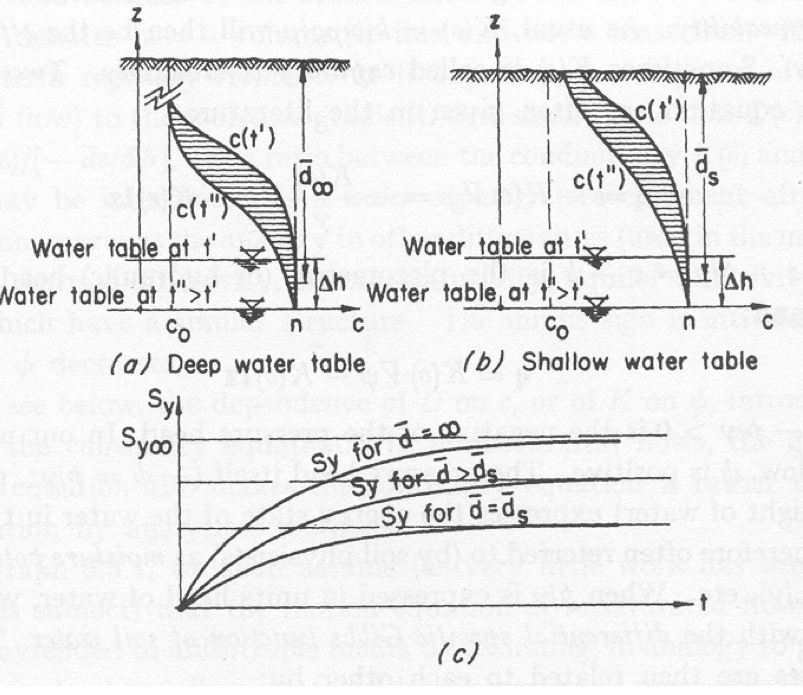
\includegraphics[width=0.8\textwidth]{pictures/shallowMoistureProfilesBear72}
\par\end{centering}
\caption{\label{fig:Influence-of-depth-and-time-on-specific-yield}Influence
of depth and time on specific yield \parencite{Bear1988}.}
\end{figure}

When the water table is lowered, the entire moisture retention curve
is lowered as is shown in figure \ref{fig:Influence-of-depth-and-time-on-specific-yield}-a.
The specific yield times the difference of the two water tables equals
the water from the hatched area times. It demonstrates that the entire
unsaturated profile is involved in the specific yield. As already
mentioned and shown in figure \ref{fig:Influence-of-depth-and-time-on-specific-yield}-c,
specific yield increases with available drainage time.

If the water table is shallow (and the soil material is fine), a major
part of\emph{ the moisture retention curve} will be cut off at ground
surface as is shown in figure \ref{fig:Influence-of-depth-and-time-on-specific-yield}-b.
Lowering of the water table will thus miss a portion of the hatched
area of figure \ref{fig:Influence-of-depth-and-time-on-specific-yield}-a.
Therefore, the specific yield is smaller the shallower the water table
is. This is also shown in figure \ref{fig:Influence-of-depth-and-time-on-specific-yield}-c.

We should thus not be surprised to find that the same fine dune sand
may have a specific yield of 22\% inside a large dune area, where
the water table is usually several meters below ground surface, and
only 8\% in an adjacent flower bulb field with the same sand, but
with a water table of only 60 cm below ground surface.

Soil characteristics may vary between wide limits. Generally, the
coarser the soil, the thinner the capillary fringe (see figure \ref{fig:Moisture-content-versus-pressure-head}).
A complication is that the moisture characteristic curves differ during
wetting and drying. This phenomenon is called hysteresis, but this
is beyond this course.

Groundwater hydrologists dealing with saturated groundwater usually
just use a single constant value for the specific yield in their formulas
and models. The specific yield can be estimated from the soil in question,
from moisture characteristic curves, in the laboratory, from field
measurements, from pumping tests or groundwater-model calibration.

Even though this approach may seem doubtful or just wrong in the eyes
of some, using a constant but appropriately chosen specific yield
works remarkably well in practice. It is more a matter of realizing
oneself when a constant specific yield of a certain value is not applicable.
The above outline is meant as a help in deciding on this and to consciousness
about what is behind this``simple'' hydrologic parameter that we
denote by the symbol $S_{y}$.

Some groundwater models, like MODFLOW, have an option to vary specific
yield automatically with water-table depth.

\subsection{Phreatic responses}

By sensitive continuous measurements of the phreatic head, daily variations
in evapotranspiration can be often determined. While in the past the
groundwater head could be gauged continuously on paper only, modern
head loggers may register the head at short regular intervals and
store large amounts of data internally for later use. With such instruments,
accurate data become widely available and allow more detailed views
on phenomena to be studied and analyzed. Such measurements are already
known from \textcite{ToddD1959} also printed in \textcite{Todd2005}.
figure \ref{fig:water-table-fluctuation-due-to-evapotranspiration}
shows the daily fluctuation of the water table due to daily evapotranspiration
measured more than sixty years ago. However, we find such fluctuations
in all frequent registrations of shallow water tables under summer
circumstances.

\begin{figure}
\begin{centering}
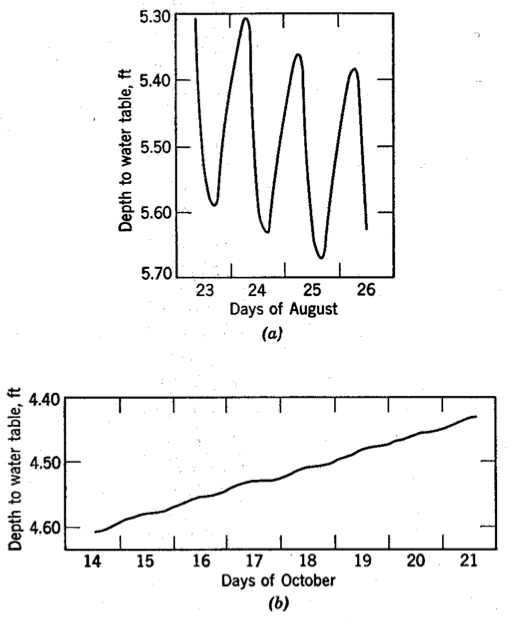
\includegraphics[width=0.5\textwidth]{pictures/effTranspirationOnWaterTable}
\par\end{centering}
\caption{\label{fig:water-table-fluctuation-due-to-evapotranspiration}Measured
water-table fluctuations due to evapotranspiration variations \parencite{Todd2005}.}
\end{figure}

\begin{figure}
\begin{centering}
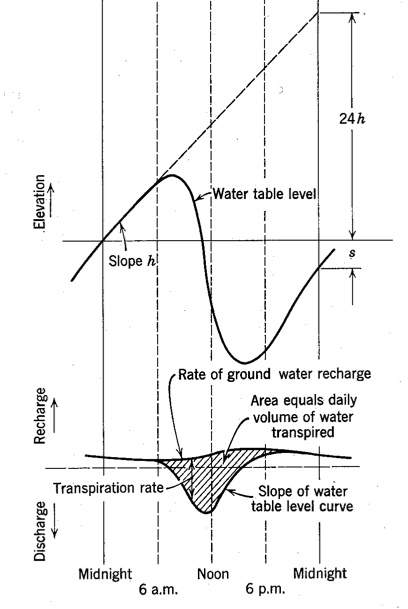
\includegraphics[width=0.5\textwidth]{pictures/watertabelRechargeTranspiration}
\par\end{centering}
\caption{\label{fig:Determining-the-evapotranspiration-from-water-table-response}Determining
the evapotranspiration from water-table variations and a given specific
yield \parencite{Todd2005}.}
\end{figure}

If the specific yield is known, evapotranspiration rates can sometimes
be determined from such water-table registration. This can be demonstrated
on the hand of these old measurements (figure \ref{fig:water-table-fluctuation-due-to-evapotranspiration}
and figure \ref{fig:Determining-the-evapotranspiration-from-water-table-response}).
The groundwater balance at this point may be expressed as

\[
\overline{N}+N\left(t\right)=S_{y}\frac{\partial\phi}{\partial t}
\]
where $\overline{N}$ is the long-term trend of the net water-table
recharge (positive or negative, i.e. precipitation minus evapotranspiration
from the water table). $N\left(t\right)$ is the short-term variation
(during the day). So if one plots the derivative of the water table
in a point versus time, it may be split into a more or less constant
(long-term) trend and a the remainder due to short-term (daily) variation.
If this short-term variation can be attributed to evapotranspiration
from the water table, as it obviously is the case in the figure ,
one may determine it by taking the surface area between the measured
head curve and its long-term trend, multiplied by the specific yield
(hatched surface in figure \ref{fig:Determining-the-evapotranspiration-from-water-table-response}\label{fig:water-table-fluctuation-due-to-evapotranspiration-1}).

\subsection{Questions}
\begin{enumerate}
\item What is the dimension of specific yield? What is the dimension of
the elastic storage coefficient. What is the dimension of the specific
storage coefficient?
\item How do specific retention, specific yield and porosity relate to each
other?
\item How does porosity relate to grain size in general, and what is the
reason?
\item Given another term for specific retention, one that is generally using
in agriculture.
\item How does specific retention relate to grain size?
\item If the water table is lowered, which water is released around or above
the water table?
\item What is the definition of the unsaturated zone?
\item Is it likely that the water from a rain shower easily infiltrates
through worm and rabbit holes? If so explain why. If not also explain
why?
\item What is a probable value for specific yield in a sand with porosity
of 35\%? And why?
\item How does capillary zone relate to air-entry pressure?
\item What is actually measured with the air-entry pressure?
\item How does the specific yield relate to the depth of the water table?
\item Using the model of a straw, how does capillary rise relate to the
straw radius and the water surface tension?
\item Given a grain diameter of 0.2 mm, a radius that is 1/7th of this radius,
and a water surface tension $\gamma=75\times10^{-3}\mathrm{N/m}$,
what would be the capillarity rise if the angle of the water surface
and the straw is assumed to be zero?
\end{enumerate}
\pagebreak{}

\section{\label{sec:Elastic-Storage}Elastic Storage}

\subsection{Introduction}

Till now, we only considered storage at the water table and gave very
simple, but practical examples largely ignoring spatial dimensions.
Spatial dimensions will be dealt with later. In this section, we handle
the physics of elastic storage and will give some interesting everyday
examples that are sometimes easily overlooked.

Elastic storage is the only storage occurring in confined and semi-confined
aquifers, i.e. in aquifers without a water table, meaning aquifers
that are completely filled with water from floor to ceiling. In such
aquifers, we have no lowering of the water table whatsoever, unless
the head is lowered to beneath the ceiling of the aquifer, a case
further ignored here.

Therefore, in confined aquifer storage can only result from compression
of the water and depression of the aquifer. The compressibility of
the water and the grains themselves is quite obvious, but often the
less obvious storage is the most important part. This is the deformation
of the soil skeleton, the bulk matrix or the (bulk) porous medium
as it is called.

\subsection{Loading efficiency}

To analyze the physics of elastic storage, we start with noting that
the total load at any depth is carried by the total (vertical pressure)
$\sigma_{z}$ or $p\,\mathrm{N/m^{2}}$. This total pressure must
equal the sum of the vertical grain pressure (the so-called effective
stress, $\sigma_{e}$) and the water pressure $\sigma_{w}$

\[
p=\sigma_{e}+\sigma_{w}
\]

This is indicated in figure \ref{fig:The-weight-of-ground-supported-by-sigmaw+sigmae}.
The brown horizontal beams and the springs in this figure  are imaginary;
they replace the volume $V_{0}$ ( $1\mathrm{m^{3}}$ say) that has
been cut out of the aquifer. The two imaginary springs have the same
properties as the water and the porous medium respectively. Let us
see what happens when the pressure is increased by $\Delta p$.

In that case, the volume (or height) $V_{0}$ is reduced by $\Delta V$
and the springs pressures are increased by $\Delta\sigma_{w}$and
$\Delta\sigma_{e}$ respectively. The springs have a different stiffness,
so $\Delta\sigma_{w}\ne\Delta\sigma_{e}$. However, each string will
always carry a fixed proportion of the total stress. Therefore, we
may write

\[
\Delta\sigma_{w}=LE\,\Delta p
\]
where $LE$ is this fixed proportion and is called the\emph{ loading
efficiency}. The $LE$ must obviously lie between $0$ and 1 and is
fixed for any particular porous medium. So if we put a weight, like
a layer of sand, on ground surface, $p$ in figure \ref{fig:The-weight-of-ground-supported-by-sigmaw+sigmae}
will increase by $\Delta p$, a change that is equal to the weight
of the layer of sand per $\mathrm{m}^{2}$ placed on ground surface.
We may then say $\Delta\sigma_{w}=LE\,\Delta p$, where the loading
efficiency $LE$ is a fixed number between 0 and 1, specific to a
aquifer in question. If we have a piezometer in the aquifer, we'll
notice that the water level (hence, the head) has risen by placing
the sand on ground surface. The head rise is given by

\[
\Delta\phi=\frac{LE}{\rho g}\Delta p
\]

Now assume that $\Delta p$ is not due to a layer of sand placed on
ground surface, but due to a change of the barometer pressure as in
figure \ref{fig:LE-BE-barometer}. Then the same reasoning applies,
because the subsoil cannot know the difference between a pressure
change due to a layer of sand placed on ground surface or due to an
equivalent rise of the barometer pressue.

\begin{figure}
\begin{centering}
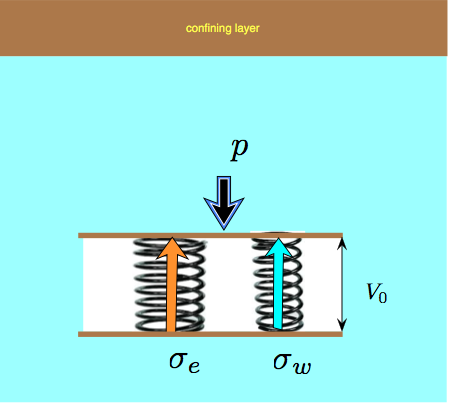
\includegraphics[width=0.6\textwidth]{pictures/CompressionTwoSprings}
\par\end{centering}
\caption{\label{fig:The-weight-of-ground-supported-by-sigmaw+sigmae}The weight
of the ground plus water is supported by two pressures, the water
pressure $\sigma_{w}$ and the effective pressure $\sigma_{e}$}
\end{figure}

\begin{figure}
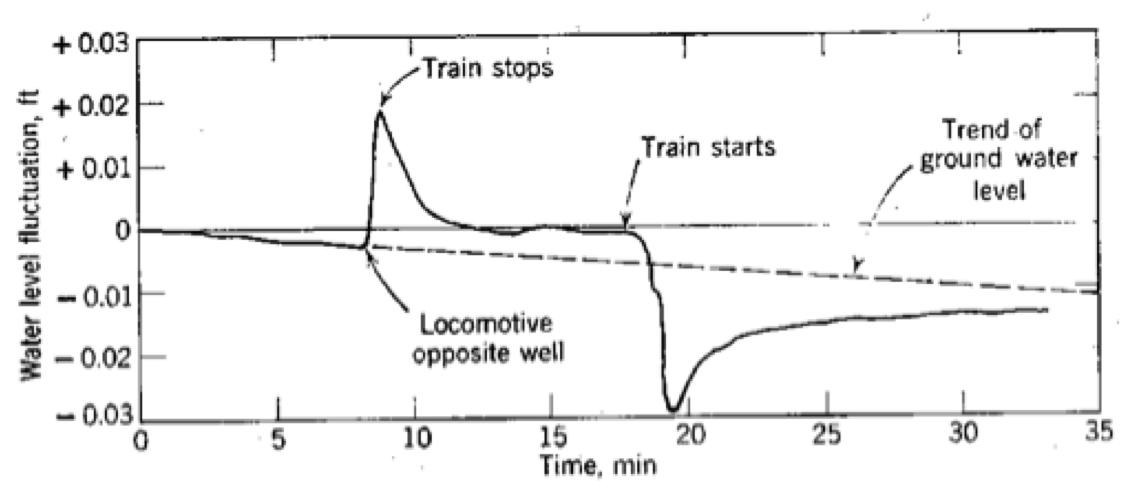
\includegraphics[width=0.6\textwidth]{pictures/todd_train}

\caption{\label{fig:ToddsTrain}Water level fluctuation in a confined aquifer
produced by a train stopping near an observation well \parencite{ToddD1959,Todd2005}}
\end{figure}

A nice and famous early example of loading efficiency is the impact
of a train stopping at a station and leaving again some time later
(figure \ref{fig:ToddsTrain}). The weight of the locomotive compresses
the aquifer a bit, thus reducing its pore space. This in turn compresses
the groundwater, which cannot readily escape. Hence, its pressure
rises and it starts to flow sidewards, so that the pressure gradually
decreases towards its original trend. When the train leaves, the opposite
occurs. The removal of the load reduces the effective stress, which
causes the aquifer to bounce back, providing more pore space to the
water, which depressurizes and increases somewhat in volume. This
reduced water pressure causes surrounding groundwater to flow inward
to fill up the gap due to which the pressure gradually normalizes.
\begin{verse}
\emph{Q: Think of another way for the water to escape from a semi-confined
aquifer.}
\end{verse}

\subsection{Barometer efficiency}

figure \ref{fig:LE-BE-barometer} left shows the situation where the
pressure increase is caused by a load (of sand) on ground surface;
the right-hand picture shows how the same pressure increase is caused
by an increase of the barometer pressure. The question is, how does
the change of the barometer pressure alter the head (water level)
in the piezometer?

\begin{figure}
\begin{centering}
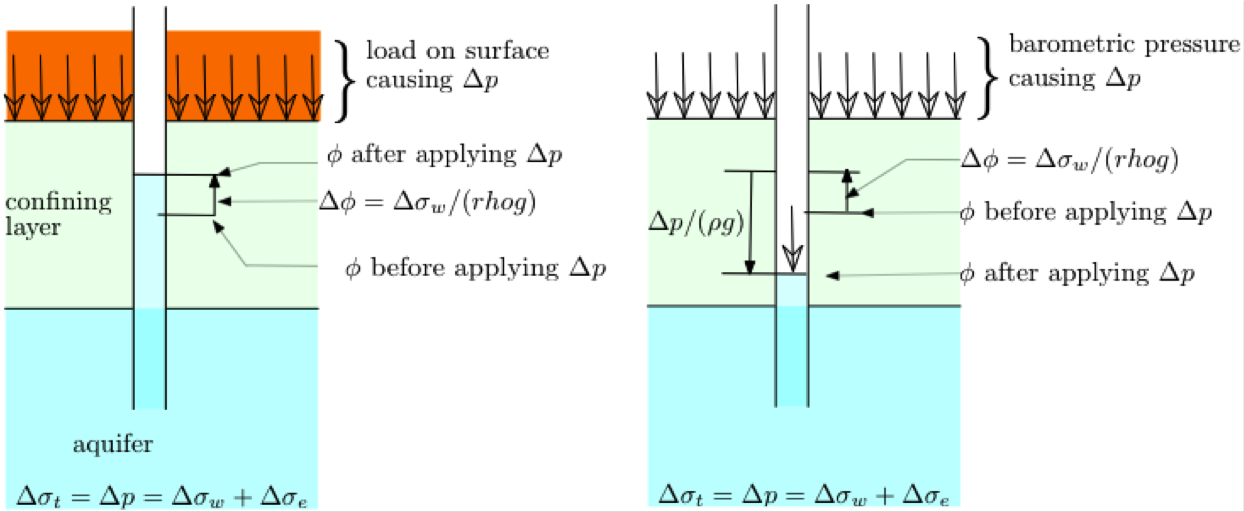
\includegraphics[width=0.8\textwidth]{pictures/Load_barometer}
\par\end{centering}
\centering{}\caption{\label{fig:LE-BE-barometer}Effect on head in confined aquifer by
a load $\Delta p$ on surface versus an increase of the barometric
pressure.}
\end{figure}

As said above, for the pressure in the aquifer there is no difference
between the two pictures. However, there is a difference between the
head (i.e. the water level) in the piezometer in the left picture
and in that of the right picture. When placing a layer of sand on
ground surface, the pressure on the water surface in the piezometer
does not change. However, when the the barometer pressure changes,
the pressure on the water surface in the piezometer does change. That
change is, of course, exactly equal to the change of the barometer
pressure. To see how the head changes due to a change of the barometer
pressure let us just write out the water pressure at the bottom of
the piezometer. It is clear that this pressure changes due to the
change at ground surface such that $\Delta a=\Delta p$, with $\Delta a$
the change of the barometer pressure.

Now assume that the head (i.e. the water level) in the piezometer
changes by an amount $\Delta\phi$. The change of the water pressure
at the bottom of the piezometer then is

\[
\Delta\sigma_{w}=\rho g\Delta\phi+\Delta a
\]
But we already know the change of the water pressure

\[
\Delta\sigma_{w}=LE\,\Delta a
\]
Hence,

\[
\rho g\Delta\phi+\Delta a=LE\,\Delta a
\]
and so

\begin{align*}
\rho g\Delta\phi & =-(1-LE)\,\Delta a\\
 & =-BE\,\Delta a
\end{align*}
where $1-LE$ is called the\emph{ barometer efficiency}, $BE$. Just
like the loading efficiency, the barometer efficiency varies between
0 and 1.

The minus sign indicates that the head in the piezometer declines
when the barometer goes up. This should be obvious as the the water
pressure increases by $LE\,\Delta a$ which is a fraction of the barometer
pressure, which would cause the water level in the piezometer to rise,
but at the same time the full barometer pressure pushes on the water
table in the piezometer, which causes the water level to decline accordingly.
Together, the net effect is a decline of the head in the piezometer
by $BE\,\Delta a$, a fraction of the barometer pressure change.

From the equivalence of the previous equation couple, it follows that

\[
BE+LE=1
\]

\begin{figure}
\begin{centering}
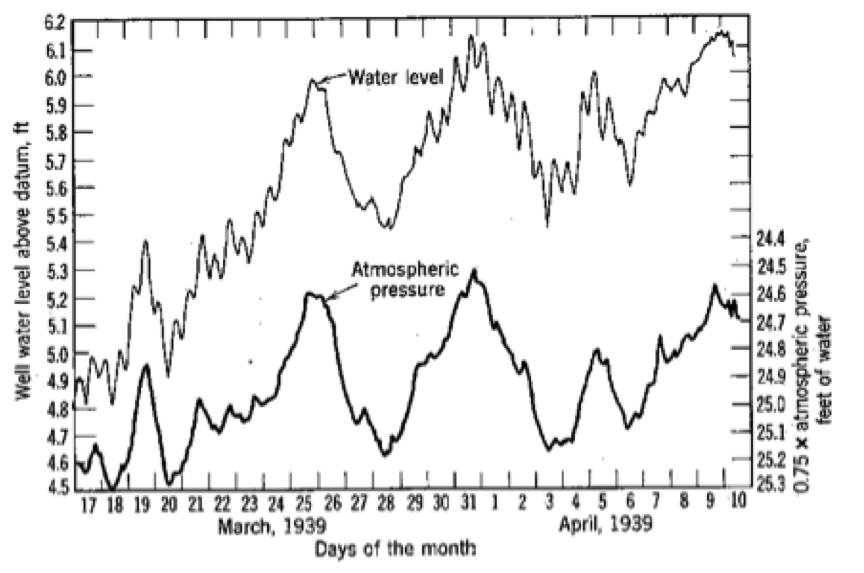
\includegraphics[width=0.6\textwidth]{pictures/ToddBarometerGraph}
\par\end{centering}
\caption{\label{fig:Todd-baro-graph}Example of a high degree (75\%) of barometric
efficiency \parencite{ToddD1959,Todd2005}. It shows the response
of the head in a well penetrating a confined aquifer together with
the barometric pressure. Note that the axes on the right is reversed
to show the similarity of the two curves (head down when barometer
pressure goes up and vice versa).}
\end{figure}

A famous example of the barometer efficiency was given by \parencite{ToddD1959,Todd2005},
figure \ref{fig:Todd-baro-graph}. This example is used here because
it is famous as one of the first-ever published. However, barometer
effects are always seen in piezometers in confined aquifers. The barometer
efficiency generally varies between 20\% and 80\%.

The barometer influence causes a normally observed noisy behavior
of the head time series from confined and semi-confined aquifers.
This noisy behavior occurs also when groundwater is in perfect rest.
Barometer pressure fluctuations do affect both the head measured in
piezometers as the pressure measured in pressure gauges. Only if heads
are measured at short time intervals of hours rather than weeks, would
the noisy behavior of the head in confined aquifers actually show
its clear one-to-one relation with the course of the barometer pressure.
Therefore, such a noisy time series behavior actually shows that a
piezometer is in a (semi-)confined aquifer. Unless we have very thick
unsaturated zones with substantial resistance against air flow, we
will not see much if any barometer fluctuation in water-table aquifers
\parencite{RasmussenT1997}.

\subsection{How much are the loading efficiency and the barometer efficiency
when expressed in the properties of the water and the porous medium
?}

If the total pressure $p$ is increased by $\Delta p$, the porous
medium is compressed together with the water that it contains. Clearly,
the increase of the water pressure will also compress the individual
grains. However, sand grains are about 50 times less compressible
than water. Therefore, the effect of the grains being compressed themselves
can be safely neglected.

On the other hand, the porous medium (the skeleton of grains) itself
is far less stiff than the grains themselves. The porous medium is
essentially compressed due to some deformation of the grains at the
expense of the porosity of the medium. In fact, as it turns out, the
compressibility of the porous medium is of the same order of magnitude
as that of the water, so they must both be taken into account.

\begin{figure}
\begin{centering}
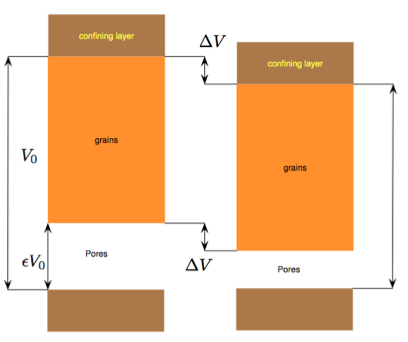
\includegraphics[width=0.6\textwidth]{pictures/compressionAquifer}
\par\end{centering}
\caption{\label{fig:Compression-of-the-porous-medium}Compression of the porous
medium, while the volume of the grains remains unchanged because their
compressibility is negligible compared to that of both the water and
the porous medium.}
\end{figure}

Hence, the volume $V_{0}$ is compressed by $\Delta V$ when the pressure
$p$ is increased by $\Delta p$.

Assume the aquifer to be of infinite lateral extent, so that the only
possible compression is downward. This implies that $\Delta V=\Delta H$,
which is the change of the thickness of the considered part of the
layer that we replaced by the springs in figure \ref{fig:The-weight-of-ground-supported-by-sigmaw+sigmae}.
Hence, both springs underlie the same compression $\Delta H$.

Let the water have a compressibility $\alpha$ meaning that a $m^{3}$
of water would be compressed by the fraction $\alpha$ for each increase
of the water pressure by $1\,\mathrm{N/m^{2}}$. Similarly, let the
porous medium have a compressibility of $\beta,$ meaning that one
$m^{3}$ of the porous medium would be compressed by the factor $\beta$
for each $\mathrm{N/m^{2}}$ increase of effective stress, $\sigma_{e}$.
These compressibilities, therefore, have dimension $\mathrm{m^{3}/m^{3}/\left(N/m^{2}\right)}=\mathrm{m^{2}/N}$.

Now consider that the soil was put under an extra total pressure of
$\Delta p$ causing it to be compressed by the fraction $\Delta H/H_{0}=\Delta V/V_{0}$.
Then the effective pressure increases due to this compression $\Delta H$
by

\[
\Delta\sigma_{e}=-\frac{\Delta V/V_{0}}{\beta}
\]

Because the grains are considered incompressible, it follows that
the change of pore volume equals the change of the total volume. Therefore,
for the water we have a relative volume change (= compression) of
$\Delta V$ per $\epsilon V_{0}$. Therefore, the water pressure increase
is

\begin{eqnarray*}
\Delta\sigma_{w} & = & \frac{\Delta V/\left(\epsilon V_{0}\right)}{\alpha}\\
 & = & \frac{\Delta V/V_{0}}{\epsilon\alpha}
\end{eqnarray*}

Because we have now related both $\Delta\sigma_{w}$ and $\Delta\sigma_{w}$
to the relative volume change $\Delta V/V_{0}$, we also know the
ratio between the change of the effective pressure and the water pressure

\begin{eqnarray*}
\frac{\Delta\sigma_{e}}{\Delta\sigma_{w}} & = & \frac{\epsilon\alpha}{\beta}
\end{eqnarray*}
and so

\begin{eqnarray*}
\Delta\sigma_{e} & = & \frac{\epsilon\alpha}{\beta}\Delta\sigma_{w}
\end{eqnarray*}
With this, we can eliminate $\Delta\sigma_{e}$ from the pressure
equation:

\begin{eqnarray*}
\Delta p & = & \Delta\sigma_{w}+\Delta\sigma_{e}
\end{eqnarray*}
to obtain

\[
\Delta p=\left(1+\frac{\epsilon\alpha}{\beta}\right)\Delta\sigma_{w}
\]
And because $\Delta\sigma_{w}/\Delta p=LE$ we have

\[
LE=\frac{\beta}{\beta+\epsilon\alpha}
\]
And because $BE=1-LE$ we also have

\[
BE=\frac{\epsilon\alpha}{\beta+\epsilon\alpha}
\]


\subsection{Specific (elastic) storage coefficient}

The specific storage coefficient is the change of volume per unit
volume of space per unit change of head:

\begin{equation}
S_{s}=-\frac{\partial V/V_{0}}{\partial\phi}\label{eq:Ss-definition}
\end{equation}
it is the volume of water released from the porous medium per m of
lowering of the head $\phi$ (a negative $\Delta\phi$ yields a positive
amount of water). It is also immediately clear that the dimension
of $S_{s}$ is $\mathrm{\left[m^{3}/m^{3}\right]/m=m^{-1}}$, the
volume of water released per $\mbox{m}^{3}$ of the porous medium
per m of head decline.

Now consider the situation in which we lower the water pressure, for
instance by extracting water from the aquifer. Lowering of the water
pressure in no way changes the total pressure. Therefore, $\Delta p=0$,
which yields

\begin{equation}
0=\Delta\sigma_{w}+\Delta\sigma_{e}\label{eq:deltaSigma_w+deltaSigma_e=00003D0}
\end{equation}

However, the amount of water squeezed out of the porous medium changes.
A lowering of head causes an increase of the effective pressure (grain
pressure), and, hence, is associated with a compression of the porous
medium. Therefore, an increase of the effective pressure ( $\Delta\sigma_{e}>0$),
reduces the pore volume by $\Delta V$ due to which the same volume
of water is squeezed from the porous medium

\[
\Delta V_{pm}=+V_{0}\beta\Delta\sigma_{e}
\]
where $pm$ means ''porous medium ''.

An increase of the water pressure, would cause a compression of the
water within the pores $\epsilon V_{0}$, by

\[
\Delta V_{w}=-\alpha\left(\epsilon V_{0}\right)\Delta\sigma_{w}
\]

The total amount of water released equals the volume squeezed out
due to the reduction of the pore space plus the volume that is generated
by expansion of the water due to the reduction of the water pressure:

\begin{eqnarray*}
\Delta V & = & -\alpha\left(\epsilon V_{0}\right)\Delta\sigma_{w}+V_{0}\beta\Delta\sigma_{e}
\end{eqnarray*}
and because $\Delta\sigma_{e}=-\Delta\sigma_{w}$ in this case (see
equation \ref{eq:deltaSigma_w+deltaSigma_e=00003D0}), we have

\[
\frac{\Delta V}{V_{0}}=-\left(\alpha\epsilon+\beta\right)\Delta\sigma_{w}
\]
so that

\[
\frac{\Delta V/V_{0}}{\Delta\sigma_{w}}=-\left(\epsilon\alpha+\beta\right)
\]
now with $\Delta\sigma_{w}=\rho g\Delta\phi$ get \ref{fig:Van-der-Gun-specific-storage}
\begin{eqnarray}
\frac{\Delta V/V_{0}}{\rho g\Delta\phi} & =- & \left(\epsilon\alpha+\beta\right)\label{eq:specific-storage-from-soil-and-water-stiffness}
\end{eqnarray}

and, therefore

\[
\frac{\Delta V/V_{0}}{\Delta\phi}=-\rho g\left(\epsilon\alpha+\beta\right)
\]

so that with $S_{s}=-\frac{\Delta V/V_{0}}{\Delta\phi}$, we now have
a formula that allows us to compute the specific elastic storage coefficient
to the physical elastic properties of the aquifer, $\beta$, and the
water, $\alpha$.

\begin{equation}
S_{s}=\rho g\left(\epsilon\alpha+\beta\right)\label{eq:specific-storage-as-rho-g-times(epsAlpha+beta)}
\end{equation}
which, considering that we reduce the $\Delta$ to the infinitesimally
small $\partial$, completes the proof (see equation \ref{eq:Ss-definition}).

Notice the dimension of $S$

\[
\mbox{dimension of }S_{s}=\mathrm{\left[\frac{kg}{m^{3}}\right]\left[\frac{N}{kg}\right]\left[\frac{m^{2}}{N}\right]}=\mathrm{\left[\frac{1}{m}\right]}
\]

As often is more practical to write the dimension of gravity $g$
as $\mathrm{\left[\frac{N}{kg}\right]}$ instead of $\mathrm{\left[\frac{m}{s^{2}}\right]}$.
They are the same, the first can be seen as the force in $N$ by which
gravity pulls a mass of 1 kg downward; the second as the acceleration
a mass of 1 kg would undergo when freely left to gravity to fall.

\subsection{Application (not for exam)}

The compressibility of water is

\begin{eqnarray*}
\alpha & = & -\frac{1}{V_{w,0}}\frac{\partial V_{w}}{\partial\sigma_{w}}\,\mathrm{\mathrm{\left[L^{2}/F\right]^{2}}}
\end{eqnarray*}

where $\alpha\approx4.4\times10^{10}\,\mathrm{m^{2}/N}$. Clearly,
$\partial V_{w}/V_{w,0}$ is the relative change of the water volume.
There is some dependency on dissolved components, water containing
dissolved gas, may be up to three times more compressible than water
without dissolved gas under normal pore pressure (Lyons, William C.
(2010): Working Guide to Reservoir Engineering; Elsevier).

The compressibility of the porous medium is

\[
\beta=-\frac{1}{V_{T,0}}\frac{\partial V_{T}}{\partial\sigma_{e}}
\]
where $\partial V_{T}/V_{T,0}$ is the relative change of the volume
of the porous medium. $V_{T}$ is, the total volume of the considered
soil (including its pores). $\sigma_{e}$ is the effective stress
(=grain pressure), i.e. that part of the total stress, $p$, that
is not carried by the water pressure $\sigma_{w}$. The total pressure
equals the weight of the overburden, i.e. that of the overlying formations
including the water that they contain. Hence $\sigma_{e}=p-\sigma_{w}$.

The soil compressibility $\beta$ is the gradient of a stress-strain
curve (relative volume change as a function of effective stress) of
a dry soil sample put under increased stress in the laboratory, such
that side-ward movement is prevented, exactly as it is the case in
the actual aquifer under uniform vertical stress. Unlike water, the
compressibility of soil is not necessarily a constant. If the soil
is put under higher stress than it had ever supported before, then
it consolidates, meaning that the change of volume is largely irreversible.
But under lower than historic stresses, a constant compressibility
can be determined, and truly elastic behavior can be assumed. It should
be clear, that this compressibility depends on porosity.

\textcite{Gun1980} presented the following relationship between the
compressibility of aquifers and depth based on laboratory measurements
that were carried out by Van der Knaap (1959, unfortunately no direct
reference).

\begin{equation}
\beta=\epsilon\left(3\times10^{-11}+6.6\times10^{-11}z^{-0.7}\right)\label{eq:Van-der-Knaap-aquifer-skeleton-compressibility}
\end{equation}
where $z$ in {[}km{]} is the depth below ground surface and $\epsilon$
is porosity. Then we can apply equation \ref{eq:specific-storage-as-rho-g-times(epsAlpha+beta)}

\[
S_{s}=\rho g\left(\epsilon\alpha+\beta\right)
\]

With the relation of \textcite{Gun1980}, we obtain the graphs shown
in figure \ref{fig:Van-der-Gun-specific-storage}. As can be concluded
from the graph, values in the order of $10^{-5}\,\mathrm{Pa^{-1}}$
are often found in practice, where we generally have porosities of
around 35\% in fluviatile and eolian sandy aquifers.
\begin{verse}
\emph{Question}: Is it feasible that compressibility of the porous
medium is proportional to porosity?
\end{verse}
\begin{figure}
\begin{centering}
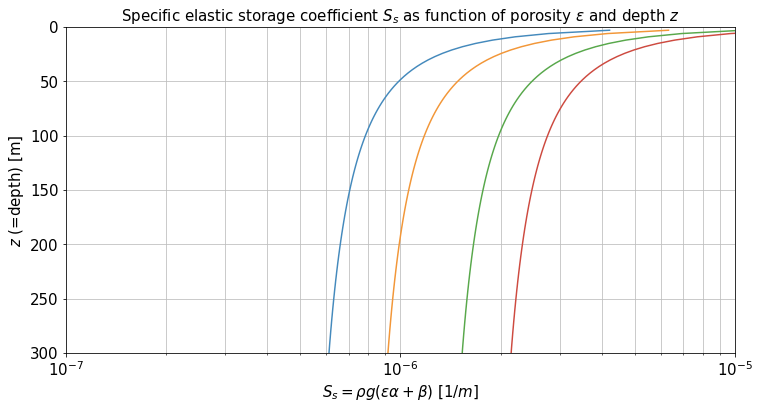
\includegraphics[width=0.8\textwidth]{pictures/SsVdGun1980}
\par\end{centering}
\caption{\label{fig:Van-der-Gun-specific-storage}Computed specific storage
coefficient $Ss=\rho g\left(\epsilon\alpha+\beta\right)\,\mathrm{\left[m^{-1}\right]}$
as a function of depth below ground surface using the relation by
\textcite{Gun1980}.}
\end{figure}


\subsection{Questions}
\begin{enumerate}
\item Explain what loading efficiency is.
\item What factors contribute to the elastic storage coefficient and what
factor may be neglected?
\item If a load $\Delta p$ is placed on top of a confined aquifer and the
water pressure in the aquifer is increased to $\Delta\sigma_{w}=LE\,\Delta p$,
then how much does the head change in a piezometer in that aquifer?
\item The same question for the situation where $\Delta p$ is caused by
an increase of the barometer pressure.
\item Assume we have a pressure gauge (often also called pressure transducer
or pressure sensor) in a piezometer in the confined aquifer that measures
the absolute pressure (i.e. the atmospheric pressure + the water pressure).
On day 1, the barometer rises by $\Delta p$ and is constant thereafter.
Later, a load $\Delta p$ is placed on ground surface. What is the
difference, if any, in the registration done by the pressure gauge
in the piezometer, and what is the difference with the hand-measured
head in the piezometer?
\item The measurements by pressure gauges in confined and semi-confined
aquifers are corrected for barometer pressure changes by subtracting
the barometer pressure from the measured pressure. Does this mean
that the fluctuations of the barometer pressure are eliminated by
this correction? If so, explain why. If not, also explain why.
\item What is actually the result of this correction of the registered pressures?
What actually do we get by this correction?
\item How can we compute the specific elastic storage coefficient $S_{s}$
from the measured barometric efficiency? Note:\\
 
\begin{eqnarray*}
BE & = & 1-\frac{\beta}{\epsilon\alpha+\beta}\\
Sy & = & \rho g\left(\epsilon\alpha+\beta\right)
\end{eqnarray*}
\item Think of what we can easily estimate and what we know, respectively
what we don't know? Assume that porosity $\epsilon$ can be reasonably
well estimated.
\item Consider a confined aquifer and the following two situations. First
there is a loading at ground surface with value $\Delta p$. The head
is measured both in a piezometer and in a pressure gauge (which measures
the absolute water pressure in the aquifer). What is the difference
between the two measurements?
\item In the same location, consider an increase of the barometer pressure
that is of the same magnitude as the surface loading $\Delta p$ before,
so $\Delta a=\Delta p$. What is the difference in the head measured
with a piezometer and that measured with a pressure gauge?
\item What is the difference between the heads measured with the piezometer
in the two cases?
\item What is the difference between the pressures measured with the pressure
gauges in the two cases?
\item How much is the barometer effect in an unconfined aquifer?
\item How will the head or pressure in a piezometer in a semi-confined aquifer
after a uniform surface load was put on the ground surface? Think
of compression and leakage through the overlying aquitard.
\item What aquifer parameter might we derive from this behavior? Think of
the leakage.
\item With two pressure transducers, one measuring the barometer pressure
and the other the water pressure in some piezometer in a confined
aquifer, how can we compute the barometer efficiency? What parameter
do we still miss to obtain true numerical values?
\item How does the head in a water-table aquifer react to barometer fluctuations?
\item How large may the variation of the head due to barometer fluctuations
become given a range of atmospheric pressure from variation between
970 to 1040 mbar (=cm head)?
\item What values do you expect for total elastic storage coefficients of
aquifers in practice?
\item How could we measure the elastic storage coefficient in a confined
aquifer below the sea bottom?
\item Does the value of the specific yield that we may derive from barometer
efficiency, water storativity and porosity refer to the value of the
measuring point or to the thickness of the entire aquifer?
\item How useful is it to measure local porosity at the screen position
of the piezometer to compute the storage coefficient of the aquifer?
\end{enumerate}

\section{\label{sec:Earth-tides}Earth tides (not for exam)}

Even far from the ocean and even after correcting for varying barometer
pressures, the groundwater head in confined aquifers may show a response
that closely resembles tides. This fluctuation matches the passage
of the sun and the moon due to a rotating earth, exactly like it is
the case with sea tides, (\parencite{ToddD1959,Todd2005,BoemenPJT1989}),
figure \ref{fig:Earth-tides}.

\begin{figure}
\begin{centering}
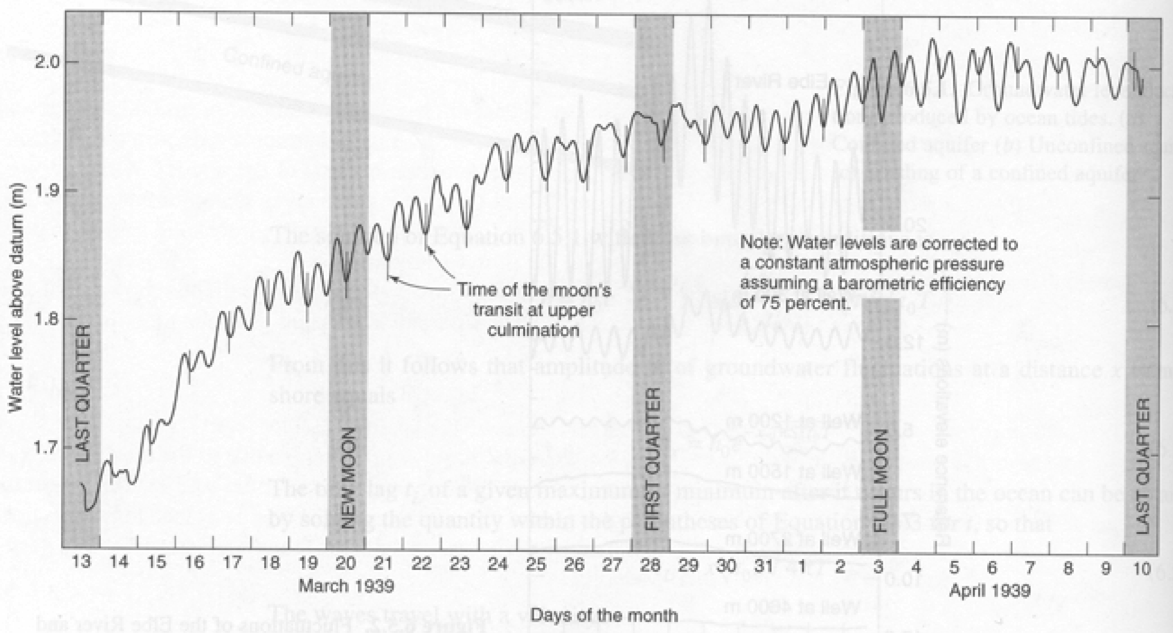
\includegraphics[width=0.8\textwidth]{pictures/earthTides}
\par\end{centering}
\caption{\label{fig:Earth-tides}Water level fluctuations in a confined aquifer
produced by earth tides (from \textcite{ToddD1959,Todd2005})}
\end{figure}

Like normal tides, earth tides are an indirect consequence such gravity
variations. It can be shown that they are caused as an indirect effect
of the deformation of the earth's mantle on which the stiff crust
floats. A bulge is formed by the mantle by the attraction of the sun
and the moon. The earth crust itself is so thin compared to the earth
mantle that it behaves like a thin hard sheet floating on the mantle
and is stretched by the mantle as it bulges out under tidal attraction.
During stretching, porosity increases and the head lowers. When the
stretching is released, the opposite occurs as is shown in equation
\ref{fig:Earth-tides}.

This variation may be estimated with up to 50\% accuracy from solid
earth-tide theory \parencite{Kamp1983}. The dilatation (stretching)
is more or less fixed due to the relation with the mantle, but different,
for any point on earth. According to \textcite{BredehoeftJ1967} it
is about

\[
\Delta\phi\approx\frac{10^{-8}}{S_{s}}
\]
at moderate latitudes. Using this number, one may relate the expected
magnitude of the water-level fluctuations directly to the specific
storage coefficient. With $S_{s}$ in the order of $10^{-6}$/m for
sandstones and $10^{-7}$/m for granites, a fluctuation amplitude
of 1 to 10 cm may be expected.

A thorough analysis of earth tides is beyond the scope of this course.
There is a wealth of literature on the subject; a good quantitative
paper is \textcite{Kamp1983}.

\chapter{\label{chap:One-dimensional-transient-flow}One-dimensional transient
groundwater flow}

\section{\label{sec:Scope-5-1}Scope}

In this course, we will deal with transient groundwater flow in one-dimensional
and radial situations (wells) for which analytic solutions are available.
Analytic solutions are important because they allow insight in the
behavior of the groundwater system, whereas numerical solutions do
not; they only produce numbers. Analytic solutions are also important
because they allow checking numerical models and checking numerical
models is always necessary, not just because of possible errors in
the model, but also because of possible errors in the input of the
model. Analytical solutions also allow analysis of numerical models,
which helps to understand their outcome. Finally, analytical solutions
are powerful because they allow a rapid result with minimal input.
They become even more powerful if combined with superposition and
convolution.

\section{Governing equations}

We will always start our discussion with the governing differential
equation at hand. Once we have it, we need to solve it. To be able
to do that we need boundary conditions specifying fixed heads or fixed
discharges along certain parts of the model boundaries. In the case
of transient solutions, we also need initial conditions that specify
the head everywhere in the considered domain at time zero. Initial
and boundary conditions are as important as the differential equation
itself.

One-dimensional flow means a cross section with no-flow components
perpendicular to it.

\begin{figure}
\begin{centering}
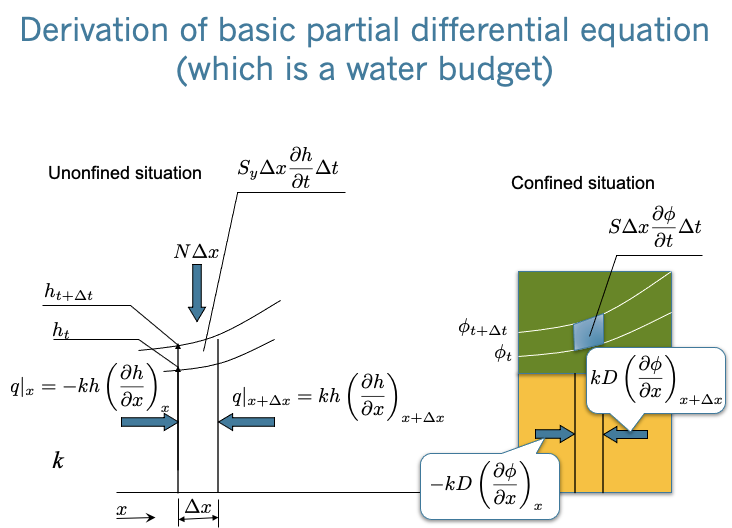
\includegraphics[width=0.8\textwidth]{pictures/water_budget_pde}
\par\end{centering}
\caption{\label{fig:Derivation-of-basic-1D-pde}Derivation of basic partial
differential equation (left an unconfined aquifer with $h$ the water-table
elevation and $S_{y}$ specific yield, and right a confined aquifer
with $\phi$ head, $S$ elastic storage coefficient)}
\end{figure}

We will treat analytical solutions for one layer only. Analytical
solutions for more than one layer exist and have been extended to
arbitrary numbers of layers in the 1980s by Kick Hemker and Kees Maas,
see for instance \textcite{HemkerC1985,Maas1986,HemkerC1987}. These
solutions require matrix computations, which were cumbersome at the
time, but which may nowadays be readily computed in programs like
Python. Nevertheless, we limit ourselves in this course to single-layer
cases.

Let us first derive the partial differential equation, starting with
continuity. Considering a small slice of an aquifer of length $\Delta x$
(cross section) and write its dynamic water budget in terms of flow
rates, assuming a constant aquifer thickness $D$

\[
\mbox{net in }=\mbox{rate into storage}
\]

\[
kD\left(\frac{\partial h}{\partial x}\right)_{x+\Delta x}-kD\left(\frac{\partial h}{\partial x}\right)_{x}+N\Delta x=S\Delta x\frac{\partial h}{\partial t}
\]

Dividing by $\Delta x$ and by $kD$ (assumed constant) yields

\[
\frac{\left(\frac{\partial h}{\partial x}\right)_{x+\Delta x}-\left(\frac{\partial h}{\partial x}\right)_{x}}{\Delta x}+\frac{N}{kD}x=\frac{S}{kD}\frac{\partial h}{\partial t}
\]

Letting $\Delta x\rightarrow dx$ yields

\[
\frac{\partial^{2}h}{\partial x^{2}}+\frac{N}{kD}=\frac{S}{kD}\frac{\partial h}{\partial t}
\]

We ignore the recharge $N$ in this course, as we can always superimpose
its effect so that with $N=0$ we get

\begin{equation}
\frac{\partial^{2}h}{\partial x^{2}}=\frac{S}{kD}\frac{\partial h}{\partial t}\label{eqcontinuit-equation-1D-1-1}
\end{equation}
Further notice that we may write $s\left(x,t\right)=h\left(x,t\right)-h_{0}$
where $s\left(x,t\right)$ is the head change relative to the initial
situation $h_{0}$, which may even depend on $x$.

Also notice that often $h$ is used for the head in a water table
aquifer, i.e. the elevation of the water table and $\phi$ for the
head in a confined or semi-confined aquifer, i.e. where there is not
water table. In fact, it matters little what symbol is used, as long
at its meaning is clearly stated.

This means that for 1D groundwater dynamics, we will mostly work with
solutions of the following partial differential equation where $s=s\left(x,t\right)$
is called the head change or often also the drawdown, especially when
dealing with groundwater extraction and wells

\begin{equation}
\frac{\partial s}{\partial t}=\frac{kD}{S}\frac{\partial^{2}s}{\partial x^{2}}\label{eq:diffusion-equation-in-s}
\end{equation}

Equation \ref{eq:diffusion-equation-in-s} is known as the diffusion
equation. It appears in many scientific fields like like diffusion,
dispersion, heat conduction, sorption, consolidation, etc. Many researchers
have derived solutions for this partial differential equation for
specific boundary and initial conditions. The coefficient $S/kD$
is called the diffusivity, often written as a thick D, like $\mathbb{D}$,
which always has dimension $\mathrm{\left[L^{2}/T\right]}$ whatever
the scientific application is. The diffusivity is the ratio of the
ease of the flow (transmissivity) and the storage:

\[
\mathbb{D}=\frac{kD}{S}
\]

In the case of a phreatic (unconfined, water-table) aquifer, the aquifer
thickness is no longer constant. Unfortunately, there are no transient
solutions that take a time-varying aquifer thickness into account.
Linearization is then unavoidable, meaning that one has to choose
a proper average aquifer thickness (or transmissivity) and remain
vigilant that the head change should remain small with respect to
the saturated thickness of the aquifer.

The partial differential equation can also be viewed in this basic
left-hand and right-hand parts

\[
kD\frac{\partial^{2}s}{\partial x^{2}}=S\frac{\partial s}{\partial t}
\]
in which the left-hand side describes the flow in the aquifer and
the right-hand side the storage. To readily understand and let sink
in the meaning of this partial differential equation, it is perhaps
easiest to integrate both sides over a distance $\Delta x$ to get

\[
kD\intop_{x}^{x+\Delta x}\frac{\partial^{2}s}{\partial x^{2}}dx=S\intop_{x}^{x+\Delta x}\frac{\partial s}{\partial t}dx
\]

which equals

\[
kD\left(\frac{\partial s}{\partial x}\rvert_{x+\Delta x}-\frac{\partial s}{\partial x}\rvert_{x}\right)=\left(S\Delta x\right)\frac{\partial s}{\partial t}
\]

This clearly shows that the left-hand side is the net inflow of a
piece with length $\Delta x$ (having dimension {[}L $^{2}$/T{]}
or {[}L $^{3}$/T{]} per unit length perpendicular to the cross section
of the aquifer, hence {[}L $^{2}$/T{]}, while the right-hand side
equals the storage over the same aquifer distance with $S$ {[}L $^{3}$/L
$^{2}$/L{]} (volume per unit of aquifer surface area per unit of
head increase per unit of time).

Also notice that

\[
\frac{\partial^{2}s}{\partial x^{2}}
\]
is the curvature of the head. Whenever that is positive, there is
an net inflow at the considered location originating from the aquifer
adjacent to the considered point or infinitesimally small section.

Finally notice that we can replace the head change $s$ (normally
used for (semi-)confined aquifers) by the absolute head $h$ (normally
used for water-table aquifers). This makes absolutely no difference
as only the derivatives of $s$ and $h$ play a role in the equation,
which are the same. Just read $s$ as head difference relative to
some initial or average condition.

\section{\label{sec:Sinusoidal-fluctuations}Sinusoidal fluctuations of the
groundwater head and flows}

This section deals exclusively with sinusoidal fluctuations of groundwater
heads and flows caused by a head of flow that fluctuates like a sine
at $x=0$. We deal with tidal fluctuations in groundwater first and
then show temperature as a second application of the same basic partial
differential equation.

\begin{figure}
\begin{centering}
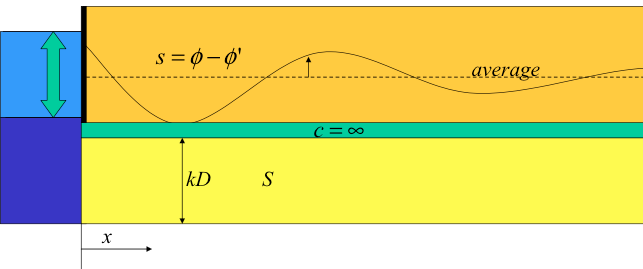
\includegraphics[width=0.8\textwidth]{pictures/tideSinusoidalFluctuation}
\par\end{centering}
\caption{\label{fig:Sinoidal-water-level-fluctuation}Sinusoidal water level
fluctuation in surface water causing tide in the groundwater system}
\end{figure}


\subsection{Groundwater fluctuations due to sinusoidal tides}

A number of transient problems can be analyzed by assuming sinusoidal
water-level or flow fluctuations at a boundary, at $x=0$ say. Generally,
the resulting heads and flows within the aquifer will then also behave
like a sine which will have the same frequency. If we have the analytic
solution for head or flow in the aquifer due to harmonic fluctuating
at the boundary, we may solve many related and more complex problems
by superposition, that is by combining solutions of arbitrary frequencies,
amplitudes and phase shifts. This way, hourly, daily, weekly and seasonal
fluctuations may be readily combined. Examples of applications are
tides in groundwater en the depth penetration of temperature fluctuations
at ground surface.

figure \ref{fig:Sinoidal-water-level-fluctuation} shows a cross section
through a confined aquifer (yellow) that extends to infinity at the
right. At $x=0$ this aquifer is in direct connection with a surface-water
body with a fluctuating water level, which causes fluctuations of
head and flow in the adjacent aquifer, which are delayed and dampened
relative to the forced fluctuation at $x=0$.

The partial differential equation for this system has already been
derived (see equation \ref{eq:diffusion-equation-in-s}). It may be
solved for a sinusoidal fluctuation of the water level at $x=0$.
We just assume the solution of the head $s$ in the aquifer relative
to the mean value without fluctuation, to be also sinusoidal with
the same frequency (same angular velocity $\omega$ {[}radians/T{]}),
but add a phase shift ( $-bx$) and assume an amplitude which is reduced
by the factor $e^{-ax}$ relative to the amplitude $A$ of the tide
at $x=0$:

\begin{equation}
s\left(x,t\right)=A\,e^{-ax}\sin\left(\omega t-bx\right)\label{eq:sine-solution-without-phase}
\end{equation}

The full tide time $T$ relates to the angular velocity $\omega$
as

\begin{equation}
\omega T=2\pi\label{eq:cycle-time}
\end{equation}

Notice that we can always change the phase of the tide by adding an
arbitrary angle $\nu$ to the argument of the sine. For an aquifer
with constant $kD$ and storage coefficient $S$ this solution is
indeed valid for

\begin{equation}
a=b\mbox{, so that }a=\sqrt{\frac{\omega}{2\mathbb{D}}}=\sqrt{\frac{\omega}{2}\frac{S}{kD}}\label{eq:aFluctuation}
\end{equation}

The proof is given in the box below. The proof fills the presumed
solution into the partial differential equation and sees under which
conditions the solution is true. It turns out to be as given in equation
\ref{eq:aFluctuation}. The relations may also be derived for the
situation in which the aquifer is semi-confined. Of course, this is
more complicated and beyond this course. However, the solution is
given in the box below for possible future reference.

\noindent{\fboxsep 6pt\fbox{\begin{minipage}[t]{1\columnwidth - 2\fboxsep - 2\fboxrule}%
\textbf{Semi-confined case (not for exam)}

Notice that in the semi-confined case, where linear tide-induced leakage
occurs between the aquifer and the overlying layer with constant head,
$a<>b$. In that was worked out in the PhD Thesis of Bosch (1951).
The results are

\begin{eqnarray*}
a & = & \frac{1}{\lambda}\sqrt{+\frac{1}{2}+\frac{1}{2}\sqrt{1-\left(\omega Sc\right)^{2}}}\\
b & = & \frac{1}{\lambda}\sqrt{-\frac{1}{2}+\frac{1}{2}\sqrt{1+\left(\omega Sc\right)^{2}}}\\
\lambda & = & \sqrt{kDc}
\end{eqnarray*}
%
\end{minipage}}}

Below the proof is given for the solution

\noindent{\fboxsep 6pt\fbox{\begin{minipage}[t]{1\columnwidth - 2\fboxsep - 2\fboxrule}%

\paragraph{Proof that the solution in equation\ref{eq:sFluctuaionStage} is
correct.}

We have to proof that equation \ref{eq:sine-solution-without-phase}
fulfills equation\ref{eq:diffusion-equation-in-s}. The constant is
dropped, as it does not affect the proof.

Taking the needed derivatives

\begin{eqnarray*}
\frac{1}{A}\frac{\partial s}{\partial x} & = & -a\,e^{-ax}\sin\left(\omega t-bx\right)-b\,e^{-ax}\cos\left(\omega t-bx\right)\\
\frac{1}{A}\frac{\partial^{2}s}{\partial x^{2}} & = & a^{2}\,e^{-ax}\sin\left(\omega t-bx\right)+ab\,e^{-ax}\cos\left(\omega t-bx\right)+\\
 &  & +ab\,e^{-ax}\cos\left(\omega t-bx\right)-b^{2}\,e^{-ax}\sin\left(\omega t-bx\right)\\
\frac{1}{A}\frac{\partial s}{\partial t} & = & \omega\,e^{-ax}\cos\left(\omega t-bx\right)
\end{eqnarray*}

by collecting the sines and the cosines separately, we get

\[
a^{2}-b^{2}=0\rightarrow a=b
\]

and so,

\[
2\frac{kD}{S}ab=2\frac{kD}{S}a^{2}=\omega\rightarrow a=\sqrt{\frac{\omega}{2}\frac{S}{kD}}
\]

Which completes the proof.%
\end{minipage}}}

As can be seen, an the arbitrary constant $\beta_{0}$ does not affect
the proof of correctness. This constant is merely a phase shift at
$t=0$. Therefore, the solution can also be given including this extra
phase shift at $t=0$, which may be useful when superimposing many
fluctuations that differ in amplitude was well as in phase:

\begin{equation}
s\left(x,t\right)=A\,e^{-ax}\sin\left(\omega t-ax+\beta_{0}\right)\label{eq:sFluctuaionStage}
\end{equation}

To see that $\beta_{0}$ is a phase shift, just fill in $x=0$ and
$t=0$.

The discharge is obtained by using Darcy

\begin{eqnarray}
Q\left(x,t)\right) & = & -kD\frac{\partial s}{\partial x}\nonumber \\
 & = & a\,kD\,A\,\left[e^{-ax}\sin\left(\omega t-ax+\beta{}_{0}\right)+e^{-ax}\cos\left(\omega t-ax+\beta{}_{0}\right)\right]\label{eq:QfluctuationStage}\\
 & = & a\,kD\,A\sqrt{2}\,e^{-\alpha x}\sin\left(\omega t-ax+\beta_{0}+\frac{\pi}{4}\right)
\end{eqnarray}

Hence, phase the flow is shifted by $\pi/4$ relative to the head.

As an example, figure  \ref{fig:sines_head_vs_x_and_vs_t} upper image
shows the head as a function of $x$ for different times and the lower
image shows the head as a function of $t$ at different distances
from the boundary. The upper figure   also shows the upper and lower
envelopes, although a bit difficult to see. The third picture is the
discharge as a function of time at different $x$-values. The head
in the second picture reaches its top when the discharge at the considered
point is already declining.

\begin{figure}
\begin{centering}
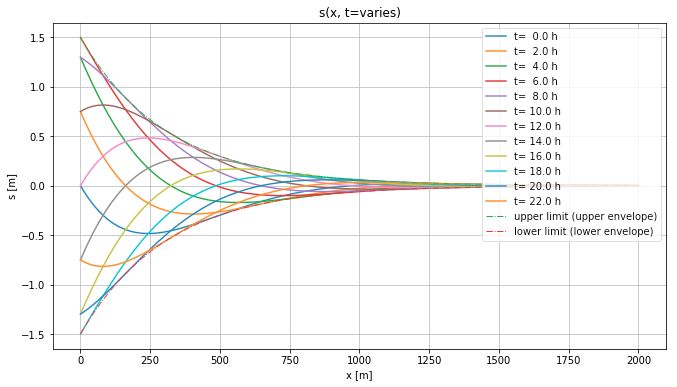
\includegraphics[width=0.75\textwidth]{pictures/sines_f_x}
\par\end{centering}
\begin{centering}
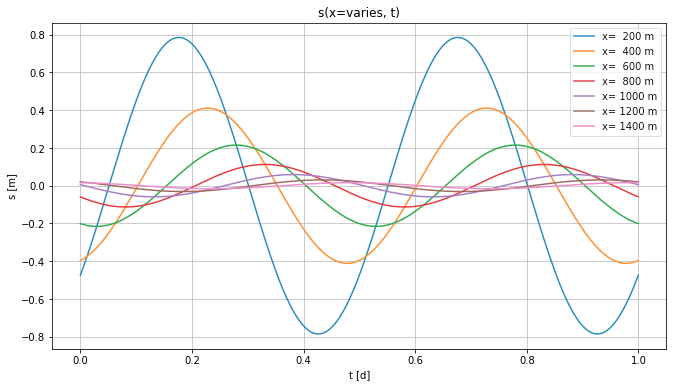
\includegraphics[width=0.65\textwidth]{pictures/sines_f_t}
\par\end{centering}
\begin{centering}
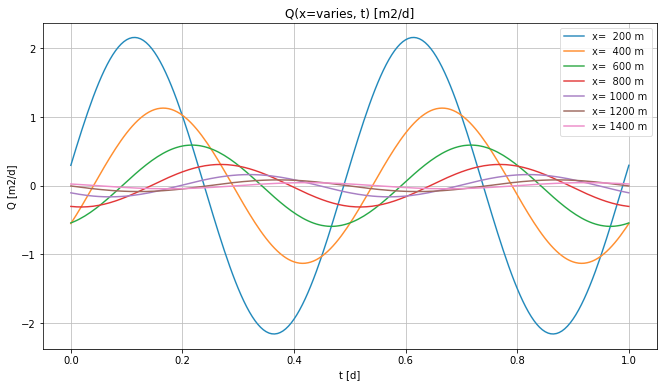
\includegraphics[width=0.65\textwidth]{pictures/sindes_Q_vs_t}
\par\end{centering}
\caption{\label{fig:sines_head_vs_x_and_vs_t}First picture: head as a function
of $x$ at different times, also showing the upper and lower envelopes.
Second picture: head as a function of t at different distances. $A=1.5$
m, $kD=600$ m$^{2}$/d, $S=0.001$, $\omega=4\pi$ (i.e. two full
tide cycles in 1~D). Third picture, discharge $Q$ {[}m$^{2}$/d{]}
(to the right positive) as a function of time for different $x$-values.}
\end{figure}


\paragraph*{\label{par:What-is-the-velocity}What is the velocity of the wave,
or what is the delay of the wave at any distance $x$ from the sea
or river?}

To find the answer, we move along with the wave such that the phase
is constant, e.a. equal to $c$. Hence

\[
\omega t-ax+\beta_{0}=c
\]

Then determine the velocity by computing $dx/dt$. So

\[
\omega-a\frac{dx}{dt}+0=0
\]

This leads to

\begin{equation}
v=\frac{dx}{dt}=\frac{\omega}{a}\label{eq:wave-velocity}
\end{equation}

The delay of the wave at any $x$ relative to the wave at $x=0$ is
then

\[
t=\frac{x}{v}
\]

The wave velocity can be measured in figure  \ref{fig:sines_head_vs_x_and_vs_t}
as the velocity of the top of the sines in the third figure .

Alternatively, one may say, that when the argument must be constant,
it doesn't matter which constant, but only constant, then we can just
well say that

\[
\omega t-ax=0
\]

so that immediately we have $x/t=\omega/a$, which is the same answer.

\paragraph*{How much is the wavelength in the ground?}

A direct approach is taking the argument of the sinus and demanding
that the argument of the sine at $t+T$ at $x$ (where $T$ is the
cycle time) is the same as the argument of the sine at $t$ but at
location $x+\Delta x$

\[
\left[\omega\left(t+T\right)-ax+\beta_{0}\right]=\left[\omega t-a\left(x+\Delta x\right)+\beta_{0}\right]
\]
hence

\[
\omega T=a\Delta x=0
\]

\begin{eqnarray*}
\Delta x & = & \frac{\omega}{a}T
\end{eqnarray*}
noting that the cycle time equals $T=\frac{2\pi}{\omega}$, we get

\[
\Delta x_{full\,wave}=\frac{2\pi}{a}
\]
with $a=\sqrt{\frac{\omega S}{2kD}}$, we also have

\[
\Delta x_{full\,wave}=2\pi\sqrt{\frac{2kD}{\omega S}}
\]

So, the larger $kD$ the longer the wave length, the larger the $S$
the shorter and the larger the $\omega$, the shorter the wavelength
will be, which all makes sense.

We have now seen that the head is indeed a damped sine. The damping
is stronger for higher frequencies, larger storage coefficients and
lower conductivities. It's difficult to measure the wave length from
the upper figure  in figure  \ref{fig:sines_head_vs_x_and_vs_t} because
the damping is so strong that essentially full damping takes place
within a single wavelength.

\subsection{Using characteristic time and length}

The solution may be more intuitively expressed using characteristic
time and length. The charactersitci time would be the cycle time,
$T$, i.e. it takes for one full tide to complete

\[
\omega T=2\pi\rightarrow T=\frac{2\pi}{\omega}\rightarrow\omega=\frac{2\pi}{T}\rightarrow\omega t=2\pi\frac{t}{T}
\]

Also, we could set a characteristic length of the tide the aquifer
to

\[
\lambda=\frac{1}{a}
\]

The envelopes are thus now expressed as

\[
-A\,e^{-\frac{x}{\lambda}}\le s_{x,t}\le+A\,e^{-\frac{x}{\lambda}}
\]
so that $\lambda$ now is the length over which the maximum amplitude
declines by a factor $e\approx2.3$.

The relation with the length over which the amplitude declines by
exactly a factor 2 is easily derived

\begin{align*}
e^{-\frac{x+\Delta x}{\lambda}} & =0.5e^{-\frac{x}{\lambda}}\\
-\frac{x+\Delta x}{\lambda} & =\ln0.5-\frac{x}{\lambda}\\
\Delta x & =\left(\ln2\right)\,\lambda\\
\Delta x & \approx0.69\,\lambda
\end{align*}

As always when we have an exponentially declining relationship, we
can define a half-time or half-length. That halftime or half-length
is always $\ln\left(2\right)\approx69\%$ of the characteristic time
of characteristic length, i.e. the time or length in which the exponent
declines by a factor $e\approx2.3$.

The characteristic length of the tidal wave in the aquifer is, therefore

\[
\lambda=\frac{1}{a}=\sqrt{\frac{2}{\omega}\frac{kD}{S}}=\sqrt{\frac{T}{\pi}\frac{kD}{S}}
\]
and the half-length is just 69\% of this.

Filling in the characteristic length and time gives

\[
h_{x,t}=A\,e^{-\frac{x}{\lambda}}\sin\left(2\pi\frac{t}{T}-\frac{x}{\lambda}+\theta\right)
\]

If one wishes to express all terms within the argument of the $\sin$
in terms of the full tidal cycle, one would write

\[
h_{x,t}=A\,e^{-\frac{x}{\lambda}}\sin\left(2\pi\left(\frac{t}{T}-\frac{x}{2\pi\lambda}+\frac{\theta}{2\pi}\right)\right)
\]

This directly shows that the distance $x=2\pi\lambda$ is the length
of a full wave in the subsurface, and, therefore, the expression $2\pi\lambda/T$
is the velocity of the wave in the subsurface.

\[
v=\frac{2\pi\lambda}{T}=\frac{2\pi}{T}\sqrt{\frac{T}{\pi}\frac{kD}{S}}=\sqrt{\frac{2\times2\pi}{T}\frac{kD}{S}}=\sqrt{\frac{2\times2\pi}{2\pi}\omega\frac{kD}{S}}=\sqrt{2\omega\frac{kD}{S}}
\]

\[
v=\frac{2\pi\lambda}{T}=\omega\sqrt{\frac{2}{\omega}\frac{kD}{S}}=\frac{\omega}{a}
\]

which is, what we already derived in paragraph \ref{par:What-is-the-velocity}
on page \pageref{par:What-is-the-velocity}. This all seems needlessly
complicated, but the take-home message is, that thinking in terms
of cycle time and characteristic length is easier for the human mind
and can be immediately translated to the field situation, while $\omega$
and the damping and delay factor $a$ really provide far little inspiration.

\subsection{Fluctuations of temperature in the subsurface}

For heat conduction in the subsurface, the same partial differential
equation (also called``diffusion equation'') applies if we replace
head change by temperature change. The only thing that changes is
the so-called diffusivity $kD/S$. The ease of flow, i.e. $kD$ with
groundwater flow, is now replaced by the heat conduction $\lambda\,\mathrm{\left[W/m\right]=\left[\left(\left(E/T\right)/L^{2}\right)/\left(K/L\right)\right]=\left[E/\left(TKL\right)\right]}$
and the storage is replaced by the heat capacity $\rho c\,\mathrm{\left[E/L^{3}/K\right]}$.
The dimension is again $\mathrm{\left[L^{2}/T\right]}$:

\[
\mathbb{D=}\frac{\lambda}{\rho c}\,\mathrm{\left[\frac{E/\left(TKL\right)}{E/\left(KL^{3}\right)}\right]=\left[\frac{L^{2}}{T}\right]}
\]
Notice that in the dimension $E$ = energy, $T$ = time, $L$ = length,
$K$ = temperature (from Kelvin). Because both the heat conduction
and the heat capacity consist of a contribution from both the water
and the grains (solids) of the aquifer, we can compute them as a porosity-weighted
combination of these contributions. With $\epsilon$ for porosity
we then have

\begin{eqnarray*}
\lambda & = & \epsilon\lambda_{w}+\left(1-\epsilon\right)\lambda_{s}\\
\rho c & = & \epsilon\rho_{w}c_{w}+\left(1-\epsilon\right)\rho_{s}c_{s}
\end{eqnarray*}
 $\rho\,\mathrm{\left[M/L^{3}\right]}$ is density and $c\,\mathrm{\left[E/\left(MK\right)\right]}$,
i.e. heat per kg solids per degree kelvin (= degree Celsius).

The heat capacity of saturated sandy soils is about $\lambda=3\,\mathrm{W/m/K}=3\,\mathrm{J/s/m/K}$.
The specific heat capacity of water is $c_{w}=4018\,\mathrm{J/kg/K}$
and that of sand grains $c_{s}\approx800\,\mathrm{J/kg/K}$. With
$\rho_{s}\approx2650\,\mathrm{kg/m^{3}}$ and $\epsilon\approx35\%$
we get $\rho c=2.85\times10^{6}\,\mathrm{J/m^{3}/K}$.

The diffusivity then becomes

\[
\mathbb{D}=\frac{\lambda}{\rho c}=\frac{3}{2.85\times10^{6}}=1.06\times10^{-6}\,\mathrm{m^{2}/s}=0.091\,\mathrm{m^{2}/d}
\]

From which we have

\[
a=\sqrt{\frac{\omega}{2\mathbb{D}}}=\sqrt{\frac{\pi}{T\mathbb{D}}}
\]

With these values, one can compute between what values the temperature
varies at any given depth as a function of the cycle time. For instance,
the temperature fluctuation due to daily, weekly, monthly or yearly
temperature fluctuations at ground surface. These envelopes are defined
by

\[
T_{mean}-A\,\exp\left(-az\right)\le temp\le T_{mean}+A\,\exp\left(-az\right)
\]
with $A$ {[}K{]} the temperature fluctuation amplitude at ground
surface.

The monthly temperature in the Netherlands varies between 3.1 $^{o}$C
in January and 17.9 $^{o}$C in July. The yearly amplitude is thus
7.4 $^{o}$C; the year mean temperature being 10.5 $^{o}$C. Using
this, we can compute the temperature envelopes, that is, the lowest
and highest temperatures between which the actual temperature will
vary. figure  \ref{fig:Temperature-envelopes-in-subsurface} shows
the results, as computed for the same mean temperature and the same
amplitude but for different cycle times as indicated in the legend.
With these data, the yearly temperature variation will barely reach
20 m below ground surface. Ten-year temperature fluctuations will
penetrate down to about 50 m and 30 year temperature variation would
be recordable down to about 100 m. This implies that climate change
may be measured using the change of the temperature at for instance
50 m below ground surface if measurements in the past are available,
as is actually the case in the Netherlands.

\begin{figure}
\begin{centering}
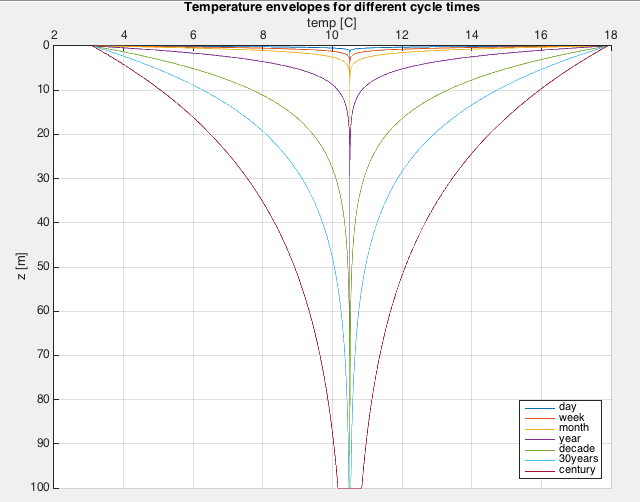
\includegraphics[width=0.6\textwidth]{pictures/temperatureEnvelopes}
\par\end{centering}
\caption{\label{fig:Temperature-envelopes-in-subsurface}Temperature envelopes
in the subsurface due to temperature fluctuations at ground surface
with mean 10 $^{o}$C and amplitude 7.4 $^{o}$C. Envelopes depend
on cycle time of the fluctuation (see legend).}
\end{figure}


\subsection{Concluding remarks}

The derived partial differential equation applies to both groundwater
flow and heat conduction. The only change is that head change is replaced
by temperature change, transmissivity by heat conductance and the
storage coefficient is replaced by heat capacity. Both heat conductance
and heat capacity can be computed as a porosity weighted average of
the contribution of the water and of the grains.

Sinusoidal analysis is useful to study the impact of ongoing fluctuations
of the input on the groundwater. It is straightforward to compute
the head and temperature envelopes defining the limits of a given
sine input at a given distance or depth. Often, this is enough he
understand the physics and estimate potential impact. Most importantly
it is enough the understand the relation between the different parameters
that play in this setting.

More complicated inputs can be constructed as a sum of a number of
sin (or cosine) fluctuations, each with its own amplitude, frequency
and phase shift. In fact, any input can be so constructed, although
this may require the summation of many waves. On the other hand a
given i.e. measured input may be split into individual waves using
Fourier Analysis. Python has modules for that. This helps to find
the dominant ones, and allows limiting the following analysis on only
a few dominant waves. This simply means that this sinusoidal solution
of the partial differential equations offers many ways to analyze
groundwater systems of the type we considered. By superposition, these
analysis can also be combined with other features such as wells.

\subsection{\label{subsec:Questions-5-3-5}Questions}
\begin{enumerate}
\item Prove the correctness of the given solution yourself. As an extra
exercise you could prove that equation \ref{eq:QfluctuationStage}
is correct by filling it into the partial differential equation for
continuity $\frac{\partial Q}{\partial x}=-kD\frac{\partial^{2}s}{\partial x^{2}}=-S\frac{\partial s}{\partial t}$.
\item If the transmissivity is doubled, what is the effect on the drawdown?
\item When the $\omega$ is doubled, what is the effect on the drawdown?
\item Explain how the distance to where the fluctuation of the sea or lake
reaches in the aquifer depends on the frequency of the wave.
\item How far in-land reaches the effect of waves on the beach with one
cycle per second, tides with one cycle per 12 hours, moon-tides with
one cycle per two weeks in an aquifer with transmissivity is $kD=500$
m$^{2}$/d and a storage coefficient of $S=0.001$ and $S=0.1$ respectively?
\item Let the solution to the diffusion equation for the confined aquifer
be $s\left(x,t\right)=A\,\exp\left(-ax\right)\sin\left(\theta_{0}+\omega t-ax\right)$
and let $kD=1000\,\mathrm{m^{2}/d},$ $S=10^{-3}$, and the amplitude
$A=2\,\mathrm{m},$ and let $\theta_{0}$ be an arbitrary constant.
Take time in days and show the head change $s\left(x,t\right)$ in
Python or in Excel. With this, answer the following 5 sub-questions:
\item Include the discharge $Q\left(x,t\right)$
\item Compute and also show the envelope of the wave as a function of $x$.
\item How far inland can we still measure the tide if our device allows
us to see a variation of 1 cm?
\item What is the velocity of the wave?
\item What is the delay at 1000 m from the shore (or show the delay graphically
as function of $x$)?
\item Add the case for a storage coefficient, $S_{y}=0.2$. And show the
relation between the case with $S=0.001$ and $S_{y}=0.2$.
\item Create a complex input using of 4 sines, each with a different initial
angle $\theta_{0}$, amplitude $A$ and angular velocity $\omega$
and show the result.
\end{enumerate}
Copy your code and alter the copy to answer the following questions:
\begin{enumerate}
\item The head in a lake above a clay bottom varies daily 30 cm. How deep
does this fluctuation penetrate the underlying clay layer with conductivity
of $10^{-4}$ m/d and a specific storage coefficient of $S_{s}=0.0001$
/m? Assume that you could still measure variations down to 3 mm.
\item What if the variation is weekly, monthly and seasonally only?
\item If the sea is shallow and the clay layer is below the sea bottom,
what will be the amplitude in the confined aquifer for the water compressibility
$\beta_{w}=5\times10^{-5}$ and porous matrix compressibility $\beta_{s}=2\times10^{-5}\,\mathrm{m^{2}}/N$?
\item If the clay layer would be semi-pervious, what would this mean for
the amplitude in the confined aquifer? Would it be greater, smaller
compared with the case with a completely impervious layer?
\end{enumerate}

\paragraph*{Heat flow}
\begin{enumerate}
\item What is the penetration depth of a diurnal (twice-a-day), seasonal
and centennial temperature fluctuation at ground surface given $\lambda=3$~W/m/K,
$\rho_{s}c_{s}=0.800$~MJ/m $^{3}$/K and $\rho_{w}c_{w}=4.2$~MJ/m
$^{3}$/K and porosity of $\epsilon=0.35$?
\item Heat flow and groundwater flow show the same partial differential
equation except that head change is replaced by temperature change.
They both have one coefficient called diffusivity. What is the dimension
of this diffusivity in both situations?
\item Diffusivity consists of a part that expresses the ease of flow, $\lambda$,
and a part that expresses the storage, $\rho c$. What are the equivalent
factors in the groundwater case?
\item Groundwater flow was ignored when we discussed heat flow. Describe
how temperature envelopes would change due to upward groundwater seepage,
would they shrink or stretch?
\item How would these envelopes change due to downward seepage? How much
would you estimate the effect on the yearly temperature envelopes
if the recharge is 333 mm per year and porosity is 33\%? First estimate
how deep the recharge penetrates in one year.
\end{enumerate}

\section{Non-fluctuating interaction with surface water}

In the previous section, we discussed the effect of sinusoidal variation
of the level of a surface water that is in direct contact with a confined
or unconfined aquifer. In this chapter, we'll discuss the same hydrological
setting, but in which the surface water level changes suddenly by
a fixed amount.

\subsection{\label{subsec:Basins-of-half-infinite-lateral-extent}Basins of half-infinite
lateral extent}

Again, we consider a confined aquifer in direct contact with surface
water as was done in the previous section. The situation is depicted
in figure  \ref{fig:One-dimensional-groundwater-basin-rise-a}. The
aquifer thickness, transmissivity and storage coefficient are everywhere
the same. The aquifer is half-infinite, which means that its right
end extends to infinity. We consider the aquifer as confined, because
we will assume that its thickness is the same everywhere and stays
so. This is required only to allow a closed analytical solution for
the time-dependent groundwater flow. There are no time-dependent closed
analytical solutions for water-table aquifers in which the transmissivity
varies along with the head and, therefore, with time. We further assume
the aquifer being in direct contact with the surface water. This implies
that there is no hydraulic resistance of any kind between the surface
water and the aquifer. This assumption keeps the analysis simple.
However, solutions exist that take hydraulic resistance between the
surface water and the aquifer into account as outlined in \textcite{Bruggeman1999},
but are beyond this course.

We present here a basic analytical solution, which describes the change
of head (and flow) caused by a sudden change of the surface-water
level by an amount $A$ {[}m{]}.

In the confined case we use the elastic storage coefficient, $S=DS_{s}$
and in the unconfined case we use the specific yield, $S_{y}$. In
cases where we consider unconfined aquifers, the effective thickness
of the aquifer changes along with the water table, and, therefore,
also with the head. However, as long as the change of head is small
compared to the thickness of the aquifer, we may still apply the solution
in practice and accept the small error caused by the assumption of
constant thickness.

Initially, the head is $\phi'$ in figure  \ref{fig:One-dimensional-groundwater-basin-rise-a}
and the head $\phi\left(x,t\right)$ varies in space and time due
to a sudden change of head of the bounding surface water by an amount
of $A$ m at $t=0$. The surface-water head remains at $\phi'+A$
thereafter.

Because superposition applies (due to linear governing partial differential
equation), we may just superimpose the change of head $s\left(x,t\right)=\phi\left(x,t\right)-\phi'$,
irrespective of the actual situation. The only thing that matters
to us. is the\textbf{ change of head} $s$ that is caused by the sudden
change of the water level in the bounding surface water by $A$ m.

The case considered here is a base case. There exists a series of
analytical solutions for other boundary conditions, which is presented
in section \ref{sec:Higher-level-solutions}. These solution are given
for reference only, not for the exam.

\begin{figure}
\begin{centering}
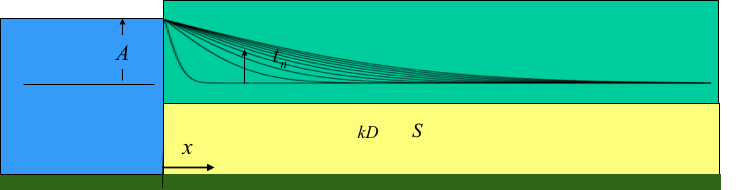
\includegraphics[width=0.8\textwidth]{pictures/StripWaterLevelOneSideBya}
\par\end{centering}
\caption{\label{fig:One-dimensional-groundwater-basin-rise-a}One-dimensional
groundwater aquifer which extends to infinity to the right, and has
constant transmissivity $kD$ and storage coefficient $S$, while
it is in direct contact with surface water at $x=0$ in which the
water level is suddenly changed by $a$ at $t=0$}
\end{figure}

Consider a one-dimensional aquifer of infinity lateral extent as shown
in figure  \ref{fig:One-dimensional-groundwater-basin-rise-a} that
is in direct contact with a fully penetrating water body at $x=0$.
Ignoring leakage and recharge, and assuming a constant transmissivity
$kD$ and storage coefficient $S$, the partial differential equation
is the diffusion equation:

\begin{equation}
kD\frac{\partial^{2}s}{\partial x^{2}}=S\frac{\partial s}{\partial t}\label{eq:diffusion-equation}
\end{equation}

The most well-known solution of this series of solutions is the one
in which the head at $x=0$ is suddenly raised at $t=0$ by a $A$
m, and then further maintained (figure  23).

This solution is

\[
s\left(x,t\right)=\phi\left(x,t\right)-\phi_{0}=A\,\mathrm{\mbox{erfc}}\left(u\right)\mbox{, with }u=\sqrt{\frac{x^{2}S}{4kDt}}
\]
Where $s\left(x,t\right)$ is the head change, $\phi\left(x,t\right)$
the head and $\phi_{0}\left(x\right)$ the initial head that may be
any function if $x$, because it does not interfere with the principle
of superposition.

By definition

\begin{equation}
\mbox{erfc}\left(z\right)=\frac{2}{\sqrt{\pi}}\intop_{z}^{\infty}e^{-y^{2}}dy\label{eq:erfc-solution}
\end{equation}
and so its derivative is

\[
\frac{d\,\mathrm{erfc}\left(z\right)}{dz}=-\frac{2}{\sqrt{\pi}}e^{-z^{2}}
\]
Therefore, the discharge is

\[
Q=-kD\frac{\partial s}{\partial x}=A\,\sqrt{\frac{kDS}{\pi t}}\exp\left(-\frac{x^{2}S}{4kDt}\right)
\]
and, for $x=0$

\[
Q_{0}=A\,\sqrt{\frac{kDS}{\pi t}}
\]

The function $\mbox{erfc}(-)$ is the so-called complementary error
function.

\textcite{Abramowitz1972} provide tables and expressions to compute
this function in several ways. The erfc function is available in Excel
as well as in Python. Its graph is shown in figure  \ref{fig:Erfc(u)}

\begin{figure}
\begin{centering}
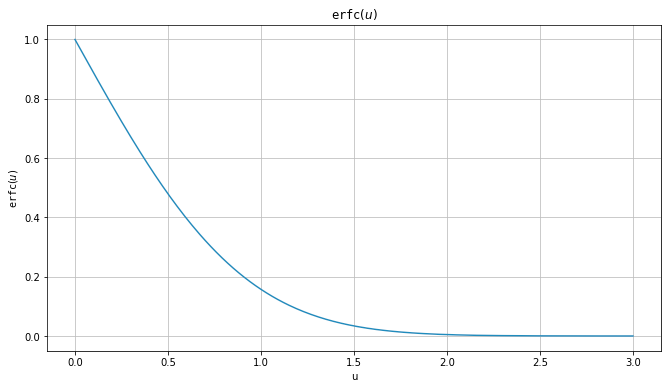
\includegraphics[width=0.8\textwidth]{pictures/erfcFunction}
\par\end{centering}
\begin{centering}
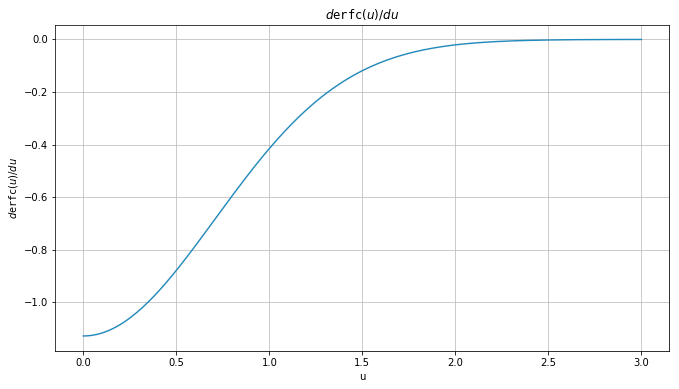
\includegraphics[width=0.8\textwidth]{pictures/erfcFunction_derivative_off}
\par\end{centering}
\caption{\label{fig:Erfc(u)} $\mbox{erfc}(u)$ and its derivative $-\left(2/\sqrt{\pi}\right)\exp\left(-u^{2}\right)$}
\end{figure}

Hence, the solution of the head change versus distance to the shore
always has the shape of this curve, be it that the horizontal axis
will be squeezed or stretched depending on the values of the parameters
in $u$. The shorter the time, the larger $u$, the more compressed
is the horizontal axis. A small $kD$ or large $S$ also has the effect
of compressing the horizontal axis.

For the understanding it is convenient to express $u=x/L$ so that
$L=\sqrt{4kDt/S}$, which is a constant for any fixed $t$. For this
fixed $t$, $L$ may be considered a characteristic distance, as it
scales $x$. For instance, half of the initial head change has been
reached when $u\approx0.5$ that is at a distance $x=0.5L$. Also,
the head change is about 10\% of $A$ at $u=1$, that is at $x=L$,
with $L$ fixed for the time of observation. No head rise has yet
occurred for about $u=2.5$, hence, for $x>2.5L$. This is all practical
information when judging an actual situation, without the need for
a computer.

The solution is only valid for $u>0$, this is clear for $x^{2}$
under the square root and $t>0$. But when we express $u$ as $u=x\sqrt{\frac{S}{4kDt}},$this
is not so obvious. However $x$ is must be positive and seen as the
distance from the point of consideration to the boundary with the
head change. So in case this boundary as a coordinate $x_{b}$ and
our point of consideration is $x_{0}$ we should use $x=\left|x_{0}-x_{b}\right|$
in the formula of $u$, hence, treat $x$ as a distance, being always
positive.

It is also possible to plot $\mbox{erfc}\,u$ and its derivative versus
$1/u^{2}$. To make the graph meaningful, we have to use a logarithmic
scale for $1/u^{2}$ as is shown in figure  \ref{fig:erfcand-its-derivative-versus-1overu}.
The time scale is then proportional to $t$. We can write $u^{2}=T/t$
with $T=x^{2}S/\left(4kD\right)$, where $T$ can be considered a
characteristic time for fixed distance $x$. We see that for $t/T\approx2$,
about half the final (maximum) head change has been reached. It is
useful and practical to consider this graph from the perspective of
$t/T$ instead of just $t$. Taking this perspective, one only needs
a single graph to cover all possible cases; the only thing that changes
when choosing another observation point is the value of the characteristic
time $T$. Then $T$ can be considered time characteristic for the
situation at a chosen distance $x$. The graph in figure  \ref{fig:erfcand-its-derivative-versus-1overu}
also shows that some time elapses before the influence of the river
reaches the observation point. The value of $1/u$ for this time is
about 0.4 as can be read from figure  \ref{fig:erfcand-its-derivative-versus-1overu}.
Hence, $t/T=0.16$. This result is also universal. 90\% of the final
head is reached at about $1/u^{2}=100$, so that $t=100T$.

For the discharge, we need the derivative, which is also shown in
both figures.

\begin{figure}
\begin{centering}
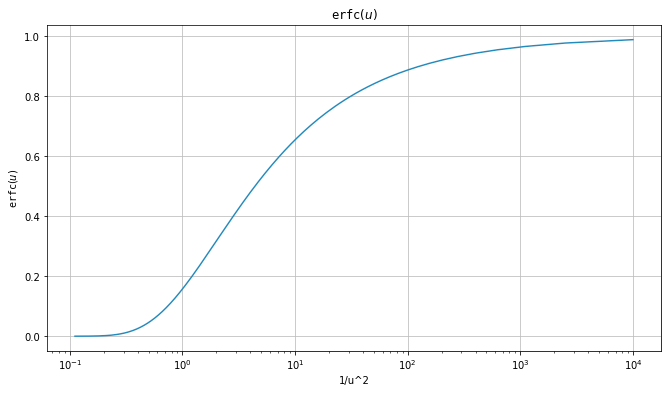
\includegraphics[width=0.8\textwidth]{pictures/erfcFunction_vs_u-2}
\par\end{centering}
\begin{centering}
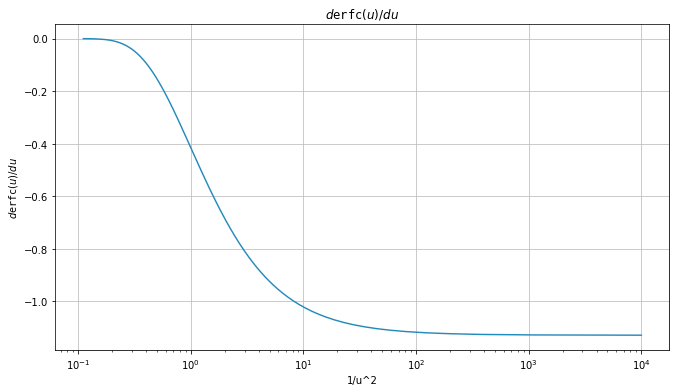
\includegraphics[width=0.8\textwidth]{pictures/erfcFunctionAndDerivative_vs_u-2}
\par\end{centering}
\caption{\label{fig:erfcand-its-derivative-versus-1overu}erfc$\left(u\right)$and
its derivative as a function of $1/u^{2}$ instead of vs. $u$. This
makes the horizontal axis proportional to time, as $1/u^{2}=\frac{4kD}{x^{2}S}t$.}
\end{figure}


\paragraph{Exercise:}

Proof that equation \ref{eq:erfc-solution} fulfills the partial differential
equation \ref{eq:diffusion-equation}.

\subsection{\label{subsec:Questions-5-4-2}Questions}
\begin{enumerate}
\item All drawdowns due to a sudden change of river stage are expressed
in a simple erfc-function. Can you express the argument $u$ using
a ratio of the distance $x$ from the river and some characteristic
distance $X$ that is valid for a fixed time?
\item What is the ratio $x/X$ for $s\left(x\right)=0.5s_{0}$, i.e. $s$
is half the head change at $x=0$?
\item Alternatively, how could you express the head change as a ratio of
time $t$ and a characteristic time $T$ for a fixed distance?
\item What is then the ratio $t/T$ for $s=0.5s_{0}$?
\item At what time, expressed at $t/T$, would you expect the head in the
aquifer to start changing at some given fixed distance $x$ after
a sudden change of river stage at $x=0$?
\item Given the mathematical expression for the head change, derive the
expression for the discharge $Q\left(x,t\right)$.
\item What is the discharge at $x=0$ mathematically?
\item An aquifer with properties $kD=400\,\mathrm{m^{2}/d},\,S=0.1$ is
in good contact with a river. The water level in the river rises by
2 m in a vary short time. What is the effect of this change for a
points $x$ at 10, 100 and 1000 m?
\item How long does it take for the head change in the three points to reach
10 cm?
\item Using Python, show the head over time in these points.
\item Using Python, show the discharge over time in these points.
\item How long will it take until the head in the center of a 10 m thick
aquitard with resistance $c=5000$ d and a specific storage coefficient
$S_{s}=10^{-5}$ m $^{-1}$ has reached half the head change that
was suddenly applied at both its top and bottom at $t=0$?
\end{enumerate}
A canal in a dune area is used to provide storage for drinking water
in the case of an emergency. The aquifer properties are $kD=100\,\mathrm{m^{2}/d}$,
$S=0.2$. During such an emergency, the water level in the 50 m wide
canal is suddenly lowered by 5 m.
\begin{enumerate}
\item How much water will flow into the storage canal from two sides in
1 day, 1 week, 6 weeks?
\item Compare these amounts with the amount of water stored in the canal?
\item What will be the drawdown over time at 10, 100, 300, 1000m?
\item Compute the flow to the canal in 6 weeks if there is a fixed-head
boundary at 70 m distance. You must use superposition to compute this.
\end{enumerate}

\subsection{\label{sec:Higher-level-solutions}Higher-order solutions (not for
exam)}

The previous well-known basic solution is the first of an infinite
series of solutions of the same partial differential equation but
for different boundary conditions, namely $s\left(0,t\right)=a\,t^{n/2}$
with $a$ a constant and $n\ge0$. The solution given above is for
$n=0$.

The entire series of solutions is given is given in \textcite{Carslaw1986}
and \textcite{Bruggeman1999} but can be more conveniently written
as

\[
s\left(x,t\right)=A\,t^{n/2}\frac{\mbox{i}^{n}\mbox{erfc}\,u}{\mbox{i}^{n}\mbox{erfc}\,0}\mbox{, with }u=\sqrt{\frac{x^{2}S}{4kDt}}
\]
The function $\mbox{i}^{n}\mbox{erfc}\,u$ is the $n^{th}$ repeated
integral of the complementary error function (Section 7.2 in \textcite{Abramowitz1972}).
A number of these functions is shown in figure  \ref{fig:-higher-order-erfc-functions}.
These higher order repeated integrals are not in Abramowitz and Stegun
(1964) but can be easily computed using a recursive expression given
below.

By definition

\[
\mbox{i}^{n}\mbox{erfc}\,z=\intop_{z}^{\infty}\mbox{i}^{n-1}\mbox{erfc}\left(\zeta\right)d\zeta
\]
 with

\[
\mbox{i}^{0}\mbox{erfc}\,z=\mbox{erfc}\,z
\]
and

\[
\mbox{i}^{-1}\mbox{erfc}\,z=\frac{2}{\sqrt{\pi}}e^{-z^{2}}
\]

Higher order functions may be computed by the following recursive
relation

\[
\mbox{i}^{n}\mbox{erfc}\,z=\frac{-z}{n}\mbox{i}^{n-1}\mbox{erfc}\,z+\frac{1}{2n}\mbox{i}^{n-1}\mbox{erfc}\,z
\]

By applying Darcy's law, we find the discharge

\[
Q\left(x,t\right)=\frac{\sqrt{kDS}}{2\sqrt{t}}A\,t^{n/2}\frac{\mbox{i}^{n-1}\mbox{erfc}\,u}{\mbox{i}^{n}\mbox{erfc}\,0}
\]

Instead of expressing $s\left(0,t\right)=At^{n/2}$ we could write
$Q\left(0,t\right)=Bt^{n/2}$, $n\ge0$. This is more convenient when
we like to specify the flow instead of the head. If we just write
$\frac{\sqrt{kDS}}{2\sqrt{t}}A=B$, we get

\[
Q\left(x,t\right)=B\,t^{n/2}\frac{\mathrm{i^{n-1}erfc}\,u}{\mathrm{i^{n}erfc}\,0}
\]

and at the same time

\[
s\left(x,t\right)=\frac{2\sqrt{t}}{\sqrt{kDS}}B\,t^{n/2}\frac{\mathrm{i^{n}erfc}\,u}{\mathrm{i^{n}erfc}\,0}
\]

A basic solution is obtained by setting $n=0$, so that $Q\left(0,t\right)=B$
is constant. In that case, the head at $x=0$ declines according to
the $\sqrt{t}$. When the discharge increases linearly, the head at
$x=0$ changes according to $t\sqrt{t}$. On the other hand, when
the drawdown is constant at $x=0,$ the discharge is inversely proportional
to $\sqrt{t}$ and when the head at $x=0$ rises linearly with time,
the discharge increases according to $\sqrt{t}$.

These functions may be used to compute the head and flow due to either
a constant or changing head at $x=0$ or due to a constant or changing
flow at $x=0$. Computations are easily done in Python or even in
Excel after the functions have been implemented.

\begin{figure}
\begin{centering}
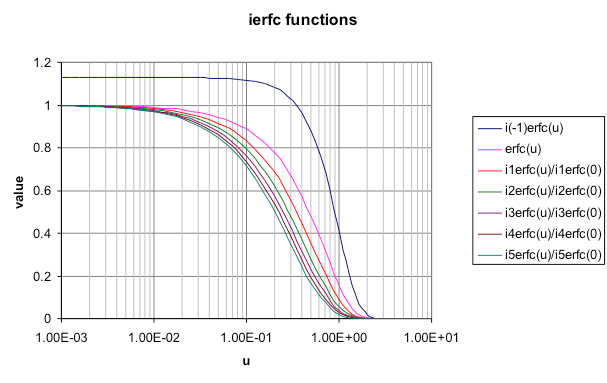
\includegraphics[width=0.8\textwidth]{pictures/ierfcFunctions}
\par\end{centering}
\caption{\label{fig:-higher-order-erfc-functions} $\mbox{i}^{n}\mbox{erfc}$
functions}
\end{figure}


\paragraph{Example:}

For instance, the water level in Lake Nasser in Egypt has risen by
60 m between the mid 1960s, when the dam at Aswan was closed, and
the end of the 1980s, when the new lake was full. This boils down
to rise of the lake level of about 3 m/year. Just assume that the
bordering aquifer is 200 m thick and that it has a conductivity $k=1\,\mathrm{m/d}$
and a specific yield $S_{y}=0.1$. How far would the effect of the
filling of the lake reach in the adjacent aquifer? How much lake water
would have been stored in that aquifer in that same period?

Using the expression and setting $n=2$ and $A=3$ m/y, we have

\[
s\left(x,t\right)=A\,t^{n/2}\frac{\mbox{i}^{n}\mbox{erfc}\,u}{\mbox{i}^{n}\mbox{erfc}\,0}\mbox{, with }u=\sqrt{\frac{x^{2}S}{4kDt}}\mbox{ and with }A=3\,\mathrm{m/y}\mbox{ and further }n=2
\]
This specifies a linear rise of the lake level over time. With $n=2$
we get

\[
s\left(x,t\right)=A\,t\frac{\mbox{i}^{2}\mbox{erfc}\,u}{\mbox{i}^{2}\mbox{erfc}\,0}\mbox{, with }Q\left(x,t\right)=\sqrt{\frac{kDS}{4t}}A\,\frac{\mbox{i}^{1}\mbox{erfc}\,u}{\mbox{i}^{2}\mbox{erfc}\,0}
\]

With proper values of $kD$ and $S$, a graph can be made for $s$
and $Q$ as a function of $x$ for given times. Alternatively, we
can make graphs of $s$ and $Q$ as a function of time for given values
of $x$. The results are shown in figure  \ref{fig:Lake-Nasser-example.}.
The top figure  shows the head in the aquifer as a function of $x$
for different times. The middle figure  shows the infiltration at
$x=0$ as a function of time. The bottom figure  shows the development
of the head over time at different distances from the lake bank. Note
that the lake level remains constant after $t=20$ years. The head
at $x=0$, therefore, remains equal till the lake level reaches a
total rise of 60 m thereafter. After that, the lake level is kept
constant. The infiltration $Q$ then sharply declines because the
head does not rise further. This reaching of a constant lake level
is implemented by superimposing the solution for a lake with a water
level that declines with the same speed (i.e $A=-3$ m/y) starting
at the moment the top lake-level is reached. It is a good exercise
to implement this yourself.

Of course, the same case can be simulated using the function for a
sudden rise of the lake level. But then the actual gradual rise of
the lake level must be subdivided into many small sudden steps, the
result of which must be added together (i.e. superimposed) to obtain
the overall solution. The results is shown in figure  \ref{fig:Lake-Nasser-example_sudden_changes}.
The rise of the head and lake are shown in the lower picture, the
flow at $x=0$ is shown in the picture in the middle. The results
are essentially the same, but the infiltration at $x=0$ fluctuates
quite heavily under the discrete yearly sudden head increments of
3 m each. At larger distances, however, these steps damp out. Of course,
the smaller the steps, the smoother the result will be. This example
shows that it may be much more convenient and require less work to
directly apply the solution for the linear rise of the head at $x=0$.

\begin{figure}
\begin{centering}
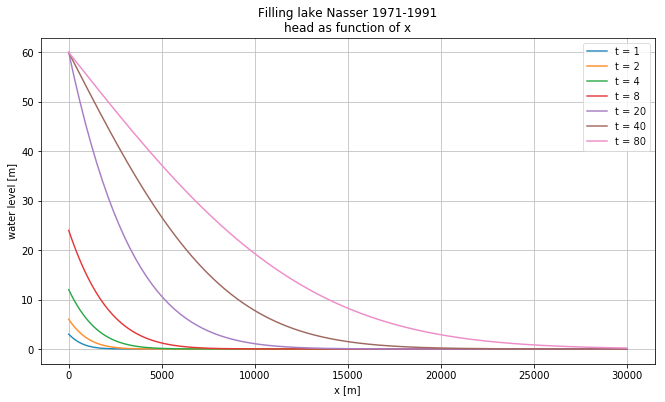
\includegraphics[width=0.7\textwidth]{pictures/lakeNasserLevel}
\par\end{centering}
\begin{centering}
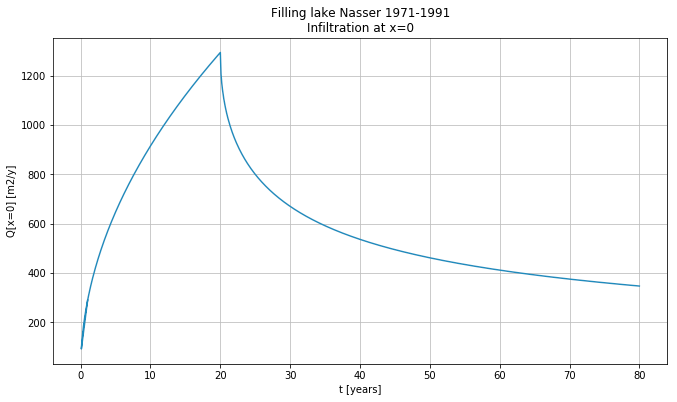
\includegraphics[width=0.7\textwidth]{pictures/lakeNasserInf_at_x0}
\par\end{centering}
\begin{centering}
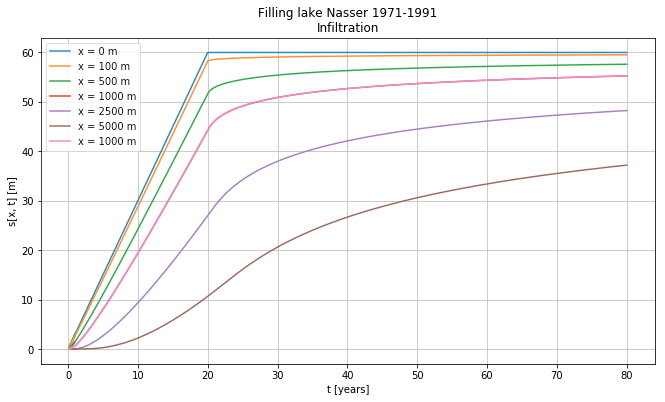
\includegraphics[width=0.7\textwidth]{pictures/lakeNasserLevel_for_xs}
\par\end{centering}
\caption{\label{fig:Lake-Nasser-example.}Lake Nasser example. Top: the head
in the adjacent aquifer as a function of $x$, the distance to the
shore, at different times. Middle: The infiltration into the aquifer
at $x=0$ as a function of time. Bottom: The head development over
time at different values of $x$}
\end{figure}

\begin{figure}
\begin{centering}
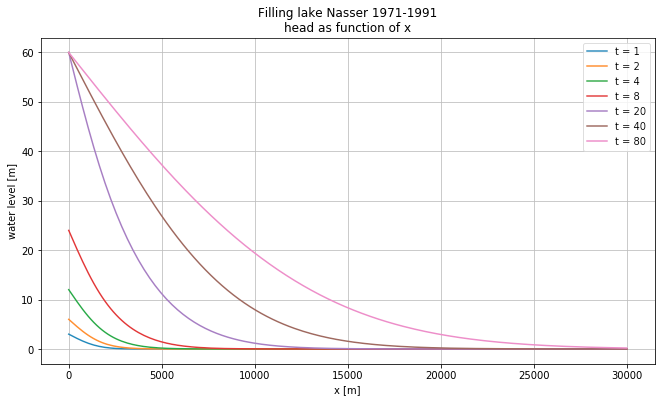
\includegraphics[width=0.7\textwidth]{pictures/lakeNasserLevel_sudden}
\par\end{centering}
\begin{centering}
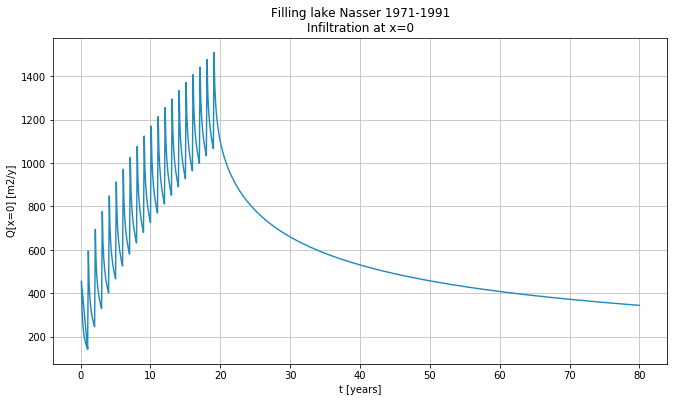
\includegraphics[width=0.7\textwidth]{pictures/lakeNasserInf_at_x0_sudden}
\par\end{centering}
\begin{centering}
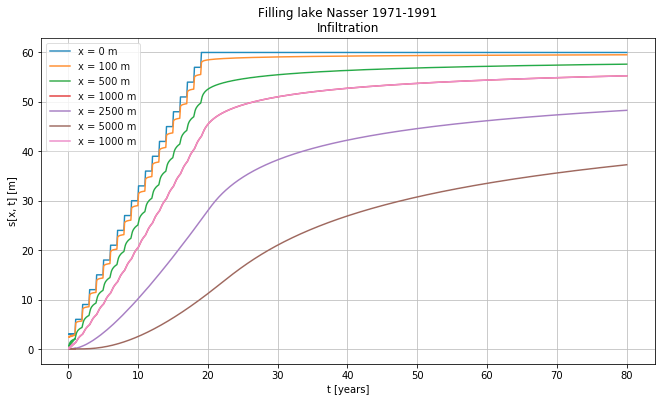
\includegraphics[width=0.7\textwidth]{pictures/lakeNasserLevel_for_xs_sudden}
\par\end{centering}
\caption{\label{fig:Lake-Nasser-example_sudden_changes}Lake Nasser example,
simulated using the solution for a sudden change and dividing the
linear rise over 20 years in 20 sudden changes of equal size. Top:
the head in the adjacent aquifer as a function of $x$, the distance
to the shore, at different times. Middle: The infiltration into the
aquifer at $x=0$ as a function of time. Bottom: The head development
over time at different values of $x$}
\end{figure}


\subsection{\label{subsec:Questions-5-4-4}Questions}
\begin{enumerate}
\item What is the mathematical expression for the head $s\left(x,t\right)$
and the discharge $Q\left(x,t\right)$ for the case in which the river
stage increases linearly with time?
\item What is the mathematical expression for the case in which the discharge
increases linearly with time.
\item Let a lake (like Lake Nasser) have a water level that rose linearly
by 60 m between 1971 and 1991. Compute the change of head in the aquifer
at 1 km from to the lake. Assume the $kD=1000\,\mathrm{m^{2}/d}$
and $S=0.1$.
\item Compute the total amount of water that infiltrated over this period.
\item Assume the aquifer has a constant thickness and its porosity is 35\%.
With this information compute how far the lake water penetrated the
aquifer during this period.
\item When, after 1991, the water level has been more or less constant,
then how much is the infiltration $Q\left(0,t\right)$ at the lake
shore in 2021? By how much has it declined since 1991?
\end{enumerate}

\subsection{\label{subsec:Superposition-in-time-half-inf-aquifer}Superposition
in time, half-infinite aquifer}

Consider a half-infinite aquifer in direct connection with surface
water at $x=0$. The analytical solution for the change of the groundwater
head $s\left(x,t\right)$ that is caused by a sudden change of the
surface water level by an amount $A$ at $t=0$, which was given before
:

\[
s\left(x,t\right)=A\,\mathrm{erfc}\sqrt{\frac{x^{2}S}{4kDt}}\mbox{, with }t\ge0\mbox{, where }s\left(x,t\right)=0\mbox{ for }t<0
\]

The head change $s\left(x,t\right)$ due to an arbitrary sudden change
of the surface-water level by an amount $A_{i}$ happening at $t_{i}$
can be obtained by superposition as usual. Using $i$ as an event
index, we then get

\[
s\left(x,t\right)=\sum_{i=1}^{N}\left\{ dA_{i}\,\mathrm{erfc}\sqrt{\frac{x^{2}S}{4kD\left(t-t_{ci}\right)}}\right\} \mbox{, with }t\ge t_{i}
\]

Each term is nonexistent, hence zero, for $t<t_{i}$. The surface-water
level at any time is $s\left(0,t\right)=\sum_{1}^{N}dA_{i}\mbox{, with }t>t_{ci}$,
because each sudden change of water level is supposed to last forever
after it happened at $t_{ci}$. This way, one can compute the head
change and, of course, the flow in an aquifer due to an arbitrary
variation of the surface water level at $x=0$. Of course, if the
surface water would vary continuously, like one or more $sine$ functions,
one would rather use the solution for a sine boundary head to simplify
the computations. Even a combination is possible, because superposition
applies. Notice that the time $t$ in the expression above is the
simulation time and will be represented in the computer by an array
of times at some arbitrary constant interval, while the time $t_{ci}$
the``change''-time will be a series of times at which the surface-water
level at $x=0$ changes. The values $t_{ci}$ are independent of the
$t$ values, and the number of change times is is usually much less
than the number of $t$ values.

We will simply compute the head due to the sudden head change $dA_{i}$
happening at $x=0$ at $t_{ch_{i}}$ for all $t>t_{ci}$ and add this
to the head changes already computed for earlier times.

\paragraph{Example}

Consider a situation with $kD=400\,\mathrm{m^{2}/d}$ and $S_{y}=0.1$.
The river-water level $A=\left[1.0,\,-0.5,\,+0.5,-0.25\right]$ at
$t_{c}=\left[0.5,\,0.8,\,1.0,\,2.0\right].$ Show the groundwater
level as a function of time for $x=50$ m for $0\le t\le5$~d. In
this case it is convenient to take $t$ in hours to get sufficient
detail.

figure  \ref{fig:Ch6-superposition-in-time-example} gives the results
for $x=100$ m as a function of time, both the change of head and
the resulting flow both as a thick black line. Next to the values
for $x=100$, also the values for $x=0$ are shown, i.e. the fluctuation
of the river level and the exchange of flow between river and aquifer,
both as a thick-red line. The effect of the individual river-level
changes are also shown as thinner lines in different colors, see legend.
Each sudden change of river level corresponds to a change time $t_{ch}$,
while the resulting head is computed for values of time $t$, i.e,
in this example one point per hour, enough points to get a detailed
picture of what happens in the aquifer.

The implementation of the examples in this chapter can be found in
the accompanying Jupyter Notebook `Chap5\_4\_1d\_river\_level\_changes.ipnb`.

\begin{figure}
\begin{centering}
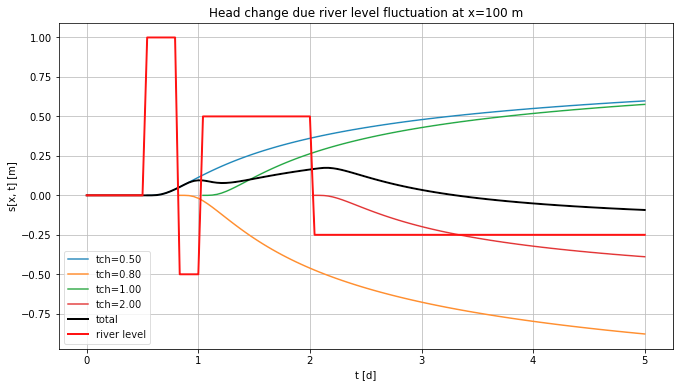
\includegraphics[width=0.8\textwidth]{pictures/Ch6_superpositionInTime_head}
\par\end{centering}
\begin{centering}
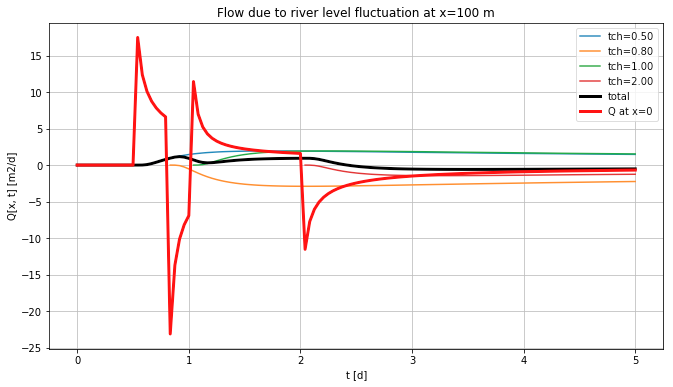
\includegraphics[width=0.8\textwidth]{pictures/Ch6_superpositionInTime_flow}
\par\end{centering}
\caption{\label{fig:Ch6-superposition-in-time-example}Superposition in time
example}
\end{figure}


\section{Groundwater basins as land strips of limited width between straight
head boundaries}

\subsection{\label{subsec:Introduction-5-5-1}Introduction}

In many practical situations, groundwater basins will have a limited
width instead of $x$ extending to infinity. Examples are groundwater
basins that are bounded by a fixed-head boundary on either side. This
includes basins that are closed on one side, because such a line of
no flow is just the water divide, which is equivalent to a symmetrical
basin of double width having the same head boundary on either side.

\begin{figure}
\begin{centering}
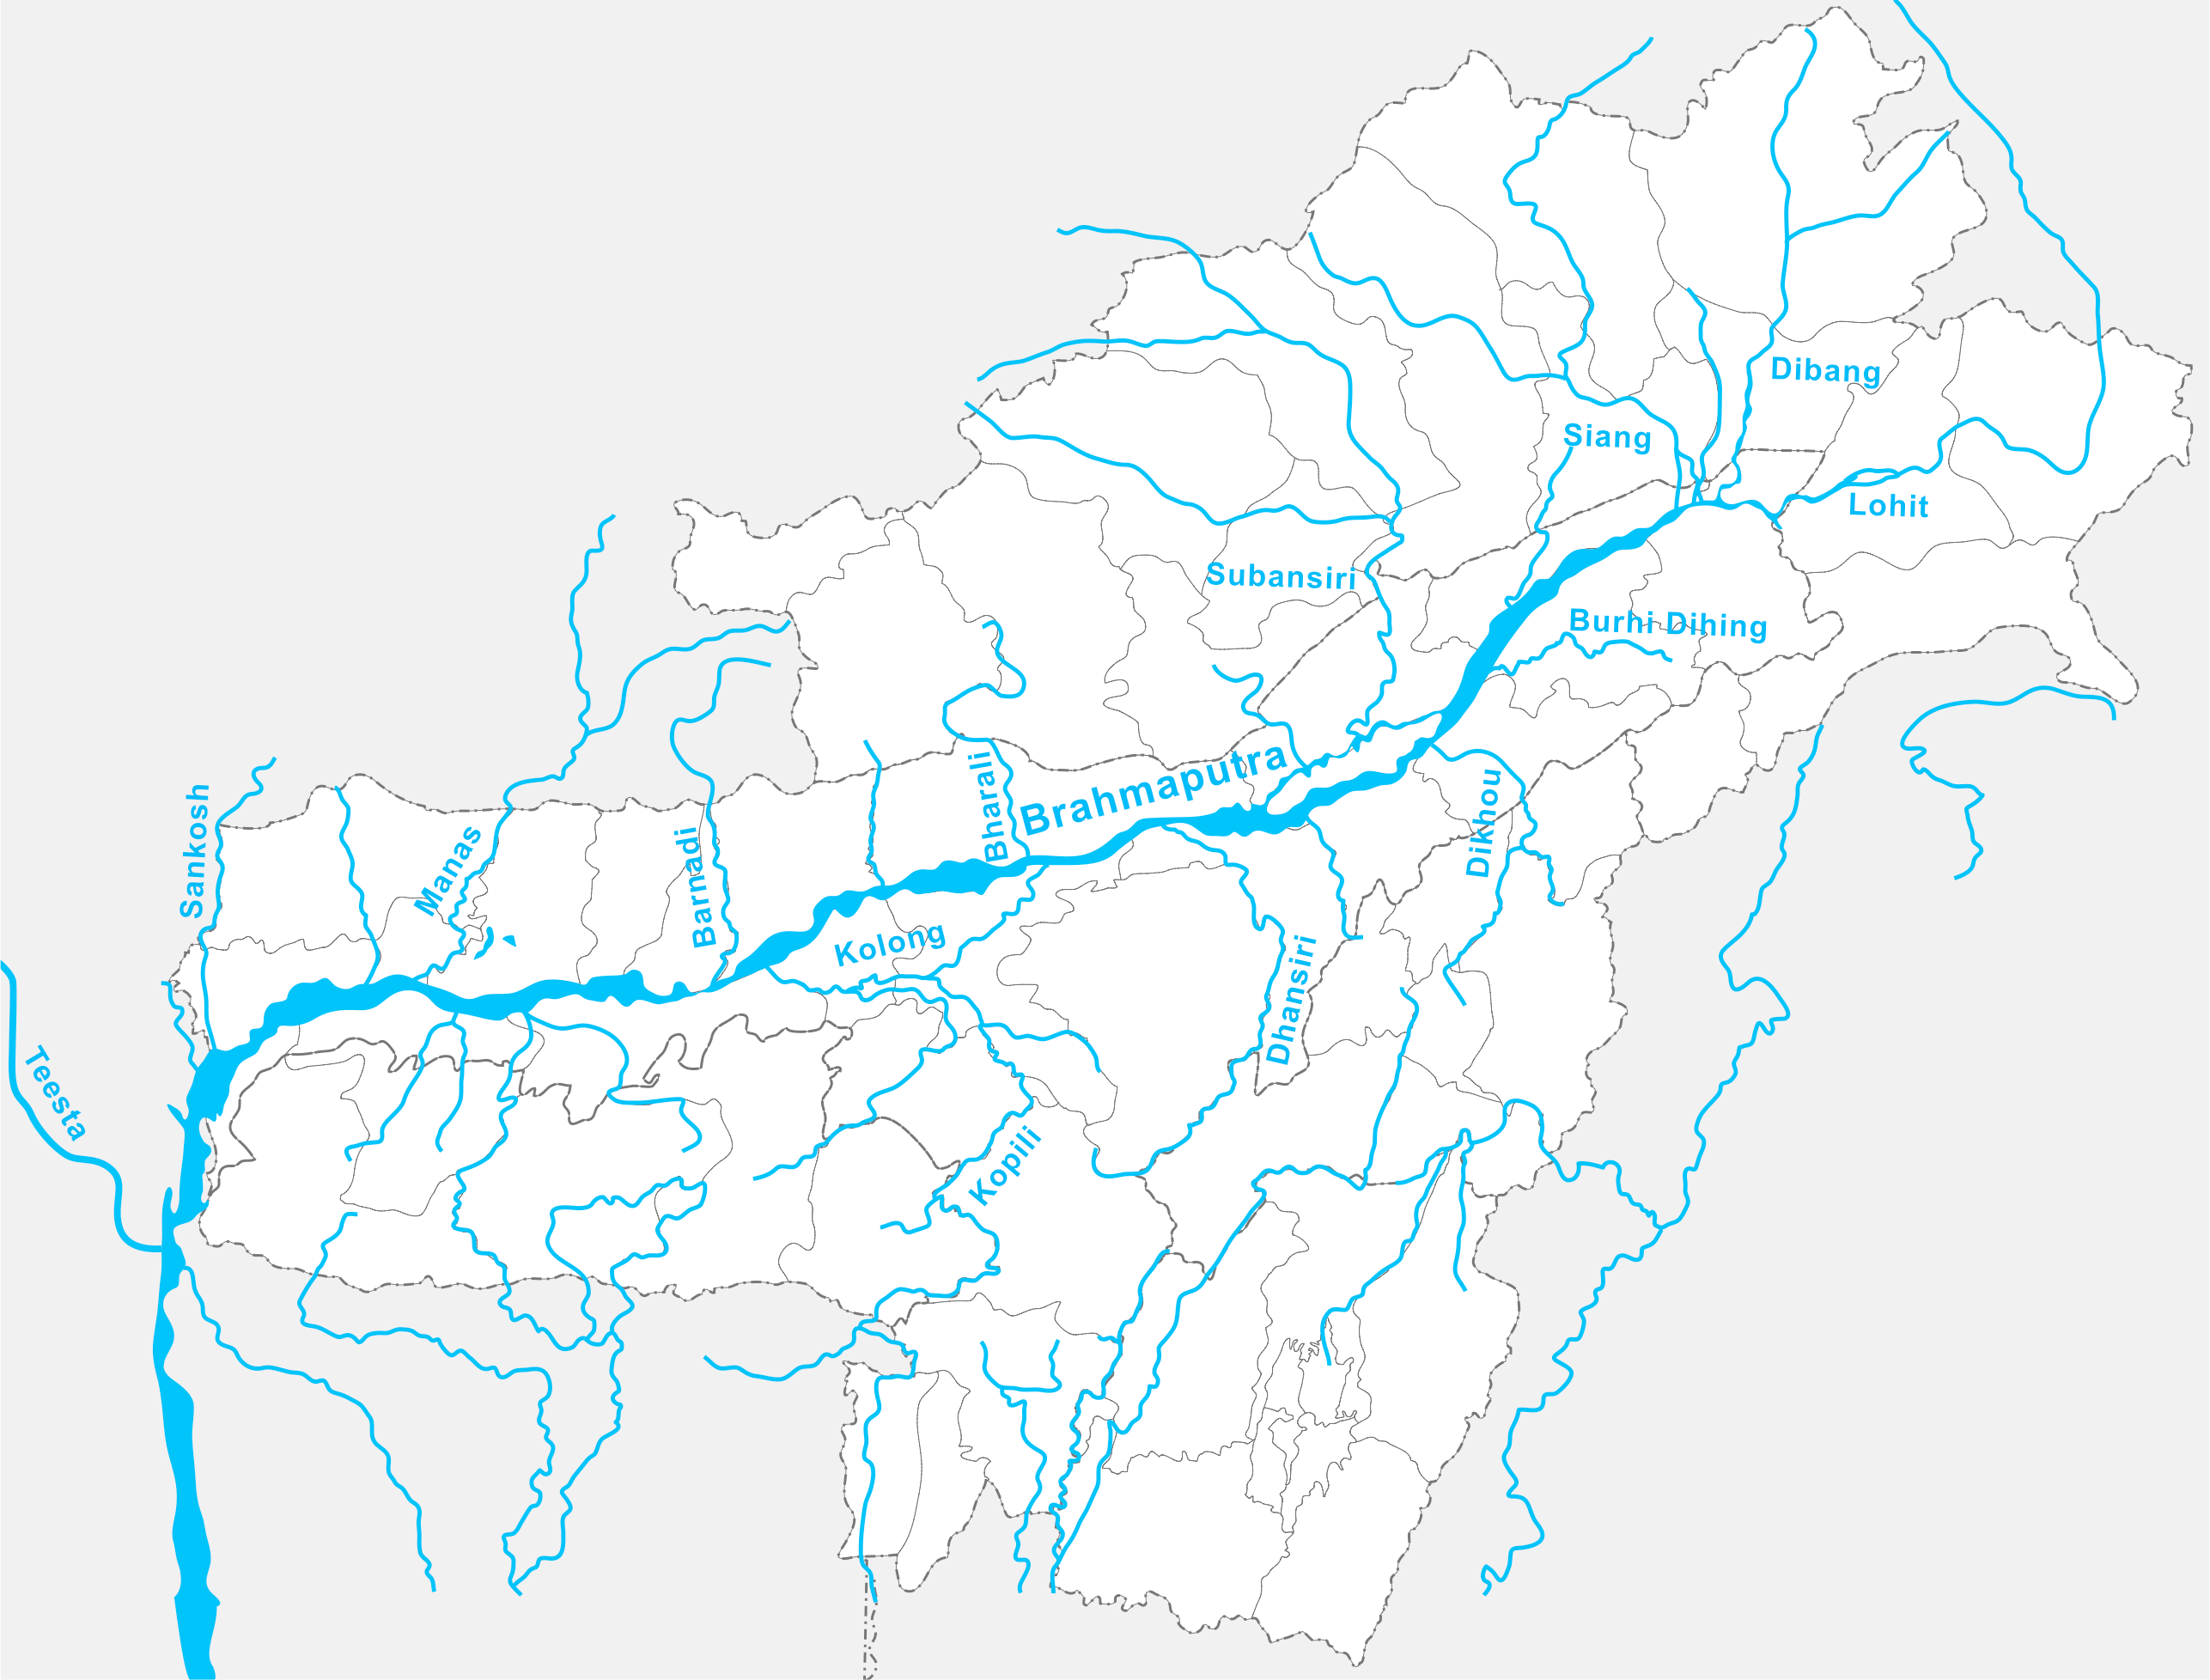
\includegraphics[width=0.8\textwidth]{pictures/BramapuutraRiverBasin}
\par\end{centering}
\caption{\label{fig:Map-of-the-Brahmaputra-basin}Map of the Brahmaputra basin
(Wikipedia)}
\end{figure}

Often, watersheds can be regarded as a set of sub-basins bounded by
river branches on either side of the water divide between them (see
figure  \ref{fig:Map-of-the-Brahmaputra-basin}). The basins considered
here, can be regarded as a simplification of the groundwater system
between two river branches, but also as a parcel of arable land bounded
by two ditches. It's just a matter of scale. The basins considered
here may, therefore, be as narrow as a parcel of arable land or a
meadow between ditches as one can find anywhere in the Netherlands
of perhaps 100 m wide; but they can just as well be a strip of land
land between brooks or tributaries that are several km apart, between
river branches tens of km apart or a desert of which the boundaries
lie at several hundred of km from each other.

Of course, the surface waters bounding most basins are not straight
lines. Nevertheless, we limit ourselves to in this course to basins
that are bounded by two parallel straight head boundaries. This makes
the flow essentially one-dimensional when we ignore resistance due
to vertical flow components with in the aquifer. The latter is very
often justified because the vertical flow components are small compared
to the horizontal ones. If this assumption is not valid like near
a shallow surface-water body, where flow lines bend upward and convergence
causing an extra loss of head, we may always add such effects separately.

In the following sections, we'll learn how to compute the variation
of head and flow in one-dimensional basins (basins in which the only
spatial dimension is $x$ and not $y$ and $z$, that are affected
by the head changes at their two head boundaries, see figure \ref{fig:Head-after-sudden-rise-left-and-right})
which shows such a basin (a strip of land) bounded on either side
by a surface-water body in direct contact with the aquifer, such that
the water level of these surface-water bodies determine the head at
either side of the basin.

We first consider the case where the left-hand boundary head suddenly
rises by a fixed amount $A$ m, while the right-hand boundary head
is kept the constant (see figure \ref{fig:Confined-groundwater-basin-left-rise}).
We will see that maintaining the right-hand head boundary at zero,
requires superposition of the effect of an infinite number of``mirror''
strips of land. After that, we consider a given change of head on
either side of the strip. This case is also solved by by superposition
of an infinite number of equally sized land strips. The case in which
the sudden head change is the same on either side of the land strip
is just a special one. However, it allows us to compare it with a
different general solution describing the drainage of a strip of land
in which the head is initially uniform at a level $A$ above its two
boundaries. Both solutions are equivalent although they look mathematically
completely different. The latter solution, however, allows drastic
simplification when time is large enough and gives us a time constant
that is characteristic of the basin, which allows analyzing time characteristics
of any basin with a simple expression.

The mentioned superposition of an infinite number of strips leads
to superposition patterns that are shown below the respective figure
s. These patterns allow immediate recognition of the correctness of
the superposition pattern required handle the head boundaries on both
ends of the basin or the strip of land we want to analyze.

\subsection{Water level at the left-hand side suddenly rises over a height of
$A$ m, while the water level at the right-hand side remains at zero}

\begin{figure}
\begin{centering}
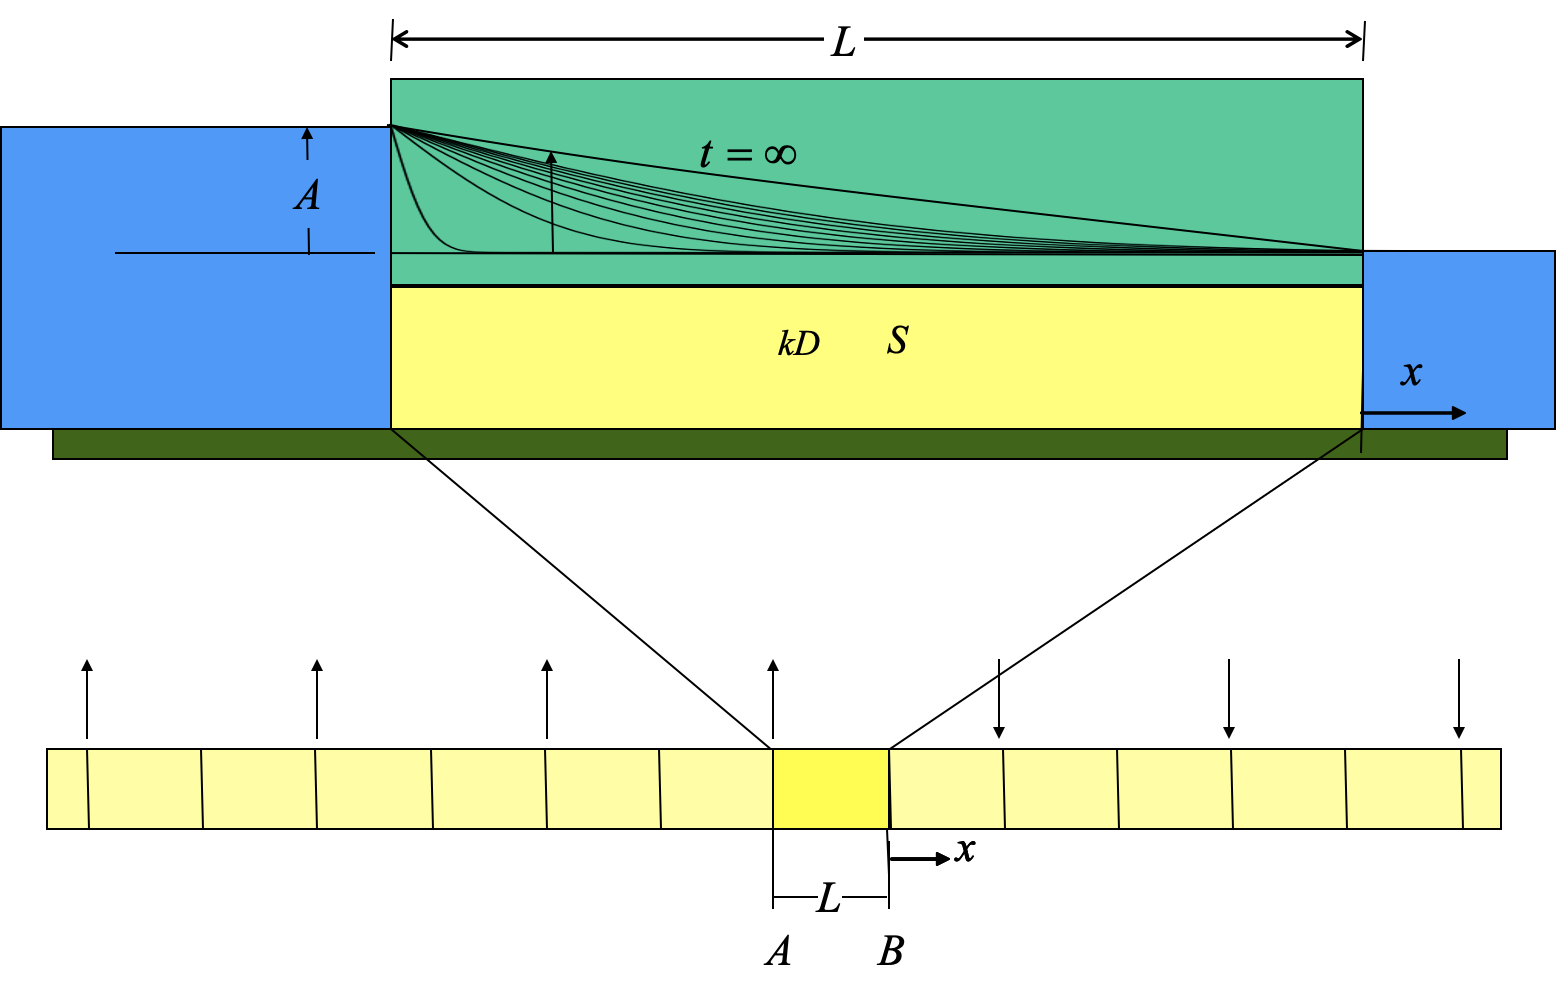
\includegraphics[width=0.8\textwidth]{pictures/StripSuperpositionLeft}
\par\end{centering}
\caption{\label{fig:Confined-groundwater-basin-left-rise}Confined groundwater
basin to the left and right bounded by surface water in direct contact
with the aquifer. Here the water level at the left boundary is suddenly
raised by $A$ m at $t=0$ and that at the right side the surface-water
level remains unchanged at zero. The lower picture shows the superposition
scheme in which the strip of length $L$ between points A and B is
the one to be analyzed. The arrows in the lower picture show where
the water level is suddenly raised or lowered in the mirror scheme.}
\end{figure}

Figure  \ref{fig:Confined-groundwater-basin-left-rise} shows a groundwater
basin with a constant transmissivity $kD$ and storage coefficient
$S$. It has a width $L$ and is bounded on either side by surface
water in direct contact with the confined aquifer. The water level
at the left changes suddenly by an amount $A$. How can we solve this,
given the solution for the half-space (i.e. in which $x$ runs from
0 to $\infty$) that we already have?

The answer is: by superposition by using mirror “ditches”.

The solution for the half-space has been shown before

\[
s\left(x,t\right)=A\,\mathrm{erfc}\left(x\sqrt{\frac{S}{4kDt}}\right)\mbox{, where }x\ge0\mbox{, and }t>0
\]

However, this solution will cause the head at point $B$ to start
rising after some time, while in reality the head should remain 0
at point B. How wan we deal with this mathematically?

When we forget the surface water at $x=B$, but instead assume a ditch
at a distance $L$ to the right of point B, in which the water level
was suddenly lowered at $t=0$ by an amount $A$ m (i.e. changed by
an amount - $A$), then the rising an point B due to the ditch at
$A$ would be exactly counterbalanced (neutralized) by the decline
in point B due to the ditch at a distance $L$ to the right of point
B. As a consequence of both, the head at point B remains zero, which
is exactly the desired effect. In this case, we have one mirror ditch
with opposite head change at distance $L$ to the right of point B.

However, this one mirror ditch does not solve the whole problem, because
after some more time, it will cause the head at point A to start declining,
and so the head at point A would not remain fixed at the value of
$A$ m.

To compensate for that, we need another mirror ditch at distance $2L$
to the left of point A with opposite head change compared to to the
first mirror ditch. But this head change at $2L$ left of point A
will cause the head at $2L$ to the right of point B to change over
time. This requires a mirror ditch at $4L$ to the left of point A
to neutralize this effect. And so on. We will, therefore, end up with
an infinite number of mirror ditches just to make sure that boundary
conditions at both sides of our initial basin are kept that their
desired values.

The lower picture in figure  \ref{fig:Confined-groundwater-basin-left-rise}
intends to make this clear. The darker yellow block represents the
original basin of width $L$. Each arrow represents a mirror ditch
and its direction show whether the water level in it goes up or down.

Is this solution with the shown scheme of mirror ditches correct?
Well, this is. In fact, it's easy to see its correctness at a glance.
Just look at the lower picture in figure  \ref{fig:Confined-groundwater-basin-left-rise}
and consider point B, in which the head should remain zero. As it
should become immediately clear by inspection, each ditch with lowered
water level to the right of point B is exactly canceled at B by each
ditch at the same distance to the left of point B with a rising level.
Hence, the effect in point B of all ditches to the right is exactly
canceled by all ditches to the left of point B. Therefore, the head
at point B remains at zero.

On the other hand, all ditches to the right of point A are exactly
compensated at point A by all ditches to the left of point A, except
for the ditch at point A itself. Hence, the total effect of all the
mirror ditches together at A is zero, so that the only remaining effect
at A is that of the level rise at A itself. That too can be seen at
a glance from the lower picture in figure  \ref{fig:Confined-groundwater-basin-left-rise}.

With respect to the origin of the $x$-axis, it does not matter where
we choose it, we need only to make sure that the distance $x$ in
the formula is correct for each of the mirror wells. In figure  \ref{fig:Confined-groundwater-basin-left-rise},
the point with coordinate $x=0$ was chosen at point $B$, which makes
the mirror ditches symmetrical with respect to this point. The $x$-coordinate
of ditch $i$ to the left is then

\[
-\left(2i-1\right)L
\]
and that of ditch $i$ to the right of point $B$ is

\[
+\left(2i-1\right)L
\]

The (absolute) distance to an arbitrary point with coordinate $x$
is then for the left ditch

\[
\left|x+\left(2i-1\right)L\right|
\]

and to the right ditch

\[
\left|x-\left(2i-1\right)L\right|
\]

We can use these distances directly in the formula that sums the effect
of all wells to yield the net result. This gives for the head change
within the strip of land, where $-L\le x\le0$:

\[
s\left(x,t\right)=A\sum_{i=1}^{\infty}\left\{ \mbox{erfc}\left[\left|x+\left(2i-1\right)L\right|\sqrt{\frac{S}{4kDt}}\right]-\mbox{erfc}\left[\left|x-\left(2i-1\right)L\right|\sqrt{\frac{S}{4kDt}}\right]\right\} 
\]
and doing the same for the for the discharge expression, yields

\[
Q\left(s,t\right)=A\sqrt{\frac{kDS}{\pi t}}\,\sum_{i=1}^{\infty}\left\{ \mbox{exp}\left[-\left(x+\left(2i-1\right)L\right)^{2}\frac{S}{4kDt}\right]+\mbox{exp}\left[\left(x-\left(2i-1\right)L\right)^{2}\frac{S}{4kDt}\right]\right\} 
\]

Note that the second term in the formula for $s\left(x,t\right)$
has a minus sign because of the water level in the right-hand ditches
was lowered. However, the second term in the formula for the discharge
$Q\left(s,t\right)$ has a plus sign, because both the left-hand and
the right-hand ditches cause a positive flow, i.e. a flow in the positive
direction of the $x$-axis.

When you implement this scheme in Python, make sure you start the
sum (loop) with $i=1$ and not $i=0$.

Figure  \ref{fig:StripLeftHandRise} shows the results for several
times. Because the point $x=0$ was chosen to be at the point B at
the right-hand side of the strip, the $x$-values within the strip
are now negative. Also notice that the steady-state solution, which
is reached after about 3 days, has a head that declines linearly from
2.5 m at the left to 0 at the right of the strip. The discharge $Q$
through the aquifer, therefore, must equal $Q=A/L\times kD=2.5/250\times600=6$
m$^{2}$/d. This is indeed the case all along the width of the strip
as can be seen in figure  \ref{fig:StripLeftHandRise}.

\begin{figure}
\begin{centering}
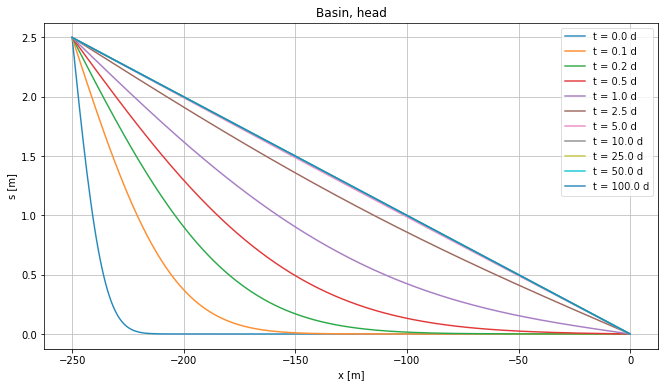
\includegraphics[width=0.8\textwidth]{pictures/stripHeadLeftRise}
\par\end{centering}
\begin{centering}
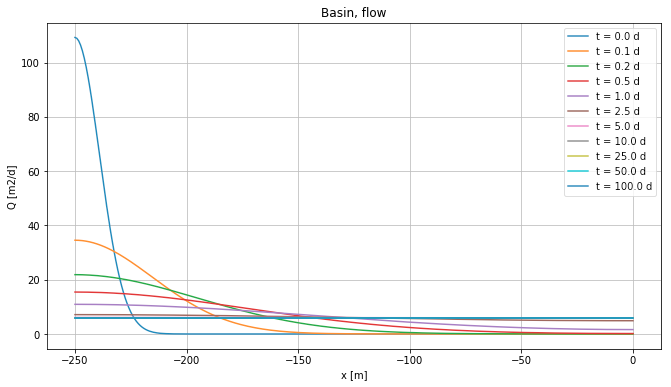
\includegraphics[width=0.8\textwidth]{pictures/stripHeadLeftRise_Q}
\par\end{centering}
\caption{\label{fig:StripLeftHandRise}Top: head. Bottom: flow. After sudden
head rise of $A=2.5$ m for various times, $L=250$ m, $kD=600\,\mathrm{m^{2}/d}$,
$Sy=0.1$}
\end{figure}


\paragraph{Shifting the zero point of the $x$-axis}

We may choose any point as the origin of the x-axis. Let's put it
at a distance $a$ to the right of point A. The the coordinate of
ditch $i$ to the left would be $x_{i}=-2iL-a$ for $0\le i<\infty$
and that of ditch $i$ to the right would be $x_{i}=2iL-a$ for $1\le i<\infty$.
So that the distance between the first well a the right $\left(i=1\right)$
and the first well at the left $\left(i=0\right)$ equals

\[
d=-a-\left(-2L-a\right)=2L
\]

So with this zero point for the x-axis we can write the superposition
as follows (note the start of the summation differs (1 at the left
one and 0 at the right one)

\begin{eqnarray*}
s\left(x,t\right) & =\\
 &  & A\left\{ \sum_{i=0}^{\infty}\mbox{erfc}\left[\left|x-(-2iL-a)\right|\sqrt{\frac{S}{4kDt}}\right]-\sum_{i=1}^{\infty}\mbox{erfc}\left[\left|x-\left(2iL-a\right)\right|\sqrt{\frac{S}{4kDt}}\right]\right\} 
\end{eqnarray*}

removing needless minus signs in the distances

\begin{eqnarray*}
s\left(x,t\right) & =\\
 &  & A\left\{ \sum_{i=0}^{\infty}\mbox{erfc}\left[\left|x+a+2iL\right|\sqrt{\frac{S}{4kDt}}\right]-\sum_{i=1}^{\infty}\mbox{erfc}\left[\left|x+a-2iL\right|\sqrt{\frac{S}{4kDt}}\right]\right\} 
\end{eqnarray*}


\subsection{Arbitrary non-symmetrical case}

Now consider the general case, in which the head at the left and right
change by different values. Again, we need mirror ditches. This time
not only to fix the left-hand head at the desired level, but also
the right-hand head. Of course, you can regard this case from the
perspective of the problem that we just solved. It is then the sum
of the case in which the left-hand level was raised by $A$ m and
the right-hand level was kept at zero and the same case of which the
right-hand size was raised by $B$ m and the left-hand side was kept
at zero.

\begin{figure}
\begin{centering}
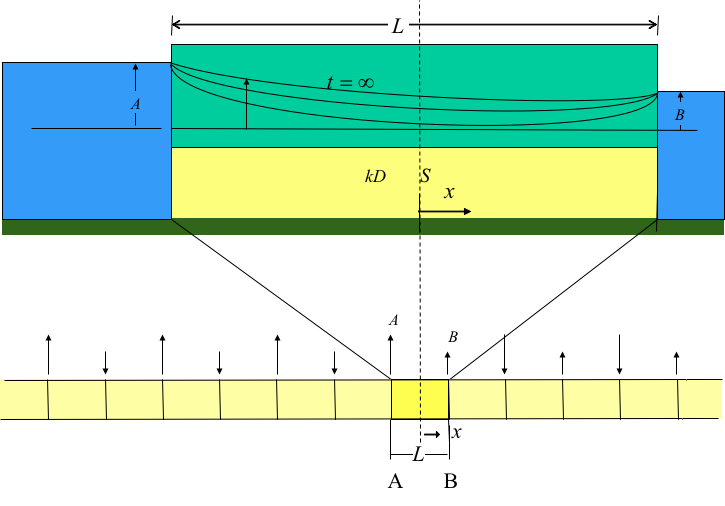
\includegraphics[width=0.8\textwidth]{pictures/StripSuperpositionLeftRight_picture}
\par\end{centering}
\caption{\label{fig:Strip-left-riseby-a-right-by-b}As figure \ref{fig:Confined-groundwater-basin-left-rise}
but the water level is raised independently on the left and right
side by $A$ and $B$ respectively, and the $x$-axis is now centered
in the center of the strip. The lower picture shows the superposition
scheme; the arrows show where the water level is suddenly raised or
lowered.}
\end{figure}

But let's just solve it, after taking the $x=0$ at a convenient location,
which would be in the center. Note however, you can put it at another
location, but then the formulas change accordingly.

The image at the bottom of figure  \ref{fig:Strip-left-riseby-a-right-by-b}
shows the strip and the mirror ditches. By looking at this picture,
it should immediately be clear that this scheme of mirror ditches
is correct. To see this, look at point A. You will then notice that
each ditch to the left of A is compensated exactly by each ditch at
the right of A. Therefore, the only effect of all the ditches at point
A, including the ditch at pint A itself, is that of the ditch at point
A itself; all others cancel at point A. Next focus on point B and
notice that this is also true for point B. Hence, at point A, the
only effect that remains is that of the head change in the ditch at
point A, and at point B, the only effect that remains at point B is
that o the head change of the ditch at point B.

With this in mind, it becomes straightforward to write the expression
for the head within the strip of land. To do that, just consider a
point $x$ and write the distance to all the ditches in terms of strip
width $L$ and $x$. Doing this, we get

\begin{eqnarray*}
s\left(x,t\right) & = & \dots
\end{eqnarray*}

\[
A\,\sum_{i=1}^{\infty}\left\{ \mbox{erfc}\left[\left\{ \left(2i-1\right)L-\frac{L}{2}+x\right\} \sqrt{\frac{S}{4kDt}}\right]-\mbox{erfc}\left[\left\{ \left(2i-1\right)L+\frac{L}{2}-x\right\} \sqrt{\frac{S}{4kDt}}\right]\right\} +\dots
\]

\[
\dots+B\,\sum_{i=1}^{\infty}\left\{ \mbox{erfc}\left[\left\{ \left(2i-1\right)L-\frac{L}{2}-x\right\} \sqrt{\frac{S}{4kDt}}\right]-\mbox{erfc}\left[\left\{ \left(2i-1\right)L+\frac{L}{2}+x\right\} \sqrt{\frac{S}{4kDt}}\right]\right\} 
\]

Like it was done above, a similar expression can be written down for
the flow $Q$.

An example result is shown in figure  \ref{fig:Head-after-sudden-rise-left-and-right}
for the case where at $t=0$ the head at the left boundary was raised
by $A=2.5$ m and at the right side by $B=1.5$ m. Again, a steady
state is reached after about 5 days, the flow is then constant, i.e.
$\left(A-B\right)/L\times kD=1/250\times600=2.5$ m $^{2}$/d. The
flows are initially, for a short period, high and opposite on both
sides of the strip. Later on it became constant from left to right.

\begin{figure}
\begin{centering}
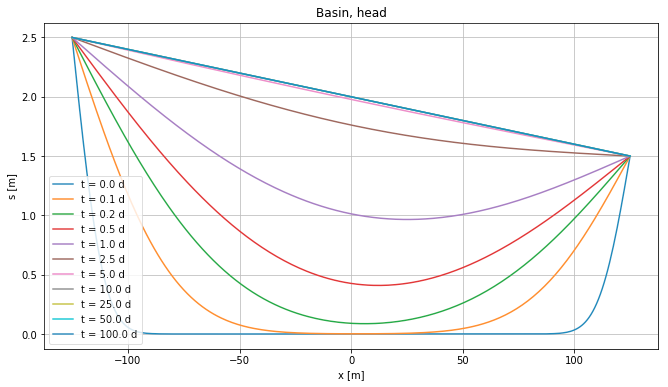
\includegraphics[width=0.8\textwidth]{pictures/StripSuperpositionLeftRight}
\par\end{centering}
\begin{centering}
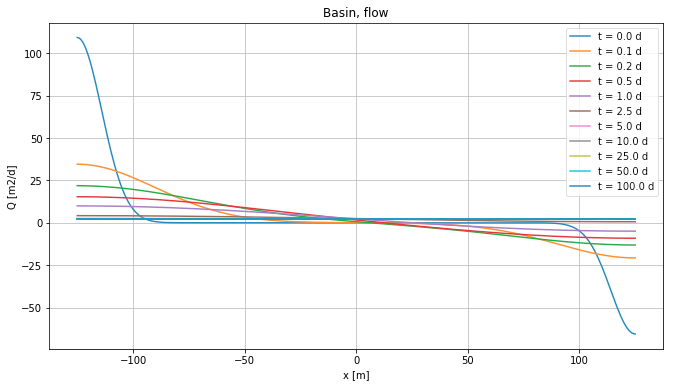
\includegraphics[width=0.8\textwidth]{pictures/StripSuperpositionLeftRight_Q}
\par\end{centering}
\caption{\label{fig:Head-after-sudden-rise-left-and-right} Top: head Bottom:
flow. After sudden head rise by $A=2.5$ m at $x=-L/2$ and $B=1.5$m
at $x=+L/2$ for various times, $kD=600\,\mathrm{m^{2}/d}$, $Sy=0.1$,
$L=250$ m.}
\end{figure}


\subsection{Symmetrical case, $A=B$}

The symmetrical case is obtained when the rise of the water level
at the left-hand boundary is the same as that at the right-hand boundary,
so $A=B$. Of course, this case is included in the former one. However,
we'll still work it out as we need it in the next section to compare
it with a completely different expression for the same case that we'll
use to generalize our understanding of the transient characteristics
of groundwater basins.

\begin{figure}
\begin{centering}
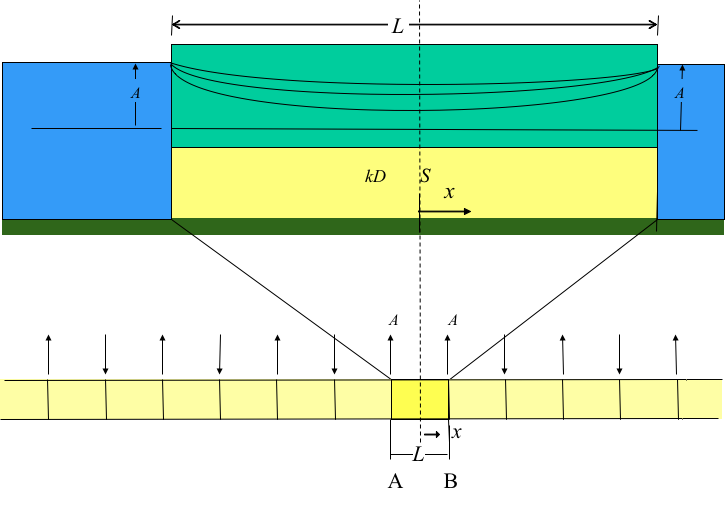
\includegraphics[width=0.8\textwidth]{pictures/StripSuperpositionSymmetrical}
\par\end{centering}
\caption{\label{fig:Groundwater-basin-symmetrical}Groundwater basin bounded
by surface water in direct contact on either side in which the water
level is raised by $A$ on both sides. The lower picture shows the
superposition scheme with the errors indicating where the water level
is raised or lowered for the superposition.}
\end{figure}

figure  \ref{fig:Groundwater-basin-symmetrical} shows the situation.
It's the same as before, but the rise is now $A$ m on both sides,
which simplifies the expression to a sum over two terms instead of
four terms.

Taking $x=0$ conveniently at the center of the strip like before,
we can draw the mirror scheme. This is was done in the lower picture
of figure  \ref{fig:Groundwater-basin-symmetrical}. Like before,
by first focusing on the symmetry around point A and then on the symmetry
around point B, you should see at a glance that this mirror scheme
is correct. Knowing the mirror scheme, we can write the expression
(See also Carslaw and Jaeger, p97, eq 9):

\begin{align}
s\left(x,t\right) & =A\,\sum_{i=1}^{\infty}\label{eq:sSuddenRiseOnBothSides}\\
 & \left\{ \left(-1\right)^{i-1}\left[\mbox{erfc}\left(\left[\left(i-\frac{1}{2}\right)L+x\right]\sqrt{\frac{S}{4kDt}}\right)+\mbox{erfc}\left(\left[\left(i-\frac{1}{2}\right)L-x\right]\sqrt{\frac{S}{4kDt}}\right)\right]\right\} 
\end{align}

The factor $\left(-1\right)^{i-1}$ is just a series $+1,-1,+1,-1,+1,-1,\dots$
because the direction of the arrow alternates with each further ditch
on both sides.

\paragraph{Another perspective, drainage of a basin in which the head is initially
at distance A above the fixed heads at either side of the strip}

This case, in which the water level at both boundaries suddenly rises
by the same amount of $A$ m, can also be regarded as a transient
drainage after a heavy shower of rain on the strip. If we assume that
the rain surplus $P$ {[}m{]} reaches the water table immediately,
then the water level in the entire strip would suddenly rise by the
amount $A=\frac{P}{S_{y}}$ in which $P$ is the rain (that part of
it that reaches the water table) and $S_{y}$ is the specific yield.
Therefore, after such a shower, the head in the entire strip would
suddenly be at $A$ m above the water level in the ditches on either
side. Immediately after this shower, assumed to be of zero duration,
the strip starts draining. The picture that is thus obtained is the
same as that in which the ditches suddenly rise by $A$ m at $t=0$,
be it that the drainage picture is turned upside-down. This drainage
situation is illustrated in figure  \ref{fig:Symmetrical-strip-draining}.

\begin{figure}
\begin{centering}
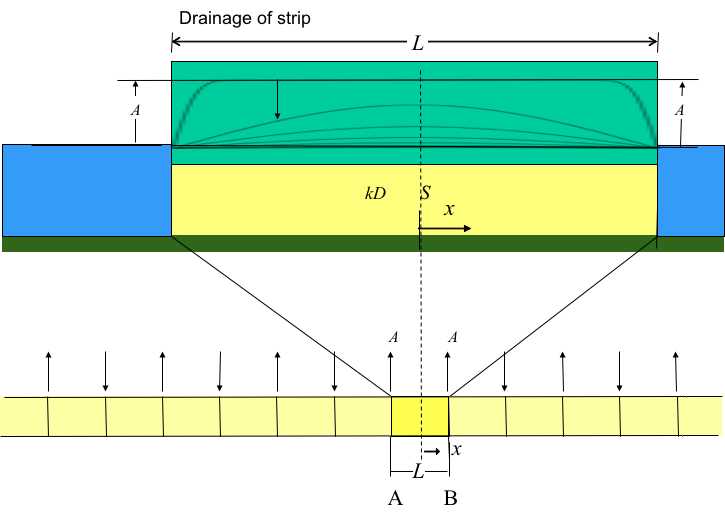
\includegraphics[width=0.8\textwidth]{pictures/StripSuperpositionSymmetricalDrainage}
\par\end{centering}
\caption{\label{fig:Symmetrical-strip-draining}Symmetrical strip draining
after heavy shower.}
\end{figure}

To use this equation to compute the drainage of a groundwater basins
one may write $s\left(x,t\right)=A\left(1-\sum\dots\right)$, where
$\sum\dots$ is the entire expression in the formula above.

The discharge at any point $x$ is obtained as usual by inserting
using Darcy's law, i.e. $Q=-kD\left(\partial s/\partial x\right)$:

\begin{eqnarray*}
Q\left(x,t\right) & = & -A\,\left(\sqrt{\frac{kDS_{y}}{\pi t}}\right)\sum_{i=1}^{\infty}\left(-1\right)^{i-1}\\
 &  & \left[\exp\left(-\left[\left(i-\frac{1}{2}\right)L+x\right]^{2}\frac{S}{4kDt}\right)-\exp\left(-\left[\left(i-\frac{1}{2}\right)L-x\right]^{2}\frac{S}{4kDt}\right)\right]
\end{eqnarray*}

\begin{equation}
\dots\label{eq:QsuddenRiseOnBothSides}
\end{equation}

As can be seen from figure  \ref{fig:Head-after-sudden-rise-left-and-right},
immediately after the head change, the water table drops very fast
near the edges of the strip. Very soon, however, the head takes the
shape of a cosine and the strip drains gradually until its final equilibrium
at $s\left(x,t\rightarrow\infty\right)=0$ is reached.

The cosine shape at later drainage stages follows from another form
of analytical solution of the same strip, which will be discussed
in the next section.

An example is shown in figure  \ref{fig:Head-after-sudden-rise-same-at-both-sides}.
In this case, the time interval between times used to show the heads
is the so-called halftime as will be derived later. After each halftime,
the difference between the head and the equilibrium final head is
halved.

\begin{figure}
\begin{centering}
\includegraphics[width=0.8\textwidth]{pictures/StripSuperpositionSymmetrical_h}
\par\end{centering}
\begin{centering}
\includegraphics[width=0.8\textwidth]{pictures/StripSuperpositionSymmetrical_Q}
\par\end{centering}
\caption{\label{fig:Head-after-sudden-rise-same-at-both-sides}Top: head. Bottom:
flow. Drainage after a sudden shower of 100 mm, such that with $S=0.1$,
$A=1$ m at $t=0+$. Thereafter, the strip drains towards the surface
water at both sides, the water level of which is kept constant. $kD=600\,\mathrm{m^{2}/d}$,
$S=0.1$, $L=250$ m. Situation for several times.}
\end{figure}


\subsection{\label{subsec:Questions-5-5-5}Questions}
\begin{enumerate}
\item Set up a mirror scheme for the case of a strip of land bounded by
straight surface water on either side, where the surface water stage
of the right-hand side canal suddenly changes by a fixed value.
\item Show, explain on the hand of the obtained mirror scheme that the result
is correct, i.e. that the result with all the mirror strips match
the boundary conditions exactly.
\item What would be the mirror scheme for the strip if the right-hand boundary
was closed?
\end{enumerate}

\section{\label{sec:Symmetrical-drainage-from-charcteristic-time}Symmetrical
drainage from a land strip bounded by straight head boundaries (characteristic
time of flow basins)}

Here we introduce a solution for the drainage of a land strip that
initially has uniform head $s\left(0,x\right)=A$ and is bounded by
two straight head boundaries at $x=\pm b$ with head at $s\left(\pm b,t\right)=0$.
This solution looks completely different from the one we obtained
by infinite mirroring of strips of land as we did in the previous
sections, yet it provides the same result for the symmetrical case.
The advantage of this form of the solution is that it can be further
analyzed to deduce general drainage patterns and their time scale.

\subsection{\label{subsec:Analytical-solution}Analytical solution}

An analytical solution for the drainage of a strip of land that we
solved by superimposing an infinite number of mirror ditches is also
known in a completely different mathematical form published by \textcite{Carslaw1986},
p97, eq. 8. It was also published by \textcite{Verruijt1999}, p87
and is widely known in the Netherlands as``Kraaijenhoff van der Leur''.
It reads

\begin{equation}
s\left(x,t\right)=A\,\frac{4}{\pi}\sum_{j=1}^{\infty}\left\{ \frac{\left(-1\right)^{j-1}}{2j-1}\cos\left[\left(2j-1\right)\left(\frac{\pi}{2}\right)\frac{x}{b}\right]\exp\left[-\left(2j-1\right)^{2}\left(\frac{\pi}{2}\right)^{2}\frac{kD}{b^{2}S}t\right]\right\} \label{eq:Kraaijenoff-van-der-Leur-Verruijt}
\end{equation}
From this we obtain the flow by setting $Q=-kD\frac{\partial s}{\partial x}$.
This yields

\[
Q\left(x,t\right)=+2\,kD\,\frac{A}{b}\,\sum_{j=1}^{\infty}\left\{ \left(-1\right)^{j-1}\sin\left[\left(2j-1\right)\left(\frac{\pi}{2}\right)\frac{x}{b}\right]\exp\left[-\left(2j-1\right)^{2}\left(\frac{\pi}{2}\right)^{2}\frac{kD}{b^{2}S}t\right]\right\} 
\]

As always, $s\left(x,t\right)$ is the head relative its equilibrium
value, which is $s\left(x,\infty\right)=0$. The $x$-axis is taken
such that $x=0$ in the center and $x\pm b$ corresponds to the sides
with fixed boundary conditions $s\left(\pm b,t\right)=0$. The initial
head is $s\left(x,0\right)=A$ inside the section, $-b<x<b$. The
formula describes the drainage that follows after the initial situation.

This behavior is characteristic for a basin after a sudden shower
causing the head in it to suddenly rise everywhere by the same amount,
while the level in the ditches at both sides is kept the same. After
the shower, the drainage sets in and gradually continues until equilibrium
is finally reached (which theoretically takes infinite time).

Equation \ref{eq:Kraaijenoff-van-der-Leur-Verruijt} yields the same
head as was obtained previously with superposition of an infinite
number of erfc-functions, even though the solution presented here
looks mathematically completely different. We will use this solution
to derive drainage characteristics that can be applied in practice
on different scales.

Figure  \ref{fig:Head-after-sudden-rise-includes-Kraaijenhof} gives
the results as an example. The lines are the same as in figure \ref{fig:Head-after-sudden-rise-same-at-both-sides}
and the dots are the results of equation \ref{eq:Kraaijenoff-van-der-Leur-Verruijt}
for the same times. The results are, obviously, the same. The lower
picture in this figure  shows the computed discharge using both approaches.

\begin{figure}
\begin{centering}
\includegraphics[width=0.8\textwidth]{pictures/stripSymetricWithKraaijenhof}
\par\end{centering}
\begin{centering}
\includegraphics[width=0.8\textwidth]{pictures/stripSymetricWithKraaijenhof_Q}
\par\end{centering}
\caption{\label{fig:Head-after-sudden-rise-includes-Kraaijenhof}Top: head.
Bottom: flow. Free drainage of basin from initial head at $A=1$ m
for various times, $kD=600\,\mathrm{m^{2}/d}$, $Sy=0.1$, $L=250$
m. Drawn lines were computed with the $\mbox{erfc}$-functions and
are the same as in figure \ref{fig:Symmetrical-strip-draining}; the
dots were computed with equation \ref{eq:Kraaijenoff-van-der-Leur-Verruijt}.
The lines from both approaches completely overlap.}
\end{figure}

Finally, figure  \ref{fig:Kraaijenhoff-individual-terms} shows a
graph of the individual terms of the series in equation \ref{eq:Kraaijenoff-van-der-Leur-Verruijt}
for head and for discharge $Q$, both together with the total solution
obtained by the summation a large number of terms.

\begin{figure}
\begin{centering}
\includegraphics[width=0.8\textwidth]{pictures/Kraaijenhoff_individual_terms_h}
\par\end{centering}
\begin{centering}
\includegraphics[width=0.8\textwidth]{pictures/KraaijenhoffInvidualTerms_Q}
\par\end{centering}
\caption{\label{fig:Kraaijenhoff-individual-terms}Showing the individual terms
of the series in equation \ref{eq:Kraaijenoff-van-der-Leur-Verruijt}
for head and for flow together with the total solution obtained by
the summation. This is done for $t=0.0073$ d. Other values are the
same as in figure \ref{fig:Head-after-sudden-rise-includes-Kraaijenhof}.}
\end{figure}


\paragraph{Exercise:}

Implement equation \ref{eq:Kraaijenoff-van-der-Leur-Verruijt} yourself
together with the solution using superposition of mirror ditches and
show that the outcomes are the same when simulation free drainage
of a strip of land. You should obtain figure  \ref{fig:Head-after-sudden-rise-includes-Kraaijenhof}.

\subsection{\label{subsec:Long-term-drainage-behavior-drainage}Long-term drainage
behavior, characteristic drainage time}

Equation \ref{eq:Kraaijenoff-van-der-Leur-Verruijt} looks complicated
at first, but it can be broken down to yield useful and practical
insights pertaining to the dynamic characteristics of draining groundwater
basins. For that purpose, we analyze the expression under the summation.

The $2j-1$ is just the series $1,3,5,7,\dots$. and $\left(-1\right)^{2j-1}=+1,-1,+1,-1,\dots$.
Next, we have a product of a cosine and an exponent. The cosine will
fluctuate between -1 and +1 and it only depends on $x$. Then notice
the exponent, which only depends on time. For simplicity write it
as

\[
\exp\left[-\left(2j-1\right)^{2}\left(\frac{\pi}{2}\right)^{2}\frac{t}{T}\right]
\]
where $T=\frac{b^{2}S}{kD}$. $T$ may thus be regarded as a characteristic
time of the drainage. The exponent terms in the series now become

\[
\exp\left(-\left(\frac{\pi}{2}\right)^{2}\frac{t}{T}\right),\,\exp\left(-9\left(\frac{\pi}{2}\right)^{2}\frac{t}{T}\right),\,\exp\left(-25\left(\frac{\pi}{2}\right)^{2}\frac{t}{T}\right),\,\dots
\]

Because $\frac{t}{T}>0$, the second and higher terms will finally
become much smaller than the first and may, therefore, be neglected
when $t>t_{n}=nT$ where $n$ needs to be estimated. So let us see
when the second term becomes much less than the first one, so that
only the first term matters and we can neglect all higher terms. Therefore,
compare the first term with the second and demand that it's much larger
than the second:

\[
\exp\left(-\pi^{2}\frac{t}{T}\right)\gg\exp\left(-9\pi^{2}\frac{t}{T}\right)
\]
or

\[
\exp\left(-\left(\frac{\pi}{2}\right)^{2}\frac{t}{T}\right)=G\,\exp\left(-9\left(\frac{\pi}{2}\right)^{2}\frac{t}{T}\right)
\]
where $G$ is just a large positive number. We may choose $G=100$,
which means, we neglect all higher terms, when the first term is at
least 100 times a large as the second.

Taking the logarithm at both sides of the equal-sign yields

\[
-\left(\frac{\pi}{2}\right)^{2}\frac{t}{T}=\ln G-9\left(\frac{\pi}{2}\right)^{2}\frac{t}{T}
\]
Hence, we obtain

\[
8\left(\frac{\pi}{2}\right)^{2}\frac{t}{T}=\ln G
\]
so that

\[
\frac{t}{T}=\frac{\ln G}{8\left(\frac{\pi}{2}\right)^{2}}=\frac{\ln100}{8\left(\frac{\pi}{2}\right)^{2}}\approx0.23
\]

This way, for the chosen value of $G=100$, we find $t=0.23T$. Therefore,
we conclude that all higher terms are negligible when $t>0.23\,T$.
Of course, we could also have chosen another large value of $G$,
but the outcome would not be much different because $G$ is under
the logarithm.

This means that when $t>0.23T$ the expression given above reduces
to only one term

\[
s\left(x,t\right)=A\frac{4}{\pi}\cos\left(\frac{\pi}{2}\frac{x}{b}\right)\exp\left(-\left(\frac{\pi}{2}\right)^{2}\frac{t}{T}\right)\mbox{, with }t>0.23T\mbox{, and }T=\frac{b^{2}S}{kD}
\]

This is a simple-to-understand expression. It is a cosine that only
depends on $x$, not on time, with its top equal to $\frac{4}{\pi}A$
in the center where $x=0$ and zero where $x=\pm b$. This cosine-shaped
groundwater mound gradually declines according to the exponent that
only depends on time, not in $x$.

An exponential decline can always be characterized by its so-called
halftime. The halftime is the time in which the head reduces by a
factor 0.5. So if $t$ increases by one halftime, $\Delta t_{50\%}$,
the head $s(x,t)$ is reduced to $0.5\times s\left(x,t\right)$.

To obtain this halftime, just write down mathematically that half
the head at time $t$ is obtained at time $t+\Delta t_{50\%}$. So
literally

\[
0.5\exp\left(-\left(\frac{\pi}{2}\right)^{2}\frac{t}{T}\right)=\exp\left(-\left(\frac{\pi}{2}\right)^{2}\frac{t+\Delta t_{50\%}}{T}\right)
\]
Taking the logarithm on both sides yields

\[
\ln0.5-\left(\frac{\pi}{2}\right)^{2}\frac{t}{T}=-\left(\frac{\pi}{2}\right)^{2}\frac{t+\Delta t_{50\%}}{T}
\]
and so

\begin{eqnarray*}
\ln0.5 & = & -\left(\frac{\pi}{2}\right)^{2}\frac{\Delta t_{50\%}}{T}
\end{eqnarray*}
and, therefore,

\[
\frac{\Delta t_{50\%}}{T}=\left(\frac{2}{\pi}\right)^{2}\ln2\approx0.28
\]

or

\[
\Delta t_{50\%}\approx0.28T\mbox{, where }T=\frac{b^{2}S}{kD}
\]

This implies that when time progresses by $\Delta t_{50\%}=0.28T$,
the drawdown is halved (under the condition that $t>0.23T$ when all
higher terms can be neglected).

This result allows us to immediately compare the halftimes of the
free drainage of groundwater basins of widely different sizes and
with widely different aquifer properties. Let the size of the basin
be expressed by its representative half-width $b$. Of course, when
a groundwater basin does not have has the shape of a long strip bounded
by two straight canals, one should estimate a reasonable half-width
based on the distance from the water divide to its drainage base,
be it ditches, canals, streams, lakes, rivers or the coast.

Table \ref{tab:Charactersitic-times-of-various-groundwater-basins}
gives the characteristic time $T=b^{2}S/kD$ and the halftime $\Delta t_{50\%}=0.28T$
for some groundwater basins. This table illustrates, that different
groundwater basins that may have similar transmissivities and storage
coefficients, may still have extremely large differences in half times
or characteristic times. Especially the effect of the width of the
basins, $b$, is large because it works to the power 2 in $T=b^{2}S/kD$.
This way, a simple meadow or arable field in the Netherlands bounded
between two ditches just 100 m apart may have a halftime in the order
of one day, but large systems, notably deserts, like the Kalahari
may have a halftime in the order o 10000 years. This implies that
the small meadow in the Netherlands, will hardly remember the rain
shower that fell one week ago, while the Kalahari is still draining
the water that it collected during previous wet episodes may thousands
of years ago, like the last ice age. Recent research with respect
to the world's largest aquifer, the Nubian sandstone, showed that
this aquifer, which extends over much of Sudan, Egypt and Libya, may
be regarded as a water-table aquifer that is still slowly draining
the water that it collected during wet episodes when the Sahara was
still wet (especially between the beginning of the Holocene era until
about 4600 years ago, \parencite{Powell2015,Voss2014} and that the
current oases represent the last remains of the water table reaching
above ground surface, and which was much higher thousands of years
ago.

\begin{table}
\caption{\label{tab:Charactersitic-times-of-various-groundwater-basins}Characteristic
times $T=b^{2}S_{y}/kD$ and halftimes $\Delta t_{50\%}=0.28T$ of
the drainage of various groundwater systems}

\begin{tabular}{|c|c|c|c|c|c|c|c|c|}
\hline 
Situation & Country & $kD\mathrm{[m^{2}/d]}$ & $Sy$ & $b\mathrm{[m]}$ & $T\mathrm{[d]}$ & $T_{50\%}%\mathrm{[d]}
$ & $T\mathrm{[yr]}$ & $T_{50\%}%\mathrm{[yr]}
$\tabularnewline
\hline 
\hline 
Nubian Sandstone & Egypt & 500 & 0.001 & 500,000 & 500,000 & 140,000 & 3845 & 420\tabularnewline
\hline 
Kalahari Desert & Botswana & 500 & 0.1 & 300,000 & $18\times10^{6}$ & 540,000 & 14000 & 15000\tabularnewline
\hline 
Veluwe Area & NL & 6,000 & 0.27 & 20,000 & 18,000 & 5,040 & 14 & 15\tabularnewline
\hline 
Dunes (NL coast) & NL & 200 & 0.11 & 2,000 & 4,400 & 1,200 & 3 & 4\tabularnewline
\hline 
Flower bulb fields & NL & 200 & 0.1 & 50 & 1.25 & 0.35 & 0.001 & 0.001\tabularnewline
\hline 
\end{tabular}
\end{table}


\subsection{\label{subsec:Questions-5-6-3}Questions}
\begin{enumerate}
\item Show on the hand of equation \ref{eq:Kraaijenoff-van-der-Leur-Verruijt}
what the half-time of the drainage of this system is. Derive it yourself.
\item How does the characteristic time relate to halftime? Show this mathematically?
\item Implement equation \ref{eq:Kraaijenoff-van-der-Leur-Verruijt} and
make a graph of some of the first terms of the series and of its sum.
\item Show that equation \ref{eq:Kraaijenoff-van-der-Leur-Verruijt} equals
equation \ref{eq:sSuddenRiseOnBothSides} by implementing both, which
you may do using a language like Python or a spreadsheet like Excel.
Notice that the $\mbox{first}=1-\mbox{second}$.
\item Derive the discharge from equation \ref{eq:Kraaijenoff-van-der-Leur-Verruijt}
and show that it is the same as that in equation \ref{eq:QsuddenRiseOnBothSides}
by implementing both in the same spreadsheet.
\item Show some of the first terms of the series in equation \ref{eq:sSuddenRiseOnBothSides}
in Python or Excel.
\end{enumerate}

\chapter{\label{chap:Transient-flow-to-wells}Transient flow to wells}

\section{\label{sec:Introduction-6-1}Introduction}

This chapter deals with the flow to wells in aquifers. The flow to
a well is treated as axially symmetric and horizontal. Vertical resistance
to flow within the aquifer itself is neglected in this course. This
is the so-called Dupuit-Forchheimer approximation. It is a very useful
approximation because it allows computing regional groundwater flow
in aquifers accurately in a vertically integrated manner by considering
the flow to be horizontal (or more exactly: by neglecting the resistance
to vertical flow). This way, we don't have to deal with head losses
due to vertical flow components. Important vertical components may,
however, occur in the vicinity of wells that only partially penetrate
the aquifer. Disturbances of the essentially horizontal flow due to
partial penetration of well screens is, however, only important in
the vicinity of the wells, at distances less that 1.5 times the aquifer
thickness, and can be dealt with by a correction on the drawdown as
will be outlined in the facultative section \ref{sec:Partial-penetration-of-well-screens}
(section ``\nameref{sec:Partial-penetration-of-well-screens}'')
on page \pageref{sec:Partial-penetration-of-well-screens}.

We will handle more complicated situations, such as well fields and
wells near specific boundaries, by superposition of mirror wells.
By the way, also partial penetration is effectively handled by superposition.

We start this chapter with an overview of the analytical solutions
that we will deal with and their related steady-state versions.

In the past, the actual computation of groundwater-flow solutions
by looking up the values if the functions in tables. Nowadays, because
everyone has access to powerful computational software like Excel
or Python, we will compute the values of the different well functions
using those it, rather than looking them up in tables. However, tables
remain extremely important as a means to verify our own numerical
implementation of solutions and functions. Further, not all required
mathematical functions may be available in our actual computational
program, especially not in Excel. In that case we can implement those
functions ourselves. This may be done in Excel using Visual Basic.
However, in the exercises of this course we'll use the much more powerful
Python language inside digital notebooks. Notice that Python is freely
available and can be downloaded from the Internet. Generally, only
a few lines if Python code are needed to implement and use the most
important transient groundwater-flow solutions and apply superposition
in time and or in space to handle more demanding situations.

\section{\label{sec:Wells-and-well}Wells and well functions overview}

\begin{figure}
\caption{\label{fig:Large-diameter-open-well-India}Large-diameter open well
in India (copied from newspaper NRC some years ago).}

\centering{}\includegraphics[width=0.8\textwidth]{pictures/wellIndiaLargeDiameter}
\end{figure}

The next three figure s provide an impression of what wells are, without
entering into the details of their construction or the installation
of pumps, pump cellars, electricity and so on. What matters for us,
is the position of the screen inside the aquifer. There exist numerous
types of wells: open wells, dug wells, drilled wells, tube wells,
horizontal wells and more. In this course, we limit ourselves to wells
of small radius, in which water storage inside the well-bore can be
neglected. This limitation suffices for most practical situations.
Many more solutions for special cases can be found in \textcite{Carslaw1986}
and in \textcite{Bruggeman1999}. With respect to well testing and
pumping-test analyses there is the world-famous book \textcite{KrusemanG1970}.
It has been used in all continents since 1970. The second edition
of this book \parencite{KrusemanG1994}, can be downloaded from the
Internet for free (\url{https://www.hydrology.nl/images/docs/dutch/key/Kruseman_and_De_Ridder_2000.pdf}).
The book is a very good reference, which covers the relevant literature
on pumping-test analyses. Furthermore, it is practical and provides
tables with the values for many of the analytical groundwater functions
that you may ever need to check your own implementations.

The analytical solution for large-diameter wells, is such a special
case, which is useful for situations like the one illustrated in figure
 \nameref{fig:Large-diameter-open-well-India}. The implementation
of the solution for large-diameter wells with in-bore water storage
is provided in section \ref{sec:Large-diameter-wells}, \nameref{sec:Large-diameter-wells}
on page \pageref{sec:Large-diameter-wells} just for reference, not
as part of this course.

\begin{figure}
\begin{centering}
\includegraphics[width=0.6\textwidth]{pictures/tubeWellUnconfinedAquifer}
\par\end{centering}
\caption{\label{fig:A-tube-well-unconfined}A tube well in an unconfined aquifer}
\end{figure}

Figure  \ref{fig:A-tube-well-unconfined} is a sketch of a (tube)
well in an unconfined aquifer (``unconfined'' is synonymous with``water-table
aquifer'' and with``phreatic aquifer''). A``confined aquifer''
does not have a water table, its top is given by the bottom of an
overlying layer. A semi-confined aquifer is also confined, but the
layer on top is leaky, as may be this also holds for the layer at
its bottom.

Figure  \ref{fig:Tube-well-confined} gives a sketch of a tube well
in a (semi)-confined aquifer. The difference between a confined and
a semi-confined aquifer, is that the top and bottom of the confined
aquifer are both impervious (there is no vertical leakage), while
the semi-confined aquifer has vertical leakage through its ceiling,
its floor or both. The screen, i.e. the perforated portion of the
well is considered to be fully penetrating the (wet) thickness of
the aquifer, see figure  \ref{fig:A-tube-well-unconfined}. The well's
screen is not completely penetrating the aquifer in figure  \ref{fig:Tube-well-confined}.
This is very often the case in practice, where well screens only partially
penetrate the aquifer because this saves drilling, material and installation
costs where the aquifers are much thicker than is necessary for the
designed extraction rates. It should be noted however, that due to
partial penetration of a well screen, the streamlines in the vicinity
of the screen will no longer be all horizontal. The concentration
of the streamlines towards the top and the bottom of a partially penetrating
well screen causes extra head loss relative to the situation with
a fully penetrating well screen. This head loss can be taken into
account when necessary as outlined in the facultative section \ref{sec:Partial-penetration-of-well-screens}
on page \pageref{sec:Partial-penetration-of-well-screens}.

\begin{figure}
\begin{centering}
\includegraphics[width=0.8\textwidth]{pictures/tubeWellSemiConfAquifer}
\par\end{centering}
\caption{\label{fig:Tube-well-confined}Tube well with stream lines in a semi-confined
and a confined aquifer}
\end{figure}

The right-hand side of figure  \ref{fig:Tube-well-confined} shows
the streamlines in the case of a completely confined aquifer, one
without vertical leakage. The left-hand side of figure  \ref{fig:Tube-well-confined}
shows the streamlines in a semi-confined aquifer that is recharged
by seepage from an overlying layer. Of course, seepage may also occur
from underlying layers. In practice we may encounter multi-aquifer
systems, in which aquifers are sandwiched between semi-pervious layers.
However, we will not deal with such multilayer groundwater-flow systems
in this syllabus. The modern theory for multilayer aquifer systems
may be looked up in \parencite{HemkerC1984,HemkerC1985,HemkerC1987}
in \parencite{HemkerC1987} and in \textcite{Bruggeman1999}.

It is important to realize that flow due to an extraction by a well
in a water-table aquifer or a perfectly confined aquifer of infinite
lateral extent will never reach equilibrium; it will always remain
transient. The reason is that all the water has to come from storage.
Or more precisely, the extraction by itself does not cause any water
external to the aquifer to enter the aquifer. Even rain does not have
any effect on the drawdown caused by the extraction. Of course, rain
does change the head in the aquifer, but this change is completely
independent of the extraction from the well. This recharge has an
effect that can be superimposed independently from the that caused
by the extraction. Only when a well extraction causes water to flow
across aquifer boundaries as an effect of the gradients created by
the well extraction, can the flow reach an equilibrium, i.e. steady
state after a limited time. Therefore, a continuous extraction from
a confined aquifer of infinite extent never reaches steady state,
but a continuous extraction from a semi-confined aquifer does reach
steady state, as does an extraction by a well in an aquifer that is
bounded by some fixed-head boundaries. Of course, if the flow through
the semi-confined layer drains higher-up layers or even an overlying
marsh, then this steady-state situation may not be reached, or it
cannot be maintained for a very long time as the overlaying swamp
itself would be drained by the leakage created by the well extraction
in from the aquifer below. In that case, we will see a delayed yield,
which is outlined in the facultative section \ref{sec:Delayed-yield}on
\pageref{sec:Delayed-yield}. In practice, it is always important
to realize that extraction from a semi-confined layer may drain overlying
layers such that the head in or above the overlying layer will also
decline, which in turn will cause the induced leakage through the
confining layer to decline and even stop entirely over time. The more
the leakage declines due to the delayed drainage of overlying layers,
the more the head in the aquifer will start behaving like a confined
or unconfined layer without vertical leakage but with the specific
yield of the overlying layer as its storage coefficient, hence the
expression``delayed yield''.

Governing partial differential equations are important as they express
the physical foundation and the approximations made to solve a problem
analytically as well as numerically. They will be presented further
down. However, the general relation between solutions for a water-table
aquifer and a confined aquifer is presented first.

\section{\label{sec:General-relation-between-well-solutions}General relation
between the well-induced head change in a water-table and confined
aquifer and the relation between the different analytical solutions
for drawdown by a fully penetrating pumping well}

The transmissivity in a water-table aquifer is given by $T=kh$ where
$h$ is the distance from the water table to the bottom of the aquifer;
while in the derivation of solutions the bottom of the aquifer is
assumed to be horizontal. The transmissivity of a confined aquifer
is $T=kD$ with $D$ its thickness and the transmissivity, which is
assumed constant. In an unconfined aquifer, the thickness and head
$h$ depends on distance between the water table and the bottom of
the aquifer. In a water-table aquifer, the thickness does in fact
vary with the water table as it changes due to the pumping, and perhaps
also due to other factors like varying boundary conditions.

It should be noted that there exist no analytical solutions dealing
with a time-variable water table; all available solutions approximate
the water-table situation by taking $D\approx h$, where $h$ should
be a suitable average over the area of interest.

To allow an analytical solution for a transient groundwater problem
to be found, the governing partial differential equation is linearized
before solving it. Superposition can then be applied using the solutions
of the linearized partial differential equation.

Superposition allows us to add up an arbitrary number of different
solutions to the same groundwater system in order to handle more complex
situations. When the underlying governing partial differential equation
is linear, the effect of individual wells remain completely separated
from effects of other factors or boundary conditions. This implies
that precipitation and evaporation play no role when it comes to computing
the changes of the groundwater heads and flows caused by wells.

This simplification may fail when the groundwater system does not
obey the assumptions that underlie our partial differential equation.
This is the case, for example, when plant evaporation is reduced in
a\textbf{ nonlinear} fashion by the drawdown of the water table. One
should keep such exceptions in mind when solving practical problems
and stay aware of the limitations to the calculation methods and formulas
applied. Of course, the same is true when applying groundwater models.

Table \ref{tab:Overview-of-the-groundwater-well-solutions} shows
the most important groundwater-well solutions. Only the first one
in the table deals with a water-table aquifer; all other well solutions
require the transmissivity to be constant. To use these solutions
for water-table aquifers, the drawdown must remain small compared
to the wet aquifer thickness; it may not change by more than say 20\%
of the original aquifer thickness. However, one may often overcome
such conditions by using a proper average for the aquifer thickness.
The water-table solution in the table depends on $h^{2}-H^{2}$. Note
that this can be converted into a product of the drawdown and the
aquifer thickness as follows

\begin{equation}
h^{2}-H^{2}=\left(h-H\right)\left(h+H\right)\approx2sH=2sD\label{eq:h2-H2=00003D2sH}
\end{equation}

By replacing $h^{2}-H^{2}$ in the first solution by $2sH$ one obtains
the second. Equation \ref{eq:h2-H2=00003D2sH} also gives a clue with
respect to the accuracy of using a confined-aquifer solution for the
water-table case, which we will often do in practice. It requires
that $h+H\approx2D$. A head change of $h$ of 20\% of $H$ therefore,
causes an error in the computed drawdown of about $10\%$, which is
acceptable under most circumstances.

Clearly, the second Thiem solution in the table below is directly
related to the transient Theis solution, but they are not equivalent,
because the Theis solution has no steady state. However, the difference
between the transient heads at two finite distances from the pumping
well does become steady state over time, and that steady state is
equivalent to the Thiem solution for constant aquifer thickness. The
steady-state solution for the flow to a well in a leaky aquifer, according
to De Glee (1930) in the table, is the steady-state equivalent of
the transient solution of \textcite{Hantush1955}. Also notice that\textbf{
all} steady-state solutions have a 2 in the denominator of the factor
multiplying the well function or the logarithm, while\textbf{ all}
transient solutions have a 4 at that position. From this, it immediately
follows that the Hantush solution for $t\rightarrow\infty$ is

\[
\frac{Q}{4\pi kD}\mbox{W}_{h}\left(u_{t\rightarrow\infty},\frac{r}{\lambda}\right)=\frac{Q}{2\pi kD}\mbox{K}_{0}\left(\frac{r}{\lambda}\right)
\]
so that

\[
\mbox{W}\left(u_{t\rightarrow\infty},\frac{r}{\lambda}\right)=2\mbox{K}_{0}\left(\frac{r}{\lambda}\right)
\]
where $\mbox{W}_{h}\left(r,\frac{r}{\lambda}\right)$ is the Hantush
well function and $\mbox{K}_{0}\left(\frac{r}{\lambda}\right)$ is
the modified Bessel function of the second kind and zero order.

\begin{table}
\caption{\label{tab:Overview-of-the-groundwater-well-solutions}Overview of
the most important analytical solution to compute the drawdown due
to groundwater-well extractions. In all formulas $\lambda=\sqrt{kDc}$
and $u=\frac{r^{2}S}{4kDt}$.}

\raggedright{}%
\begin{tabular}{|c|c|c|c|c|}
\hline 
Name & Water-table? & Leakage? & Transient? & Solutions\tabularnewline
\hline 
\hline 
Thiem & yes & no & no & $h^{2}-H^{2}=\frac{Q}{\pi k}\ln\frac{R}{r}$\tabularnewline
\hline 
Thiem & no & no & no & $s=\frac{Q}{2\pi kD}\ln\frac{R}{r}$\tabularnewline
\hline 
De Glee (1930) & no & yes & no & $s=\frac{Q}{2\pi kD}\mbox{K}_{0}\left(\frac{r}{\lambda}\right)$\tabularnewline
\hline 
Theis (1935) & no & no & yes & $s=\frac{Q}{4\pi kD}\mbox{W}\left(u\right)$\tabularnewline
\hline 
Hantush (1955) & no & yes & no & $s=\frac{Q}{4\pi kD}\mbox{W}_{h}\left(u,\frac{r}{\lambda}\right)$\tabularnewline
\hline 
\end{tabular}
\end{table}


\section{\label{sec:Theis-and-Hantush-wells}Theis and Hantush wells in an
infinite aquifer with constant transmissivity and storativity; the
governing partial differential equation}

\subsection{Introduction}

In 1935, \textcite{TheisC1935} published a new solution for the dynamic
change of head $s$ {[}m{]} caused by a well that, at $t=0$, begins
pumping at a constant rate $Q\,\mathrm{[L^{3}/T]}$ from an infinite
aquifer having uniform transmissivity $kD\,\mathrm{[L^{2}/T]}$ and
storativity $S\,\mathrm{[-]}$.

The solution by Theis has been a major breakthrough in groundwater
hydrology. For the first time, it became possible to analyze the dynamics
of the heads and flows caused by extracting wells. Before Theis, only
steady-state flow solutions for the groundwater flow to wells existed,
which very much limited possible analyses of actual pumping regimes.
According to Theis, when a well pumps from an aquifer of infinite
extent, all water must come from storage; there are no extra sources
of the extracted water.

Then, 20 years layer \textcite{Hantush1955} developed an analytical
solution for the flow to a well in a semi-confined aquifer. The only
difference between the two being that with Hantush, the water would
not only come from storage from the aquifer itself, but also from
leakage through an overlying (and or an underlying) aquitard in proportion
to the drawdown caused by the well. This solution also largely extended
the possible cases that were amenable to analyses. Contrary to the
Theis-solution, the Hantush solution does approach a steady state
within a limited time. Both solutions are mathematically similar,
in fact, the Theis solution is a special case of the more general
Hantush solution; the Theis solution is the Hantush solution for the
case that the vertical hydraulic resistance of the aquitard $c=\frac{d}{k'}$
{[}T{]} (with $d\,\mathrm{[L]}$ the thickness of the aquitard and
$k'\,\mathrm{[L/T]}$ its effective vertical conductivity) is infinite.
Note that the dimension of $c$ is {[}T{]}, i.e. time. The flow and
drawdown caused by extracting from a well in an infinite aquifer must
be axially symmetric. figure \ref{fig:pde_axial_flow_to_well} shows
the general situation in cross section. A well with a well radius
$r_{0}$ is extracting a constant flow $Q_{0}\,\mathrm{[L^{3}/T]}$.
The aquifer is semi-confined; so there is exchange of water through
the overlying aquitard with resistance $c$ {[}T{]} with water on
top of that layer with a constant water level $h_{0}$. All water
levels or heads are with respect to an arbitrary datum (reference
elevation) as indicated. The leakage at any $t$ and $r$ equals $n=\frac{h_{0}-h_{r,t}}{c}$
{[}L/T{]}. The head in the aquifer is denoted by the curved lines.
During the time step $dt$ the head increases from $h_{r,t}$ to $h_{r,t+dt}=h_{r,t}+\frac{\partial h_{r,t}}{dt}dt$.
Please watch the signs. It is clear that when we extract water from
the well, the heads will decline and the flows designated in the figure
 are directed towards the well. However, they are drawn in the opposite
direction, the direction in which $r$ is positive and $h$ is positive.
This facilitates somewhat the derivation, it only has an effect on
where we will have minus signs.

\subsection{\label{subsec:The-governing-partial-wells}The governing partial
differential equation}

We start the derivation using small discrete values for the distance
difference $\Delta r$ and the time step $\Delta t$, which later
on will be reduced to the infinitesimal values $dr$ and $dt$ respectively.
Furthermore let $Q$ be the flow in the middle of our time step.

Now consider the water budget for a ring between $r$ and $r+\Delta r$
surrounding the well expressed in rates. The water budget in terms
of rates for the ring then is as follows (using $h$ for the head):

$\mbox{rate of inflow from the right}$ + $\mbox{ rate of inflow from the left}$
= $\mbox{ rate of leakage to adjacent layer}$ + $\mbox{ rate of storage}$

\[
2\pi\left(r+\Delta r\right)kD\left(\frac{\partial h}{\partial r}\right)_{r+\Delta r}-2\pi rkD\left(\frac{\partial h}{\partial r}\right)_{r}=2\pi r\Delta r\frac{h-h_{0}}{c}+2\pi r\Delta rS\frac{\partial h}{\partial t}
\]

\[
2\pi rkD\left(\left(\frac{\partial h}{\partial r}\right)_{r+\Delta r}-\left(\frac{\partial h}{\partial r}\right)_{r}\right)+2\pi\Delta rkD\left(\frac{\partial h}{\partial r}\right)_{r+\Delta r}=2\pi r\Delta r\frac{h-h_{0}}{c}+2\pi r\Delta rS\frac{\partial s}{\partial t}
\]
dividing by $2\pi r\Delta r$ and by $kD$ yields

\[
\frac{\left(\frac{\partial h}{\partial r}\right)_{r+\Delta r}-\left(\frac{\partial h}{\partial r}\right)_{r}}{\Delta r}+\frac{1}{r}\left(\frac{\partial h}{\partial r}\right)_{r+\Delta r}=\frac{h-h_{0}}{kDc}+\frac{S}{kD}\frac{\partial h}{\partial t}
\]
Taking the limit for $\Delta r\rightarrow dr$ yields the partial
differential equation

\[
\frac{\partial^{2}h}{\partial r^{2}}+\frac{1}{r}\frac{\partial h}{\partial r}=\frac{h-h_{0}}{kDc}+\frac{S}{kD}\frac{\partial h}{\partial t}
\]

We may set $s=h-h_{0},$ showing that the solution depends on the
difference between the head in the aquifer and that in the adjacent
layer. Therefore, our final partial differential equation is in terms
of the head difference with the constant head in the adjacent layer
becomes

\begin{align}
\frac{\partial^{2}s}{\partial r^{2}}+\frac{1}{r}\frac{\partial s}{\partial r} & =\frac{s}{\lambda^{2}}+\frac{S}{kD}\frac{\partial s}{\partial t}\mbox{, with }\lambda=\sqrt{kDc}\label{eq:PDF-Hantush}
\end{align}

This partial differential equation is valid for axial flow in a semi-confined
aquifer, and therefore, also for the Hantush (leaky) situation. It
should be immediately clear that for $c\rightarrow\infty$, i.e. when
the aquitard becomes impervious, turns into an aquiclude, the term
$s/\lambda^{2}$ drops out. This then yields the partial differential
equation that is valid for the Theis situation. Hence, the Theis situation
is a special case of the Hantush situation.

It should further be clear from this derivation that the partial differential
equation is a water budget on infinitesimal scale. The left-hand side
tells us how much the net flow of water is that flows into one meter
of the the ring (not out of the ring, because in the last but one
equation above we changed the sign), while on the right-hand side
of the equal sign we have the terms that quantify where this net inflow
goes. The first term to the right gives the part that flows into storage,
and the second term to the right quantifies the leakage lost to the
adjacent layer. With the second term on the right-hand side zero in
the case of the Theis situation, all net water flow into the ring
goes into storage and, vice versa, all water extracted from the ring
(i.e. from the aquifer) stems from storage and only from storage.

\begin{figure}
\begin{centering}
\includegraphics[width=0.8\textwidth]{pictures/pdf_axial_flow_to_well}
\par\end{centering}
\caption{\label{fig:pde_axial_flow_to_well}Transient axial flow to a fully
penetrating well in a semi-confined aquifer.}
\end{figure}

In the derivation derived above, we considered a (semi-)confined aquifer,
i.e. an aquifer filled to the top without a free water table. The
storage coefficient, therefore is the elastic storage coefficient
$S$ {[}-{]}, i.e. the specific storage coefficient $S_{s}$ {[}1/L{]}
multiplied by the aquifer thickness $D$ {[}L{]}. If we substitute
the specific yield $S_{y}$ {[}-{]}, which is also dimensionless,
for $S$ {[}-{]} the partial differential equation is just as valid
for a water table aquifer, under the sole condition that the thickness
of the water-table aquifer may be regarded constant, just like the
transmissivity in the case of a confined or semi-confined aquifer.
Generally, for this assumption to be acceptable, the drawdown due
to the well extraction must not be too large with respect to the thickness
of the aquifer. A drawdown below 20\% of the wetted thickness of a
water-table aquifer usually is acceptable, especially when we apply
the linearization explained in the previous section.

\subsection{The Theis and Hantush well functions}

Now with the governing partial differential equation in place, the
art is to find closed analytical solutions for specific cases that
are useful to us, for instance the flow towards wells. These solutions
then must fulfill both the partial differential equation and the initial
conditions and the boundary conditions. A useful solution of a well
would be that for which the initial head or drawdown is zero, and
as boundary conditions that the head at infinity will always remain
zero, while the flow through a ring with infinitesimally small radius
around the well equals the constant extraction from the well. This
solution was found by \textcite{TheisC1935} for the Theis situation
(i.e. without leakage) and by \textcite{Hantush1955} for the Hantush
situation (i.e. with leakage through an aquitard from an adjacent
layer with constant head).

The Theis solution is generally written as

\[
s=h-h_{0}=\frac{Q}{4\pi kD}\mbox{W}\left(u\right)\mbox{, with }u=\frac{r^{2}S}{4kDt}
\]
in which $\mbox{W}\left(-\right)$ is called Theis' well function
among hydrogeologists, see below. Note the small $s$ {[}L{]} stands
for change of head, while the big capital $S$ {[}-{]} is used for
the storage coefficient of the aquifer.\newline

\noindent\fbox{\begin{minipage}[t]{1\textwidth - 2\fboxsep - 2\fboxrule}%
Notice that it is not the head that is important, only the difference
from the initial head matters, which is the head change or the drawdown.
Also notice that all steady-state well formulas have the factor $2\pi kD$,
while the transient solutions all have the factor $4\pi kD$. Finally
notice that the well function $\mbox{W}\left(\dots\right)$ does not
depend on $r$ or $t$ separately, but on a single variable, called
$u$, which combines $r$ and $t$ together with $S$ and $kD$ in
a specific way. All formulas describing transient flow to wells have
this variable $u$.%
\end{minipage}}

As just said, the function $\mbox{W}\left(\right)$ is known as Theis'
well function among hydrologists. However, mathematicians new that
function long before Theis; they have a name for it, namely the exponential
integral, it can be expressed as an integral

\begin{equation}
\mathrm{W}\left(u\right)=\mbox{expint}\left(u\right)=\mbox{E}_{1}\left(u\right)=\intop_{u}^{\infty}\frac{e^{-y}}{y}dy\label{eq:Theis-expint-representation}
\end{equation}

This well function is given in tables in books that describe pumping
test analyses like \textcite{KrusemanG1994} as well as in books with
mathematical tables like the famous \textcite{Abramowitz1972}. Nowadays,
this exponential integral function is readily available in software
such as Python, but in Excel it has to be implemented by yourself,
which may be done in Visual Basic.

The Hantush solution function is similar, it can be expressed as

\[
s=h-h_{0}=\frac{Q}{4\pi kD}\mathtt{W}_{h}\left(u,\frac{r}{\lambda}\right)\mbox{, with }u=\frac{r^{2}S}{4kDt}\mbox{ and }\lambda=\sqrt{kDc}
\]
in which $\mbox{W}_{h}\left(\right)$ is called the Hantush well function,
which now depends on both $u$ and $\lambda$. Mathematically, the
Hantush well function is similar to to the Theis well function, it
is written as

\begin{equation}
\mbox{W}_{h}\left(u,\frac{r}{\lambda}\right)=\intop_{u}^{\infty}\frac{e^{-y-\frac{\left(\frac{r}{2\lambda}\right)^{2}}{y}}}{y}dy\label{eq:Hantush-well-function}
\end{equation}

It is immediately clear, that when $c\rightarrow\infty$, so that
$\lambda\rightarrow\infty$, we get the Theis well function back.
Hence, Theis is a special case of Hantush.

The conditions under which the drawdown formulas are valid are summarized
as follows:
\begin{enumerate}
\item The aquifer has uniform transmissivity and uniform storativity (either
elastic storativity (or storage coefficient) when confined/semi-confined,
or specific yield when phreatic). In case of a phreatic/unconfined/water-table
aquifer, the drawdown should be small with respect to the aquifer
thickness so that the transmissivity is not changed much.
\item The aquifer extends to infinity. In practice, this means that the
aquifer extends far enough such that the drawdown is not affected
by boundaries of the groundwater system.
\item The well is pumped at a constant rate from a given point in time,
which is set to $t=0$ in the formula.
\item The diameter of the well is small.
\end{enumerate}
Mahdi Hantush, in \textcite{Hantush1955}, specified the conditions
under which his solution is valid:

\emph{``The non-steady drawdown distributed near a well discharging
from an infinite leaky aquifer is presented. Variation of drawdown
with time and distance caused by a well of constant discharge in confined
sand of uniform thickness and uniform permeability is obtained. The
discharge is supplied by the reduction of storage through expansion
of the water and concomitant compression of the sand, and also by
leakage through the confining bed. The leakage is assumed to be at
a rate proportional to the drawdown at any point. Storage of water
in the confining bed is neglected.''}

\subsection{Implementation of the Theis and Hantush well function in Python}

Below we give an implementation of the Theis and Hantush well functions
in Python. The Python implementation is powerful because one function
call can handle millions of numbers at once.

\paragraph{Theis' well function (exponential integral)}

For the implementation in Python, we don't have to look far because
the exponential integral is the function\emph{ exp1} that is present
in the Python module\emph{ scipy.special.} So just import the function
from the module\emph{ scipy.special} as follows:

\inputencoding{latin9}\begin{lstlisting}[language=Python,basicstyle={\small},breaklines=true]
from scipy.special import exp1
\end{lstlisting}
\inputencoding{utf8}
A comparison with the table of \textcite{KrusemanG1994} reveals that
this is indeed the correct function.

If one prefers to use the letter $\mbox{W}\left(\cdots\right)$ of
this well function, we can import the function as follows

\inputencoding{latin9}\begin{lstlisting}[basicstyle={\small},breaklines=true]
from scipy.special import exp1 as W
\end{lstlisting}
\inputencoding{utf8}
We can also implement the well function by carrying out the integration
ourselves. We have to do this anyway to implement the Hantush well
function, which is not already available in the python scientific
package.

For this implementation we need a function that yields the expression
below the integral, which we call the kernel. Then we have to carry
out the integration, which is conveniently done with the function\emph{
quad,}which is present in the module\emph{ scipy.integrate.} Finally,
we make sure that the obtained function can handle input arrays of
arbitrary size and shape and not just scalars, which is what makes
the implementation in Python really powerful. By putting these three
steps in a function by its own, we have the numerical implementation
conveniently packaged for general use.

Here is the implementation:

\inputencoding{latin9}\begin{lstlisting}[language=Python,basicstyle={\small},breaklines=true]
import numpy as np
from scipy.integrate import quad

def W(u):
    """Return Theis well function by integration using scipy functionality.

    This turns out to be a very accurate and fast impementation, about as fast
    as the exp1 function form scipy.special.

    In fact we define three functions and finally compute the desired answer
    with the last one. The three functions are nicely packaged in the overall
    W function.
    """
    def kernel(y): return np.exp(-y)  / y

    def w(u): return quad(kernel, u, np.inf)

    wth = np.frompyfunc(w, 1, 2)

    return wth(u)[0]
\end{lstlisting}
\inputencoding{utf8}
As the doc string says, this implementation is extremely accurate
and essentially as fast as the function\emph{exp1} in the standard
module\emph{ scipy.special.}

\paragraph{Hantush well function}

It should now be obvious that implementing the Hantush well function
in Python will be equally simple. Here it is

\inputencoding{latin9}\begin{lstlisting}[language=Python,basicstyle={\small},breaklines=true]
def Wh(u, rho):
    """Return Hantush well function by integration using scipy functinality.

    This is efficient and accurate to 1e-9, which the other direct integration
    methods don't achieve, even with 5000 points.
    """
    def kernel(y, rho): return np.exp(-y - (rho/2) ** 2 / y ) / y

    def w(u, rho): return quad(kernel, u, np.inf, args=(rho))

    wh = np.frompyfunc(w, 2, 2) # 2 inputs and tow outputs h and err

    return wh(u, rho)[0] # cut-off err
\end{lstlisting}
\inputencoding{utf8}
This implementation is essentially the same.

Note the {[}0{]} in the last line. This is because $\mbox{wh}\left(\cdots\right)$
returns a \emph{tuple} with two elements, of which the second reports
the accuracy. We cut that part off by selecting only the first element
by {[}0{]} in the last line.

You now have three ways to compute the Theis well function: 1) by
directly calling\emph{ exp1} from Python module\emph{ scipy.special}.
2) by using the implementation of the Theis well function above and
3) by using $\mbox{rho}=0$ in the implementation of the Hantush well
function as the Theis well function is a special case of the Hantush
well function.

The Hantush well function can also be expressed as a power series.
But this is beyond this current course.

\subsection{Type-curves for the Theis and Hantush well functions}

All books on groundwater pumping tests show type curves for the Theis
and Hantush well function (figure  \ref{fig:Theis-Hantush-type-curves}).
A type curve is a graph of the the well function plotted on double
logarithmic scale in a way that makes it directly comparable with
an actual drawdown curve versus time on double log axes. This is done
by plotting $\mbox{W}\left(u\right)$ and $\mbox{W}_{h}\left(u,\frac{r}{\lambda}\right)$
not versus $u$ but versus $1/u$ on double log axes. The logic of
doing this follows form $1/u=\frac{4kDt}{r^{2}S}$. The horizontal
axis is then a constant times time, and so the $\mbox{W}\left(u\right)$
versus $1/u$ graph then gives a picture of drawdown versus time,
which is definitely the easiest way to remember it. For the Hantush
situation, we will have multiple type curves, each for a specific
value of $r/\lambda$. For small values of $1/u$ and, therefore of,
small values of $t/r^{2}$, i.e. for small $t$ and large $r$, the
Hantush well function behaves like the Theis well function.

The type curves show that the Theis solution does not have a finite
end-value; it keeps growing forever. Contrary to his, the Hantush
curves all have a finite steady-state end-value, which depends on
$\rho=\frac{r}{\lambda}$. The higher the resistance of the aquitard,
in fact the lower $\rho=\frac{r}{\lambda}$, the later will the equilibrium
be reached, with $\rho=0$, i.e. the Theis curve, being the limiting
case when no equilibrium will ever be attained.

\begin{figure}
\begin{centering}
\includegraphics[width=0.8\textwidth]{pictures/TheisHantushTypeCruves}
\par\end{centering}
\caption{\label{fig:Theis-Hantush-type-curves}Theis and Hantush type curves}
\end{figure}


\paragraph{Example application}

In the past, these type curves have always been used to compute the
drawdown. For instance say we want to compute the drawdown at $r=250$
m from the well after $t=20$ d of pumping at a rate of $Q=1200$
m$^{3}$/d. The formula is

\[
s=\frac{Q}{4\pi kD}\mbox{W}_{h}\left(u,\frac{r}{\lambda}\right),\,\,\,\,u=\frac{r^{2}S}{4kDt},\,\,\,\,\lambda=\sqrt{kDc}
\]

Let $kD=600$ m$^{2}$/d, $S=0.2$, $c=1200$ d, we then have $\lambda=\sqrt{600\times1200}=850$
m and $u=\frac{0.2}{4\times600}\frac{r^{2}}{t}=8.3\times10^{-5}\frac{r^{2}}{t}$
then the drawdown at $r=250$ m after 20 days will follow from $u=8.3\times10^{-5}\times\frac{250^{2}}{20}=0.259$
and $\rho=\frac{250}{850}=0.3$ and $Q/\left(4\pi kD\right)=1200/(4\pi600)=0.159$,
so that

\begin{align*}
s & =0.159\times\mbox{W}_{h}\left(0.259,0.3\right)
\end{align*}

The value of $W_{h}$ can now be read from the type curve for $r/\lambda=0.3$.
But on the horizontal axes we have to use $1/u=3.86$, hence $W_{h}\left(\frac{1}{u}=3.86,\frac{r}{\lambda}=0.3\right)\approx0.6$.
Hence, the drawdown at 250 m from the well 20 days after pumping started
is $s=0.159\times0.6=0.95$ m.

As demonstrated, these are quite some steps, whereby instead of reading
the function value from the type-curves, it may be looked up in tables
presented in books like \textcite{KrusemanG1994}. Nowadays it is,
of course, much easier to implement the functions in a program such
as Python (or Excel) and use them. This allows to making graphs that
involves many points at once and also to applying superposition easily,
which by hand also requires many table look-ups.

\paragraph{Unconfined flow approximation by Theis:}

Above we simply used the transmissivity $kD$ without worrying about
its change due to the drawdown $s$ itself. However, we can obtain
a somewhat more accurate drawdown in case of a water table aquifer
by taking the change of aquifer thickness into account. \textcite{TheisC1935}
himself used the linearization that was described in equation \ref{eq:h2-H2=00003D2sH}.
By writing $2sD\approx h^{2}-D^{2}$ and $u=\frac{r^{2}S}{4k\overline{h}}$
with $\overline{h}=0.5\left(h+D\right)$ he obtained as a good approximation
to be used for the transient flow to a well in an unconfined aquifer

\[
h^{2}-D^{2}=\frac{Q}{2\pi k}\mbox{W}\left(u\right)\mbox{, }u=\frac{r^{2}S}{4k\overline{h}t}
\]


\paragraph{Inflection points in the graphs of the Hantush well functions on
half-logarithmic scales (well functions versus log of $1/u$)}

We may further explore the behavior of these two well functions by
showing them with a linear vertical scale and a logarithmic horizontal
scale see figure  \ref{fig:Theis-and-Hantush-curves-halflog-inflection-points}.
Notice that the vertical axis is reversed (so the drawdown increases
downward) to reflect real drawdown. This is not essential. On a half-log
scale one sees that with the Theis curves, after some initial time,
the drawdown starts increasing linearly with $1/u$ and, hence, also
with time. Each Hantush type curve reaches a maximum value after some
time. A characteristic of in these Hantush curves is their inflection
point. Each inflection point marks the time at which the Hantush drawdown
is exactly half its final equilibrium value. The inflection point
is reached for $u=\frac{\rho}{2}=\frac{r}{2\lambda}$, so $\mbox{W}_{h}\left(\frac{r}{2\lambda},\frac{r}{\lambda}\right)$.
This knowledge can be used to estimate at what time this inflection
point is reached at a given distance. Mathematically we have

\[
u=\frac{r^{2}S}{4kDt_{50\%}}=\frac{r}{2\lambda}
\]
and, therefore,

\[
t_{50\%}=\frac{rS\sqrt{kDc}}{2kD}=rS\sqrt{\frac{c}{kD}}\mbox{, with dimension }\left[\mathrm{\left[L\right]\left[-\right]\sqrt{\frac{\left[T\right]}{\left[L^{2}/T\right]}}}\right]=\mathrm{\left[T\right]}
\]

The dimension is indeed time. On the other hand, if you have a measured
drawdown curve and you recognize with some accuracy the inflection
point of the drawdown on linear scale versus $1/u$ on half-log scales,
you may conclude that this point is half-way the final equilibrium
value. Also, if your measured drawdown curve shown no sign of inflection
towards the horizontal line, then you may conclude that the drawdown
is still developing according to the Theis solution and that there
is no influence up to that time visible of any leakage through an
aquitard above below the aquifer.

\begin{figure}
\begin{centering}
\includegraphics[width=0.8\textwidth]{pictures/theih_hantush_halflog_inflection_point}
\par\end{centering}
\caption{\label{fig:Theis-and-Hantush-curves-halflog-inflection-points}Theis
and Hantush function at linear vertical and logarithmic horizontal
scale ($1/u$) including inflection points for the Hantush well function.}
\end{figure}


\subsection{\label{subsec:Power-approximation-of-Theis-well-function}Power approximation
of Theis well function}

Next to its mathematical integral representation, the Theis well function
given in equation \ref{eq:Theis-expint-representation}, the exponential
integral can also be written as a power series (e.g. \textcite{KrusemanG1994}):

\begin{eqnarray}
\mathtt{\mbox{W}}\left(u\right) & = & -\gamma-\ln u+u-\frac{u^{2}}{2\times2!}+\frac{u^{3}}{3\times3!}-\frac{u^{4}}{4\times4!}+\dots\label{eq:Theis-power-series}
\end{eqnarray}

\[
\gamma=0.577216\dots
\]
This $\gamma$ is the so-called``Euler constant''. It is a fundamental
mathematical constant much like $\pi$ and $e$, but only less well
known.

This power-series form of the Theis well function allows some simplifications,
which prove extremely useful in practice, because it simplifies many
an analysis and provides a useful characteristic expression like the\emph{
radius of influence}.

Note that for sufficiently small values of $u$, all the terms with
the higher powers and even the term $u$ will become negligible with
respect to $\ln u$. Take for instance $u=10^{-4},\,10^{-3},\,10^{-2},\,10^{-1},\,10^{0}$,
then $-\ln u=9.4,\,6.9,\,4.6,\,2.3,\,0$ which should make this clear.
Hence, for values of $u$ less than about $10^{-1}$, $-\ln u$ is
less than 4\% of $u$. When this is the case, we may approximate the
well function to just the first two terms of equation \ref{eq:Theis-power-series}:

\begin{align*}
\mathrm{W}\left(u\right) & \approx-\gamma-\ln u\\
 & \approx-0.577216-\ln\left(\frac{r^{2}S}{4kDt}\right)\\
 & \approx\ln0.5614+\ln\left(\frac{4kDt}{r^{2}S}\right)\\
 & \approx\ln\left(\frac{2.25kDt}{r^{2}S}\right)\mbox{, with }u<0.1
\end{align*}

Hence, for small values of $u$, that is for very small values of
$r$ or for very large values of $t$, the Theis drawdown becomes
a straight line when plotted versus $1/u$ or $t$ or $t/r^{2}$ on
a logarithmic horizontal axis. That is, the drawdown keeps increasing
forever by a fixed value per log-cycle of time. Hence the extra drawdown
between $t=\tau$ and $t=10\tau$ is the same whatever $\tau$ is,
as long as $u$ is small enough ( $t$ is large enough). The Theis
type-curve on half-log axes already revealed that after some time
the drawdown keeps increasing linearly with the log of time, i.e.
with by a constant value for every log-cycle of time. But the approximation
proves that this must indeed be the case.

\subsection{Radius of influence}

The Theis well function plotted versus $t$ or $t/r^{2}$ clearly
shows that it takes some time for the drawdown to reach a piezometer
at a given distance. Therefore, we may speak of a``radius of influence'',
which is dynamic, and indicates to how far from the well the drawdown
is perceivable. It is often of practical importance. Clearly, we can
define the radius of influence in different ways. For instance, we
could say the radius of influence is the distance where the drawdown
is 1 cm or, 10 cm or whatever seems appropriate. However, we could,
and we do that here, opt for a more general definition. If we inspect
the logarithmic approximation of the Theis well function, we see that
at any given time, the drawdown is approximately a straight cone when
plotted versus distance. Over time, the point of intersection of this
straight cone with zero drawdown moves away from the well. It is natural
to define the radius of influence to be the distance at which the
straight drawdown line intersects the drawdown $s=0$.

With the log-approximation of the Theis well function, the analysis
is straightforward. Starting with the approximation we have

\[
\mbox{W}\left(u\right)\approx\ln\left(\frac{2.25kDt}{r^{2}S}\right)=0
\]
so that for this to be true, the $\log$ must be 1. So,

\[
\frac{2.25kDt}{r^{2}S}=1
\]

With this, we immediately obtain what may we call ``\emph{the radius
of influence}'':

\[
r=\sqrt{\frac{2.25kDt}{S}}
\]

It is the radius from the well at which the drawdown is still zero
according to the approximate Theis well function. This radius is,
therefore, proportional with $\sqrt{t}$.

It is, obviously, also larger when the transmissivity is larger, causing
the well's influence to spread faster; and it is smaller when the
storage coefficient is larger, which reduces the spreading of influence
of the well. This simple expression is very practical to estimate
how far the influence of a well under the conditions envisioned by
Theis reaches as a function of time.

\subsection{Graphical illustration of the radius of influence}

Figure  \ref{fig:Drawdown-vs-log-r-radius-of-influence} visualizes
the radius of influence. The figure  shows the drawdown as a function
of $\log(r)$ for different times. The logarithmic approximation is
shown as dashed lines. The radius of influence is the distance from
the well at which the logarithmic approximation intersects the line
of zero-drawdown. These intersections are indicated by the thick dots.
Also note that the radius of influence depends on the square root
of time. Then, because for the lies in figure  \ref{fig:Drawdown-vs-log-r-radius-of-influence}
we chose a time series in which each next time doubles the previous
value, the distance between the successive radii of influence is the
same, as is the distance between successive drawdown curves.

\begin{figure}
\begin{centering}
\includegraphics[width=0.8\textwidth]{pictures/radius_of_influence_visualized}
\par\end{centering}
\caption{\label{fig:Drawdown-vs-log-r-radius-of-influence}\emph{Drawdown}
versus log of $r$ for different times. Logarithmic approximation
are given as dashed lines. The radius of influence is indicated with
a thick dot. Because each next time is twice the previous time, the
horizontal distance between the graphs is the same (see formula for
the radius of influence).}
\end{figure}


\subsection{Relation between the transient Theis drawdown and the well-known
Thiem solution for the drawdown in the steady-state situation. Time
to reaching steady state.}

A steady-state situation will develop after some time when we have
any fixed-head boundary at some distance from the well. We can illustrate
this using a negative mirror well at some distance $R$ from our well,
which is equivalent to a straight line with a fixed head half-way
and perpendicular to the line between the well and its mirror well.
Superposition of these two wells yields (using the log-simplification
for the Theis solution here for mathematical convenience):

\[
s=s_{1}+s_{2}=\frac{Q}{4\pi kD}\ln\left(\frac{2.25kDt}{r_{1}^{2}S}\right)-\frac{Q}{4\pi kD}\ln\left(\frac{2.25kDt}{r_{2}^{2}S}\right)
\]

For the drawdown in the well, we have $r_{1}=r_{w}$, the well's radius,
and $r_{2}=R$, hence

\begin{align*}
s & =\frac{Q}{4\pi kD}\ln\left(\frac{R^{2}}{r_{w}^{2}}\right)\\
 & =\frac{Q}{2\pi kD}\ln\left(\frac{R}{r_{w}}\right)
\end{align*}

So if there is a fixed-head boundary somewhere, which in this case
we created by putting a mirror well with opposite sign at distance
$R$, this is equivalent to a well at $r=R/2$ from a fully penetrating
river. Adding a mirror well with opposite sign and the same absolute
pumping rate, therefore, causes the drawdown to become constant after
some time. This is true because the logarithmic approximation will
always be valid after sufficiently long times. Also notice that the
square under the logarithm leads to $2\pi kD$ (steady) instead of
$4\pi kD$ (transient) in the numerator of the factor in front of
the logarithm. This is always the case in steady-state solutions for
wells.

To determine after how much time the steady state is effectively reached
is the same as determining after how much time the logarithmic simplification
of the well function is valid over the distance $R$. We may say as
shown in before in section \ref{subsec:Power-approximation-of-Theis-well-function}
that this is the case when $u_{t,R}<0.1$. If we have for instance
$kD=600$ m$^{2}$/d and $S=0.2$, and $R=200$ m, then the time at
which the steady state may be set to be effectively reached could
be be estimated from

\begin{align*}
\frac{R^{2}S}{4kDt} & =0.1\\
t & =\frac{1}{0.4}\frac{R^{2}S}{kD}=\frac{100^{2}\times0.2}{0.4\times600}=8.3d
\end{align*}

However, the choice of $u=0.1$ is arbitrary. Another also valid approach
is through the argument at the steady state can only be reached after
the\emph{radius of influence} has reached the mirror well. This approach
gives

\[
R=\sqrt{\frac{2.25kD}{S}t}\rightarrow t_{ss}=\frac{R^{2}S}{2.25kD}=\frac{100^{2}\times0.2}{2.25\times600}=1.5d
\]

From figure  \ref{fig:Drawdown-vs-log-r-radius-of-influence} it may
be concluded that the time to reach steady state is, in fact, longer
than the time for the radius of influence to reach the mirror well,
about 3 times as much seems a better value, which then yields 4.5
days. The best way would be to look at the Theis drawdown on linear
scale versus 1/u on log-scale (see figure  \ref{fig:Theis-and-Hantush-curves-halflog-inflection-points})
to find that the drawdown on this graph as become straight at $1/u\approx10$
which is the same as $u\approx0.1$, which is the same as our first
estimate in this section and, therefore yields the best estimate for
reaching the steady-state situation in this case. In conclusion, because
the transition from transient to steady state is continuous, there
is not exact point at which the steady state can be said to commence,
but it is well possible to give a useful, well informed, quantitative
estimate.

\subsection{Flow at distance $r$ from the well in the Theis and Hantush situations}

\subsubsection{Theis situation}

How much water is released from storage between two distances $r_{1}$
and $r_{2}$? How much is the flow toward the well at distance $r$?
For such type of questions we need the flow in the aquifer at distance
$r$. For the Theis situation, we can determine this flow analytically,
by taking the derivative of the drawdown with respect to $r$. The
derivation goes as follows

\[
s=\frac{Q_{0}}{4\pi kD}\mathtt{\mbox{W}}\left(u\right)
\]

\begin{eqnarray*}
Q_{r} & = & -2\pi rkD\frac{\partial s}{\partial r}\\
Q_{r} & = & -\left(2\pi rkD\right)\frac{\partial\left(\frac{Q_{0}}{4\pi kD}\mbox{W}\left(u\right)\right)}{\partial r}\\
 & = & -\frac{2\pi krD}{4\pi kD}Q_{0}\frac{d\mbox{W}\left(u\right)}{du}\frac{\partial u}{\partial r}
\end{eqnarray*}
so that

\[
\frac{Q_{r}}{Q_{0}}=-\frac{r}{2}\frac{d\mbox{W}\left(u\right)}{du}\frac{\partial u}{\partial r}
\]

With $u=r^{2}S/\left(4kDt\right)$ it follows that

\[
\frac{\partial u}{\partial r}=\frac{2rS}{4kDt}=\frac{2}{r}\frac{r^{2}S}{4kDt}=\frac{2u}{r}
\]
hence

\begin{eqnarray*}
\frac{Q_{r}}{Q_{0}} & = & -u\frac{d\mbox{W}\left(u\right)}{du}
\end{eqnarray*}

Using the mathematical expression for the well function, we have

\begin{eqnarray*}
\frac{Q_{r}}{Q_{0}} & = & -u\frac{d}{du}\left(\intop_{u}^{\infty}\frac{e^{-y}}{y}dy\right)\\
 & = & +u\frac{e^{-u}}{u}
\end{eqnarray*}

So, finally, we obtain the simple analytical expression

\begin{eqnarray}
\frac{Q_{r}}{Q_{0}} & = & e^{-u}\label{eq:Q-as-function-of-r-1}
\end{eqnarray}
or

\[
\frac{Q_{r}}{Q_{0}}=\exp\left(-\frac{r^{2}S}{4kDt}\right)
\]

This is a very simple relationship between the flow $Q_{r}$ at distance
$r$ and time $t$ and the constant extraction $Q_{0}$ from the well.
Because $u$ is proportional to $r^{2}$, this ratio diminishes exponentially
with the distance from the well. This means that the water comes from
storage for say 99\% within a given radius from the well. This radius
is extending dynamically. Because $u$ is proportional to $1/t$,
it means that the ratio goes to $1$ within increasing time over any
distance $r$. This implies that the flow becomes essentially steady,
i.e. reaches for instance 99\% of the total extraction rate within
a given radius after a certain time. Within that radius, the discharge
towards the well is essentially equal to the extraction from the well.
Hence, over time, the water comes from the storage further and further
from the well and the contribution from the zone closer to the well
declines to zero over time. Although the drawdown will never become
steady state in the Theis situation, the discharge at any fixed distance
from the well does become essentially steady state (will approach
the well extraction more and more over time).

A constant discharge equal to $Q_{0}$ within a certain distance implies
that the gradients will also become constant within the same distance.
This in turn implies that the difference between the drawdowns in
observation wells will also become constant and equal to the differences
between the heads in these piezometers in the steady-state case, although
this steady-state case is never reached. This implies that for sufficiently
large times, we can then interpret the transient pumping test like
we interpret a steady-state one, but based on the head differences
between observation wells. Clearly, this requires the presence of
sufficient observation. And, of course, one cannot obtain a storage
coefficient from a steady-state analyses.

By way of example, the drawdown and the accompanying ratio $Q_{r}/Q_{0}$
in equation \ref{eq:Q-as-function-of-r-1} is shown graphically in
figure  \ref{fig:Qr-over-Q0} firstly as a function of $t$ for different
values of $r$. Of course, all curves would coincide to a single line
if plotted versus $t/r^{2}$ or $1/u$ (not shown). The figures \ref{fig:Qr-over-Q0}
emphasize the delay occurring with distance from the well (but realize
that the time axis is logarithmic). All graphs look the same, except
for the delay. Also, notice that once the drawdown becomes a straight
line versus log time, the gradients with respect to distance will
be constant. This implies that by then, the ratio $Q_{r}/Q_{0}$ should
have asymptotically approached the value of 1. This is easily verified
by laying a ruler along the declining branches of the darwdown curves
(top chart) and verify from what point in time these curves have become
straight lines, and compare this with the extent by which the graph
of $Q_{r}/Q_{0}$ (bottom chart figure  \ref{fig:Qr-over-Q0}) has
approached the value of 1.

\begin{figure}
\includegraphics[width=0.8\textwidth]{pictures/QrOverQ_dd}

\includegraphics[width=0.8\textwidth]{pictures/QrOverQ}

\caption{\label{fig:Qr-over-Q0} Top: drawdown. Bottom $Q_{r}/Q_{0}$ as a
function of $r$ for different times and as a function of time for
different $r.$As before, $Q=1400\,\mathrm{m^{2}/d}$, $kD=600\,\mathrm{m^{2}/d}$
and $S=0.1$.}
\end{figure}

The total volume that has crossed a radius $r$ between the times
$t=0$ and $t=t$ may be computed as

\[
V_{r}=\intop_{0}^{t}Q_{r}dt=Q_{0}\intop_{0}^{t}e^{-u}dt=Q_{0}\intop_{0}^{t}\exp\left(-\frac{T}{\tau}\right)d\tau\mbox{, with }T=\frac{r^{2}S}{4kD}
\]

Although this integral does not look difficult, it's outcome is still
nasty. It can be obtained using the integral calculator on the Wolfram
site\emph{ \url{https://www.wolframalpha.com/calculators/integral-calculator/}.}
Although the mathematical solution exists, it is far from trivial,
but computing the integral numerically is straightforward using\emph{Python}
with\emph{ Numpy} and and the\emph{ quad} function from the Python
module\emph{ scipy.integrate}.

\subsubsection{Hantush situation}

In the Hantush case, where the drawdowns will become constant over
time, the analysis is more difficult. The discharges at any distance
is obtained from the derivative with respect to $r$ from the steady-state
drawdown will become constant and equal to (see also table \ref{tab:Overview-of-the-groundwater-well-solutions}
on page \pageref{tab:Overview-of-the-groundwater-well-solutions}):

\begin{align*}
Q_{r} & =2\pi rkD\frac{ds}{dr}\\
Q_{r} & =2\pi rkD\frac{d}{dr}\left(\frac{Q_{0}}{2\pi kD}\mbox{K}_{0}\frac{r}{\lambda}\right)\\
\frac{Q_{r}}{Q_{0}} & =\frac{r}{\lambda}\mbox{K}_{1}\left(\frac{r}{\lambda}\right)
\end{align*}

Notice that $\lim_{r/\lambda\rightarrow0}=1$. The steady state discharge
in the Hantush case clearly declines from $Q_{0}$ at the well to
zero at larger distances.

There is not direct analytical expression for the dynamic discharge
at $r$ for the Hantush case. However, it can be computed numerically
using the Hantush well function,

\begin{align*}
Q_{r,t} & =2\pi kDr\frac{ds_{r,t}}{dt}\\
 & =\frac{2\pi kD}{4\pi kD}Q_{0}\frac{d\mbox{W}_{h}\left(u,r/\lambda\right)}{dr}\\
 & \approx\frac{Q_{0}}{2}\frac{\mbox{W}_{h}\left(u_{t,r+\frac{\Delta r}{2}},\frac{r+\frac{\Delta r}{2}}{\lambda}\right)-\mbox{W}_{h}\left(u_{t,r-\frac{\Delta r}{2}},\frac{r-\frac{\Delta r}{2}}{\lambda}\right)}{\Delta r}
\end{align*}
which is straightforward using the numerical implementation of the
Hantush well function.

\section{\label{sec:Pumping-test-analyses}Pumping-test analyses}

\subsection{\label{subsec:Introduction-6-6-1}Introduction}

A very important usage of the Theis and Hantush well function is the
determination of the aquifer parameters from the drawdowns determined
in a pumping test. This section shows such analyses for both the Theis
and the Hantush case using artificial data with added noise. The artificial
data allow a close comparison between the two situations. The approximate
Theis solution (logarithmic) from allows exploiting the behavior of
the drawdown on linear scale as a function of the log time and log
$t/r^{2}$. It allows to always compute the transmissivity of the
aquifer accurately wherever this drawdown is clearly linear. This
is also valid for the Hantush case, because the Hantush drawdown initially
follows the Theis drawdown often yielding a nice straight line for
early times in well close to the well or from water level measurements
inside the well itself.

We will first analyze the pumping test in the Theis situation using
the simplified logarithmic well function and then proceed with the
classical pumping test analyses on double logarithmic axes. That analysis
works the same for the Theis and the Hantush situation. The classic
Hantush analysis suffers from the noise in the data. However we overcome
this by taking advantage of the mentioned straightforward determination
of the transmissivity first, allowing a much better end result.

The considered situation is as shown in figure  \ref{fig:Situation-of-the-Hantush-pumping-test},
which shows a 20 m long well screen penetrating the top 20 m of a
60 m thick aquifer covered by a (semi-)confining layer. Piezometers
are present with short screens at two depth, i.e. 10 m and 50 m above
the bottom of the aquifer and at 6 distances. The extraction is 2400
m$^{3}$/d.

\begin{figure}
\begin{centering}
\includegraphics[width=0.8\textwidth]{pictures/hantush_ptest_situation}
\par\end{centering}
\caption{\label{fig:Situation-of-the-Hantush-pumping-test}Situation of the
pumping test. Partially penetrating well of 20 m length at the top
of a 60 m thick aquifer with piezometers at two depths and 6 distances.}
\end{figure}


\subsection{\label{subsec:Analysis-Theis-log-approx}Analysis of the pumping
test in the Theis situation using the logarithmic approximation of
the Theis well function}

The logarithmic approximation of the Theis well function that was
derived in section \ref{subsec:Power-approximation-of-Theis-well-function}
on page \pageref{subsec:Power-approximation-of-Theis-well-function}
helps enormously with the interpretation of the measured transient
drawdowns. We just have to put the drawdown in a graph with the drawdown
vertically on a linear axis and the time horizontally on a logarithmic
axis. The drawdown in the Theis situation then manifests itself by
a linear increase with the log of time. The formula for the Theis
drawdown is

\begin{align*}
s & =\frac{Q}{4\pi kD}\mbox{W}\left(u\right)\\
 & \approx\frac{Q}{4\pi kD}\ln\left(\frac{2.25kD}{S}\frac{t}{r^{2}}\right)
\end{align*}

Now see what the increase of the drawdown between $t=\tau$ and $t=10\tau$
for any time $\tau$:

\begin{align*}
s_{10\tau}-s_{\tau} & =\frac{Q}{4\pi kD}\left[\ln\left(\frac{2.25kD}{S}\frac{10\tau}{r^{2}}\right)-\ln\left(\frac{2.25kD}{S}\frac{\tau}{r^{2}}\right)\right]\\
 & =\frac{Q}{4\pi kD}\ln\left(10\right)\\
 & =\frac{2.3Q}{4\pi kD}
\end{align*}
and, therefore,

\[
kD=\frac{2.3Q}{4\pi\left(s_{10t}-s_{t}\right)}
\]

Knowing the well extraction $Q$ and reading the increase of the drawdown
over one log-cycle form the drawdown graph over a portion of the curve
where it declines linearly versus log time, then uniquely yields the
transmissivity of the aquifer. Hence, it does not matter where the
drawdown is measured, in the well itself or in an observation well,
as long as we get a linear drawdown per log-cycle, we will thus obtain
the aquifer transmissivty. Well clogging, partial penetration (see
section \ref{sec:Partial-penetration-of-well-screens} on page \pageref{sec:Partial-penetration-of-well-screens})
and any other objections simply play no role here; we only need the
drawdown increase per log-cycle where the drawdown increases linearly
with log time. This is the simplest an probably the most robust way
to determine an aquifer's transmissivity. And it hold both for the
Theis and the Hantush situation.

To what extent is it now also possible to determine the storage coefficient
of the aquifer?

In theory it looks easy, but in practice there are complications.
Let's do the theory first and, by the previous analysis we now already
know the transmissivity. Given the approximation of the Theis well
function, when will the drawdown be zero? The answer is simple, as
it is the argument of the logarithm that then must be 1. So we have
zero drawdown when

\[
s=0\rightarrow\frac{2.25kD}{S}\frac{t_{0}}{r^{2}}=1
\]

Therefore,

\[
S=2.25kD\frac{t_{0}}{r^{2}}
\]

We find the time $t_{0}$ by extending the straight portion of the
drawdown to where it intersects the horizontal line $s=0$. Now with
$t_{0}$, $kD$ and the distance to the well $r$ known, we obtain
the storage coefficient from the last expression.

But there are some complications.
\begin{enumerate}
\item When the well screen only partially penetrates the aquifer, the drawdown
in piezometers less than about 1.5 $D$ from the pumping well may
suffer from additional drawdown due to the contraction of stream lines
near the screen. This effect may even be negative for piezometer screens
near the well but well below or above the well screen. The extra drawdown
is especially present inside the pumping well if its screen only partially
penetrates the aquifer. Therefore, where partial penetration plays
a role, the measured drawdown does not reflect the theoretical drawdown
that we based our formula on (i.e. the fully penetrating case). And
so, simply reading the time where the darwdown line intersects $s=0$
would not reflect the right value. This can be corrected somewhat
by taking partial penetration into account, but only to a limited
amount because of unknown vertical conductivity which likely differs
from the horizontal one and will vary likely also with depth.
\item The second complication is that we will not get the correct value
if we measure only in the pumping well. Even though we know its radius
and even if we know that its screen is fully penetrating the aquifer,
the screen may be clogged to some extent. We have no way to estimate
this by only measuring the declining head in the well. Therefore,
we cannot reasonably expect to obtain a correct value for the time
$t_{0}$ this way. To circumvent complications by clogging of the
screen of the pumping well, we must use separate observation wells
of which the drawdown is not impacted by potential clogging of their
screen nor by partial penetration of the well screen. Therefore, these
observation wells should preferably be at least 1.5D away from the
well. It is, of course, best to have several observation wells, so
that one can verify to what extent each of them yields the same result
for $S$.
\end{enumerate}
In conclusion, use of the logarithmic approximation of the Theis well
function is robust and effective to uniquely determine the transmissivity
of the aquifer, provided the linear drawdown versus log time increases
linearly. However, its use to also determine the storage coefficient
is limited in practice due to the fact that at small distances from
a partially penetrating well screens the obtained drawdown diverts
from the theoretical one. Moreover, inside the pumping well we have
an unknown extra drawdown due to its clogging, which makes invalidates
the drawdown measured in the well for determination of the storage
coefficient even if it were fully penetrating the aquifer. It is best
to have more than one separate observation wells at sufficient distance
from the pumping well, but in that case we can just as well use other
analysis methods.

\paragraph{Example}

The data for the situation shown in figure  \ref{fig:Situation-of-the-Hantush-pumping-test}
are presented in figure  \pageref{fig:Pumping-test-data} are from
a pumping test with extraction $Q=2400$ m$^{3}$/d in a confined
aquifer. The data are shown with the drawdown increasing downward.
The second chart in the same figure  shows the same data versus the
log of time. All lines then become straight, declining lines (increasing
drawdown) after some initial time, depending on the distance of the
piezometer to the well. When this happens, one is sure that the situation
that the situation complies with the one that Theis had in mind. As
is seen from the lines, all lines finally have the same increase of
drawdown per log-cycle. Hence, it does not matter which piezometer
or even the water level in the well itself is used to determine the
transmissivity. The drawdown per log-cycle is here about 0.49 m as
shown by the yellow lines in the middle chart of figure  \ref{fig:Pumping-test-data}.
This yields

\[
kD=\frac{2.3Q}{4\pi\left(s_{10t}-s_{t}\right)}=\frac{2.3\times2400}{4\,\pi\,0.49}=896\approx900\,\mathrm{[m^{2}/d]}
\]

\begin{figure}
\begin{centering}
\includegraphics[width=0.65\textwidth]{pictures/Fig6_7_dd_measurements_exanple}
\par\end{centering}
\begin{centering}
\includegraphics[width=0.65\textwidth]{pictures/Fig6_7_dd_measurements_exanple_log}
\par\end{centering}
\begin{centering}
\includegraphics[width=0.65\textwidth]{pictures/Fig6_7_dd_measurements_exanple_log1_r2}
\par\end{centering}
\caption{\label{fig:Pumping-test-data}Top: the measurements with the legend
denoting the position of the piezometer. Elevation $z$ relative to
bottom of aquifer. $D=60$ m. Middle: same data but versus logarithm
of time. The yellow line is the fitted straight-line through the data
for several of the piezometers. The drawdown in the well ( $z=50$
and $r=0.25$) and close to the well fall outside the graph as they
are larger than 3 m. Bottom: The same data but now plotted versus
$t/r^{2}$. This makes all drawdown curves collapse onto a single
curve except for the piezometers close to the well where partial penetration
is important.}
\end{figure}

Next, we can read the time at which the extended straight portions
of the drawdown graphs intersect the line $s=0$, zero-drawdown. This
is the intersection of the yellow lines in figure  \ref{fig:Pumping-test-data}
middle chart with the line $dd=0$. The times for the 4 yellow lines
that intersect the line dd=0 in the figure  are $7.5\times10^{-4}$,
$1.5\times10^{-3}$, $7.0\times10^{-3}$, and $3.0\times10^{-2}$~days
for the orange, green and red lines respectively at 30, 60, 120 and
240~m from the well. Applying

\[
S=2.25kD\frac{t_{0}}{r^{2}}
\]
yields $S=1.7\times10^{-3}$, $0.8\times10^{-4}$, $1.0\times10^{-3}$,
and $1.0\times10^{-3}$ respectively. The difference between the first
and the rest may be due to the accuracy with which the $t_{0}$ is
read from the graph. It could also result from heterogeneity in the
aquifer. However, in this case, a much more important cause will be
partial penetration of the well screen due to which the drawdown in
piezometers closer than about 1.5D from the well differ from the theoretical
value that is valid for a fully penetrating well screen.

The most direct way to verify this is by not plotting the drawdown
versus $\log(t)$ but rather versus $\log(t/r^{2})$ because this
is what the drawdown really depends on. Therefore, plotting the linear
drawdown versus $\log(t/r^{2})$ should force all the drawdown curves
to fall on a single one, unless other factors matter, such as partial
penetration.

The result is shown in the bottom chart of figure  \ref{fig:Pumping-test-data}.
All the curves for the piezometers that are farther then 60 m away
from the well now fall on top of each other. Due to partial penetration,
this is not the case for the drawdowns of piezometers that are nearer
to the well. The piezometers close to the well (with their screen
at 50 m elevation) have a higher than expected drawdown due to concentration
of stream lines. The piezometers at the same distance with the screen
far below the well face (with screen at 10 m elevation) have a lower
than expected drawdown, because the streamlines in this region of
the aquifer divert instead of concentrate (see \ref{fig:Partial-penetrating-screens}
on page \pageref{fig:Partial-penetrating-screens}).

The effect of partial penetration is most extreme at the well face.
Moreover, the water level in the well itself usually has an extra
drawdown even above the effect of partial penetration, which is due
to combined clogging of the borehole face and the well face.

If the position of the well screen and the aquifer thickness are known
(and also the vertical anisotropy of the aquifer) then is it possible
to take partial penetration into account, but this does not work for
the drawdown determined in the well itself, because of potential clogging,
which requires extra independent information to determine.

\subsection{Theis and Hantush classic pumping-test analysis}

Figure  \ref{fig:Pumping-test-data-Hantus} gives the pumping test
data for the same aquifer as figure  \ref{fig:Pumping-test-data}
(middle chart) but now for a semi-confined situation instead of a
confined situation, hence we have an Hantush case instead of a Theis
case. Also, the same orange dashed lines are plotted that were before
used to determine the drawdown per log-cycle in figure  \ref{fig:Pumping-test-data}.
The first thing we see is that now the drawdown will go towards a
constant equilibrium value. The blue, red and green lines still yield
a correct straight portion that allows computing the drawdown per
log-cycle, but the black ($r=60$ m), purple ($r=120$ m) and cyan
($r=240$ m) lines do not. This implies that the trick to determine
the transmissivity from the straight increase of the drawdown, i.e.
the portion of the drawdown for which the system still behaves like
a Theis case, will work, but only for piezometers very close to the
well and the well itself. But for larger distances, the previous method
fails in the Hantush case.

We've seen another property of the Hantush drawdown before, which
is the inflection point. If the duration of the pumping test is sufficiently
long, so that one can clearly estimate the inflection point, it could
be exploited. At the inflection point we have

\begin{align*}
u & =\frac{r^{2}S}{4kDt}=\frac{r}{2\lambda}\\
\frac{S}{2}\sqrt{\frac{c}{kD}} & =\frac{t}{r}
\end{align*}

Although for each inflection point we know $t/r$, and because we
can determine the transmissivity from the drawdown per log-cycle,
we are still left with two unknowns in this equation. Therefore, we
need a better and more robust interpretation of the pumping test.
This is the classical method, which uses the drawdown versus $t/r^{2}$
on double-logarithmic scales.

\begin{figure}
\begin{centering}
\includegraphics[width=0.8\textwidth]{pictures/Dd_ptest_meas_exanple_hantush_log}
\par\end{centering}
\caption{\label{fig:Pumping-test-data-Hantus}Measurement for the same aquifer
and test as in figure \ref{fig:Pumping-test-data} middle graph, but
now for a semi-confined aquifer.}
\end{figure}

Figure  \ref{fig:Hantush-double-log-drawdowns} shows the drawdown\emph{
dd} {[}m{]} on double-log axes. The top chart shows the drawdown versus
$\log t$. The middle chart shows the drawdown versus $t/r^{2}$.
We expect that all lines over the portion that the drawdown still
behaves according to the Theis case would fall on one single line,
while at later times the lines will deviate from the Theis curve as
they approach the Hantush equilibrium. The graph shows that this only
works for piezometers further away from the well, here for those least
60 m from the well. This is clear from the curves, which show that
at distances larger than 60 m the drawdown in the to and the bottom
of the aquifer are the same (See lines with the same color in the
charts). The reason is, of course, the impact of partial penetration
on the drawdown. Due to partial penetration, the piezometers at 50
m above the base of the aquifer, opposite the well face (at 40-60
m) over-estimate the drawdown. On the other hand, the piezometers
at 10 m above the bottom of the aquifer, i.e. far below the bottom
of the well, under-estimate the drawdown. The closer to the well,
the more extreme this over- en underestimation is. The drawdown in
the well itself (almost 10 m!) is further increased by clogging. For
our interpretation we have to leave these piezometers out. Therefore
we'll limit our analysis to the piezometers at 60, 120 and 240 m from
the well. Their drawdowns are shown in the bottom chart of figure
 \ref{fig:Hantush-double-log-drawdowns}.

\begin{figure}
\begin{centering}
\includegraphics[width=0.55\textwidth]{pictures/pptest_hantush_doublelog1}
\par\end{centering}
\begin{centering}
\includegraphics[width=0.55\textwidth]{pictures/pptest_hantush_doublelog2}
\par\end{centering}
\begin{centering}
\includegraphics[width=0.55\textwidth]{pictures/pptest_hantush_doublelog3}
\par\end{centering}
\caption{\label{fig:Hantush-double-log-drawdowns}Top: Drawdown $dd$ {[}m{]}
(upward) versus $t$ {[}d{]} on double-log axes. Middle: drawdown
{[}m{]} (upward) versus $t/r^{2}$ {[}d/m $^{2}${]} on double-log
axes. Bottom: same as middle chart, but leaving out the piezometers
closer than 60 m, that are definitely influenced by partial penetration,
while the drawdown in the well itself is also likely further enhanced
by clogging. The bottom chart is also zoomed in on the portion with
the larger drawdowns, so that they are less impacted by noise in the
measurements.}
\end{figure}

\begin{figure}
\begin{centering}
\includegraphics[width=0.8\textwidth]{pictures/pptest_hantush_doublelog4_overlapped_with_type_curves}
\par\end{centering}
\caption{\label{fig:Hantush-pumping-test-two-overlapping-sheets.}Two overlapping
sheets. One with the measured drawdown $s$ versus $t/r^{2}$ and
the other, separate sheet, with the Theis and Hantush well function
versus $1/u$. Both charts are on double log scales and the width
of the log-cycles are the same. The chart with the Theis and Hantush
type curves have been shifted over the measurements until the best
fit was reached by eye. Then the match point was chosen to be used
in the analyses to determine the transmissivity and the storage coefficient
and, finally, the resistance of the aquitard.}
\end{figure}

To interpret the pumping test, we will overlay the measurements with
the Hantush type-curves plotted on a different sheet of paper but
making sure that the width of the log-cycles both vertically and horizontally
are the same as of the double-log graph of the measurements, where
drawdown $dd$ was plotted against $t/r^{2}$. This is shown in figure
 \ref{fig:Hantush-pumping-test-two-overlapping-sheets.}.

Because we use double log paper, the type curves should have exactly
the same shape as the measurements. The reason is that the drawdown
is obtained by multiplying the well function by a constant (i.e. the
as yet unknown value of $Q/\left(4\pi kD\right)$, and multiplying
by a constant is done by shifting by a constant on log-scale. Further,
because $1/u=\frac{4kD}{S}\times\frac{t}{r^{2}}$, the horizontal
axis of the graph of the measurements and that of the type-curves
also differ by a factor (the as yet unknown value of $\frac{4kD}{S}$.
On log-scale this implies a horizontal shift of the two axes relative
to each other. But in any case, the shape of the measurement curves
should be exactly that of the type curves.

Therefore, when we have the measurements and the type curves on two
separate sheets of paper such that the size of each log-cycle both
horizontally and vertically are the same in both graphics, then we
can overlay them and shift them with respect to each other such that
the measurements and the type-curves match as well as possible.

Once we have this, we choose an arbitrary point (just prick a pin
at that point through both sheets of paper) and call it the match
point (I chose the big dot in figure  \ref{fig:Hantush-pumping-test-two-overlapping-sheets.}).
Then read the value of $s$ and $t/r^{2}$ for the match point from
the measurement sheet. This yields $t/r^{2}=1.37\times10^{-5}$ and
$s=0.137$. Next, read the value of $Wh$ and $1/u$ for the match
point from the sheet with the type-curves. This yields $1/u=100$
and $\mbox{Wh}=1$.

With these data compute the transmissivity and the storage coefficient.

First we focus on the vertical axes of the two charts using the values
of the match point, for which we obtain:

\begin{align*}
s & =\frac{Q}{4\pi kD}\mbox{Wh}\\
0.137 & =\frac{2400}{2\pi kD}1\\
kD & =2800
\end{align*}
Next, we focus on the horizontal axis, for which we have:

\begin{align*}
\frac{1}{u} & =4\frac{kD}{S}\frac{t}{r^{2}}\\
200 & =4\times\frac{kD}{S}1.37\times10^{-5}\\
\frac{kD}{S} & =3.64\times10^{6}\\
S & =8\times10^{-3}
\end{align*}

The resistance of the aquitard then follows from which line of the
Hantush type curves actually fits the measurements.

For $r=60$ m we find the type curve for $r/\lambda=0.2$, for $r=120$
m we it is the type curve for $r/\lambda=0.3$ and for $r=240$ m
it is $r/\lambda=0.5$. Hence, the $\lambda$-values that we find
are $60/0.2=300$ m, $120/0.3$ = 400 m and $240/0.5$=480 m. So it
must be around 400 m. The aquitard resistance then becomes $c=\lambda^{2}/kD=400^{2}/2800=60$
d.

This is the classical pumping test analysis. It works the same for
Theis and Hantush. However, for Hantush we will also find the values
of $r/\lambda$ and, therefore, of $\lambda$, which in turn yields
the resistance of the aquitard when we have already determined the
transmissivity of the aquifer.

\paragraph{Can we improve the accuracy?}

Yet in this case, the interpretation does not seem to be very accurate
as the three $\lambda$ values are not very consistent. This is a
consequence of the noise in the data. Can we do better? Remember that
we may always determine the transmissivity from the drawdown per log-cycle,
which is independent of partial penetration. We only need drawdown
that has a sufficiently long straight portion on half-log scale. It
is likely that the drawdowns close to the well and that inside the
well itself will exhibit such an opportunity. figure  \ref{fig:Pumping-test-data-Hantus}
shows that this is indeed the case for the drawdown at $z=50$, $r=10$,
which yields a drawdown per log-cycle of 0.49 m and so we have

\[
kD=\frac{2.3Q}{4\pi\left(s_{10t}-s_{t}\right)}=\frac{2.3\times2400}{4\,\pi\,0.49}\approx900\,[m^{2}/d]
\]

With the transmissivity known accurately, we also know the vertical
shift of the two vertical axes required to let the Hantush-type curves
overlap the data. This would be

\[
s=\frac{Q}{4\pi kD}\mbox{W}_{h}
\]
where $Q/\left(4\pi kD\right)=2400/(4\pi900)=0.212$. Therefore, we
obtain

\[
s=0.212\mbox{W}_{h}
\]

With respect to the horizontal axes we have

\begin{align*}
1/u & =\frac{4kD}{S}\frac{t}{r^{2}}\\
1/u & =\frac{4\times900}{S}\frac{t}{r^{2}}\\
u & =\frac{S}{3600}\frac{r^{2}}{t}
\end{align*}

\begin{equation}
s=0.212\mbox{W}\left(\frac{S}{3600}\frac{r^{2}}{t}\right)\label{eq:drawdown-various-S-values}
\end{equation}

In which $S$ is the only remaining unknown. Hence, by changing $S$
by trial and error in equation \ref{eq:drawdown-various-S-values},
we can now shift the computed Theis drawdown horizontally such that
it matches the data as well as possible. The results are shown in
figure  \ref{fig:Hantush-ptest-measurements-overlapped-for-best-S},
top chart. The computed Theis line that best fits the data is make
thicker an dashed red. With the transmissivity $kD=900$ m$^{2}$/d
and $S=0.008$ now secured, we can overlap the measurements with the
lines computed using the Hantush well function for a suitable set
of values for $\rho=r/\lambda$. The results are shown in figure  \ref{fig:Hantush-ptest-measurements-overlapped-for-best-S},
bottom chart. This final chart allows us to select the best values
for $r/\lambda$ for the three observation distances. We thus find
$\rho\approx0.17$ for $r=60$ m, $\rho\approx0.32$ for $r=120$
m and $r\approx0.7$ for $r=240$ m. And so we have three approximations
for $\lambda$= $r/\rho$ namely $60/0.17=353$, $120/0.32=375$ and
$240/0.7=343$ m, hence, consistent results with an average value
of $\lambda\approx360$ m from which we obtain $c=\lambda^{2}/kD=360^{2}/900=145$
m.

In conclusion, we have interpreted the pumping test in a classical
fashion, making use of the fact that the type curves and the measurements
must have the exact same form on double log axes, under the conditions
that there is no effect of partial penetration. We have experienced
that the results may be less exact due to the presence of noise in
the data resulting from phenomena like weather and barometer pressure
fluctuations that have nothing to do with our pumping test, but can
not be avoided in practice when pumping tests last for several days
or weeks. Despite the difficulties resulting from this noise, we were
able to take advantage of the universal fact that the transmissivity
can be obtained uniquely and accurately from the straight portion
of the drawdown when plotted versus the log $t$, irrespective of
partial penetration or even clogging of the well in case we measure
the water level inside the well. This is also due to the fact that
even in a semi-confined Hantush situation, the observation points
close to the well still show a consistent Theis behavior at early
times, allowing to extract a straight portion of the drawdown curves
versus log $t$ . With the transmissivity thus known accurately, we
know the vertical shift of the measurement chart relative to the chart
with the type curves, so that the charts only have to be shifted horizontally
to find the best fit. This particular exercise was done in the computer,
by plotting the Theis drawdown curves for a range of storage coefficients
directly on the measurement chart, which allowed us to pick the one
that best fits the data. With then both the transmissivity and the
storage coefficient fixed, we could overlap the measurements with
a bundle of Hantush computed drawdowns, for a range of values for
$\rho=\frac{r}{\lambda}$. This allowed us to pick the best fitting
$r/\lambda$ for the measurements of the piezometers at different
larger distances from the well. As a result, we obtained an $r/\lambda$
value for each of the three piezometer distances, which in turn yielded
three mutually consistent values for $\lambda$. The average of these,
combined with the transmissivty finally gave us the hydraulic resistance
$c$ of the aquitard. The final results are accurate and fully consistent
with the data.

\begin{figure}
\begin{centering}
\includegraphics[width=0.8\textwidth]{pictures/pptest_hantush_doublelog4}
\par\end{centering}
\begin{centering}
\includegraphics[width=0.8\textwidth]{pictures/pptest_hantush_doublelog5_hantush}
\par\end{centering}
\caption{\label{fig:Hantush-ptest-measurements-overlapped-for-best-S}Top:
The measured and computed Theis drawdowns as a function of $t/r^{2}$
for multiple values of the storage coefficient $S$. The best-fitting
Theis curve is the dashed red line, which is for $S=0.008$. Bottom:
The curves with the measurements overlapped with the Hantush curves
for the best storage coefficient. Note that the thicker drawn blue
line in the bottom chart (Theis drawdown) is the same as the dashed
thick red line in the top chart.}
\end{figure}


\subsection{\label{subsec:Exercises-6-5-4}Exercises}
\begin{enumerate}
\item The book \textcite{KrusemanG1994} describes a pumping test ``\emph{Oude
Korendijk}'' and provides the data. Interpret that test.
\item An unconfined aquifer has a transmissivity of $kD=500$ m$^{2}$/d
and a specific yield of $S_{y}=0.15$ and is situated above an impervious
base. Groundwater is extracted during 2 weeks. During the first 10
days, the extraction rate is $Q=1000$ m$^{3}$/d; during the last
4 days, the abstraction is $Q=3000$ m$^{3}$/d. What is the drawdown
$s$ at the end of this 2-week period at a distance o $r=80$ m from
the well?
\item A square building pit with sides of $L=50$ m needs its construction
floor at 7 m below ground surface to be put dry. The water table is
initially at 4 m below ground surface. The aquifer is unconfined with
its bottom at 50 m below ground surface. The hydraulic conductivity
is estimated at $k=20$ m/d and the specific yield is $S_{y}=0.25$.
The construction need to start in 4 weeks, so the floor of the building
pit must by dry by then. It takes one week to install a well at each
corner of the building pit. What capacity $Q$ must each these wells
have to realize a groundwater level that is 50 cm below the building-pit
floor in 4 weeks?
\item The Nubian sandstone aquifer is the world's largest known aquifer
system (See Wikipedia and figure  \ref{fig:Picture-of-the-GMMR}).
It measures 2 million km$^{2}$, covering large parts of NW Sudan,
NE Chad, SE Libya and most of Egypt. It contains an estimated amount
of 150000 km$^{3}$ of fossil groundwater. It may be considered confined
with a transmissivity of 600 m$^{2}$/d. Libya under Gaddafi created
the so-called Great Man-Made River Project. It began extracting 2.4
km $^{3}$/year (6.6 million m$^{3}$/d or 275000 m$^{3}$/h or 76
$\text{m}^{3}/\text{s}$ in the mid 1990. The wells of Kufra can be
easily found on Google Earth; they are 400 km away from the Egyptian
border. Assume that the wells in Kufra extract 15 m$^{3}$/s from
the Nubian aquifer. If continued, how will the drawdown in the Nubian
aquifer develop at the border between Egypt and Libya?
\item 
\begin{figure}[H]
\begin{enumerate}
\item \includegraphics[width=0.6\textwidth]{pictures/GMMR}
\end{enumerate}
\caption{\label{fig:Picture-of-the-GMMR}Picture of the GMMR project in Libya}
\end{figure}
\item Groundwater is extracted from an unconfined aquifer to irrigate crops
by means of a pivot, i.e. a well connected to an irrigation frame
that slowly turn around the well. This pivot irrigates a disc of a
surface are of 50 ha. 50\% of the irrigated waters is consumed by
the crop and hence evaporated by it; the remaining 50\% is water that
returns to the aquifer. A crop consumes a water volume equivalent
to a layer of 75 cm over the area served. Two crops can be harvested
each year. What is the required pumping capacity of the well and how
will the groundwater head below the pivot develop? To answer this
question, compute the drawdown over time at the following distances
from the well a) 0.2 m (=inside the well, required to see if the well
could fall dry in the near future), b) at the edge of the irrigated
50ha circular area served by the well, c) at 2 and 5 times this radius
to estimate its impact on neighboring wells.
\item An area in Morocco is irrigated by means of drainage tunnels (qanats,
or khettarras, see Wikipedia, see figure  \ref{fig:Qanats-new-development}).
The water to the aquifer is rainwater that was captured in the nearby
hills and mountains. The general groundwater flow away from the foot
of the mountains causes a gradient of the natural groundwater, which
is exploited by the drainage tunnels. These tunnels run from their
downstream outlet in the villages with a small upward gradient towards
the foot of the mountains, where they intersect the water table, so
that groundwater will drain and flow towards the village through these
tunnels. Assume that the average drawdown caused by these tunnels
is 2 m. A developer intends develop a farm to grow crops in a new
area nearby and wants to install wells for irrigation. The area to
be irrigated is 50 ha and the required net consumption is 0.75 m/year,
hence a required year-average extraction of $0.75\times50000/365=1030\mathrm{m^{3}/y}$.
What will be the impact of the extraction wells on the existing khettaras?
Take into consideration that the aquifer at the foot of the mountains
is closed and that its open to infinity away from these mountains.
Assume the specific yield is 20\% and the transmissivity is $500\,\mathrm{m^{2}/d}$.
Realize that there are no fixed-head boundaries, i.e. the groundwater
will always be in dynamic equilibrium. So the effect of the new development
will also be transient. Compute the drawdown that it causes over time
in the drainage area of the qanats. Realize that the mountain face
works as a groundwater barrier.
\item 
\begin{figure}[H]
\includegraphics[width=0.6\textwidth]{pictures/Qanat-plu-new-development}

\caption{\label{fig:Qanats-new-development}Qanats new mountain area with village
and projected new development in desert}
\end{figure}
\item Som thoughts about the problem stated above. It may not seem immediately
obvious to provide an answer with the simple tools of this course.
But we can give it a try. We can compute the transient drawdown by
the new well compute its effect near the foot of the mountains. With
this, we can compute the drawdown everywhere, and therefore, also
at every point of the qanats where they tap the groundwater, which
is in the qanat drainage area. We may assume that the yield of the
qanats is proportional to the drawdown they cause, which was 2 m.
When we subtract the drawdown of the new well at the khettaras from
that of the khettaras themselves, we have at least an estimate of
the impact. A difficulty arises only from the integration of the drawdown
impact along each khettara. However, we can just take the drawdown
that the center of their tapping length as an approximation.
\item 
\begin{figure}[H]
\begin{centering}
\includegraphics[width=1\textwidth]{pictures/khettaras2}
\par\end{centering}
\caption{So-called Khettaras (better known by the Iranian word \emph{qanats}
= drainage tunnels) to the west of Erfoud in Morocco draining groundwater
from the foot of the Anti-Atlas mountains at the left to the fields
and villages at the right (coordinates lat 31.506, lon -4.484). The
width of the figure is 5600 m.}
\end{figure}
\item In the Mid-West of the United States, rights for water extraction
from a creek have been fixed since the nineteenth century. A new development
wants to circumvent those rights by using groundwater. Due to the
distance from the creek, i.e. 800 m, no impact on the creeks discharge
is expected. But will this be true? The aquifer is unconfined with
a specific yield of 0.24, a depth of 60 m and a conductivity of about
25 m/d. Compute whether there is an impact of the extraction by the
new farmer who intends to extract a year-round average of 1000 m$^{3}$/d.
If so, how will this impact grow over time? When will it reach its
maximum? What will be the maximum impact of this extraction?
\end{enumerate}

\subsection{\label{subsec:Superposition-in-time}Superposition in time}

We will illustrate superposition in time for the Theis situation,
however, it works exactly the same for the Hantush case.

A well may be switched on and off at will. The effect of this switching
can be taken into account by superposition. For instance, a well that
has been pumping for a time $\Delta t_{i}$ since $t=0$, after which
it is switched off, can be viewed as two wells that pump continuously.
The first starts at $t_{0}=0$ with extraction $Q_{0}$ and the second
at $t=t_{0}+\Delta t_{i}$ with extraction $-Q_{0}$. This way, the
net extraction will be zero for $t>t_{0}+\Delta t$. This superposition
can be applied with a large number of changes of the flow rate at
arbitrary times. The problem may only be that after many such changes
one needs to carry on a large number of``wells'' at the location
of the real well to compute the current state. This is merely a computational
burden, one that can be effectively dealt with through application
of convolution, explained elsewhere in this syllabus.

Hence, we have for a well that switches on at $t=t_{0}$ and then
switches off at $t=t_{0}+\Delta t$

\[
s_{t}=\frac{Q_{0}}{4\pi kD}\mbox{W}\left(u_{t-t_{0}}\right)-\frac{Q_{0}}{4\pi kD}\mbox{W}\left(u_{t-\left(t+\Delta t\right)}\right)
\]
where the second term is omitted al long as $t<t_{0}+\Delta t$.

To deal with a well with varying extraction, we subdivide time in
episodes during which the extraction from the well may be considered
sufficiently constant. In this superposition we start a new well at
the same position each time the flow rate changes. We let this new
well extract the difference between the new rate and that of the previous
well.

For example, let the flow rate change at rate-change times $t_{0},t_{1},t_{2},t_{3},\dots$
after which the flow rate is $Q_{0},Q_{1},Q_{2},Q_{3},\dots$, respectively.
We can simulate the heads by starting a new well at each of these
rate-change times with extraction

\[
Q_{0},\,Q_{1}-Q_{0},\,Q_{2}-Q_{1},\,Q_{3}-Q_{2},\dots
\]
because after $t_{0}$ the total extraction is $Q_{0}$, after $t_{1}$
ti is $Q_{0}+Q_{1}-Q_{0}=Q_{1}$, after $t_{2}$ it is $Q_{1}+Q_{2}-Q_{1}=Q_{2}$
etc. Applying superposition then yields

\[
s_{t}=\frac{Q_{0}}{4\pi kD}\mbox{W}\left(u_{t-t_{0}}\right)_{t>t_{0}}+\frac{Q_{1}-Q_{0}}{4\pi kD}\mbox{W}\left(u_{t-t_{1}}\right)_{t\ge t_{1}}+\frac{Q_{2}-Q_{1}}{4\pi kD}\mbox{W}\left(u_{t-t_{2}}\right)_{t\ge t_{2}}+\frac{Q_{3}-Q_{2}}{4\pi kD}\mbox{W}\left(u_{t-t_{3}}\right)_{t\ge t_{3}}+\dots
\]

To check, take any time, say $t_{i}$ so that all wells $0\rightarrow i$
are active and add all the flows for these well to get $Q_{i}$ which
is the true total extraction at that time.

With this in mind, superposition for an arbitrarily varying well becomes
straightforward. Just assemble the list $t_{i}$ and $Q_{i}$ for
$i=0\rightarrow n$. The flow of the wells to be switched on at times
$t_{i}$ is then simple the difference of consecutive flows. Let's
call these flow changes $\Delta Q$, then $\Delta Q_{i}=Q_{i}-Q_{i-1}$
for $i>0$ and $\Delta Q_{0}=Q_{0}$

\textbf{Example}:

Consider an aquifer of infinite lateral extend with $kD=600\,\mathrm{m^{2}/d}$
and $S_{y}=0.1$. If well extracts at the following flows during according
to the middle picture in figure  \ref{fig:Superposition-in-time-Theis}.
The drawdown at 5 different distances (see title of top picture) are
computed by superposition and are shown the top picture. The distance
$r=0.01$ represents the well face. The lower picture of figure  \ref{fig:Superposition-in-time-Theis}
illustrates the superposition better for the piezometer at 50 m distance.
It shows not only the result of the superposition, but also the contribution
of each individual change of the well rate.

\begin{figure}
\begin{centering}
\includegraphics[width=0.8\textwidth]{pictures/superPositionTimeTheis_s}
\par\end{centering}
\begin{centering}
\includegraphics[width=0.8\textwidth]{pictures/superPositionTimeTheis_Q}
\par\end{centering}
\begin{centering}
\includegraphics[width=0.8\textwidth]{pictures/superPositionTimeTheis_s_details}
\par\end{centering}
\caption{\label{fig:Superposition-in-time-Theis}Superposition in time (for
data given in the text example). $kD=600$ $m^{2}/d$, $S=0.1$.}
\end{figure}

Of course, it is rather straightforward to carry out superposition
with many well simultaneously, where each of them has a flow rate
that varies independently of the other wells, and compute the resulting
varying head or drawdown at an arbitrary location. And if we do this
for many location simultaneously, we can show the the head contours
in an entire region fluctuating under the influence of many wells
of which each extracts at it's own will.

\subsection{Superposition in space}

The contributions of an arbitrary number of pumping wells can be added
together, because the underlying partial differential equation is
linear. Therefore, superposition works in space as well as in time.
One can have an arbitrary number of wells that are pumping arbitrary
amounts of water, and compute the drawdown at any number of arbitrary
points simultaneously by superposition of the ensemble of wells, while
per well the superposition in time is done as explained in the previous
section. Because superposition is valid, the drawdown can be superimposed
on the ambient groundwater head to get the real head in the aquifer.

\textbf{Example}: Consider an area with are four wells. Each well
each is constructed and starts exactly one year after the previous
well. The four wells are placed on a square area with sides of 1 km.
The order in which they are constructed is NW, NE, SE SW. The extraction
is 600 m$^{3}$/d at from each well. The transmissivity is $kD=600$
m$^{2}$/d and the specific yield is $S_{y}=0.24$. Visualize the
drawdown in the center of the area between these wells as a function
of time for a period of 10 years. Show spatial snapshots of the drawdown
at times $t=[0.5,1.5,2.5,3.5,4.5]$ years after the start of the first
extraction well.

Figure  \ref{fig:example-4well-Theis} shows the result of superposition
in time for the point in the center of the square with the four wells
at the corners. This is the same as in the previous example. Both
the total result and the effect of each individual well are shown.
It is practical in this case, to work in years and convert the transmissivity
and the extraction to years instead of days.

For the spatial snapshot we compute the drawdowns in a dense-enough
spacial grid to allow contouring of the drawdown at a specific point
in time. The grid used is 10 m spacing between -1000 and +1000 m for
both the $x$ and the $y$ axis. With these coordinates, the distance
is computed to each of the wells. The distance from the grid points
to one well is already 160000 points (this requires Python, Excel
can't hardy handle this). To prevent division by zero make sure the
the minimum distance is $r_{w}$, the well radius. Zero distance occurs
of a grid point happens to coincided with the position of a well.

Finally, for each of the four required snapshot times, add the contribution
of each of the four wells and for each well use the time since the
extraction from that well started. The last step is to contour the
results as presented in figure  \ref{fig:example-4well-Theis}. The
figure  uses the same contour lines in all four snapshots, but the
values are not indicated in the figure . This, could, however, been
done by using full colors and placing a color bar next to each figure
. Each snapshot is taken 0.5 years after the previous well started.

\begin{figure}
\begin{centering}
\includegraphics[width=0.8\textwidth]{pictures/superpositionTheisSpace_s}
\par\end{centering}
\caption{\label{fig:example-4well-Theis}Computed drawdown for the example
in the center between the four wells (thick black line) and at well
\#1 (thick dashed purple line)}
\end{figure}

\begin{figure}
\begin{centering}
\includegraphics[width=0.8\textwidth]{pictures/superpositionTheisSpace_shapshots}
\par\end{centering}
\caption{\label{fig:Snapshot-of-drawdown-4wells-after-50-years-of-pumping}Snapshot
of drawdown after 50 years of pumping; the colors match the drawdown
shown in figure \ref{fig:example-4well-Theis}.}
\end{figure}


\paragraph{Exercise:}

In Egypt, an investments to grow fruits have been made in the desert
along the motorway between Cairo and Alexandria. Imagine the enterprise's
premises to be 2 km wide having 500 ha of cropped area, that is 2
km along the road by 250 m perpendicular to the road. The crop requires
1 m of water per year irrigation. Four wells are used arranged parallel
to the road. They all have their screen from -50 to -100 m. What will
be the drawdown in the middle two wells after 1 month, 1 year, 10
years and 50 years. Also compute what will be the drawdown at the
neighbor farms 2, 4, 6, 8 and 10 km away. Finally, what would be the
drawdown in the center wells if these neighbors up to 10 km away on
both sides would pump at the same rate? The transmissivity of the
aquifer is $kD=2000$ m$^{2}$/d, the specific yield is $S_{y}=0.24$,
the depth of the aquifer is 240 m and the distance below ground surface
was 40 m initially. (See also the paragraph on partial penetration).

\subsection{Questions}
\begin{enumerate}
\item What groundwater situations are solved by Theis? What are the conditions
for the underlying groundwater system, and the initial and boundary
conditions so that Theis applies?
\item Why do we prefer drawing the Theis well function (type curve) on a
double log graph using $1/u$ instead of $u$ on the horizontal axis?
\item Explain how we can interpret a pumping test in a confined aquifer
based on the Theis type curve on a double log graph?
\item What is the preferred variable to use on the horizontal axis when
plotting the drawdown data coming from different observation wells,
and why?
\item What is the physical meaning of the partial differential equation
on which the Theis solution is based?
\item Is there a final steady state situation that matches the Theis solution?
\item How is the outcome $h^{2}-H^{2}=\frac{Q}{2\pi k}\mbox{W}\left(u\right)$
related to that of a confined situation, $h-H=\frac{Q}{4\pi kH}\mbox{W}\left(u\right)$?
\item How can you determine $u$ as a ratio of time $t$ and a characteristic
time $T$?
\item Show how you can simplify the Theis well function for small values
of $u$.
\item What is the general shape of the Theis drawdown curve on linear vertical
and logarithmic horizontal scale?
\item What part of this general shape is covered by the simplification of
the Theis drawdown?
\item Explain the shape of the drawdown versus distance using the simplified
Theis well function $s=Q/\left(4\pi kD\right)\ln\left(2.25kDt/\left(r^{2}S\right)\right)$?.
\item Express this simplified function in terms of the ratio of distance
and a characteristic distance for a chosen fixed time.
\item Explain the radius of influence mathematically using the simplified
Theis well function.
\item What is the drawdown per $\log_{10}$-cycle of time? Show this using
the simplified formula?
\item What is the mathematical standard function that is equivalent to the
Theis well function?
\item Given the Theis well function as a power series, equation \ref{eq:Theis-power-series},
show the relation between to consecutive terms.
\item How would you use the Theis well function to compute the drawdown
of a well in an aquifer of infinite extent to compute the transient
drawdown due to a well at a given distance from a river that fully
penetrates the aquifer without entry resistance?
\item Write down mathematically the superposition in time of a well that
changes the extraction in steps from time to time.
\item How would you compute the drawdown due to a well in an aquifer bounded
by two parallel fully penetrating canals in direct contact with the
aquifer? The canals are a distance $L$ apart and the well is at a
distance $l$ from one of them.
\item Does the situation posed in the previous question result in a steady-state
situation on the long run? Explain your answer.
\item Assume that Libya’s large pumping station in Kufra (E 24.149163°,
N 23.392326°), with wells in the Nubian sandstone at 162 km from the
Egypt's border extracted 1 million $\mathrm{m^{3}/d}$ starting in
2000. How long would it take for the drawdown to influence the head
at the border of Egypt? Assume $kD=600\,\mathrm{m^{2}/d}$, $S=0.005$.
What would be the drawdown at Kufra after 10 and 50 years. What would
be the drawdown at the Egyptian border after 10 and 50 years. For
the Kufra well field use an effective well radius of 10 km. (have
a look at the site on the given coordinates in Google Earth).
\item If the conductivity of the Nubian sandstone measured in the lab at
20 $^{o}$C would be $k=10$ m/d. What would the conductivity be in
the Nubian sandstone at 600 m depth where the water temperature is
50 $^{o}$C? And so what conductivity should you use in your computations?
\item The water table in a building pit of $50\times50$ m has to be lowered
by 5 m. For this, wells are placed at the corners of the pit building
pit. The transmissivity $kD=1000\,\mathrm{m^{2}/d}$ and the specific
yield is $S_{y}=0.2$. Compute the necessary extraction if the water
level in the center has to reach this objective (5 m drawdown) within
two weeks of pumping. After reaching the necessary drawdown, the drawdown
has to be maintained for 6 months. Compute the necessary extraction
such that the objective is fulfilled. How much may the extraction
be reduced after two weeks, to maintain the desired drawdown, such
that the objective is met after 6 months? Hint. If you have code this
situation in Python and you use one rate per month, you can just tweak
the extraction values until the drawdown matches the requirements.
\item A well is drilled in an unconfined aquifer to secure water for a refugee
camp in Jordan. The transmissivity is small, only $250\,\mathrm{m^{2}/d}$,
and the storage coefficient also is modest with $S_{y}=0.005$. The
water table is at 50 m below ground surface. What is the necessary
depth of the screen so that the well will still yield the required
demand of $\mathrm{m^{3}/d}$ after 10 years?
\end{enumerate}

\section{\label{sec:Partial-penetration-of-well-screens}Partial penetration
of well screens}

More often than not, well screens only partially penetrate the exploited
aquifer because aquifers may be much thicker than the screen length
that is needed to produce the required amount of water. Limiting well
depth saves money for the owner, although at the cost of some extra
pumping energy, because of the extra head loss due to the fact that
the streamlines of the water flowing towards the well have to concentrate
near the screen, which causes it to accelerate, and higher velocities
entail greater losses of energy.

\subsection{Huisman's method}

\begin{figure}
\begin{centering}
\includegraphics[width=0.8\textwidth]{pictures/PartialPenetratingScreens}
\par\end{centering}
\caption{Partially penetrating wells}
\end{figure}

The flow due to only the fact that the screen is partially penetrating
can be superimposed on the ideal situation in which the streamlines
are all horizontal and parallel with respect to top and bottom of
the aquifer when towards a fully penetrating screen, for which the
standard groundwater-well formulas were all derived. There are at
least two ways to deal with it; both lead to an extra drawdown that
must be added to the drawdown obtained with the standard formula.

The first method is to compute the effect of partial penetration based
on the exact solution for the effect, which was derived for a confined
aquifer by Hantush (see \textcite{KrusemanG1994}). The other is a
method developed by \textcite{Huisman1972}, which summarizes the
first method by a simple relation for the extra head loss in the well
itself. He writes (p130):``With a random position of the well screen
as shown in figure  \ref{fig:Partial-penetrating-screens} (left),
the additional drawdown at the well face is given by

\[
\Delta s_{0}=\frac{Q_{0}}{2\pi kD}\frac{1-p}{p}\ln\frac{\alpha h}{r_{0}}
\]
with $\alpha$ a function of the amount of penetration $p=h/D$ and
the amount of eccentricity $e=\delta/D$. The value of $\alpha$ as
a function of these parameters is given in table \ref{tab:Huisman-s-1972-extra-pp-drawdown}.

\begin{table}
\caption{\label{tab:Huisman-s-1972-extra-pp-drawdown}The partially penetration
table from \textcite{Huisman1972} showing the values of $\alpha$
in the formula as a function of the relative screen length $p=h/D$
and the eccentricity $e=\delta/D$ with $D$ the thickness of the
aquifer, $h$ the screen length and $\delta$ the distance of the
center of the screen to the center of the aquifer (see figure \ref{fig:Partial-penetrating-screens}).}

\begin{tabular}{|c|c|c|c|c|c|c|c|c|c|c|}
\hline 
p $\downarrow$ e$\,\rightarrow$ & 0 & 0.05 & 0.1 & 0.15 & 0.2 & 0.25 & 0.3 & 0.35 & 0.4 & 0.45\tabularnewline
\hline 
\hline 
0.1 & 0.54 & 0.54 & 0.55 & 0.55 & 0.56 & 0.57 & 0.59 & 0.61 & 0.67 & 1.09\tabularnewline
\hline 
0.2 & 0.44 & 0.44 & 0.45 & 0.46 & 0.47 & 0.49 & 0.52 & 0.59 & 0.89 & \tabularnewline
\hline 
0.3 & 0.37 & 0.37 & 0.38 & 0.39 & 0.41 & 0.43 & 0.50 & 0.74 &  & \tabularnewline
\hline 
0.4 & 0.31 & 0.31 & 0.32 & 0.34 & 0.36 & 0.42 & 0.62 &  &  & \tabularnewline
\hline 
0.5 & 0.25 & 0.26 & 0.27 & 0.29 & 0.34 & 0.51 &  &  &  & \tabularnewline
\hline 
0.6 & 0.21 & 0.21 & 0.23 & 0.27 & 0.41 &  &  &  &  & \tabularnewline
\hline 
0.7 & 0.16 & 0.17 & 0.20 & 0.32 &  &  &  &  &  & \tabularnewline
\hline 
0.8 & 0.11 & 0.13 & 0.22 &  &  &  &  &  &  & \tabularnewline
\hline 
0.9 & 0.06 & 0.12 &  &  &  &  &  &  &  & \tabularnewline
\hline 
\end{tabular}

\subfloat[]{}
\end{table}

The screen in the center of figure  \ref{fig:Partial-penetrating-screens}
shows the position that is most usual. This simplifies the formula,
at least for penetrations larger than 20\%, yielding:

\[
\Delta s_{0}=\frac{Q_{0}}{2\pi kD}\frac{1-p}{p}\ln\frac{\left(1-p\right)h}{r_{0}}
\]

The partial penetration for the right-most screen in figure  \ref{fig:Partial-penetrating-screens}
leads to a simplified formula:

\[
\Delta s_{0}=\frac{Q_{0}}{2\pi kD}\frac{1-p}{p}\ln\frac{\left(1-p\right)h}{2r_{0}}
\]

For wells in a phreatic aquifer, where the thickness of the aquifer
depends on the drawdown, the factor

\[
\Delta s_{0}2H=\frac{Q_{0}}{\pi k}\frac{1-p}{p}\ln\frac{\alpha h}{r_{0}}
\]
has to be added to the value of $H^{2}-h^{2}$, where $H$ is the
initial thickness of the water-table aquifer and $h$ is the final
thickness of that aquifer at the well. In this case, the amount of
penetration $p$ and the eccentricity $e$ should be based on the
depth of the water table $h_{0}$ that is valid for the fully penetrating
well.

\subsection{Hantush's solution for partial penetrating screens}

The method of \textcite{Huisman1972} is a summary for the effect
of partial penetration in the well only. To also obtain the impact
of partial penetration for points outside the well, we need a more
general analytical solution. The extra drawdown due to partial penetration
can be computed from the analytical solution for the extra drawdown
due to partial penetration given by Hantush. It reads (\cite{KrusemanG1994})

\begin{equation}
\Delta s=\frac{Q_{0}}{2\pi kD}\frac{2D}{\pi d}\sum_{n=1}^{\infty}\left\{ \frac{1}{n}\left[\sin\left(\frac{n\pi z_{1}}{D}\right)-\sin\left(\frac{n\pi z_{2}}{D}\right)\right]\cos\left(\frac{n\pi z}{D}\right)\mbox{K}_{0}\left(\frac{n\pi r}{D}\right)\right\} \label{eq:partial-penetration-analytical}
\end{equation}

The variables are shown in figure  \ref{fig:Partial-penetrating-screens}.
Notice that the distance can be either measured from the top or from
the bottom of the aquifer.

This equation allows to compute the extra drawdown due to partial
penetration at any point in the aquifer as specified by the coordinates
$r$ and $z$. Hence, to estimate this extra drawdown for the well
itself, one should choose some points at distance $r_{0}$, the well
radius, and average over them, because, contrary to a real well screen
that has a constant head inside, the derivation of the influence of
partial penetration was under the assumption of a constant discharge
per unit screen length. The latter causes some variation of head along
the screen, while a uniform head causes some variation of the inflow
along the screen. But the errors are not great.

\begin{figure}
\begin{centering}
\includegraphics[width=0.8\textwidth]{pictures/PartialPenetrationWells}
\par\end{centering}
\caption{\label{fig:Partial-penetrating-screens}Partial penetrating screens
with variables as used in equation \ref{eq:partial-penetration-analytical}}
\end{figure}

The extra drawdown due to partial penetration given by equation \ref{eq:partial-penetration-analytical}
is a a steady-state solution, which cannot account for dynamics. However,
the effect of water released from storage close to the well due to
the partial penetration alone is essentially elastic. The fully penetration
solution takes care of the slow storage release in case of a water
table aquifer with a large storage coefficient, i.e. a specific yield
$S_{t}$. Therefore the effect of partial penetration along becomes
steady-state already after a very short time. One could estimate this
time as the time it takes for gradients become stable within the reach
in the aquifer where of the partial-penetration effect matters. To
determine that time, we can use the derived relation for the flow
$Q_{r}$ in equation \ref{eq:Q-as-function-of-r-1}. Considering that
any concentration of stream lines is over beyond about $r>1.5D$,
we may state that the condition for this distance is (for instance)

\[
Q_{R}>0.9Q_{0}
\]
and so, with equation \ref{eq:Q-as-function-of-r-1} we get

\begin{eqnarray*}
0.9 & = & e^{-u}\\
\ln0.9 & = & -u\\
-0.10536 & = & -u
\end{eqnarray*}
so that

\begin{eqnarray*}
u=\frac{r^{2}S}{4kDt} & \approx & 0.1\\
t & > & 10\frac{r^{2}S}{4kD}
\end{eqnarray*}

To illustrate this, let $r=2D,$ a conservative estimate, so that
$t>10SD/k$. Take $D=50$~m and $k=25$~m/d then $t>20S$, so that
for $S=0.001$ we find that $t>0.02$~d (half an hour).

Although the range of $r$ where effects of partial penetration can
play is generally said to be $r\le1.5D$, we may need a larger distance
when the aquifer is vertically anisotropic as given by different values
of the horizontal and vertical conductivity, $k_{r}$and $k_{z}$
respectively. In those cases

\[
r\le1.5D\sqrt{\frac{k_{r}}{k_{z}}}
\]
\textbf{Exercise}: Implement the partially penetration formula in
Python and show its effect on the head lines near the well. You should
get the same results as the example in the section below.

\subsection{Example}

After having implemented equation \ref{eq:partial-penetration-analytical}
in Python, we can compute the effect of partial penetration for any
point in the aquifer and add it to the drawdown for the fully penetrating
well. This was done. figure  \ref{fig:Head-contours-PP-screen} shows
the head contours due to a partially penetrating screen between $30\le z\le40$
m placed in an aquifer where $0\le z\le50$ m. The actual situation,
shown in the bottom picture, is the superposition of the heads due
to a fully penetrating well, shown in the top picture, and the effect
of partial penetration, shown in the middle picture. The streamlines
(not plotted) are perpendicular to the head contours and show the
contraction of the flow near the screen, especially near the ends
of the screen. The bottom picture in figure \ref{fig:Head-contours-PP-screen}
was obtained by adding equation  \ref{eq:partial-penetration-analytical}
to a simple Dupuit solution $s=Q/\left(2\pi kD\right)\ln\left(R/r\right)$,
where $R=100$ was chosen. The contribution of the head due to partial
penetration has a positive zone in front of the screen, where the
drawdown is increased and negative zones above and below the screen,
where the drawdown is reduced by partial penetration, but where the
flow is much smaller than directly opposite the screen. As can be
seen from the pictures, the effect of the partial penetration does
not reach farther than about one aquifer thickness from the well (in
this vertically isotropic aquifer). So the 1.5D mentioned above for
the practical reach of the impact of partial penetration is good for
most practical situations, unless the aquifer is very anisotropic
in the vertical sense.

In conclusion, for such a detailed picture and computation of the
head around a well screen we don't need a large 3D numerical model
at all. And, if you have such a model, you can use the analytical
approach to verify that you haven't made mistakes in this big model.

\begin{figure}
\begin{centering}
\includegraphics[width=0.8\textwidth]{pictures/fullyPenetratingHeads}
\par\end{centering}
\caption{\label{fig:Head-contours-PP-screen}Effect of partial penetration:
Top: Head contours due to extraction by a fully penetrating well.
Middle: The head change due to partial penetration, equation \ref{eq:partial-penetration-analytical}.
Bottom: Partial penetration impact superimposed on the heads of the
fully penetrating well. (Bottom = Top + Middle). The flow is axially
symmetric. $kD=600$ m$^{2}$/d, $Q=1200$ m$^{3}$/d. $s(r=100)=0$.
Drawn are 15 contours between $s=-1$ and $s=6$ m. The same contours
were drawn in all three pictures.}
\end{figure}


\subsubsection{Python implementation of partial penetration}

The Python implementation is given in the listing below. The listing
also has the code that generated the pictures in figure \ref{fig:Partial-penetrating-screens}

\inputencoding{latin9}\begin{lstlisting}[basicstyle={\small},breaklines=true]
def dspp(r=None, z=None, zt=None, zts=None, zbs=None, zb=None, n=20):
    '''Return drawdown effect of partial penetration of well screen without the factor Q/(2 pi kD).
    parameters
    ----------
    r, z : vectors (np.ndarrays)
        vertical and horizontal coordinates
    zt, zts, zbs, zb: four floats
        top aquifer, top screen, bottom screen, bottom aquifer respectively
        The values must decrease to be consistent
    n: int
        maximum in sum
    '''
    if np.any(np.diff(np.array([zt, zts, zbs, zb])) > 0):
        raise ValueError('zt, zts, zbs and zb must be descreasing in value.')
    if np.any(r<=0):
        raise ValueError('r must be all positive')
    if np.any(np.logical_or(z > zt, z < zb)):
        raise ValueError('z must be $\le$ zt and $\ge$ zb')

    D, d = zt - zb, zts - zbs
    R, Z = np.meshgrid(r, z)

    ds = np.zeros_like(R)
    for i in range(1, n + 1):
        p = i * np.pi/D
        ds += (1/i) * (np.sin(p * zts) - np.sin(p * zbs)) * np.cos(p * Z) * K0(p * R)

    return 2 / np.pi * (zt - zb) / (zts - zbs) * ds




# Example worked out
rw = .5 # well radius
R0 = 100. # Fixed head boundary
zt, zts, zbs, zb = 50, 40, 30, 0
r = np.logspace(np.log10(rw), np.log10(R0), 100)
z = np.linspace(zb, zt, 101)
R, Z = np.meshgrid(r, z)

Q = 1200 # m3/d
kD = 600 # m2/d
S = 0.0

s = Q / (2 * np.pi * kD) * np.log(R0 / R)
ds = Q / (2 * np.pi * kD) * dspp(r, z, zt, zts, zbs, zb, n=20)

fig, ax = plt.subplots(3, 1, sharex=True, sharey=True)
fig.set_size_inches(10, 14)
ax = ax.ravel()
titles = ['Full penetration contours', 'Partial penetration contours', 'Combined (summed) contours']
for a, title in zip(ax, titles):
    a.set_title(title)
    a.set_xlabel('r [m]')
    a.set_ylabel('z [m]')
    a.grid()

levels = np.linspace(np.floor(np.min(s + ds)), np.ceil(np.max(s + ds)), 50)
ax[0].contour(r, z, s, levels=levels)
ax[1].contour(r, z, ds, levels=levels)
ax[2].contour(r, z, s + ds, levels=levels)
\end{lstlisting}
\inputencoding{utf8}

\subsection{Questions}
\begin{enumerate}
\item What are the properties of the groundwater system leading to a Hantush-type
of drawdown in a pumping test? Or: what groundwater system envisioned
Hantush when he developed his well formula?
\item How does the final drawdown expressed in terms of the Hantush-well
solution relate to the steady state solution for a well in a semi
confined aquifer? Write down your answer mathematically.
\item At what time does the Hantush drawdown reach half its final steady-state
value? Give your answer in mathematical terms.
\item What is the characteristic time of the adaptation of the head in a
semi confined aquifer to a sudden change of the barometer pressure?
\item Explain why the Hantush type-curves with the lowest $r/\lambda$ ratio
resemble the Theis-type curve most?
\item Explain why the Theis type curve is an extreme case of the Hantush
type curve?
\item What is the characteristic length $\lambda$ of a semi-confined aquifer
(or, alternatively, the spreading length)? Give your answer mathematically.
\item How does the Hantush-type curve change when the spreading length is
increased?
\item Explain this change in terms of the transmissivity of the aquifer
and the resistance of the overlying aquitard.
\item What is the general shape of the Hanush-well function graphed using
a linear vertical and logarithmic horizontal axis?
\item Consider an semi-confined aquifer with a constant transmissivity $kD=900\,\mathrm{m^{2}/d}$
and $S=0.001$ with the vertical resistance of the overlying layer
equal to $c=400\,\mathrm{d}$. For an observation point at $r=600\,\mathrm{m}$
distance, determine when the drawdown has become steady state (to
at least to 95\%). Use the Hantush-type curves to determine your answer.
\item For the same situation, when is the drawdown at this point equal to
half the final drawdown?
\item For the same situation, when becomes the drawdown essentially larger
than zero, say at least 5\% of the final drawdown. Tip: use the Hantush
type curves to determine your answer.
\item What is the relation between the the answer to the previous question
and the radius of influence of the Theis well?
\item The head in a building pit of $50\times50$ m extent, dug into a semi-confined
aquifer with transmissivity $kD=1000\,\mathrm{m^{2}/d}$, resistance
$c=360\,\mathrm{d}$ and storage coefficient $S=0.002$ has to be
lowered by 3.5 m. The wells are placed in the corners of the building
pit. How long does one need to pump to reach the steady-state drawdown
and what is the final drawdown in the center of the building pit?
\item What will be the head in the building pit one day after pumping started?
\item What will be the head in the building pit one day after pumping ended?
\item What is partial (screen) penetration?
\item When is partial penetration important? To how far away from the well?
\item A screen penetrates the first third of the aquifer depth. Explain
how the drawdown is affected by the partial penetration relative to
the drawdown due to a fully penetrating well? Indicate where the drawdown
is more and where it is less than the drawdown due a a fully penetrating
screen.
\item Why is the effect of partial penetration steady already after a short
time after the extraction from the well started?
\item How could you handle partial penetration in a real case when you have
to determine the drawdown from a screen that only penetrates part
of the aquifer thickness.
\end{enumerate}

\section{\label{sec:Delayed-yield}Delayed yield (delayed water-table response)}

\subsection{Introduction}

Pumping-tests drawdowns do not always resemble the Theis or Hantush
type curves; sometimes the drawdown shows a double dip, which is known
as delayed yield. Because delayed yield is quite ubiquitous, it has
been studied extensively by scholars in the past, most noticeably
by \textcite{BoultonN1963}, \textcite{PricketT1971} and \textcite{NeumanS1974,NeumanS1975}.
While \textcite{BoultonN1963,BoultonN1973} introduced an extra delay
parameter to explain the phenomenon, \textcite{PricketT1971} demonstrated
for a large number of pumping tests in his home state in the USA that
the Boulton solution well matched the curves obtained from real-world
tests. However, there was no direct physical mechanism behind Boulton's
delay parameter. It remains, therefore, unclear what its precise origin
was. It was often assumed that it had to be the unsaturated zone,
which is not accounted for in the known groundwater flow solutions.
And, indeed, early groundwater-flow models, that accounted for saturated
and unsaturated flow simultaneously were able to match the curves
that had been measured by \textcite{PricketT1971} (see also \textcite{CooleyRL1973}).
However, it was \textcite{NeumanS1974}, who solved the problem by
showing that the delayed yield could be completely described by the
combination of elastic storage, which operates throughout the aquifer,
and and storage from the decline of the water table, which is generally
accounted for by specific yield. \textcite{NeumanS1974,NeumanS1975}
derived an analytical solution for the flow to a well in a water-table
aquifer, while taking into account vertical flow components. He showed
that the released water initially stems from elastic storage, due
to the expansion of the water and the compaction of the soil skeleton,
which is a fast process due to the low value of this storage. He further
showed that very soon after the start of the pump, the water table
starts declining, which releases much more water by emptying pores
near the water table, which, therefore is a slow process. It means
that after some time, the release of pore water at the water table
becomes the dominant process. The result in drawdown line is a graph
that resembles two Theis curves, an early Theis curve in accordance
with the elastic storage, and a late Theis curve, in accordance with
specific-yield storage.

\subsection{Water-table aquifer}

We may show the phenomena on the hand of some numerical simulations
as shown in figure  \ref{fig:Delayed-yield-three-graphs}. The first
picture shows the drawdown versus time for a number of points at different
distances from the well and for different depths as expressed in \%
of the aquifer thickness. The colors correspond to three depths. The
blue curves are near the top of the aquifer, the magenta curves in
the center of the aquifer, and the green curves near the bottom. As
the figure  indicates, the drawdowon differs with depth, but only
for piezometers that are not far from the well; at later times this
difference disappears. The second picture in the same figure  shows
the depth-averaged drawdown for a number of distances from the well.
The later curves correspond to larger differences. One sees that the
curves initially correspond to the Theis drawdown computed for the
elastic storage coefficient, while later on they match the drawdown
that corresponds to the Theis solution for the specific yield. The
shorter the distance to the well, the more pronounced the transition
between the two Theis curves is. Obviously, the curves that correspond
to the larger distances are later. The effect of depth has been eliminated
from the second chart by taking the average head over the full depth
of the aquifer at each distance. The third picture in figure \ref{fig:Delayed-yield-three-graphs}
demonstrates the difference of the drawdown at different depths at
the same location, which was chosen at $r=28.4$ m from the well.
From these graphs, it becomes especially manifest that the closer
to the water table, the later the drawdown graph.

\begin{figure}
\begin{centering}
\includegraphics[width=1\textwidth]{pictures/DelayedYield3PIctures}
\par\end{centering}
\caption{\label{fig:Delayed-yield-three-graphs}Delayed yield in a water table
aquifer with a fully penetrating screen. The black lines in all three
curves correspond with the Theis drawdown. The middle picture shows
the elevation-averaged drawdown at different distances from the well.
All lines are blue, but the closer to the water table, the later the
drawdown is. The third pictures shows the drawdown at 28.4 m from
the well at different depths. The colors indicate the depths, blue
is shallow, then black then yellow and finally green for the deepest
piezometer. The first figure shows the drawdown at a number of distances
and at three different depths. Blue is shallow depth, magenta is the
center of the aquifer and green near the bottom of the aquifer.}
\end{figure}

These graphs in figure  \ref{fig:Delayed-yield-three-graphs} were
computed using a numerical axially-symmetric model with elastic storage
everywhere, but only specific yield at the water table. There is no
unsaturated zone in the model. This is in accordance with Neuman (1972)
who explained that the phenomenon of delayed yield can be fully explained
by the simultaneous action of the elastic storage in the whole aquifer
and the specific yield at the water table.

\subsection{Generalization to semi-confined aquifers}

We may now generalize delayed yield, by extending it to any groundwater
system in which a water table will decline in a reaction to pumping.
This especially holds true for semi-confined aquifers. The Hanush
assumptions underlying his solution include a fixed head in the overlying
layer. When in reality this head cannot be maintained, it will cause
a delayed-yield effect. This may be the case in many practical situations
without it being determined in a pumping test, because the pumping
has stopped long before the delayed yield would become visual in the
drawdown curves. The reason is the delay that is caused by the resistance
against vertical flow from the overlying layer. That this is the case,
is explained by the characteristic time for filling the semi-confined
aquifer given an initial head difference with the overlying layer.
This characteristic time, $T$, equals $T=Sc$ where $S$ is the elastic
storage coefficient of the aquifer and $c$ the resistance of the
overlying layer against vertical flow. With typical values of say
$S=0.001$ and $c=500$ d, we have $T=0.5$ d. This means that a sudden
lowering of the head in the semi-confined aquifer would be fully compensated
by increased leakage in about $5T\approx2.5$ d. This characteristic
time affects only the level of the transition zone between the two
Theis curves. We can show this by computing the drawdown in a semi-confined
aquifer. For this we use an aquifer system consisting of a resistance
cover layer that is $D_{cover}=12$ m thick on top of a $D_{aquif}=35$
m thick aquifer. The well is fully penetrating. Four models are compared
that differ only in the vertical resistance of the cover layer, with
values is $c=[10,100,1000,10000]$ days respectively. Specific yield
is $S_{y}=0.2$, the elastic storage coefficient of the aquifer is
$S=0.002$, i.e. $S_{s}=S/D_{aquif}$; the hydraulic conductivity
of the aquifer is $k_{h}=10m/d$, hence the transmissivity $kD=350\,\mathrm{m^{2}/d}$.
The results are presented figure  \ref{fig:z-averaged-drawdown-4-layers}.

This figure  shows the drawdown averaged over the thickness of the
aquifer for different distances from the well. We expect the first
branch of the graphs to resemble Hanush's semi-confined drawdown,
for which the value of $r/\lambda$ determines the elevation of their
horizontal equilibrium branch. The spreading lengths of the four models
are $\lambda=[59,\,187,\,,591,\,1870]$ m respectively. The lower
the value of $r/\lambda$, the more the Hantush curve deviates from
the Theis curve. This effect is clearly visible when the first picture
is compared with the fourth. When the vertical resistance is high,
the transfer to the late Theis curve is much delayed. One sees this
in the fourth picture, where the graphs don't even reach the second
Theis branch at the end of the simulation time, which was as large
as 600 days! When the resistance is low, as in the first figure ,
the graphs do show a clear transfer from the elastic Theis curve to
the water-table Theis curve (first picture). The picture also shows
that the drawdown for points near the well resemble the elastic Theis
curve, while the points at large distances do not reveal any elastic
behavior; they immediately follow the specific-yield Theis curve.
The reason is that the first branch should follow Hantush which has
an equilibrium $Q/\left(2\pi kD\right)\mbox{K}_{0}\left(r/\lambda\right)$,
which approaches zero for large $r$. Hence, points at larger $r$,
say at $r>3\lambda$ will never see the elastic drawdown due to the
leakage. The second branch, however, is a pure Theis curve, which
has no equilibrium, because it has no recharge (all its water comes
from water-table storage). Therefore, points far away from the well
will eventually all feel the phreatic drawdown as predicted by Theis
(if there are no head boundaries might prevent this).

To determine the resistance of the overlying layer, one should use
the piezometers that reach a Hantush-equilibrium and use the Hantush
solution to interpret them. This also yields the elastic storage coefficient.
If the test is sufficiently long, so that one or more piezometers
reach the phreatich Theis branch, then also the specific yield of
the overlying layer can be determined by applying the Theis solution
to the second branch. As was said earlier, the resistance of the overlying
layer does not determine the position of the two bounding Theis curves;
it only determines the height of the horizontal branch of the curves
where they transfer from the elastic to the specify yield Theis curve.

the more

\begin{figure}
\begin{centering}
\includegraphics[width=0.8\textwidth]{pictures/DD4MdlsMeanAquifer}
\par\end{centering}
\caption{\label{fig:z-averaged-drawdown-4-layers}z-averaged drawdown in the
aquifer at different distances. Four models differing only in the
vertical resistance of the top layer. The Theis elastic storage Theis
curve and the specific yield Theis curve are also shown (black lines)}
\end{figure}

figure  \ref{fig:The-drawdown-at-R28m-in-top-and-all-model-layers-of-aquifer}
shows the drawdown at one distance, i.e. $r=28.4$ m, in the top of
the overlying layer and in all 35 model layers of the aquifer. First
of all, one sees that the head difference between the top and the
bottom of the aquifer can be neglected; only the model with the low
resistance shows a small difference. This is because in that case
the the vertical velocities in the aquifer are large enough to cause
a small head loss between the top and the bottom of the aquifer (notice
that $k_{z}=k_{r}=10\,\mathrm{m/d}$ was used). Again, one observes
that the horizontal branch climbs with reduced $r/\lambda$ between
the four models. The blue line is the drawdown in the top of the overlying
layer, i.e. that of the water table itself. This blue line thus reveals
the emptying of the top layer due to the downward leakage invoked
by the drawdown in the pumped aquifer below.

\subsection{The two Theis bounding curves}

It was explained before that position of the two bounding Theis curves
only depend on their respective storage coefficients and not on the
resistance of the covering layer. Notice that we have for the two
Theis curves

\[
\frac{1}{u_{1}}=\frac{4kD}{S}\frac{t}{r^{2}}\mbox{ and }\,\frac{1}{u_{2}}=\frac{4kD}{S_{y}}\frac{t}{r^{2}}
\]
Hence, the horizontal axes of both Theis curves only differ in their
storage coefficient. And so

\[
\frac{u_{2}}{u_{1}}=\frac{S_{y}}{S}
\]
Hence the horizontal axis of the specific-yield Theis curve is the
one of the elastic-storage Theis curve multiplied by $S_{y}/S$. On
the logarithmic scale this is a horizontal shift. Because we have
chosen values $S_{y}/S$=100, the second Theis curve is shifted over
exactly two log-cycles to the right of the first, elastic-storage
Theis curve, which can be verified immediately in the graphs.

This also implies the following for the determination of the specific
yield from a pumping test that shows a clear delayed-yield behavior.
Simply determine the horizontal shift of the second with respect to
the first Theis curve, which is factor $\tau$, and then apply $S_{y}=\tau S$.

\begin{figure}
\begin{centering}
\includegraphics[width=0.8\textwidth]{pictures/DD4MdlsAllzAquifAtR28m}
\par\end{centering}
\caption{\label{fig:The-drawdown-at-R28m-in-top-and-all-model-layers-of-aquifer}The
drawdown at $r=28.4$ m from the well in the top of the overlying
layer and i all 35 model layers of the aquifer for for models differing
only in the resistance of the overlying layer. The blue line is the
drawdown of the water table, all 35 other lines are at different elevation
in the aquifer at the same distance from the well, they essentially
fall on top of each other.}
\end{figure}

Figure  \ref{fig:Drawdown-in-overlying-top-and-bot-aquifer-for-differnt-R}
shows the drawdown of the water table (blue lines), at the top of
the aquifer (color cyan) and at the bottom of the aquifer (magenta)
for different distances from the well as noted in the title of the
pictures. The figure  is essentially equal to the previous picture
but the graphs are now drawn for several distances. Once again, the
time-drawdown curves for points inside the aquifer stay between the
two bounding Theis curves. The curve for the water table lags behind
and only joins the specific-yield Theis curve late. This join point
falls later the higher the vertical resistance of the overlying layer
and the distance from the will. The lower the resistance of the overlying
layer, the more will this semi-confined aquifer system resemble the
purely phreatic aquifer system that we discussed in the beginning
of this chapter.

\begin{figure}
\begin{centering}
\includegraphics[width=0.8\textwidth]{pictures/DD4MdlszTopzBotdifferntR}
\par\end{centering}
\caption{\label{fig:Drawdown-in-overlying-top-and-bot-aquifer-for-differnt-R}Drawdown
in overlying layer (water table, blue), top of the aquifer (cyan)
and bottom of the aquifer (magenta) for different distances to the
well.}
\end{figure}


\subsection{Influence of partial penetration of the well screen}

It should be clear that partial penetration causes the drawdown near
the well screen to become larger than the Theis drawdown predicts.
Hence, one should first correct piezometers closer than about 1D from
the well for partial penetration (see section on partial penetration)
before analyzing any pumping test. This is illustrated in figure  \ref{fig:Effect-of-partial-on-delayed-yield}.
It shows the drawdown in the top (cyan) and bottom (magenta) of the
aquifer for a nearby point ( $r=9$ m, thick lines) and a distant
point ( $r=90$ m, thin lines). The figure s show that at a point
at a large distance from the well is not influenced by partial penetration,
as the darwdown in the top and bottom of the aquifer are practically
the same and the curves stay between the Theis envelopes, which are
the same as in the cases with fully penetrating screens. However,
a point close to the well, i.e. less than about 1 to 1.5 aquifer thicknesses
away, may experience a serious deviation caused by partial penetration.
The point opposite the well screen at the top of the aquifer (thick
cyan line) has a drawdown that is larger than that for a fully penetrating
screen; the point at the same distance but at the bottom of the aquifer
(far below the screen, thick magenta line) has a much lower drawdown
than would be the case with a fully penetrating screen. Moreover,
these differences do not disappear with time. On the other hand, if
we correct for partial penetration by subtracting the effect from
all measurements, we regain the fully penetrating drawdowns, which
are then directly amenable to interpretation using the standard solutions
of Theis and Hantush.

\begin{figure}
\begin{centering}
\includegraphics[width=0.8\textwidth]{pictures/DD4MdlsTopBottom9and90mPartialPenetration}
\par\end{centering}
\caption{\label{fig:Effect-of-partial-on-delayed-yield}Effect of partial penetration.
The screen of only 7 only perforating the top of the 35 m thick aquifer.
Drawdown in top and bottom of the aquifer at 9 and 90 m from the well.}
\end{figure}


\subsection{Questions}
\begin{enumerate}
\item Explain the cause of delayed yield.
\item Is delayed yield limited to water table aquifers?
\item What are the bounding curves of the delayed yield curves.
\item How do the two bounding curves of the delayed yield relate? (What
is the relation between the two?)
\item What determines the elevation of the transition curve (the more or
less horizontal branch of the delayed yield curve between the two
bounding curves)?
\end{enumerate}

\section{\label{sec:Large-diameter-wells}Large-diameter wells (not for the
exam)}

The solution of Theis for transient flow in an unbounded confined
or unconfined aquifer is based on the assumption that the storage
inside the well casing can be neglected. While this is generally a
valid assumption for tube wells, and, therefore, for wells in semi-confined
and confined aquifers, it may not hold in unconfined aquifers when
large-diameter dug wells are used, such as the one shown in figure
 44, which is a picture of a large open well in India. Especially
when the transmissivity of the aquifer is low, the storage in a large
diameter well represents a large portion of the water extracted, at
least on the short run, and will thus have a substantial influence
on the drawdown. This influence must be taken into account when interpreting
drawdown tests on such wells. It should be clear that the formula
for a large-diameter well will also hold true when pumping water from
a pond.

\textcite{PapadopoulosI1967} (see \textcite{KrusemanG1994}, p175)
derived an analytical solution for the drawdown in a fully penetrating
large-diameter well, taking into account the storage in the casing
of the well. The partial differential equation upon which it is based
is the same as the one used by Theis. However, the boundary condition
at the well face differs; the extraction must now match both the inflow
from the aquifer and the drawdown inside the well casing. It thus
becomes

\[
Q=\pi r^{2}\frac{\partial h}{\partial t}-2\pi rkh\frac{\partial h}{\partial t}\mbox{, for }r=r_{w}
\]

where $Q$ is the constant extraction from the well for $t>0$. Notice
the difference between the well radius $r_{w}$ and the radius of
the well casing $r_{c}$.

\begin{figure}
\begin{centering}
\includegraphics[width=0.006\textwidth]{pictures/LargeDiameterWell}
\par\end{centering}
\caption{A large-diameter well having a well casing radius $r_{c}$ different
from the well-bore radius $r_{w}$}
\end{figure}

The solution was derived by means of the Laplace Transform, while
linearizing by taking $kh\approx k\overline{h}$. It reads

\begin{align*}
s & =\frac{Q}{4\pi kD}\mbox{F}\left(u_{w,}\alpha,\frac{r}{r_{w}}\right)
\end{align*}
with

\[
\mbox{F}=\frac{8\alpha}{\pi}\,\intop_{0}^{\infty}\left(1-e^{-\frac{\beta^{2}}{4u_{w}}}\right)\frac{\mbox{J}_{0}\left(\frac{r}{r_{w}}\beta\right)\mbox{Y}-\mbox{Y}_{0}\left(\frac{r}{r_{w}}\beta\right)\mbox{J}}{\beta^{2}\left\{ \mbox{Y}^{2}+\mbox{J}^{2}\right\} }d\beta
\]
and in which

\begin{eqnarray*}
\mbox{J} & = & \beta\mbox{J}_{0}\left(\beta\right)-2\alpha\mbox{J}_{1}\left(\beta\right)\\
\mbox{Y} & = & \beta\mbox{Y}_{0}\left(\beta\right)-2\alpha\mbox{Y}_{1}\left(\beta\right)
\end{eqnarray*}

$\mbox{J}\left(-\right)$ and $\mbox{Y}\left(-\right)$ are Bessel
functions and $\alpha=r_{w}^{2}S/r_{c}^{2}$ with $S$ the storage
coefficient (specific yield) and $u_{w}=\frac{r_{w}^{2}S}{4k\overline{h}t}$.

These expressions may be implemented in Python (see listing below).
Type curves for different values of $\alpha$ but constant ratio $r_{w}/r_{c}=1$
are given in figure  \ref{fig:Large-diameter-well-typecurves}.

\begin{figure}
\begin{centering}
\includegraphics[width=0.8\textwidth]{pictures/typeCurvesLargeDiameterWell}
\par\end{centering}
\caption{\label{fig:Large-diameter-well-typecurves}Large-diameter well type
curves of Papadoulos-Cooper function $\mbox{F}(u_{w},\alpha,\frac{r}{r_{w}})$
for different values of a versus $1/u_{w}$, for $r=r_{w}$ and $r_{c}=r_{w}$
and different values of $\alpha=\left(\frac{r_{w}}{r_{s}}\right)^{2}S$.}
\end{figure}

\inputencoding{latin9}\begin{lstlisting}[language=Python,basicstyle={\small},breaklines=true]
def ldwell(rw=None, rc=None, kD=None, S=None, t=None, r=None):
    '''Return the drawdown for a large-diameter well
    parameters
    ----------
    rw, rc: floats
        well radius in aquifer, and wider upper part with storage above the screen
    kD, S: float
        transmissivity and storage coefficient
    t: ndarray
        time at which drawdown is desired
    r: scalar
        distance to well
    '''
    uw = rw ** 2 * S / (4 * kD * t)
    alpha = S * (rw/rc) ** 2
    rrw = r / rw
    return ppco67(uw, alpha, rrw)


def ppco67(uw=None, alpha=None, rrw=None):
    '''Return function values for solution of Papadopulos and Cooper for large diameter well
    parameters
    ----------
    uw : float or array
        uw = rw ** S  / (4 kD t)
    alpha: float
        alpha = S (rw/rc) ** 2
    rrw = r / rw
    '''
    if not np.isscalar(rrw):
        raise ValueError('rrw must be a float (scalar).')
    if not np.isscalar(alpha):
        raise ValueError('alpha must be a float (scalar).')
    if np.isscalar(uw):
        uw = np.array([uw])

    uw = uw[np.newaxis, :]

    beta = np.logspace(-6, 20, 2000)[:, np.newaxis]
    J = beta * J0(beta) - 2 * alpha * J1(beta)
    Y = beta * Y0(beta) - 2 * alpha * Y1(beta)
    F = 8 * alpha / np.pi * (J0(beta * r / rw) * Y - Y0(beta * r / rw) * J) / (beta ** 2 * (Y ** 2 + J ** 2))

    arg = (1 - np.exp(- beta ** 2 /(4 * uw))) * F
    db = np.zeros_like(beta)
    db[:-1, 0] += np.diff(beta[:, 0]) / 2.
    db[1: , 0] += np.diff(beta[:, 0]) / 2.

    return np.sum(arg * db, axis=0)
\end{lstlisting}
\inputencoding{utf8}
Figure  \ref{fig:Example-of-drawdown-largediameter well} gives an
example of the drawdown in a large diameter well and compares it with
the Theis drawdown.

\begin{figure}
\begin{centering}
\includegraphics[width=0.8\textwidth]{pictures/exampleLargeDiameterWell}
\par\end{centering}
\caption{\label{fig:Example-of-drawdown-largediameter well}Example of drawdown
in large-diameter well. $Q=1200$ m$^{3}$/d. Other parameter are
in the figure title.}
\end{figure}


\chapter{\label{chap:Convolution}Convolution}

\section{What convolution is and how it works}

Convolution is applied in many branches of science. Because it is
so widely and flexibly applicable, it is important to have a thorough
understanding of it.

Convolution is a general principle that can be seen as smart superposition,
which allows for efficient simulation of linear systems with arbitrary
time (or space) varying inputs. In dealing with groundwater it allows
interpreting pumping tests with arbitrarily varying extractions \parencite{Olsthoorn2008}.
It further allows simulation of the groundwater head due to arbitrarily
varying river stages as well has groundwater head fluctuations as
a function of varying recharge. It is also heavily used in time-series
analysis. In mathematical course books, convolution is mostly explained
in connection with the Laplace transform, which has some advantages
in dealing with it mathematically. However, it is not necessary to
understand or apply it. So we do not need this here. In the end convolution
boils down to a moving weighted average of the past input data, in
which the weight are the response to a unit pulse.

The essential condition for convolution to work is that the response
of the system in question due to some physical pulse is unique and
proportional to the magnitude of that pulse. A short rain shower is
an example of such a pulse due to which the groundwater level will
respond by first rising and subsequently declining until the effect
of the shower has completely disappeared. The reaction of the system
in question to a pulse of unit magnitude is called the impulse response
$\mbox{IR}\left(\tau\right)$. The impulse response depends only on
$\tau$, i.e. the time $t_{0}$ since the pulse took place, hence
$\tau=t-t_{0}$ (see figure  \ref{fig:Impulse-response}). Notice
that the dimension of the pulse (in this case 1 mm of rain for instance)
may be completely different from the dimension of the reaction of
the system (change of head or change of flow for instance).

We can subdivide any arbitrary time-input into a series of subsequent
pulses, for instance, daily rain figure s can be seen as such a continuous
input as well as a series of rain pulses. But also a time-varying
pumping rate or river stage, can be regarded as a series of hourly
or daily pulses. If one imagines an infinite series of unit pulses
glued together, say after $t=t_{0}$, then for $t>t_{0}$ we have
a continuous unit input (a unit input that is an input with the value
equal to 1, like 1 mm/d continuous rain). The response of the system
to such a continuous unit input after $t=t_{0}$ is called the step
response, $\mbox{SR}\left(\tau\right)$. In our example this could
mean that the well starts pumping at a rate $Q=1$ at $t=t_{0}$ and
it keeps pumping with this rate forever.

Notice that most analytic solutions of groundwater flow are, in fact,
step responses. For instance, the solution for the change of groundwater
head or discharge due to a sudden change of the water level of the
river, i.e. the expression $s\left(x,t\right)=A\,\mathtt{erfc}\left(u\right)\mbox{, with }u=\sqrt{x^{2}S/\left(4kDt\right)}$
is such an example. The same is true for the Theis and the Hantush
solutions, they too assume a sudden change from zero to a fixed extraction
at $t=0$, which remains forever constant thereafter.

Because the step response can be regarded as the response due to an
infinite number of unit pulses for $t>t_{0}$, it immediately follows
that

\begin{eqnarray*}
\mbox{SR}\left(\tau\right) & = & \intop_{t=0}^{t}\mbox{IR}\left(\nu\right)d\nu\\
\mbox{IR} & = & \frac{\partial\,\mathrm{SR}\left(\tau\right)}{\partial\tau}
\end{eqnarray*}

In practice, we deal with pulses that have a given duration, such
as the rainfall during one day. Of course, the rain will vary during
the day, but in the end we may not possess data on a shorter time
scale than one day, and, therefore, the daily rainfall may be the
best and most detailed data that we than obtain in a given case. We
will then probably treat these figure s as the average rainfall for
each day as the best approximation of the time-varying precipitation.
Of course, if one has hourly data, one may use these data as average
values for each hour as the best approximation.

So in general, we will have a series of figure s for daily (or hourly,
weekly or monthly) precipitation, evapotranspiration, river stage,
extraction rate etc.

We then need the so-called block response $\mbox{BR}\left(\tau,\Delta\tau\right)$.
The bock response is the result of a sudden change of an input variable,
for instance rain, with a unit magnitude, that is constant during
a given time $\Delta\tau$ and zero thereafter. It's the result of
a unit pulse of fixed duration. The easiest way to compute the block
response is by superposition

\[
\mbox{BR}\left(\tau,\Delta\tau\right)=\mbox{SR}\left(\tau\right)-\mbox{SR}\left(\tau-\Delta\tau\right)
\]

Which is what we have been doing by our superposition. For instance,
with a well in an groundwater system of infinite extent, that fulfills
the presumptions underlying the Theis solution, we may write

\begin{eqnarray}
\mbox{BR}\left(\tau,\Delta\tau\right) & = & 0\mbox{, for }\tau\le0\\
\mbox{BR}\left(\tau,\Delta\tau\right) & = & \frac{1}{4\pi kD}\mbox{W}\left(\frac{r^{2}S}{4kD\tau}\right)\mbox{, for }0<\tau\le\Delta\tau\ \\
\mbox{BR}\left(\tau,\Delta\tau\right) & = & \frac{1}{4\pi kD}\left[\mbox{W}\left(\frac{r^{2}S}{4kD\tau}\right)-\mbox{W}\left(\frac{r^{2}S}{4kD\left(\tau-\Delta\tau\right)}\right)\right]\mbox{, for }\tau>\Delta\tau\label{eq:block-response}
\end{eqnarray}

Based on the previous superposition we can readily compute the required
response of the system using the standard groundwater solutions.

\begin{figure}
\begin{centering}
\includegraphics[width=0.8\textwidth]{pictures/blockResponse}
\par\end{centering}
\caption{\label{fig:Impulse-response}The response of a system to a pulse.
Top: the pulse. Bottom: the response of the system to that pulse.
Note that the dimensions of pulse and system response are generally
different. For example, the discharge as a reaction to a water level
change. The response of the system to a pulse holds al the information
of the dynamics of the system in question.}
\end{figure}

Figure  \ref{fig:The-effect-of-a-series-of-pulses} shows how standard
superposition would work once we have the block response as explained
above. For every subsequent actual input pulse of, let's say a day,
we would have multiply the block response and with the actual magnitude
of the input to obtain its true response, shown as the set of black
curves in figure  \ref{fig:The-effect-of-a-series-of-pulses}. Each
such system reaction, i.e. each curve, would have to be shifted down
the time axis time in accordance with the moment that the pulse occurred,
and finally all these reaction curves have to be superimposed to obtain
the combined reaction of the system at the desired time. This procedure
is what we actually do with superposition and is illustrated in figure
 \ref{fig:The-effect-of-a-series-of-pulses}.

\begin{figure}
\begin{centering}
\includegraphics[width=0.8\textwidth]{pictures/superpositionOfManyPulses}
\par\end{centering}
\caption{\label{fig:The-effect-of-a-series-of-pulses}The effect of a series
of pulses. Each pulse has its own system response. Top: input signal.
Middle: the individual responses, each proportional to the size of
its pulse. Bottom: After superposition, i.e. summing all the individual
pulses. This is the final output of the system due to the input time
series. This is regular superposition in time.}
\end{figure}

Convolution as a smart way of doing this superposition; it takes a
different perspective, one that is illustrated in figure  \ref{fig:Turning-the-impulse-around}:
the essence is that it turns the system response around. Let's see
how that works.

Consider a fixed point in time $t$, which is a time $\tau$ after
the pulse. The top image shows this pulse, its reaction, the $\mbox{IR}(\tau)$
or the $\mbox{BR}\left(\tau,\Delta\tau\right)$. It also shows the
considered time $t$, which is indicated by the vertical line connecting
the two graphs. The impact of the pulse at time $t-\tau$ on the system
at time $t$ is the pulse or block response for $\tau$ multiplied
by the actual height of the pulse, $p$. Hence the result $s$ of
the pulse is

\begin{equation}
s=p\left(t-\tau\right)\mbox{IR}\left(\tau\right)\label{eq:result-of-a-ipulse-at-time-t-tau}
\end{equation}
as indicated in the top figure . Read this formula as the``result
of the pulse at t equals the impulse response $\mbox{IR}\left(\tau\right)$
multiplied by the magnitude of the pulse at time $t-\tau$, i.e. at
$\tau$ days ago.''

But this is identical with what we get in the bottom figure , where
the impulse response is taken relative to $t$ itself and is reversed
in time. Taking this perspective, we would say:``the effect of a
pulse at time $t-\tau$ (or``a time $\tau$ ago'') equals the reversed
impulse response at $\tau$, i.e. $\mbox{IR}\left(\tau\right)$ times
the height of the pulse at $t-\tau$.'' This is exactly the same
as equation \ref{eq:result-of-a-ipulse-at-time-t-tau}. This perspective
is illustrated in the bottom picture of figure  \ref{fig:Turning-the-impulse-around}.

\begin{figure}
\begin{centering}
\includegraphics[width=0.8\textwidth]{pictures/BRturnedAround}
\par\end{centering}
\caption{\label{fig:Turning-the-impulse-around}The read bar shows the response
of the system 30 days after its pulse. It equals the size of the pulse
times the block response. Because the value of the pulse in the top
figure is 7, the length of the red bar in the bottom figure , which
is the system response, therefore equals 7 times the length of height
of the blue block-response. The magenta line is the block-response
but inverted in time, so that it looks backward. The distance between
the pulse at $t=0$ and the focus time $t=30$ is the same for both
the original and the reverse block response. Thus, to get the system's
response at $t=30$ d, just multiply the value of the block-response
at the time of the pulse with that pulse.}
\end{figure}

But this is true the effect at time $t$ now of any pulse in the past.
There is no need to shift the reversed curve at all. So with this
perspective, the only thing we have to do to compute the result at
time $t$ due to all inputs of the past, i.e. for time $-\infty<time<t$,
is to multiply each pulse happening a time $\tau$ ago, that is at
time $t-\tau$ by the value of the impulse response at $\tau$. This
is illustrated in figure  \ref{fig:Convolution-is-the-multiplication-of},
and the result if given in figure  \ref{fig:Result-of-the-convolution}.
If we compare this procedure with the basic superposition shown in
figure  \ref{fig:The-effect-of-a-series-of-pulses}, we see that,
to compute the state of the system at any given point of time due
to what happened in the past, requires only one reversed impulse response,
which has to be multiplied with the corresponding the past input (such
as rain, river stage or flow rate).

Mathematically this can be generalized as follows

\begin{equation}
h=\intop_{\tau=0}^{\infty}\mbox{IR}\left(\tau\right)\,p\left(t-\tau\right)d\tau\label{eq:convolution-continuous}
\end{equation}
where the input $p$ is continuous. In the case we split up the past
in discrete steps of length $\Delta\tau$ for which we the average
intensity (daily values, say), we use the block response for the corresponding
step length $\Delta\tau$. Then we have

\begin{equation}
h=\sum_{i=1}^{\infty}\mbox{BR}\left(\tau,\Delta\tau\right)p_{t-\tau_{i}-\Delta\tau\rightarrow t-\tau_{i}}\label{eq:convolution-discrete}
\end{equation}
where $p_{t-\tau_{i}-\Delta\tau\rightarrow t-\tau_{i}}$ means the
intensity of the input between $t-\tau_{i}-\Delta\tau$ and $t-\tau_{i}$
with $\mbox{BR}\left(\tau,\Delta\tau\right)$ as defined in equation
 \ref{eq:block-response}. This procedure is called convolution. It
is continuous when we work with the impulse response or discrete in
case we work with the block response, what we'll always do in practice.

Final note: Mathematicians mostly take the integral in equation \ref{eq:convolution-continuous}
over $-\infty<\tau<\infty$, which is equivalent to $\infty<\tau<0$,
because the $\mbox{IR}\left(\tau\right)$ is zero for $t<0$ for physical
reasons: a response can only exist after it has happened.

\begin{figure}
\begin{centering}
\includegraphics[width=0.8\textwidth]{pictures/convolutionGraphically}
\par\end{centering}
\caption{\label{fig:Convolution-is-the-multiplication-of}Convolution is the
multiplication of the value of the block response $\mathrm{BR}\left(\tau\right)$,
backwards in time from the focus time (here the red dot) multiplied
with each corresponding pulse in the past and summing the results
to get the system's response at the focus time, and then shift the
focus time, until the whole time axis has been processed. In fact,
the system's response along the time axis is just a moving average
of the past input where the weights is the shape of the block-response
backward in time.}
\end{figure}

\begin{figure}
\begin{centering}
\includegraphics[width=0.8\textwidth]{pictures/convolutionResult}
\par\end{centering}
\caption{\label{fig:Result-of-the-convolution}Result of the convolution.}
\end{figure}


\section{Examples}

\subsection{Arbitrarily fluctuating river stage}

We can readily carry out a convolution in a spreadsheet or in Python.
Python is more straightforward and flexible, therefore we'll use Python.
To do convolution, we need input data, like a time series of the river
water level and the impulse response (instantaneous pulse of zero-length
but with given magnitude equal to 1) or block response block response
(a pulse of of intensity 1 during a fixed time $\Delta\tau$), i.e.
the river level rises suddenly by 1 m and and falls again by 1 m after
time $\Delta\tau$, which will be the length of our time step. Working
with the block response is easiest to comprehend, so we'll use that.
When we have both the input and the block response, we have to carry
out the convolution. The convolution for one time \emph{t} is the
past input up to time $t$, weighted by the block response reversed
in time, that is we multiply the input at $t-\tau$ with the block-response
value for $\tau$. Both the past input and the block response are
entire arrays. So, the input array up to time $t$ is multiplied by
the block-response array reversed in time to get the effect of all
past input at time $t$. This is for one point in time, $t$. To get
the result of the convolution for all times, we have to repeat this
procedure for all times. What you notice, is, that convolution is
in essence a moving weighted average of the input. The input is weighted
by the reversed block response and for each time.

In mathematics, convolution is a standard procedure. Many engineering
problems are solved through it. Single processing engineers use it
all the time to analyze signals. Also in hydrology, convolution is
used to analyze time hydrological time series. Therefore, in practice
we can make use of standard procedures and functions to carry out
the work. In Python, the convolution can be carried out by the function\textbf{
}\emph{scipy.signal.lfilter}, or by the function\textbf{ }\emph{scipy.signal.convolve}.

The first example is to compute the groundwater head resulting from
an arbitrary fluctuation of the surface-water level over time of due
to an arbitrary varying extraction from a well. The block response
is

\begin{equation}
\mbox{BR}\left(\tau,\Delta\tau\right)=\mbox{erfc}\left(\sqrt{\frac{x^{2}S}{4kD\tau}}\right)-\mbox{erfc}\left(\sqrt{\frac{x^{2}S}{4kD\left(\tau-\Delta\tau\right)}}\right)\label{eq:block-response-river-stage}
\end{equation}

Let's use the following figure : $kD=600$ m$^{2}$/d, $S=0.1$ and
we use river level data of the river Meuse at Eijsden on the border
between Belgium and The Netherlands. The data can be downloaded from
the Internet for a 28 most recent period (Search for ``Rijkswaterstaat
peil'' and find your way). Measurements are taken every 10 minutes.
Hence, we use $\Delta\tau$ is $10$ min as well. The data for 28
days thus hold 4030 measurements of the river Meuse stage. Reading
the \emph{.csv} file into Python is straightforward using Pandas \textcite{McKinney2017}.
Pandas is the worldwide most-used Python package to handle data tables,
a must-know when working with lots of data and tables.

The next listing loads the \emph{Pandas} module module and\textbf{
}\emph{dateutil.parser.parse} function to parse dates and times. Then
it reads the\textbf{ .csv} data file for Eijsden specifying the separation
between items and which columns to read. Then the data and time columns
(both contain just strings) are parsed such that we at a list of \emph{datetime}
objects that is converted into a new index. Finally, we drop the date
and time columns we no longer need. The resulting DataFrame than has
only one column ``Meting'' with the measurements, in cm, which we
convert to m.

\inputencoding{latin9}\begin{lstlisting}[language=Python,basicstyle={\small},breaklines=true]
# Get the Meuse water level data for station 'Eijsden'
from dateutil.parser import parse
import pandas as pd

eijs = pd.read_csv('NVT_WATHTE_EIJS.csv', sep=';', usecols=[0, 1, 4])

# Parse the data and time column to get a datetime index
eijs.index = [parse(d + ' ' + t, dayfirst=True) for d, t in zip(eijs['Datum'].values, eijs['Tijd'].values)]
eijs = eijs.drop(columns=['Datum', 'Tijd'])
eijs['Meting'] /= 100. # cm to m
\end{lstlisting}
\inputencoding{utf8}
The next 2 lines compute\textbf{ dtau} and\textbf{ tau}. These lines
do that directly from the index, which contains only timestamps (\textbf{datetime}
objects). The first line subtracts the second\textbf{ datetime} from
the first\textbf{ datetime} to get the difference as a\textbf{ timedelta}
object. This is tau already, however to convert it into days as a
floating point number, it has to be divided by the\textbf{ datetime}
object for one day. This generates the value 0.00694. Which is 10~minutes
as a day, i.e. 10/(24 {*} 60). This seems overdone, but the point
is, that this method will work for any data set irrespective of the
interval length it happens to use.

Subtracting the first\textbf{ datetime} from the entire index yields
a list of\textbf{ timedelta} objects. Dividing this by the\textbf{
timedelta} of one day, yields\textbf{ tau} in days as a floating point
array, with one value every 10 minutes, expressed in days.

\inputencoding{latin9}\begin{lstlisting}[language=Python,basicstyle={\small},breaklines=true]
dtau = (eijs.index[1] - eijs.index[0]) / np.timedelta64(1, 'D')
tau =np.asarray(eijs.index - eijs.index[0]) / np.timedelta64(1, 'D')
\end{lstlisting}
\inputencoding{utf8}
This means that we have now our data in place, as a procedure which
automates reading the data and converting them where we need. The
job that rests is computing plotting the results for a set of $x$-values,
with $x$ the distance of an observation well from the river.

\inputencoding{latin9}\begin{lstlisting}[language=Python,basicstyle={\small},breaklines=true]
ax2.plot(eijs.index, eijs['Meting'], label='Eijsden')
for x in [25, 50, 100, 200]:
    br = BRriver(tau, dtau, x, kD, S)
	h = eijs['Meting'].mean() +
		lfilter(br, 1.,eijs['Meting'] - eijs['Meting'].mean())
    ax2.plot(eijs.index, h, label='x={:4g} m'.format(x))
    ax3.plot(tau, br, label='x={:4g} m'.format(x))
ax2.legend()
ax3.legend()
\end{lstlisting}
\inputencoding{utf8}
The function $\mathrm{BRriver}$ computes the block response using
the following function

\inputencoding{latin9}\begin{lstlisting}[language=Python,basicstyle={\small},breaklines=true]
def BRriver(tau, dtau, x, kD, S):
    '''Return block response for river level change
    parameters
    ----------
    tau: ndarray
        time after block response
    dtau: float
        width of block that generates the response
    '''
    BR = erfc((x ** 2 * S) / (4 * kD * tau))
    BR[1:] -= BR[:-1]
    return BR
\end{lstlisting}
\inputencoding{utf8}
The result is computed using the function\textbf{ }\emph{scipy.signal.lfilter}
in this line (shown in the code before):

\inputencoding{latin9}\begin{lstlisting}[language=Python,basicstyle={\small},breaklines=true]
h = eijs['Meting'].mean() +
	lfilter(br, 1., eijs['Meting'] - eijs['Meting'].mean())
\end{lstlisting}
\inputencoding{utf8}
Because we have no infinite past, we start with the mean value of
the data that we have a an estimate of the most likely value to start
with. Then we apply the linear filter, function \emph{lfilter(...)}
(from the Python module\textbf{ }\emph{scipy.signal}) on the measurements
minus the average. We could do without using the average value, but
than it takes a run-in period to get rid of the start-value, which
is zero by default. The length of the run-in period is equal to the
length of the block response. In the current situation, this response
is reasonable short, but in other situations that might not be the
case, for instance with Theis wells that will never reach equilibrium.
We'll handle a Theis case hereafter.

The results of this exercise are show in figure  \ref{fig:Convolution-of-river-stage}.

\begin{figure}
\begin{centering}
\includegraphics[width=0.8\textwidth]{pictures/riverConvExample}
\par\end{centering}
\begin{centering}
\includegraphics[width=0.8\textwidth]{pictures/riverConvExample_blockresponses}
\par\end{centering}
\caption{\label{fig:Convolution-of-river-stage}Convolution of river stage.
Bottom: the block responses for different distances from the river.
Top: The river stage at Eijsden and the resulting fluctuations of
the groundwater at different distances from the river. $kD=600$ m$^{2}$/s
and $S=0.2$. The data and simulations are at 10 min interval. Data
from \protect\url{Rijkswaterstaat.nl} site, The Netherlands.}
\end{figure}


\subsection{Impulse response, block response, and step response comparison}

Let us now illustrate the difference between impulse response and
block response, also for the river stage.

The block response of the river stage is given in equation \ref{eq:block-response-river-stage},
while the step response is the known solution itself:

\[
\mbox{SR}\left(\tau\right)=\mathrm{erfc}\left(\sqrt{\frac{x^{2}S}{4kD\tau}}\right)
\]
The impulse response is obtained by differentiation of the step response
with respect to time.

\begin{eqnarray}
\mbox{IR}\left(\tau\right) & = & \frac{\partial}{\partial\tau}\left\{ \mathrm{erfc}\left(\sqrt{\frac{x^{2}S}{4kD\tau}}\right)\right\} \label{eq:analytical-impuse-response}\\
 & = & \frac{\partial}{\partial\tau}\left(\intop_{u}^{\infty}\frac{2}{\sqrt{\pi}}e^{-\nu^{2}}d\nu\right)\mbox{, with }u=\sqrt{\frac{x^{2}S}{4kD\tau}}\\
 & = & -\frac{2}{\sqrt{\pi}}e^{-u^{2}}\frac{\partial u}{\partial\tau}\\
 & = & -\frac{2}{\sqrt{\pi}}e^{-u^{2}}\left(-\frac{1}{2\tau\sqrt{\tau}}\sqrt{\frac{x^{2}S}{4kD}}\right)\\
 & = & \frac{\sqrt{\frac{x^{2}S}{4kD\tau}}}{\tau\sqrt{\pi}}e^{-u^{2}}\\
 & = & \frac{u}{\tau\sqrt{\pi}}e^{-u^{2}}\nonumber 
\end{eqnarray}

Note that time is embedded in $u$. For small step widths $\Delta\tau$,
the values of the block response almost equal those of the impulse
response when multiplied by $\Delta\tau$,

\[
\mbox{BR}\left(\tau,\Delta\tau\right)\approx\mbox{IR}\left(\tau\right)\Delta\tau
\]

This should be obvious because the content of the block response is
its intensity, which is equal to $1$ spread over the duration of
the block, which is $\Delta\tau$, while the impulse response is a
pulse of zero duration but of total contents equal to 1. Hence, the
numerical value of the block response is $\Delta\tau$, which is also
the value of the impulse response multiplied by $\Delta\tau$. This
is also obvious mathematically,

\[
\mbox{BR}\left(\tau,\Delta\tau\right)=\mbox{erfc}(\dots,\tau)-\mbox{erfc}(\dots,\tau-\Delta\tau)\approx\frac{\partial\mbox{erfc}\left(\dots,\tau\right)}{\partial\tau}\times\Delta\tau
\]

For values of $\tau\gg\Delta\tau$ the difference disappears. This
is illustrated in figure  \ref{fig:Block-response-and-analutical-impulsre-response-graph}.
The two responses are virtually identical except for smaller $\tau$
and especially for $\tau<\Delta\tau$, but this does not affect practical
use of either. In practice, I prefer to always use the block response
as it is exact and always obtainable from the given step response
by a simple subtraction.

\begin{figure}
\begin{centering}
\includegraphics[width=0.8\textwidth]{pictures/BR_IRdtau}
\par\end{centering}
\caption{\label{fig:Block-response-and-analutical-impulsre-response-graph}Block
response, $\mbox{BR}\left(\tau,\Delta\tau\right)$, Impulse Response
$\mbox{IR}\left(\tau\right)\times\Delta\tau$ for the situation in
figure \ref{fig:Convolution-of-river-stage}. One sees that $\mbox{IR}\left(\tau\right)\times\Delta\tau$
rapidly approaches $\mbox{BR}\left(\tau,\Delta\tau\right)$ for increasing
values of $\tau$}
\end{figure}


\subsection{Arbitrarily fluctuating extraction of multiple Theis wells}

Convolution is also suitable to compute the results of a varying extraction
of wells. The same procedure as before can be applied using the Theis
(or Hantush) well function.

The block response of the well is

\[
\mbox{BR}\left(\tau,\Delta\tau\right)=\frac{1}{4\pi kD}\left[\mathtt{W}\left(\frac{r^{2}S}{4kD\tau}\right)-\mathtt{W}\left(\frac{r^{2}S}{4kD\left(\tau-\Delta\tau\right)}\right)\right]
\]
with $\mbox{W}\left(\dots\right)$ the Theis well function, or function
$\mathrm{scipy.special.exp1}\left(\cdots\right)$, and the notion
that the second term only comes in when $\tau>\Delta\tau$.

\inputencoding{latin9}\begin{lstlisting}[language=Python,basicstyle={\small},breaklines=true]
def BRtheis(tau, dtau, r, kD, S):
    u = r ** 2 * S /(4 * kD * tau)
    BR = exp1(u)
    BR[1:] -= BR[:-1]
    return BR
\end{lstlisting}
\inputencoding{utf8}
For this example the signal can just as well be generated. For this
first get a time array. In this case we take days starting in the
past, 350 days ago or 350 days before a given date. Then generate
an array of random values between 0 and 1. The length of the array
is the same as that of the array of times. Subtract 0.5 to get values
between -0.5 and 0.5. Filter using a moving average of length 25,
to smooth the data somewhat. Finally multiply by Q0 to get a time-varying
extraction that covers the entire simulation period.

\inputencoding{latin9}\begin{lstlisting}[language=Python,basicstyle={\small},breaklines=true]
Q0 = 1200 # m2/d
t = np.arange(-350, 0, 1. ) # past time in days
Qt  = Q0 * (1 + lfilter(np.ones(25)/25., 1., np.random.rand(len(t)) - 0.5))
\end{lstlisting}
\inputencoding{utf8}
The generate extraction is shown in figure  \ref{fig:Theis-with-convolution},
top image.

Next the block responses for the well, one for each distance $r$,
have to be computed. The function is given above. The $\tau$ and
$d\tau$ are readily compute from the time series

\inputencoding{latin9}\begin{lstlisting}[language=Python,basicstyle={\small},breaklines=true]
dtau = np.diff(t)[0]
tau = np.arange(0, n * dtau, dtau)
\end{lstlisting}
\inputencoding{utf8}
The results for the block-responses are show in the second image of
figure \ref{fig:Theis-with-convolution}.

Then the drawdown for the well can be computed for each of the desired
distances $r$. This is done using the block response and the function
\emph{lfilter(...)}. It can be computed and immediately plotted

\inputencoding{latin9}\begin{lstlisting}[language=Python,basicstyle={\small},breaklines=true]
    ax2.plot(t, lfilter(br, 1., Qt), label='r = {:4g} m'.format(ri))
\end{lstlisting}
\inputencoding{utf8}
The results are shown in the third image of figure \ref{fig:Theis-with-convolution}.
To illustrate its correctness, also the theis drawdown was plotted
for the average extraction, i.e. $Q_{0}$.

A similar plot can be made by plotting the drawdown on logarithmic
time axis. However, for that we need to prevent negative times on
the time axis, and so we must use the time $t-t_{0}$, with $t_{0}$
the time that the well started, which is assumed at the first value
of the time series.

\inputencoding{latin9}\begin{lstlisting}[language=Python,basicstyle={\small},breaklines=true]
    ax3.plot(t - t[0], lfilter(br, 1., Qt), label='r = {:4g} m'.format(ri))
\end{lstlisting}
\inputencoding{utf8}
The results are shown in the bottom image of figure \ref{fig:Theis-with-convolution}.
Here too, the results of the Theis drawdown or the average extraction
are shown on this figure .

\begin{figure}
\begin{centering}
\includegraphics[width=0.8\textwidth]{pictures/convTheisQt}
\par\end{centering}
\begin{centering}
\includegraphics[width=0.8\textwidth]{pictures/convTheisBR}
\par\end{centering}
\begin{centering}
\includegraphics[width=0.8\textwidth]{pictures/convTheis_sLinear}
\par\end{centering}
\begin{centering}
\includegraphics[width=0.8\textwidth]{pictures/convTheiss_log}
\par\end{centering}
\caption{\label{fig:Theis-with-convolution}Results of the explained example.
Five wells, their discharge (left picture) their drawdown (right picture)
and the total drawdown (black line in right-hand picture).}
\end{figure}


\subsection{Convolution using recharge as input time series to simulate varying
groundwater levels}

The solution for drainage after a sudden uniform recharge on a strip
of land between two canals with maintained water level was given in
chapter \ref{sec:Symmetrical-drainage-from-charcteristic-time} equation
\ref{eq:Kraaijenoff-van-der-Leur-Verruijt} on page \pageref{eq:Kraaijenoff-van-der-Leur-Verruijt}.
That solution can be seen as en impulse response by itself. When regarding
the sudden rise $A$ as due to a (recharge) shower $p$, then $A=\frac{p}{S}$
and we can write that formula, taking $p=1$ as

\[
\mbox{IR}\left(\tau\right)=\frac{1}{S}\,\frac{4}{\pi}\sum_{j=1}^{\infty}\left\{ \frac{\left(-1\right)^{j-1}}{2j-1}\cos\left[\left(2j-1\right)\left(\frac{\pi}{2}\right)\frac{x}{b}\right]\exp\left[-\left(2j-1\right)^{2}\left(\frac{\pi}{2}\right)^{2}\frac{kD}{b^{2}S}t\right]\right\} 
\]

The block response can then be approached by

\[
\mathtt{\mbox{BR}\left(\tau,d\tau\right)\approx\Delta\tau}\mbox{IR}\left(\tau\right)
\]

This block response can be code as follows

\inputencoding{latin9}\begin{lstlisting}[language=Python,basicstyle={\small},breaklines=true]
def IRbasin(tau, x=None, b=None, kD=None, S=None):
    T = b ** 2 * S / kD
    s = np.zeros_like(tau)
    for j in range(1, 20):
        j2p = (2 * j - 1) * (np.pi / 2)
        s += (-1) ** (j - 1) / (2 * j - 1) * np.cos(j2p * x / b) * np.exp(- j2p ** 2 * tau / T)
    return s * 4 / (np.pi * S)
\end{lstlisting}
\inputencoding{utf8}
To give an example the following aquifer and width values are used

\inputencoding{latin9}\begin{lstlisting}[language=Python,basicstyle={\small},breaklines=true]
kD = 600 # m2/d
S = 0.2
b = 200 # m  we'll also use values 750 and 2000 m
x = b * np.array([0, 0.5, 0.8, 0.9, 0.95, 0.98, 0.99])
T = b ** 2 * S / kD # [d] characteristic time
\end{lstlisting}
\inputencoding{utf8}
The recharge data are read from the file \emph{PT-00-08.txt} using
module \emph{Pandas}. We use the index to get the step size $d\tau$
as the time difference between the first to\textbf{ }\emph{datestamp}
objects of the index of the data PE. To take tau sufficiently long
we'll use 7~times the characteristic time. The value of this time,
T, is shown in the title of the pictures in figure  \ref{fig:Simulation-by-convolution-of-basin}.

\inputencoding{latin9}\begin{lstlisting}[language=Python,basicstyle={\small},breaklines=true]
PE = pd.read_csv('PE-00-08.txt', index_col=0, parse_dates=True, dayfirst=True)
PE /= 1000. # convert all to mm/d

dtau = (PE.index[1] - PE.index[0]) / np.timedelta64(1, 'D')
tau = np.arange(0, 7 * T, dtau)
\end{lstlisting}
\inputencoding{utf8}
The convolution to compute the head is done using the function \emph{lfilter(...)}
as before, where the recharge is the difference of the column `P`
and column `E` in the Pandas DataFrame PE.

\inputencoding{latin9}\begin{lstlisting}[language=Python,basicstyle={\small},breaklines=true]
lfilter(BR, 1, PE['P'] - PE['E'])
\end{lstlisting}
\inputencoding{utf8}
Implemented in a loop, so that is the head can be computed for number
of $x$-values. Note that $x$ is the distance to the center of the
basins. The $x$-values use are computes as a fraction of the half-width
$b$.

\inputencoding{latin9}\begin{lstlisting}[language=Python,basicstyle={\small}]
x = b * np.array([0, 0.5, 0.8, 0.9, 0.95, 0.98, 0.99])
\end{lstlisting}
\inputencoding{utf8}
Then the loop that computes the head and plots the head for each $x$
on a single figure .

\inputencoding{latin9}\begin{lstlisting}[language=Python,basicstyle={\small},breaklines=true]
title=  '2b = {:4g} m, kD = {:4g} m2/d, S = {:4g}, T = {:.0f} d'.format(2 * b, kD, S, T)
ax0 = newfig(title='Simulation groundwater in basin\n' + title, xlabel='time', ylabel='head')
ax1 = newfig(title='Recharge', xlabel='time', ylabel='mm')

for xi in x:
    BR = dtau * IRbasin(tau, x=xi, b=b, kD=kD, S=S)
    ax0.plot(PE.index, lfilter(BR, 1, PE['P'] - PE['E']), label='x = {} m'.format(xi))
    ax1.plot(PE.index, PE['P'] - PE['E'])
ax0.legend()
\end{lstlisting}
\inputencoding{utf8}
figure  \ref{fig:Simulation-by-convolution-of-basin} gives the results
for 3 widths of basin (the width is $2b$). It is very clear that
the wider the basin, the larger the memory of the system, which is
characterized by the characteristic time. This time increase from
$T=13$~d for $2b=400$~m in the top image to $T=1300$~d for $2b=4000$~m
in the third picture. The factor $100$ is due to the fact that the
characteristic time is proportional to the square of the basin width.
The block responses for the three basins that differ only in width
are given in figure  \ref{fig:Block-responses-basins}. The large
the memory of the groundwater system, the longer the past period over
which the recharge is integrated and has an effect on on the head.
Because the average recharge in this example (Dutch data) is positive,
a large system must show heads that are always above its boundaries
(zero). This is indeed the case in the third picture, and more so
for points farther away from the boundaries, i.e. more to the center
line of the basin. The shorter the system memory, the more often a
dry period can cause the heads to fall below the water levels of bounding
canals or rivers. Also, the shorter the memory the lower will the
average head be relative to the bounding surface water level. This
simulation is realistic, except for the fact that it was assumed that
the water from a recharge pulse reaches the groundwater immediately.
While this may be a good approximation for shallow groundwater, it
is not realistic where the water table is 10 m or more below ground
surface. In such situations, it may take several months before a recharge
pulse causes the flow from the unsaturated zone into the saturated
zone to increase. A thick unsaturated zone causes the recharge arrival
in the saturated zone to be delayed and somewhat smoothed. If this
delay and smoothing can be estimated from an unsaturated zone analyses
of from measurements, it may be included by filtering the recharge
time series before using it has input for the head simulation. Filtering
is just a moving averaging procedure, hence a convolution, which can
be carried out with the same function \emph{lfilter(...)}, all we
need is a block response that relates the recharge to the flux at
the bottom of the unsaturated zone.

\begin{figure}
\begin{centering}
\includegraphics[width=0.65\textwidth]{pictures/convBasinHeads_b200m}
\par\end{centering}
\begin{centering}
\includegraphics[width=0.65\textwidth]{pictures/convBasinHeads_b750m}
\par\end{centering}
\begin{centering}
\includegraphics[width=0.65\textwidth]{pictures/convBasinHeads_b2000m}
\par\end{centering}
\begin{centering}
\includegraphics[width=0.65\textwidth]{pictures/convBasinRecharge}
\par\end{centering}
\caption{\label{fig:Simulation-by-convolution-of-basin}Simulation by convolution
of head in river basin driven by varying recharge.}
\end{figure}

\begin{figure}
\begin{centering}
\includegraphics[width=0.8\textwidth]{pictures/convExampleBlockRespBasins}
\par\end{centering}
\caption{\label{fig:Block-responses-basins}Block responses ( $d\tau=1$ d)
of the head after a 1d long recharge pulse for the 3 basins in figure
\ref{fig:Simulation-by-convolution-of-basin} that only differ in
width. The different curves for each basins represent distance from
the center of the basin. The positions relative to the width of each
basin are the same in the three figure s, namely 0\%, 50\%, 80\%,
90\%, 95\%, 98\% and 0.99\% of the half width of the basin measured
from the center.}
\end{figure}


\section{Questions}
\begin{enumerate}
\item Explain what convolution is and how it compares with superposition.
\item Explain impulse response, block response and step response.
\item Why did we reverse the direction of the time series in the implementation
of convolution in the spreadsheet.
\item What is the consequence of the lack of past data on the results of
convolution, especially on those of the oldest times, for which there
are no past data available?
\item In terms of system responses, what, in fact, are the solutions of
groundwater flow like those for a sudden change of river stage and
the Theis and Hantush well functions?
\item Explain in your own words the meaning of equation \ref{eq:convolution-continuous}?
\item How does the impulse response relate to the step response mathematically?
\item How can you compute the block response $\mathrm{BR}\left(\tau,\Delta\tau\right)$
of a system?
\end{enumerate}

\chapter{\label{chap:Laplace-solutions}Laplace solutions (illustration, not
for exam)}

\section{Sudden head rise at the boundary of a one-dimensional semi-infinite
aquifer}

The Laplace transform is used to solve the one-dimensional partial
differential equation, known as the diffusion equation. The Laplace
transform removes time from the partial differential equation after
which we only have to solve a steady state situation, whose solution
we already know. Once we have this solution in Laplace space we convert
it back to time by looking up the result in a Laplace transform table
(\textcite{Abramowitz1972}).

We consider a one-dimensional aquifer with constant transmissivity
$kD$ with initial head zero at a bounding a river at $x=0$ whose
water level is suddenly increased at $t=0$.

The differential equation is

\[
\frac{kD}{S}\frac{\partial^{2}\phi}{\partial x^{2}}=\frac{\partial\phi}{\partial t}
\]

with as boundary conditions:

\begin{eqnarray*}
\phi\left(0,r\right) & = & 0\\
\phi\left(t,0\right) & = & h
\end{eqnarray*}

Taking the Laplace transform of the differential equation and its
boundary conditions yields:

\begin{eqnarray*}
\frac{kD}{S}\frac{\partial^{2}\overline{\phi}}{\partial x^{2}}-s\overline{\phi} & = & 0\\
\overline{\phi}\left(s,0\right) & = & \frac{h}{s}
\end{eqnarray*}

The solution in Laplace space is easily found as it is the same as
the stationary solution for a 1-D leaky aquifer with fixed head at
$x=0$:

\[
\overline{\phi}=\frac{h}{s}e^{-x/\lambda}
\]

\noindent\begin{minipage}[t]{1\columnwidth}%
The steady state solution was for the differential equation

\begin{eqnarray*}
\frac{\partial^{2}\phi}{\partial x^{2}}-\frac{\phi}{\lambda^{2}} & = & 0\\
\phi\left(0\right) & = & h
\end{eqnarray*}

\[
\phi=he^{-\frac{x}{\lambda}}
\]
%
\end{minipage}

From which it follows that

\begin{eqnarray*}
\lambda & = & \sqrt{\frac{kD}{sS}}
\end{eqnarray*}

So that

\[
\overline{\phi}=\frac{h}{s}e^{-x\sqrt{\frac{S}{kD}}\sqrt{s}}
\]

The inverse transform is given by Abramowitz and Stegun (1964, p1026,
item 29.3.83):

\[
\mbox{F}\left(s\right)=\frac{1}{s}e^{-\kappa\sqrt{s}}\mbox{ }\rightarrow\mbox{ }\mathrm{f}\left(t\right)=\mbox{erfc}\left(\frac{\kappa}{2\sqrt{t}}\right)
\]

Hence, with $\kappa$ replaced by $\frac{x^{2}S}{kD}$ we find

\[
\phi=h\,\mathrm{erfc}\left(\sqrt{\frac{x^{2}S}{4kDt}}\right)
\]

Which is the sought solution.

\section{Laplace solution for the Theis well function}

The Laplace transform is one method, perhaps the most practical and
universal to solve partial differential equation that depend on time.
The Laplace transform removes the time derivative from the partial
differential equation \parencite{Bruggeman1999}, after which is can
be solved as a steady-state problem. Once we have the steady-state
solution in Laplace space, we have to transfer it back to time, which
is done with conversion tables, see \textcite{Abramowitz1972}.\textcite{Bruggeman1999}
gives a full derivation for the leaky aquifer case of Hantush. Here
we apply the Laplace transform on the transient well extraction studied
by Theis. You may also want to look at a paper on this, \textcite{Loaciga2009},
showing various approaches.

The partial differential equation for transient flow in an aquifer
with constant transmissivity is

\begin{eqnarray}
\frac{\partial^{2}\phi}{\partial r}+\frac{1}{r}\frac{\partial\phi}{\partial r} & = & \frac{S}{kD}\frac{\partial\phi}{\partial t}\label{eq:pdf-aximetric-theis}
\end{eqnarray}

\begin{eqnarray}
\frac{Q_{0}}{2\pi kD} & = & \lim_{r>0}r\frac{\partial\phi}{\partial r}\label{eq:BC1-aximetric-theis}
\end{eqnarray}

\begin{eqnarray}
\phi\left(0,r\right) & = & 0\label{eq:BC2-aximetric-theis}
\end{eqnarray}

\begin{eqnarray}
\phi\left(t,\infty\right) & = & 0\label{eq:BC3-aximetric-theis}
\end{eqnarray}

Denoting the Laplace transform of $\overline{\phi}=L\left\{ \phi\right\} $
and the inverse transformation by $\phi=L^{-1}\left\{ \overline{\phi}\right\} $,
the Laplace transform of $\ref{eq:pdf-aximetric-theis}$ through \ref{eq:BC3-aximetric-theis},
becomes, with $p$ as the Laplace constant:

\begin{equation}
\frac{\partial^{2}\overline{\phi}}{\partial r^{2}}+\frac{1}{r}\frac{\partial\overline{\phi}}{\partial r}-\frac{S}{kD}p\overline{\phi}=0\label{eq:pdf-aximtric-theis-laplace}
\end{equation}

Its general solution we already know from steady state groundwater
flow:

\begin{equation}
\overline{\phi}=A\mbox{K}_{0}\left(r\sqrt{\frac{Sp}{kD}}\right)+B\mbox{I}_{0}\left(r\sqrt{\frac{Sp}{kD}}\right)\label{eq:General-Sol-Laplace-radial}
\end{equation}

It is clear that $B$ must be zero to meet the condition for $r\rightarrow\infty$,
because $I_{0}\left(\infty\right)=\infty$.

The flow at $Q_{r}$ distance $r$ becomes in Laplace, where $Q_{r}/\left(2\pi kD\right)$
is a time-invariant, becomes

\begin{eqnarray}
\frac{Q_{r}}{p} & = & 2\pi kDr\frac{\partial\overline{\phi}}{\partial r}\label{eq:BC1-aximetric-Theis-Laplace}
\end{eqnarray}

\begin{eqnarray}
Q_{r} & = & 2\pi kDprA\sqrt{\frac{Sp}{kD}}\mbox{K}_{1}\left(r\sqrt{\frac{Sp}{kD}}\right)\label{eq:BC1a-aximetric-Theis-Laplace}
\end{eqnarray}

so that, after substituting $B=0$ and $A$ from the previous expression
(equation \ref{eq:BC1a-aximetric-Theis-Laplace}) into equation \ref{eq:General-Sol-Laplace-radial}
yields

\begin{equation}
\overline{\phi}=\frac{Q_{r}}{2\pi kDp}\frac{\mbox{K}_{0}\left(r\sqrt{\frac{Sp}{kD}}\right)}{r\sqrt{\frac{Sp}{kD}}\mbox{K}_{1}\left(r\sqrt{\frac{Sp}{kD}}\right)}\label{eq:sol-Theis-Laplace}
\end{equation}

Because $raK_{1}\left(ra\right)=1$ for $r>0$ and $a$ a positive
constant, we have, writing $Q_{r}\rightarrow Q_{0}$

\begin{eqnarray}
\overline{\phi} & = & \frac{Q_{0}}{2\pi kDp}\mbox{K}_{0}\left(r\sqrt{\frac{pS}{kD}}\right)\label{eq:Sol2-Theis-Laplace}
\end{eqnarray}

\begin{eqnarray}
\overline{\phi} & = & \frac{Q_{0}}{2\pi kD}\intop_{0}^{\tau}\mbox{f}\left(p\right)d\tau\label{eq:SOL2-Theis-Laplace}
\end{eqnarray}

because

\begin{equation}
\mbox{L}^{-1}\left\{ \frac{1}{p}f\left(p\right)\right\} =\intop_{0}^{t}\mbox{F}\left(\tau\right)d\tau\label{eq:Int-theoreme-Laplace}
\end{equation}

with, in our case,

\begin{equation}
f\left(p\right)=\mbox{K}_{0}\left(r\sqrt{\frac{pS}{kD}}\right)\label{eq:Sol3-Theis-Laplace}
\end{equation}

and from the tables of the Laplace transforms (\textcite{Abramowitz1972},
p1028)

\begin{equation}
L^{-1}\left\{ \mbox{K}_{0}\left(\kappa\sqrt{p}\right)\right\} =\frac{1}{2t}\exp\left(-\frac{k^{2}}{4t}\right)\label{eq:inversion-K0-Laplace}
\end{equation}

we find

\begin{eqnarray}
\phi & = & \frac{Q_{0}}{4\pi kD}\intop_{0}^{t}\frac{1}{\tau}\exp\left(-\frac{r^{2}S}{4kD\tau}\right)d\tau\label{eq:Sol3-Theis-Laplace-1}
\end{eqnarray}

\begin{eqnarray}
\phi & = & \frac{Q_{0}}{4\pi kD}\intop_{\tau=0}^{\tau=t}\frac{r^{2}S}{4kD\tau}\exp\left(-\frac{r^{2}S}{4kD\tau}\right)d\left(\frac{4kD\tau}{r^{2}S}\right)\label{eq:Sol4-Theis-Laplace}
\end{eqnarray}

Replace

\[
\frac{1}{y}=\frac{4kD\tau}{r^{2}s}
\]

\begin{eqnarray}
\phi & = & \frac{Q_{0}}{4\pi kD}\intop_{\tau=0}^{\tau=t}ye^{-y}d\left(\frac{1}{y}\right)\nonumber \\
 & = & \frac{Q_{0}}{4\pi kD}\intop_{\tau=0}^{\tau=t}-ye^{-y}\frac{1}{y^{2}}dy\nonumber \\
 & = & \frac{Q_{0}}{4\pi kD}\intop_{\tau=t}^{\tau=0}\frac{e^{-y}}{y}dy\nonumber \\
 & = & \frac{Q_{0}}{4\pi kD}\intop_{y=\frac{r^{2}S}{4kDt}}^{y=\infty}\frac{e^{-y}}{y}dy\nonumber \\
 & = & \frac{Q_{0}}{4\pi kD}\intop_{y=u}^{y=\infty}\frac{e^{-y}}{y}dy\nonumber \\
 & = & \frac{Q_{0}}{4\pi kD}\mbox{E}_{1}\left(u\right)\label{eq:Theis-expint}
\end{eqnarray}

\begin{eqnarray}
\phi & = & \frac{Q_{0}}{4\pi kD}\mbox{W}\left(u\right)\mbox{, with }u=\frac{r^{2}S}{4kDt}\label{eq:Theis-Wu}
\end{eqnarray}

Where $\mathrm{E}_{1}\left(-\right)$ is the exponential integral,
a standard function in Matlab and tabled in many groundwater hydrology
books as the Theis well function $\mathrm{W}\left(u\right)$. It can
be developed in a series expansion as well (\textcite{Abramowitz1972},
p228-229):

\begin{eqnarray*}
\mbox{E}_{1}\left(z\right) & = & \intop_{u}^{\infty}\frac{e^{-y}}{y}dy\\
 & = & -\gamma-\ln u-\sum_{n=1}^{\infty}\frac{\left(-1\right)^{n}u^{n}}{nn!}\\
 & = & -\gamma-\ln u+u-\frac{u^{2}}{2\times2!}+\frac{u^{3}}{3\times3!}-\frac{u^{4}}{4\times4!}+...
\end{eqnarray*}

\[
\gamma=0.5772156649
\]

\begin{lyxgreyedout}

\section*{Stehfest for numerical back-transformation of Laplace solutions}

This can be used to numerically back-transform the results from Laplace
space to normal time. Still some work to do to work this out.

\[
\frac{\overline{\phi}}{Q/\left(4\pi kD\right)}=\frac{2\mbox{K}_{0}\left(\kappa\sqrt{p}\right)}{p}\mbox{, with }\kappa=r\sqrt{\frac{S}{kD}}
\]
\end{lyxgreyedout}

\printbibliography[heading=bibintoc]

\end{document}
